% !TEX program = xelatex
\documentclass[a4paper, 12pt, draft]{book}

\usepackage{geometry}
\geometry{
    left=20mm, top=20mm, right=20mm, bottom=20mm,
}
\usepackage{ctex}
\usepackage[colorlinks,
    linkcolor=red,
    anchorcolor=blue,
    citecolor=green]{hyperref}
\usepackage{amsmath, amsthm, amssymb, amsfonts}
%花写
\usepackage{mathrsfs}
%加粗
\usepackage{bm}
%核素符号
\usepackage[version=4]{mhchem}
% Wick 收缩
\usepackage{simpler-wick}
\usepackage{enumerate}
\usepackage{graphicx}
\usepackage{tikz}
\usetikzlibrary{positioning}
\usepackage{wrapfig}

%一些符号更好写,参考文档
\usepackage{physics}
%\usepackage{physics2}
%\usephysicsmodule{ab,braket}
%导数,physics2 不支持
\usepackage{fixdif,derivative}

\usepackage[numbers,sort&compress]{natbib}
\bibliographystyle{unsrt}

\title{核物理的多体方法}
\author{}
\date{\today}

\begin{document}
\maketitle
\tableofcontents

\part{导论}

\chapter{基础知识}
\section{二次量子化}
\subsection{Hilbert 空间}
\label{sec:hilbert}
在讨论多体问题之前,需要先理解单体。单体波函数存在于 Hilbert 空间中,Hilbert 空间是量子力学中的叫法,其严格的含义是平方可积($L_2$)的复线性内积空间,其维数可以是有限的也可以是无限的。而在数学中 Hilbert 空间通常被认为是欧几里得空间(有限维实内积空间)向无限维的推广。应该指出,这里讨论的波函数是 $\psi(q)$,$q$ 只是一个粒子的所有坐标(比如空间坐标与自旋坐标),所以此时定义的 Hilbert 空间只是一体的 Hilbert 空间,可记为 $\mathscr{H}_1$。$\mathscr{H}_1$ 的定义相当于核物理中单粒子基的取定,其基矢就是单粒子基。

接下来定义 $A$ 体 Hilbert 空间 $\mathscr{H}_A$,也就是需要给出空间的基矢。我们遵循这样的逻辑:在 $\mathscr{H}_1$ 的单粒子哈密顿量为 $H^{[1]}$(这种记法是为了防止与微扰理论中的 $H_0$ 与 $H_1$,以及 $H$ 的幂次混淆),先假设 $A$ 体系统无相互作用,那么
\begin{equation}
  H^{[A]}(q_1,\ldots,q_A)=\sum_{i=1}^AH^{[1]}(q_i),
\end{equation}
设 $H^{[1]}(q)$ 的本征方程为
\begin{equation}
  H^{[1]}(q)\varphi_k(q)=\epsilon_k\varphi_k(q),
\end{equation}
则 $H^{[A]}(q_1,\ldots,q_A)$ 的本征函数为
\begin{equation}
  \psi_{i_1\ldots i_A}(q_1,\ldots,q_A) = \varphi_{k_{i_1}}(q_1)\ldots\varphi_{k_{i_A}}(q_A),
\end{equation}
虽然做了无相互作用这个不物理的假设,不过这么做的目的是获得一组正交完备的多体基 $\psi_{i_1\ldots i_A}(q_1,\ldots,q_A)$,这组本征函数是 $(\mathscr{H}_1)^{\otimes A}$ 的基矢。

在这里简单复习一下直和与张量积的概念,对于两个线性空间 $\mathscr{A}$ 与 $\mathscr{B}$,维数分别为 $M_A,M_B$,基矢分别为 $\{\vec{a}_i\},\{\vec{b}_j\}$,直和 $\mathscr{A}\oplus\mathscr{B}$ 维数为 $M_A+M_B$,基矢为 $\{(\vec{a}_i,\vec{0})\},\{(\vec{0},\vec{b}_j)\}$,而张量积 $\mathscr{A}\otimes\mathscr{B}$ 维数为 $M_AM_B$,基矢为 $\{\vec{a}_i\vec{b}_j\}$。举一个形象的例子,有两个势阱,对应的单体 Hilbert 空间分别为 $\mathscr{H}_A$ 与 $\mathscr{H}_B$,如果只有一个粒子,要么在势阱 $A$ 要么在势阱 $B$,总的 Hilbert 空间是 $\mathscr{H}_A\oplus\mathscr{H}_B$,而如果有两个粒子分别处于 $A$ 与 $B$,那么总的 Hilbert 空间则是 $\mathscr{H}_A\otimes\mathscr{H}_B$。

不过物理上允许的 $A$ 体 Hilbert 空间是 $(\mathscr{H}_1)^{\otimes A}$ 的子空间,这是因为量子力学处理的粒子是全同的,因此对两个全同粒子进行交换时,体系的可观测量是不会改变的。这种交换对称性的要求对波函数的限制是,波函数必须为交换对称的或交换反对称的。换句话说,物理上允许的 $A$ 体 Hilbert 空间 $\mathscr{H}_A$ 由一个交换对称或反对称的映射 $\mathcal{S}$ 得到,
\begin{equation}
  \mathcal{S}:(\mathscr{H}_1)^{\otimes A}\mapsto\mathscr{H}_A,\quad |\varphi_1\rangle\otimes\ldots\otimes|\varphi_A\rangle\mapsto|\varphi_1,\ldots,\varphi_A\rangle,
\end{equation}
这里要额外提一句,写成 Dirac 符号之后就脱离了具体的表象,前面写出的 $\varphi(q)$ 应该是 $\langle q|\varphi\rangle$。

\subsection{Fock 空间}
以上在 $q$ 表象下的处理仍不让人满意,这是因为在 $q$ 表象下就必须先对粒子编号,再将张量积波函数叠加起来构建满足对称性要求的波函数。但实际上由于粒子是全同的,只需要知道处于每个单粒子态 $\varphi_k$ 上粒子的数目 $n_k$,就足够确定全同粒子体系的量子态了。此时使用的表象称为占据数表象,也叫 Fock 表象,$\mathscr{H}_A$ 的基矢为 
\begin{equation}
  |n_1\ldots n_m\rangle,\quad n_1+\ldots+n_m=A,
\end{equation} 
$m$ 为 $\mathscr{H}_1$ 的维数。

可以看到这组基矢对总粒子数施加了限制,不过这个限制可以放松。这是出于两方面的考虑,在量子场论中有粒子的产生与湮灭,体系的粒子数就不守恒,放松这个限制是自然的;而在非相对论量子力学中,虽然粒子数守恒,但也会放松这个限制,

Fock 空间不固定粒子数,是所有粒子数为 $A$ 的 Hilbert 空间的直和。
\begin{equation}
  \mathscr{F} = \bigoplus_{A=0}^\infty\mathscr{H}_A, 
\end{equation}
在通常的核结构研究中,原子核的核子数不会改变,也就是 Fock 空间不同粒子数的子空间之间没有相互作用,因此可以将 Fock 空间 $\mathscr{F}$ 投影到某个核子数 $A$ 的子空间处理,也就是 $A$ 体 Hilbert 空间 $\mathscr{H}_A$(对给定质子数与中子数的特定原子核,还需要进一步取 $\mathscr{H}_A$ 的子空间)。尽管不涉及粒子数的变化,但仍然引入二次量子化与 Fock 空间的概念,是因为二次量子化的公式形式比 $A$ 体 Hilbert 空间要简单很多,只需要一体、二体(以及三体)的信息就能表达出更多体的信息。$A$ 体 Hilbert 空间的基矢是 $A$ 个产生算符作用于真空态 $|0\rangle$,也称为组态空间,组态空间(组态基下的)哈密顿量 $H^{[A]}$ 就是二次量子化的哈密顿量 $H$ 写在这组基矢下的结果,这就是组态相互作用的公式 \ref{eqs:ci-0}、\ref{eqs:ci-1} 与 \ref{eqs:ci-2} 所做的事情。将 $H^{[A]}$ 的粒子数写为上标并加中括号,是为了防止与微扰理论中的 $H_0$ 与 $H_1$,以及 $H$ 的幂次混淆。而二次量子化的哈密顿量 $H$ 就是输入的核力。

只要是涉及到组态的多体方法,最终都需要在 $A$ 体 Hilbert 空间中处理,比如组态相互作用壳模型(CISM),无核芯壳模型(NCSM),以及一系列后 HF 方法,包括计算闭壳核的 MBPT,IMSRG,CC,以及推导壳模型有效相互作用的 $\hat{Q}$-box,VS-IMSRG,SMCC。在有效相互作用理论中,将核芯的质量数记为 $A_c$,原则上需要对 $A-A_c$ 体 Hilbert 空间的哈密顿量进行相似变换,在 $j$-scheme 下基矢就是 $A-A_c$ 个角动量的耦合形成的多体波函数。实际计算中进行这么多个角动量的耦合是不可能的,在 $m$-scheme 下计算量又过大,因此 $\hat{Q}$-box 只处理单体与两体,本质上是一个 valence cluster expansion(VCE)方法。而 VS-IMSRG 与 SMCC 这两种方法在 Fock 空间中进行,直接对二次量子化后的 Fock 空间矩阵元进行操作,巧妙地避免了显式处理 $A-A_c$ 体 Hilbert 空间的困难,但代价是更大的计算量。关于这些方法的比较将会在第 \ref{chap:comparison} 章详细讨论。

对一次量子化与二次量子化做一个简单地总结。一次量子化是从经典力学量子化到量子力学的这个过程,处理的是单体问题,关注的重点是波函数。二次量子化则是处理多体问题的一种方法,其根源来自于量子体系粒子的全同性,如果想沿用一次量子化的方式用多体波函数去描述体系,就需要显式地对粒子进行编号再对称或反对称化,所以只进行一次量子化的坐标表象不适合描述量子多体体系。而二次量子化把波函数与算符全部写到占据数表象下。实际上两者并不是先后的关系,更合适的叫法是“第一类量子化”与“第二类量子化”,本质是对场的量子化,“第一类量子化”看上去只量子化了波函数,但波函数也是来自于场的,场才是最本质的东西。不过在非相对论的核多体问题中并不需要考虑那么复杂,就用单体与多体问题理解一次量子化与二次量子化即可。

下面讨论的二次量子化的方法,本质是把一次量子化的算符从最自然的坐标或动量表象写到占据数表象下的过程。虽然通常将这个空间称为 Fock 空间,但选取的单粒子基矢也肯定是坐标或动量的函数,坐标或动量依赖只是被编码进了基矢之内。

\subsection{算符的二次量子化}
\label{sec:second-quantum}
直接引用曾谨言量子力学的结论,(多体系统的)单体算符的一次量子化形式为
\begin{equation}
  \hat{F}=\sum_{a=1}^N\hat{f}(a),
\end{equation}
也就是每个粒子单体算符之和。这里括号中的 $a$ 是粒子 $a$ 对应的一组坐标,写为 $q_a$ 更容易理解。在粒子数表象中可写为
\begin{equation}
  \hat{F}=\sum_{\alpha\beta}f_{\alpha\beta}a_\alpha^\dagger a_\beta,\quad f_{\alpha\beta} = (\phi_\alpha,\hat{f}\phi_\beta),\label{eqs:second-quantum-1b}
\end{equation}
$f_{\alpha\beta}$ 是单体算符夹在单粒子波函数之间的矩阵元。这里省略了单体算符的坐标。

(多体系统的)两体算符的一次量子化形式为
\begin{equation}
  \hat{G}=\sum_{a<b}^N\hat{g}(a,b),
\end{equation}
二次量子化形式为
\begin{equation}
  \hat{G}=\frac12\sum_{\alpha\beta\gamma\delta}g_{\alpha\beta\gamma\delta}a_\alpha^\dagger a_\beta^\dagger a_\delta a_\gamma,
\end{equation}
其中 
\begin{equation}
  g_{\alpha\beta\gamma\delta}=(\phi_\alpha(1)\phi_\beta(2),\hat{g}(1,2)\phi_\delta(2)\phi_\gamma(1)),\label{eqs:second-quantum-2b}
\end{equation}
需区分希腊字母指标与数字指标,希腊字母代表的是单粒子态的指标,而数字则具体指出是哪个粒子,这两者没有关系。曾谨言证明二次量子化的形式确实是这样的方式为,在占据数表象下求二次量子化算符的对角元与非对角元,再用 Slater 行列式显式地计算一次量子化算符的对角元与非对角元,发现两者一样,这就证明了二次量子化形式的正确性。

在核物理中最常见的是哈密顿量的二次量子化。一次量子化的哈密顿量包括单体的动能 $\hat{T}(i)$,可能的外势场 $\hat{V}(i)$,以及核子之间的两体相互作用 $\hat{V}(i,j)$,即
\begin{equation}
  \hat{H}=\sum_{i=1}^A(\hat{T}(i)+\hat{V}(i))+\sum_{i<j}^A\hat{V}(i,j),
\end{equation}
二次量子化的哈密顿量为
\begin{equation}
  \hat{H}=\sum_{\alpha\beta}h_{\alpha\beta}a_\alpha^\dagger a_\beta + \frac12\sum_{\alpha\beta\gamma\delta}V_{\alpha\beta\gamma\delta}a^\dagger_\alpha a^\dagger_\beta a_\delta a_\gamma,\label{eqs:h-fock-noas}
\end{equation}
其中 
\begin{equation}
  h_{\alpha\beta}=(\phi_\alpha,(\hat{T}+\hat{V})\phi_\beta),\quad V_{\alpha\beta\gamma\delta}=(\phi_\alpha(1)\phi_\beta(2),\hat{V}(1,2)\phi_\delta(2)\phi_\gamma(1)),\label{eqs:second-quantum-v}
\end{equation}
这里的 $\phi_\alpha(1)\phi_\beta(2)$ 是两粒子的直积态,没有反对称化。直积态定义为
\begin{equation}
  |\alpha\beta)=\phi_\alpha(1)\phi_\beta(2),
\end{equation}
这并不是 Slater 行列式,也就不是 Fock 空间的基矢。需要将直积态进一步反对称化为
\begin{equation}
  |\alpha\beta\rangle=\frac1{\sqrt{2}}\begin{vmatrix}
    \phi_\alpha(1)&\phi_\alpha(2)\\
    \phi_\beta(1)&\phi_\beta(2)
  \end{vmatrix}
  =\frac1{\sqrt{2}}(|\alpha\beta)-|\beta\alpha))=a_\alpha^\dagger a_\beta^\dagger|0\rangle,
\end{equation}
这才是 Fock 空间的基矢。在区分了直积态与反对称态之后,二次量子化的矩阵元为
\begin{equation}
  V_{\alpha\beta\gamma\delta}=(\alpha\beta|\hat{V}|\gamma\delta),
\end{equation}
且满足 $V_{\alpha\beta\gamma\delta}=V_{\beta\alpha\delta\gamma}$,这相当于把粒子 1 与 2 对换,结果是一样的。
实际计算中会进一步定义反对称的矩阵元
\begin{equation}
  V^\text{AS}_{\alpha\beta\gamma\delta}=\langle\alpha\beta|\hat{V}|\gamma\delta\rangle=\frac12\Big[(\alpha\beta|-(\beta\alpha|\Big]\hat{V}\Big[|\gamma\delta)-|\delta\gamma)\Big]=V_{\alpha\beta\gamma\delta}-V_{\alpha\beta\delta\gamma},
\end{equation}
反对称矩阵元的性质为
\begin{equation}
  V^\text{AS}_{\alpha\beta\gamma\delta}=-V^\text{AS}_{\beta\alpha\gamma\delta}=-V^\text{AS}_{\alpha\beta\delta\gamma}=V^\text{AS}_{\beta\alpha\delta\gamma}.
\end{equation}
只有反对称化之后,初态与末态这两个两体态才能各自对换本身的指标;在此之前,\(|\alpha\beta)\) 与 \(|\beta\alpha)\) 是两个不同的态,把 \(|\alpha\beta)\) 换为 \(|\beta\alpha)\) 必须匹配初态的 \(|\gamma\delta)\) 换为 \(|\delta\gamma)\)。

由此二次量子化的哈密顿量变为
\begin{equation}
    \hat{H}=\sum_{\alpha\beta}h_{\alpha\beta}a_\alpha^\dagger a_\beta + \frac14\sum_{\alpha\beta\gamma\delta}V^\text{AS}_{\alpha\beta\gamma\delta}a^\dagger_\alpha a^\dagger_\beta a_\delta a_\gamma,\label{eqs:h-fock}
\end{equation}
将反对称矩阵元代入,并把 $\delta$ 与 $\gamma$ 指标对换,湮灭算符的反对易关系会多一个负号,将 1/4 的系数消为 1/2。在之后的推导中,将反对称矩阵元的上标 AS 忽略,默认所用的矩阵元全是反对称的。

在以上的所有对单粒子轨道的求和中,都是全求和,不施加任何限制。在施加了限制之后,这些系数是可以消除掉的。先看不进行反对称化时的 \(1/2\) 系数,可以理解为从直积态 \(|\alpha\beta)\) 散射到 \(|\gamma\delta)\)(这里把初态放在了左边,但其实不重要,这个散射自己理解一下即可)。在散射之前的两个粒子 \(\alpha\) 与 \(\beta\) 如果不加限制会求和两次,\(\alpha<\beta\) 与 \(\alpha>\beta\) 都会被算进去,但是每次散射中,因为是全同粒子,所以区分不出来是散射到 \(\gamma\delta\) 还是 \(\delta\gamma\),这两个直积态并不是一个态,在矩阵元 \(V_{\alpha\beta\gamma\delta}\) 的定义 \ref{eqs:second-quantum-v} 中也可以看出来,在坐标空间进行的积分确实区分开两个末态。这两个末态分别对应所谓的直接项 \(V_{\alpha\beta\gamma\delta}\) 与交换项 \(-V_{\alpha\beta\delta\gamma}\)。因此,只有初态能通过 \(1/2\) 的因子把全求和的重复计算变为只计算 \(\alpha<\beta\)。但是末态是无论如何不能只求和 \(\gamma<\delta\) 的,因为那样就漏掉了交换项。也就是说 \ref{eqs:h-fock-noas} 的系数含义是
\begin{equation}
  \frac12\sum_{\alpha\beta\gamma\delta} = \sum_{\alpha<\beta}\sum_{\gamma\delta}.
\end{equation}
而反对称化后的 \(1/4\) 就好理解了,初末态都可以通过 \(1/2\) 因子把全求和变为只求和 \(\alpha<\beta\) 与 \(\gamma<\delta\),因此
\begin{equation}
  \frac14\sum_{\alpha\beta\gamma\delta} = \sum_{\alpha<\beta}\sum_{\gamma<\delta}.
\end{equation}

这里需要额外提一句,之后会计算的 $\hat{V}$ 的矩阵元,以及计算 Goldstone 图耦合的文章 \cite{jin-goldstone} 中定义的单体算符 $U$ 与两体算符 $V$ 的 $j$-scheme 矩阵元都只是 \ref{eqs:h-fock} 中产生湮灭算符的系数,这可以称为 Fock 空间的矩阵元,但更正确的理解是这些矩阵元是多体 Hilbert 空间的 building block,多体 Hilbert 空间的矩阵元是用这些 Fock 空间的矩阵元拼起来的。壳模型对角化需要处理不同粒子数的组态空间,因此任何有效相互作用理论输出的都不应该是 Hilbert 空间组态之间的矩阵元,而必须是 Fock 空间的矩阵元,这样才能让壳模型拼成任意粒子数 Hilbert 空间的组态相互作用矩阵元。然而,因为 $\hat{Q}$-box 是在组态空间中进行的方法,所以实际求解时还是会把单体与两体的 Fock 空间矩阵元混在一起一块相似变换,在代码中体现为需要将 $\hat{S}$-box 与 $\hat{Q}$-box 加起来一块进行变换,变换后需要额外将 Fock 空间矩阵元再提取出来。之所以要把 $\hat{S}$-box 与 $\hat{Q}$-box 手动加起来,是因为在计算 $\hat{S}$-box 与 $\hat{Q}$-box 时用 Fock 空间矩阵元,以 Goldstone 图计算 $\hat{S}$-box 与 $\hat{Q}$-box,而没有用到 \ref{eqs:ci-0}、\ref{eqs:ci-1}、\ref{eqs:ci-2} 这些用 Fock 空间矩阵元拼 Hilbert 空间矩阵元的组态相互作用公式。这部分操作在 \ref{sec:qbox-1b-to-2b} 中有详细描述。这里只需要记住,之后讨论的所有算符的变换都是对于 Fock 空间矩阵元而言的,这部分其实没有包含多体的信息,多体的信息被包含在产生湮灭算符里;只有在 $\hat{Q}$-box 进行相似变换时才会对总的、多体的 $H$ 进行处理。

\section{角动量耦合}
前面提到的直积态是一般的讨论,而在原子核的实际计算中,角动量及其耦合是非常重要的概念。描述单粒子态的量子数包括 $n,l,j,m,t_z$,单粒子态最详细的写法为 $|nljt_zm\rangle$,但在研究角动量耦合时,$n,l,t_z$ 这些量子数并不重要,用 $\xi$ 代表这些量子数,可以把单粒子态写为 $|\xi_ij_im_i\rangle$。还有一种写法是用 $k$ 代表 $\xi$ 与 $j$,将单粒子态写为 $|km\rangle$,$k$ 相当于代码中 $j$-scheme 单粒子轨道的唯一编号,这种写法更加简洁,不过需要注意在角动量耦合时 $k_\alpha$ 对应的角动量就是 $j_\alpha$。在后续推导中使用的基本就是这种记法。

这里还要再提一句 channel 的概念。Channel 与哈密顿量的对称性密切相关,哈密顿量的对称性包含角动量、同位旋与宇称三种。角动量的对称性指的是 $[\bm{J},H]=0$,而从这个对易关系出发可以推出 $[J_z,H]=0$ 与 $[J^2,H]=0$,前者决定了 $m$ 量子数是个好量子数,后者则决定了单粒子基对于 $m$ 量子数是 $2j+1$ 简并的,可以只记录一条单粒子轨道,这就是 $j$-scheme。而由 Wigner-Eckart 定理可知,不可约张量算符的矩阵元可以写成与 $m$ 量子数无关的约化矩阵元,对量子数 $m$ 的依赖关系完全由一个 CG 系数承担,因此可以忽略 $m$ 量子数,只记录约化矩阵元。另外,哈密顿量的同位旋、宇称对称性说明其不会改变粒子类型与宇称,这是显然的。

对于单粒子态,$H$ 不会改变 $t_z$,而 $H$ 是秩为 0 的标量算符,也不会改变 $j$。$j=l\pm1/2$,对于同一个 $j$,两个 $l$ 一定是不同宇称,因此 $l$ 也必须相同。总之,$H$ 夹在两个单粒子态之间,只有 $l,j,t_z$ 全相同矩阵元才非 0。因此,可将 $l,j,t_z$ 相同的一系列 $j$-scheme 轨道称为一个 channel,也就是只有 $n$ 不一样的一套单粒子轨道为一个单粒子 channel。哈密顿量的单体部分是按照 channel 分块的,channel 之间没有相互作用。同样两粒子态也可以分两粒子的 channel,按照 $J,P,T_z$ 三个量子数标记,这时就没有轨道角动量的概念了。
不过秩非 0 的张量算符,因为角动量是能被算符改变的,所以就没有这么好的 channel 定义了。

\subsection{两体波函数}
\label{sec:2b-wf}
直积态属于非耦合表象 
\begin{equation}
  |k_1m_1k_2m_2)=\phi_{k_1m_1}(1)\otimes\phi_{k_2m_2}(2)
\end{equation}
写为耦合表象,
\begin{equation}
  |k_1k_2JM)=\sum_{m_1m_2}C^{JM}_{j_1m_1j_2m_2}|k_1m_1k_2m_2),\label{eqs:couple}
\end{equation} 
这里的 $k_\alpha=n_\alpha l_\alpha j_\alpha t_{z\alpha}$,因而耦合表象下算符 $\hat{O}$ 在直积态间的矩阵元为
\begin{equation}
  (k_1 k_2 JM | \hat{O} | k_3 k_4 J'M')
  =\sum_{m_1 m_2 m_3 m_4} C^{JM}_{j_1 m_1 j_2 m_2} C^{J'M'}_{j_3 m_3 j_4 m_4} (k_1 m_1 k_2 m_2 | \hat{O} | k_3 m_3 k_4 m_4),\label{eqs:couple-matrix}
\end{equation}

接下来要把两体波函数反对称化。非耦合表象的反对称两体波函数定义很简单,就是最一般的反对称化程序,
\begin{equation}
  |k_1m_1k_2m_2\rangle=\frac{1}{\sqrt{2}}\left[|k_1m_1k_2m_2)-|k_2m_2k_1m_1)\right],\label{eqs:uncouple-as}
\end{equation}
\ref{eqs:couple} 与 \ref{eqs:uncouple-as} 都是量子力学课本中的常见表达方式,但量子力学课本中没讲过怎么把耦合表象的 \ref{eqs:couple} 反对称化。类似 \ref{eqs:couple} 的定义方式,多一个归一化因子,
\begin{equation}
  |k_1k_2JM\rangle=N_{k_1k_2}\sum_{m_1m_2}C^{JM}_{j_1m_1j_2m_2}|k_1m_1k_2m_2\rangle,\label{eqs:couple-as},
\end{equation}
把归一化因子求出来即可,
\begin{align}
  1 &= \langle k_1 k_2 JM | k_1 k_2 JM \rangle \notag\\
  &= N^2_{k_1 k_2} \sum_{m_1 m_2 m_1' m_2'} C^{JM}_{j_1 m_1 j_2 m_2} C^{JM}_{j_1 m_1' j_2 m_2'} \langle k_1 m_1 k_2 m_2 | k_1 m_1' k_2 m_2' \rangle \notag\\
  &= N^2_{k_1 k_2} \sum_{m_1 m_2 m_1' m_2'} C^{JM}_{j_1 m_1 j_2 m_2} C^{JM}_{j_1 m_1' j_2 m_2'} \notag\\
  &\times \frac{1}{2} \big\{ (k_1 m_1 k_2 m_2 | k_1 m_1' k_2 m_2') - (k_1 m_1 k_2 m_2 | k_2 m_2' k_1 m_1')\notag\\
  &- (k_2 m_2 k_1 m_1 | k_1 m_1' k_2 m_2') + (k_2 m_2 k_1 m_1 | k_2 m_2' k_1 m_1') \big\} \notag\\
  &= N^2_{k_1 k_2} \sum_{m_1 m_2 m_1' m_2'} C^{JM}_{j_1 m_1 j_2 m_2} C^{JM}_{j_1 m_1' j_2 m_2'} \big\{ \delta_{m_1 m_1'} \delta_{m_2 m_2'} - \delta_{k_1 k_2} \delta_{m_1 m_2'} \delta_{m_2 m_1'} \big\} \notag\\
  &= N^2_{k_1 k_2} \sum_{m_1 m_2} \big\{ C^{JM}_{j_1 m_1 j_2 m_2} C^{JM}_{j_1 m_1 j_2 m_2} - \delta_{k_1 k_2} C^{JM}_{j_1 m_1 j_2 m_2} C^{JM}_{j_1 m_2 j_2 m_1} \big\} \notag\\
  &= N^2_{k_1 k_2} \big\{ 1 - \delta_{k_1 k_2} (-1)^{J - 2j_1} \big\} = N^2_{k_1 k_2} \big[ 1 + (-1)^J \delta_{k_1 k_2} \big].\label{eqs:couple-as-norm}
\end{align}
倒数第二行用了 CG 系数的性质
\begin{equation}
  C^{JM}_{j_1m_1j_2m_2}=(-1)^{j_1+j_2-J}C^{JM}_{j_2m_2j_1m_1} \label{eqs:cg-property}
\end{equation}
以及隐含在 $\delta_{k_1k_2}$ 中的 $j_1=j_2$。也就是说只有 \(k_1=k_2\) 且 \(J\) 为奇数时,两体波函数为 0,当波函数不为 0 时可以直接将归一化因子明显地写为
\begin{equation}
  N_{k_1 k_2} = \frac{1}{\sqrt{1 + \delta_{k_1 k_2}}}.
\end{equation}

定义出反对称的耦合表象两体波函数后,也可以写出在这组基下的矩阵元,
\begin{align}
  &\langle k_1 k_2 JM | \hat{O} | k_3 k_4 J'M' \rangle \notag\\
  \equiv{}& N_{k_1 k_2} N_{k_3 k_4} \sum_{m_1 m_2 m_3 m_4} C^{JM}_{j_1 m_1 j_2 m_2} C^{J'M'}_{j_3 m_3 j_4 m_4} \langle k_1 m_1 k_2 m_2 | \hat{O} | k_3 m_3 k_4 m_4 \rangle,\label{eqs:couple-matrix-as}
\end{align}
与直积态的耦合表象下的矩阵元 \ref{eqs:couple-matrix} 的关系为 
\begin{align}
  &\langle k_1 k_2 JM | \hat{O} | k_3 k_4 J'M' \rangle \notag\\
  ={}& N_{k_1 k_2} N_{k_3 k_4} \sum_{m_1 m_2 m_3 m_4} C^{JM}_{j_1 m_1 j_2 m_2} C^{J'M'}_{j_3 m_3 j_4 m_4}\notag \\
  \times{}& \big[(k_1 m_1 k_2 m_2 | \hat{O} | k_3 m_3 k_4 m_4) - (k_1 m_1 k_2 m_2 | \hat{O} | k_4 m_4 k_3 m_3)\big] \notag\\
  ={}& N_{k_1 k_2} N_{k_3 k_4} \big[(k_1 k_2 JM | \hat{O} | k_3 k_4 J'M') - (-1)^{j_3 + j_4 - J'} (k_1 k_2 JM | \hat{O} | k_4 k_3 J'M')\big],\label{eqs:tensor-to-antisym}
\end{align}
同样用到了 CG 系数的性质 \ref{eqs:cg-property} 以及非耦合表象直积态的交换对称性 $|k_1m_1k_2m_2)=|k_2m_2k_1m_1)$。

以 $sd$ 壳的中子-中子 channel 为例,观察每个 channel 是由哪些轨道耦合出来的。

$J=0,P=+1:\nu(0d5/2)^2,\nu(1s1/2)^2,\nu(0d3/2)^2,\text{size}=3$。

$J=1,P=+1:\nu(0d5/2)\nu(1s1/2),\nu(0d5/2)\nu(0d3/2),\text{size}=2$。这里要注意两条完全相同的单粒子轨道耦合不出奇数的 $J$,一方面可以从泡利不相容原理理解,另一方面可以根据 j-scheme 的两体波函数的归一化系数 \ref{eqs:couple-as-norm} 看出来。

$J=2,P=+1:\nu(0d5/2)\nu(1s1/2),\nu(0d5/2)\nu(0d3/2),\nu(0d3/2)\nu(1s1/2),\nu(0d5/2)^2,\nu(0d3/2)^2,\\\text{size}=5$。

$J=3,P=+1:\nu(0d5/2)\nu(1s1/2),\nu(0d5/2)\nu(0d3/2),\text{size}=2$。

$J=4,P=+1:\nu(0d5/2)^2,\nu(0d5/2)\nu(0d3/2),\text{size}=2$。

\subsection{$j$-scheme 到 $m$-scheme 的转换}
虽然这一小节标题叫 $m$-scheme 与 $j$-scheme 的转换,但实际上接下来推导的反而是耦合表象与非耦合表象的转换。为什么要说这种转换是 $m$-scheme 与 $j$-scheme 的转换呢?这就要回到 $j$-scheme 的定义,包含这些因素:单粒子轨道简并,因此只存 $2j+1$ 条轨道中的一条;且 Wigner-Eckart 定理保证只需存 $m$ 量子数无关的约化矩阵元即可。严格来说,前者虽然很自然,但从逻辑上来说后者反而是决定性因素,最终需要的就是矩阵元,只有矩阵元与 $m$ 量子数无关,基矢才能放心地只保存一条。对于单体来说没有什么转换,简单地把 $m$ 去掉即可。但对于两粒子空间,其实有三个波函数,分别是 $|k_1m_1k_2m_2\rangle$,$|k_1k_2JM\rangle$ 与 $|k_1k_2J\rangle$。这里说的 $m$-scheme 与 $j$-scheme 的转换,本质其实是非耦合表象 $|k_1m_1k_2m_2\rangle$ 与耦合表象 $|k_1k_2JM\rangle$ 的转换。这是因为耦合表象基矢 $|k_1k_2JM\rangle$ 虽然带着 $M$,但用这组基矢算的(约化)矩阵元是 $j$-scheme 的。

或者说,定义非耦合表象的直积态才是 $m$-scheme,角动量耦合后的耦合表象是 $j$-scheme。耦合的本质是为了用 Wigner-Eckart 定理,可以看到 \ref{eqs:wigner-eckart} 两侧的波函数都各只有一个 $j$,因此如果想使用 Wigner-Eckart 定理,就必须要耦合到只有一个总角动量的多粒子态才可以,在非耦合表象($m$-scheme)下无法使用。通过这里的辨析,才能确信角动量耦合与 $j$-scheme 确实能够减少基矢的维数与算符矩阵元占用的内存。在接下来的推导中,$j$-scheme 的两体波函数虽然带着 $M$,但实际上只存了一条。

之前推导的是 \(m\)-scheme 耦合为 \(j\)-scheme,而核力文件在 \(j\)-scheme 下存储,算符的约化矩阵元也是在 \(j\)-scheme 下构建。因此还需要推导 \(j\)-scheme 转换回 \(m\)-scheme 的公式。用 \ref{app:cg-unitary-sumJM} 写出 \ref{eqs:couple-as} 的逆,
\begin{equation}
  \ket{k_1k_2JM}=\frac1{N_{k_1k_2}}\sum_{J(M)}C^{JM}_{j_1m_1j_2m_2}|k_1m_1k_2m_2\rangle,\label{eqs:j-wf-to-m}
\end{equation}
因此 \(m\)-scheme 下的矩阵元为
\begin{equation}
  \mel{k_1m_1k_2m_2}{\hat{O}}{k_3m_3k_4m_4}=\frac1{N_{k_1k_2}N_{k_3k_4}}\sum_{J(M)J'(M')}C^{JM}_{j_1m_1j_2m_2}C^{J'M'}_{j_3m_3j_4m_4}\mel{k_1k_2JM}{\hat{O}}{k_3k_4J'M'}.\label{eqs:j-mel-to-m}
\end{equation}
目前已经实现了 \(m\)-scheme 与 \(j\)-scheme 波函数与矩阵元的双向变换,但可以看出 \(m\) 量子数还是没有去掉,这最后一步将会在 \ref{sec:wigner-eckart} 中通过 Wigner-Eckart 定理完成。

\section{谐振子基}
核力是写在 $j$-scheme 的谐振子基下的,多体方法可以直接在 HO 基下进行操作,也可以将 HO 基转为 HF 基进行计算。

谐振子势求出本征波函数就是谐振子基,根据量子力学中最一般的求法,取对易力学量完全集为 $(H,l^2,l_z)$,求出的本征态由 $n,l,m$ 三个量子数标记,$m$ 为 $2l+1$ 重简并,而 $N=2n+l$ 决定能量,一个 $N$ 对应一个主壳层,这样就出现了 $0s$ 壳,$0p$ 壳,$1s0d$ 壳,$1p0f$ 壳等。

但原子核有强烈的自旋-轨道耦合,因此需要将 $nl$ 标记的子空间进一步细分,通过引入 $j$ 量子数,将 CSCO 取为 $(H,l^2,j^2,j_z)$,波函数由 $n,l,j,m$ 四个量子数标记,$m$ 为 $2j+1$ 重简并。应注意在同一个主壳层内这组基矢的能量仍然是简并的,只是为了实际需要,按照原子核的实际对称性取的这组 CSCO。壳模型中的轨道通常指的就是 HO 基(当然如果多体方法是 HF 基,壳模型对角化的矩阵元也在 HF 基下)。



\chapter{哈密顿量与可观测量}
核结构相关的多体问题本质就是计算原子核体系的能谱与各种可观测量。在非相对论量子力学的框架中,一切物理量都通过算符表示,控制体系的最基本算符是哈密顿量,通过薛定谔方程得到体系的波函数,并用波函数去夹各种可观测量算符。这个流程实际上就是将大象放进冰箱,概念上非常简单。各种多体方法都是直接或等效地完成这个过程。因此在讨论具体的方法之前,先简单介绍一下会在后续出现的哈密顿量与可观测量的算符形式,以及如何在选定的表象下计算它们的矩阵元。

\section{Wigner-Eckart 定理}
\label{sec:wigner-eckart}
$j$-scheme 能大量地节省存储空间,但从 $m$ 量子数简并只能直观地看出来单粒子轨道可以只储存一条,算符矩阵元与 $m$ 量子数无关的性质还需要 Wigner-Eckart 定理才能得到,并不是那么显然。

在正式的推导开始之前,再次重复对各种量子数的记号,以与 \cite{2007suhonen} 与 \cite{brown} 的推导相对应。态的量子数包含 \(n,l,j,m,t_z\),在耦合与约化矩阵元的计算中,\(j,m\) 必须显式写出,因此用 \(\xi\) 表示量子数 \(n,l,t_z\) \cite{2007suhonen},单粒子态写为 \(|\xi jm\rangle\)。这种记号主要是为了把 Wigner-Eckart 定理展示得更明白,而在核物理计算中,为了更简洁,将 \(j\) 与 \(\xi\) 一起用 \(k\) 表示,单粒子态写为 \(|km\rangle\)。尤其是涉及多个态时,用 \(\alpha\) 作为态的编号,可记为 \(|\alpha\rangle=|k_\alpha m_\alpha\rangle\),当需要角动量时直接写 \(j_\alpha\)。另外,张量算符的秩用 \(\lambda\) 表示而不用 \(k\),以免与单粒子态的编号混淆,这也与核物理中常用的 \(E\lambda,M\lambda\) 记号对应,而张量算符的磁量子数则记为 \(\mu\)。

Wigner-Eckart 定理对约化矩阵元有不同的记法,首先是曾谨言以及 Edmonds 的记号
\begin{subequations}\label{eqs:wigner-eckart}
\begin{align}
  \langle\xi_fj_fm_f|T^\lambda_\mu|\xi_ij_im_i\rangle
  &=\frac1{\sqrt{2j_f+1}}C_{j_im_i\lambda\mu}^{j_fm_f}\langle\xi_fj_f||T^\lambda||\xi_ij_i\rangle\label{eqs:w-e-cg1}\\
  &=\frac{(-1)^{\lambda-j_i+j_f}}{\sqrt{2j_f+1}}C_{\lambda\mu j_im_i}^{j_fm_f}\langle\xi_fj_f||T^\lambda||\xi_i j_i\rangle\label{eqs:w-e-cg2}\\
  &=(-1)^{j_f-m_f}
  \begin{pmatrix}
    j_f&\lambda&j_i\\-m_f&\mu&m_i
  \end{pmatrix}\langle\xi_fj_f||T^\lambda||\xi_i j_i\rangle,\label{eqs:w-e-3j}
\end{align}
\end{subequations}

这里注意两个问题,一是 CG 系数的三种记号,分别是 $C_{j_1m_1j_2m_2}^{JM}=\langle j_1m_1j_2m_2|JM\rangle=C_{m_1m_2M}^{j_1j_2J}$,第二种在推公式的时候最好理解,但是看上去比较费事,容易与波函数搞混,因此这里统一采用第一种记号。二是 Edmonds 约定的相位问题,看上去与 \ref{eqs:cg-property} 交换耦合的相位并不一样,这是因为此处的讨论仅限于整数秩的张量算符,$j_i$ 与 $k$ 耦合为 $j_f$,因此 $j_i,j_f$ 或全为整数,或全为半整数,则 $j_i-j_f$ 必为整数,就可以把相位换为 Edmonds 的写法。

通过 \ref{eqs:wigner-eckart} 能够很方便地从角动量耦合的角度理解为什么标量算符 $H$ 不会改变角动量,又因为 CG 系数隐含的要求 $m_i+\mu=m_f$,$H$ 也不会改变 $m$ 量子数。因此哈密顿量的两体部分的矩阵元是
\begin{equation}
  \langle k_1k_2JM|\hat{V}|k_3k_4JM\rangle=\frac1{\sqrt{2J+1}}\langle k_1k_2J||\hat{V}||k_3k_4J\rangle,
\end{equation}
不过核力文件存储的反而不是约化矩阵元 $\langle k_1k_2J||\hat{V}||k_3k_4J\rangle$,而是 $\langle k_1k_2JM|\hat{V}|k_3k_4JM\rangle$,这是因为标量算符 $H$ 的 Wigner-Eckart 定理结构非常简单,在非耦合表象与耦合表象转换时,用 $\langle k_1k_2JM|\hat{V}|k_3k_4JM\rangle$ 计算并不会带来什么麻烦,反而少算一个 $1/\sqrt{2J+1}$ 的系数更加简单。不过对于秩非 0 的张量算符,实际处理的就都是约化矩阵元了。

为了方便地从 $m$-scheme 矩阵元逆向得到约化矩阵元,推导一下 Wigner-Eckart 定理的逆变换。显然需要使用 CG 系数的幺正性消去等式右边的 CG 系数。观察等式可知需要求和的应该是 $m_i,m_f$,但是它们分别处于 CG 系数的上面与下面,无法直接使用 \ref{app:cg-unitary-summ1m2},因此这里使用 CG 系数的“换底公式” \ref{app:cg-changej1j2j3} 将 $m_i,m_f$ 全拉到 CG 系数的下面,有 
\begin{align}
  \langle\xi_fj_fm_f|T^\lambda_\mu|\xi_ij_im_i\rangle
  =(-1)^{j_i-m_i}\hat{\lambda}^{-1}C_{j_fm_fj_i-m_i}^{\lambda\mu}\langle\xi_fj_f||T^\lambda||\xi_ij_i\rangle,
\end{align}
由此在左右两侧同乘 $C_{j_fm_fj_i-m_i}^{\lambda\mu}$ 并对 $m_i,m_f$ 求和,得到
\begin{subequations}\label{eqs:wigner-eckart-reverse}
\begin{align}
  \langle\xi_fj_f||T^\lambda||\xi_ij_i\rangle&=\hat{\lambda}\sum_{m_im_f}(-1)^{j_i-m_i}C_{j_fm_fj_i-m_i}^{\lambda\mu}\langle\xi_fj_fm_f|T^\lambda_\mu|\xi_ij_im_i\rangle\label{eqs:w-e-reverse-cg}\\
  &=\hat{\lambda}^2\sum_{m_im_f}(-1)^{j_f-m_f}
  \begin{pmatrix}
    j_f&\lambda&j_i\\-m_f&\mu&m_i
  \end{pmatrix}\langle\xi_fj_fm_f|T^\lambda_\mu|\xi_ij_im_i\rangle\label{eqs:w-e-reverse-3j1}\\
  &=\sum_{m_im_fq}(-1)^{j_f-m_f}
  \begin{pmatrix}
    j_f&\lambda&j_i\\-m_f&\mu&m_i
  \end{pmatrix}\langle\xi_fj_fm_f|T^\lambda_\mu|\xi_ij_im_i\rangle,\label{eqs:w-e-reverse-3j2}
\end{align}
\end{subequations}
在 CG 系数转换为 $3j$ 符号时,用到了 $\mu=m_f-m_i$ 且 $\mu$ 为整数的条件。得到 \ref{eqs:w-e-reverse-3j2} 用到的 $3j$ 符号正交关系为 \ref{app:3j-ortho-summ1m2m3}。

另外,当考虑两体算符时,需要在角动量耦合表象下使用 Wigner-Eckart 定理,此时就有直积态与反对称态两种矩阵元。一个直观的理解是 \ref{eqs:wigner-eckart} 等号左右都用直积态,就得到直积态的约化矩阵元;左右都用反对称态,就是反对称态的约化矩阵元。\ref{eqs:wigner-eckart} 用直积态矩阵元应该是自然的,反对称态矩阵元的 Wigner-Eckart 定理用 \ref{eqs:tensor-to-antisym} 可以直接得出,形式与 \ref{eqs:wigner-eckart} 一样,只需把矩阵元换为反对称的即可。

除了 Edmonds 之外,在 $\hat{Q}$-box 中 Kuo 采取了不同的约化矩阵元的规定,
\begin{equation}
  \langle\xi_fj_fm_f|T^\lambda_\mu|\xi_ij_im_i\rangle=(-1)^{\lambda-\mu}(-1)^{j_f-m_f}C_{j_im_ij_f-m_f}^{\lambda-\mu}\langle\xi_fj_f||T^\lambda||\xi_ij_i\rangle_\mathrm{Kuo},
\end{equation}
前面的相位可以吸收进 CG 系数中,使定义更加清晰,
\begin{equation}
    \langle\xi_fj_fm_f|T^\lambda_\mu|\xi_ij_im_i\rangle=(-1)^{j_i+m_i}C_{j_i-m_ij_fm_f}^{\lambda\mu}\langle\xi_fj_f||T^\lambda||\xi_ij_i\rangle_\mathrm{Kuo},\label{eqs:w-e-kuo}
\end{equation}
转为 $3j$ 符号,
\begin{equation}
    \langle\xi_fj_fm_f|T^\lambda_\mu|\xi_ij_im_i\rangle=(-1)^{j_i-m_f+\lambda}\hat{\lambda}
    \begin{pmatrix}
      j_f&\lambda&j_i\\-m_f&\mu&m_i
    \end{pmatrix}
    \langle\xi_fj_f||T^\lambda||\xi_ij_i\rangle_\mathrm{Kuo},\label{eqs:w-e-kuo-3j}
\end{equation}
与 Edmonds 约定 \ref{eqs:w-e-3j} 的 $3j$ 符号一致,可以很简单地约去,得到 Kuo 的约定与 Edmonds 满足的关系为
\begin{equation}
  \langle\xi_fj_f||T^\lambda||\xi_ij_i\rangle_\mathrm{Edmonds}=(-1)^{j_i-j_f+\lambda}\hat{\lambda}\langle\xi_fj_f||T^\lambda||\xi_ij_i\rangle_\mathrm{Kuo},
\end{equation}
接下来 Edmonds 约定就不写下标了。Kuo 新定义的目的是为了简化 Goldstone 图的计算,这一点在第 \ref{chap:effop} 章会更加仔细地论述。

\section{密度矩阵}
给定某个算符 \(\hat{O}^\lambda_\mu\) 以及波函数 \(|\Psi_i\rangle\) 与 \(|\Psi_f\rangle\),两个波函数都是角动量的本征态,计算可观测量可以直接计算 \(\langle \Psi_f|\hat{O}^\lambda_\mu|\Psi_i\rangle\)。波函数绝大多数都是组态空间的,是一系列行列式的叠加,为了计算出非 0 的可观测量,必须保证 \(\mu=M_f-M_i\),由于在壳模型计算中通常会限制偶 \(A\) 核的 \(M=0\),奇 \(A\) 核的 \(M=1/2\),因此需要 \(\mu=0\) 的球张量算符的分量。这可以通过 \ref{eqs:wigner-eckart} 实现。因为在 \cite{2007suhonen} 等教材中,给出的电磁跃迁等算符都是约化矩阵元,要想得到实际被夹在波函数之间的算符,就需要 Wigner-Eckart 定理。

但是直接用 \(m\)-scheme 的波函数夹算符计算可观测量会很慢,计算的量级是整个组态空间的维数。如果更改算符,就需要用波函数重新再计算一次。另外波函数的存储也很占用内存。因此,很多壳模型程序如 KSHELL,BIGSTICK 等选择先用波函数计算密度矩阵并输出,不是直接在程序内部处理算符信息,而是将波函数的信息与算符的信息分离开。密度矩阵的规模是由单粒子基决定的,因此不管是计算还是储存都要更方便。

\subsection{密度矩阵的基本理论}
态 \(\ket{\Psi}\) 的密度矩阵定义为
\begin{equation}
  \rho=\ket{\Psi}\bra{\Psi},\label{eqs:density-matrix-pure}
\end{equation}
这里的 \(\ket{\Psi}\) 是纯态。纯态指的是能用确定的态矢量描述的态,可以不是某个力学量完全集的共同本征态。比如组态空间的某一个组态对应的态 \(\ket{D}\) 不是 \(H\) 的本征态,也就不是定态,如果制备出体系初态位于 \(\ket{D}\) 上,它会进行时间演化。

而密度矩阵理论更重要的意义是为了处理混态。混态无法用单一的态矢量描述,只能用密度矩阵描述混态,
\begin{equation}
  \rho=\sum_\alpha p_\alpha\ket{\psi_\alpha}\bra{\psi_\alpha}.
\end{equation}
混态的典型例子是自旋 1/2 的无偏极化束流,1/2 的概率分别处于自旋向上与自旋向下态。总之,密度矩阵理论最重要的作用还是描述波函数描述失效的统计系综,体系按一定的概率分布在波函数上。对核多体问题,密度矩阵主要是用来算可观测量的,在构建自然基时也有用到。

\subsubsection{约化密度矩阵}
纯态密度矩阵最一般的定义是 \ref{eqs:density-matrix-pure},在多体问题中也用不到混态。对组态相互作用理论,\(\ket{\Psi}\) 是一系列组态的叠加,令组态空间维数为 \(D\),因此密度矩阵变成了 \(D\) 维方阵,与直接用波函数处理问题的难度相同。在实际计算中有用的密度矩阵指的都是一体与两体的约化密度矩阵(RDM),一体与两体算符的期望值(与跃迁矩阵元)都可以用两体约化密度矩阵计算。而约化密度矩阵与完整的密度矩阵的关系是对 \(N\) 体系统中很多用不到的自由度求和掉。比如两体约化密度矩阵(2RDM):
\begin{equation}
  \Gamma_{pqrs}=\mel{\Psi}{a_p^\dag a_q^\dag a_s a_r}{\Psi}=\sum_{ij}C_iC_j\mel{D_i}{a_p^\dag a_q^\dag a_s a_r}{D_j}.
\end{equation}

另外,当左右两侧的态不同时,也可以定义跃迁密度矩阵。跃迁的初态与末态分别记为 \(\ket{\Psi_i}\) 与 \(\ket{\Psi_f}\),最标准,与 \cite{brown,2007suhonen} 相一致的记号就是把末态 \(\ket{\Psi_f}\) 放在左侧,初态 \(\ket{\Psi_i}\) 放在右侧。因此可以计算跃迁矩阵元
\begin{equation}
  O_{fi}=\langle \Psi_f|\hat{O}|\Psi_i\rangle,
\end{equation}
可以用密度矩阵计算 \(O_{fi}\),利用迹的性质可写为
\begin{equation}
  O_{fi}=\langle \Psi_f|\hat{O}|\Psi_i\rangle = \Trace(|\Psi_i\rangle\langle\Psi_f|\hat{O})=\Trace(\rho\hat{O}),
\end{equation}
因此跃迁密度矩阵定义为
\begin{equation}
  \rho = |\Psi_i\rangle\langle\Psi_f|,
\end{equation}
这个顺序反而成了初态在左侧末态在右侧,所以在 \cite{2017blunt} 中将密度矩阵的上标与初末态计算矩阵元的顺序反过来写,即为
\begin{equation}
  \rho^{if} = |\Psi_i\rangle\langle\Psi_f|.
\end{equation}
以单体算符为例,令
\begin{equation}
  \hat{O}=\sum_{pq}O_{pq}a_p^\dag a_q,
\end{equation}
因此 
\begin{equation}
  O_{fi}=\mel{\Psi_f}{\hat{O}}{\Psi_i}=\sum_{pq}O_{pq}\mel{\Psi_f}{a_p^\dag a_q}{\Psi_i}=\sum_{pq}O_{pq}\gamma^{if}_{qp},
\end{equation}
这里定义单体的跃迁密度矩阵(TDM)为
\begin{equation}
  \gamma^{if}_{pq}=\mel{\Psi_f}{a_q^\dag a_p}{\Psi_i},
\end{equation}
因此得到 
\begin{equation}
  O_{fi}=\Trace(\gamma^{if}\hat{O}),
\end{equation}
这就证明了单体算符对应的可观测量只需要单体密度矩阵即可,之前定义的 \(\rho\) 是完整的密度矩阵。
定义单体密度矩阵的时候必须把下标的顺序换一下,才能正确与迹的定义对应起来,否则就会出现 \(\gamma_{pq}O_{pq}\) 的结果。在处理的哈密顿量是实对称矩阵时这样也是正确的,单体密度矩阵定义的顺序与产生湮灭算符保持一致是 \cite{2017blunt} 中的记号。而在 \cite{book-zeng2} 中是反过来的定义,也是比较严格的。

同样的思路用两体算符的计算推导两体密度矩阵。

\subsection{约化跃迁密度}
约化这个词在不同语境下的含义不同。在 Wigner-Eckart 定理处,约化指的是移除 \(m\) 量子数依赖;而约化密度矩阵的约化指的是对多体系统中不需要的粒子自由度求和掉。不过在实际多体计算中,密度矩阵就是约化到单体与两体的。

核物理还有好的角动量量子数,因此算符也都是给出的约化矩阵元,因此 \cite{brown} 用 \(m\)-scheme 的波函数计算了跃迁密度,包括单体跃迁密度(OBTD)与两体跃迁密度(TBTD),这些跃迁密度给的都是约化后的双线矩阵元。所以原则上这些密度矩阵实际上经历过两次约化,不过单体与两体的这个称呼,已经包含了一层约化的含义,因此也有将 OBTD 与 TBTD 称为约化的单体与两体密度矩阵的,比如 BIGSTICK 的手册与 \cite{2007suhonen},此时约化指的就是变为双线矩阵元。不过在 \cite{2007suhonen} 中将 \(\langle \Psi_f|\hat{O}^\lambda_\mu|\Psi_i\rangle=\langle \xi_fJ_fM_f|\hat{O}^\lambda_\mu|\xi_iJ_iM_i\rangle\) 称为单体跃迁密度了。这些称呼有些混乱,不过都是细节,知道接下来推导的 OBTD 与 TBTD 都是约化后的双线矩阵元就够了。

\subsection{单体跃迁密度}
单体算符在 \(m\)-scheme 下写为二次量子化的形式为
\begin{equation}
  \hat{O}^\lambda_\mu=\sum_{\alpha\beta}\langle \alpha|\hat{O}^\lambda_\mu|\beta\rangle a_\alpha^\dag a_\beta,\label{eqs:one-body-op}
\end{equation}
这里的 \(\alpha\) 与 \(\beta\) 是 \(m\)-scheme 下单粒子态的标号,包含所有量子数。也正因如此才能写出产生湮灭算符,\(j\)-scheme 的单粒子态自然是写不成产生湮灭算符的。

使用 Wigner-Eckart 定理 \ref{eqs:w-e-3j},将算符矩阵元约化
\begin{equation}
  \langle \alpha|\hat{O}^\lambda_\mu|\beta\rangle =  (-1)^{j_\alpha - m_\alpha} \mqty(j_\alpha&\lambda&j_\beta\\-m_\alpha&\mu&m_\beta) \langle k_\alpha||\hat{O}^\lambda||k_\beta\rangle,
\end{equation}
下面处理产生湮灭算符,这是两个算符的乘积,需要使用球张量算符的张量积公式 \cite{2007suhonen},用秩为 \(L_1\) 与 \(L_2\) 的球张量算符 \(\hat{T}^{L_1}\) 与 \(\hat{T}^{L_2}\) 构造秩为 \(L\) 的球张量算符,
\begin{equation}
  \hat{T}^L_M=\sum_{M_1M_2}C_{L_1M_1L_2M_2}^{LM}\hat{T}^{L_1}_{M_1}\hat{T}^{L_2}_{M_2}\equiv[\hat{T}^{L_1}\otimes \hat{T}^{L_2}]^L_M,\label{eqs:tensor-op-prod}
\end{equation}
另外,秩为 \(L\) 的张量算符 \(\hat{T}^L_M\),其厄米共轭 \((\hat{T}^L_M)^\dag\) 并不是秩为 \(L\) 的张量算符。存在关系 \cite{2007suhonen}
\begin{equation}
  (\hat{T}^L_M)^\dag = (-1)^{M}\hat{T}^L_{-M},
\end{equation}
因此 
\begin{equation}
  \tilde{\hat{T}}^L_M \equiv (-1)^{p+M}(\hat{T}^L_{-M})^\dag\label{eqs:tilde-tensor-op}
\end{equation}
是球张量算符。根据 \cite{brown} 的说法,\(p\) 可任意选择,当秩 \(L\) 为整数时可以取 \(p=0\),为半整数时可以取 \(p=L\),以保证相位为实数。对于产生湮灭算符,\(a^\dag=a^\dag_{km}\) 是秩为 \(j\) 的球张量算符,为半整数,因此湮灭算符变为球张量算符的变换取为
\begin{equation}
  \tilde{a}_{km} =(-1)^{j+m}(a^\dag_{k,-m})^\dag=(-1)^{j+m} a_{k,-m},
\end{equation}
由此可得
\begin{equation}
  a_{km}=(-1)^{j-m}\tilde{a}_{k,-m}.
\end{equation}

将湮灭算符换为球张量算符,另外为了与 \ref{eqs:tensor-op-prod} 的形式一致,用 \ref{app:3j-to-cg} 将 \(3j\) 系数符号换为 CG 系数,得到
\begin{align}
  \hat{O}^\lambda_\mu &=\sum_{\alpha\beta}(-1)^{j_\alpha - m_\alpha}(-1)^{j_\alpha+j_\beta+\lambda}\mqty(j_\alpha&j_\beta&\lambda\\-m_\alpha&m_\beta&\mu)\langle k_\alpha||\hat{O}^\lambda||k_\beta\rangle a^\dag_\alpha a_\beta\notag\\
  &=\sum_{k_\alpha k_\beta}\langle k_\alpha||\hat{O}^\lambda||k_\beta\rangle\sum_{m_\alpha m_\beta}(-1)^{j_\alpha-m_\alpha+\lambda-\mu+1}\hat{\lambda}^{-1}C_{j_\alpha -m_\alpha j_\beta m_\beta}^{\lambda -\mu}a^\dag_\alpha a_\beta\notag\\
  &=\sum_{k_\alpha k_\beta}\langle k_\alpha||\hat{O}^\lambda||k_\beta\rangle\sum_{m_\alpha m_\beta}(-1)^{j_\beta + m_\beta+1}\hat{\lambda}^{-1}C_{j_\alpha m_\alpha j_\beta -m_\beta}^{\lambda\mu}a^\dag_{k_\alpha m_\alpha} (-1)^{j_\beta - m_\beta}\tilde{a}_{k_\beta -m_\beta}\notag\\
  &=\sum_{k_\alpha k_\beta}\langle k_\alpha||\hat{O}^\lambda||k_\beta\rangle \hat{\lambda}^{-1}\sum_{m_\alpha m_\beta}C_{j_\alpha m_\alpha j_\beta -m_\beta}^{\lambda\mu} a^\dag_{k_\alpha m_\alpha}\tilde{a}_{k_\beta -m_\beta}\notag\\
  &=\sum_{k_\alpha k_\beta}\langle k_\alpha||\hat{O}^\lambda||k_\beta\rangle \hat{\lambda}^{-1}[a^\dag_{k_\alpha}\otimes \tilde{a}_{k_\beta}]^\lambda_\mu.\label{eqs:ob-op-to-tensor-prod}
\end{align}
由此计算初态 \(\ket{\Psi_i}\) 与末态 \(\ket{\Psi_f}\) 之间的约化跃迁矩阵元
\begin{equation}
  \langle \Psi_f||\hat{O}^\lambda||\Psi_i\rangle = \sum_{k_\alpha k_\beta}\langle k_\alpha||\hat{O}^\lambda||k_\beta\rangle \hat{\lambda}^{-1}\langle \Psi_f||[a^\dag_{k_\alpha}\otimes \tilde{a}_{k_\beta}]^\lambda||\Psi_i\rangle.
\end{equation}
根据 \cite{brown} 定义 OBTD 为 
\begin{equation}
  \text{OBTD}(fik_\alpha k_\beta\lambda) \equiv \hat{\lambda}^{-1}\langle \Psi_f||[a^\dag_{k_\alpha}\otimes \tilde{a}_{k_\beta}]^\lambda||\Psi_i\rangle,
\end{equation}
因此约化跃迁矩阵元的计算就简化为了
\begin{equation}
  \langle \Psi_f||\hat{O}^\lambda||\Psi_i\rangle = \sum_{k_\alpha k_\beta}\langle k_\alpha||\hat{O}^\lambda||k_\beta\rangle\;\text{OBTD}(fik_\alpha k_\beta\lambda).\label{eqs:tr-mat-obtd}
\end{equation}
这就是完全的 \(j\)-scheme 下的表达式了,算符的全部物理信息都由其约化矩阵元给出,而波函数的信息全部被分离在 OBTD 中。后续讨论算符的章节会将核物理计算常用的各种算符的约化矩阵元全部给出。

不过多体计算得到的波函数通常是 \(m\)-scheme 的,因此还需要通过 \(m\)-scheme 的波函数计算出 OBTD。虽然定义里包含了 \(\hat{\lambda}^{-1}\),但为了算符的通用性显然不包含这个因子才更好,使用 \ref{eqs:wigner-eckart} 得到
\begin{equation}
  \langle \Psi_f||[a^\dag_{k_\alpha}\otimes \tilde{a}_{k_\beta}]^\lambda||\Psi_i\rangle = \frac{\langle \Psi_f|[a^\dag_{k_\alpha}\otimes \tilde{a}_{k_\beta}]^\lambda_\mu|\Psi_i\rangle}{(-1)^{J_f - M_f} \mqty(J_f&\lambda&J_i\\-M_f&\mu&M_i)},
\end{equation}
\cite{brown} 的这个公式应该是写错了,分母的 \(3j\) 符号第一列写的是 \(J_f\) 与 \(M_f\),不知道原因。而 KSHELL 代码中写的公式则是用 \ref{eqs:w-e-cg1} 与 \ref{app:cg-changej1j2j3} 将 OBTD 换为单线矩阵元,这样才能在 \(m\)-scheme 下计算,即 
\begin{equation}
  \text{OBTD}(fik_\alpha k_\beta\lambda)=\hat{\lambda}^{-1}\frac{\langle \Psi_f|[a^\dag_{k_\alpha}\otimes \tilde{a}_{k_\beta}]^\lambda_\mu|\Psi_i\rangle}{\hat{\lambda}^{-1}(-1)^{J_i-M_i}C_{J_iM_iJ_f-M_f}^{\lambda-\mu}}=\frac{(-1)^{J_i-M_i}}{C_{J_iM_iJ_f-M_f}^{\lambda-\mu}}\langle \Psi_f|[a^\dag_{k_\alpha}\otimes \tilde{a}_{k_\beta}]^\lambda_\mu|\Psi_i\rangle,
\end{equation}
虽然看上去很奇怪,用到了 \(-\mu\),不过 KSHELL 写的全是初态的 \(M_i\)(代码中记为右态的 \(M_R\))减去末态的 \(M_f\)(代码中为 \(M_L\)),没显式用到这里定义的 \(\mu=M_f-M_i\)。用 CG 系数而不是 \(3j\) 符号还有一个好处是 \(\hat{\lambda}\) 因子被移除了,不用担心 OBTD 定义的问题。

接下来再把 OBTD 中的张量积用 \ref{eqs:tensor-op-prod} 展开,得到
\begin{equation}
  \langle \Psi_f|[a^\dag_{k_\alpha}\otimes \tilde{a}_{k_\beta}]^\lambda_\mu|\Psi_i\rangle = \sum_{m_\alpha m_\beta}(-1)^{j_\beta-m_\beta}C_{j_\alpha m_\alpha j_\beta -m_\beta}^{\lambda\mu} \langle \Psi_f|a^\dag_\alpha a_\beta|\Psi_i\rangle.
\end{equation}
这样就能在 \(m\)-scheme 下计算 OBTD,注意 OBTD 的基矢是 \(j\)-scheme 的单粒子态 \(k\),任两个单粒子态自然都可以计算,但对给定的算符而言,\(k_\alpha\) 与 \(k_\beta\) 不满足算符本身的对称性时,算符值本身就是 0,自然也没必要计算这个矩阵元。对称性是宇称与同位旋,OBTD 的矩阵元左右的单粒子态必须与初末态波函数的宇称与同位旋对应才能得到非 0 的值。利用这些对称性可以稀疏存储 OBTD。

OBTD 也是依赖于秩 \(\lambda\) 的,实际计算中是先给定跃迁的初末态,通过初末态角动量的耦合确定能发生跃迁的算符秩的范围 \(|J_f-J_i|\le\lambda\le J_f+J_i\),然后计算每个 \(\lambda\) 对应的 OBTD。以 KSHELL 用 USDB 计算 \ce{^24Mg} 的 OBTD 为例,如果初末态都是 \(0^+\),即使是 \(0d_{5/2}\) 轨道之间的 OBTD,也只需要计算 \(\lambda=0\)。

\subsubsection{标量算符}

\subsubsection{\(m\)-scheme 计算跃迁矩阵元}
相比计算 OBTD,更自然的方式自然是直接用 \(m\)-scheme 夹单体算符 \ref{eqs:one-body-op}。有必要证明这种计算方法与 OBTD 的计算是等价的。直接计算初末态之间跃迁矩阵元
\begin{equation}
  \mel{\Psi_f}{\hat{O}^\lambda_\mu}{\Psi_i}=\sum_{\alpha\beta}\langle \alpha|\hat{O}^\lambda_\mu|\beta\rangle \mel{\Psi_f}{a_\alpha^\dag a_\beta}{\Psi_i},
\end{equation}
重点是把算符的两个单线矩阵元全部约化为双线,因此左侧变为
\begin{equation}
  \mel{\Psi_f}{\hat{O}^\lambda_\mu}{\Psi_i}=(-1)^{J_f - M_f} \mqty(J_f&\lambda&J_i\\-M_f&\mu&M_i) \langle \Psi_f||\hat{O}^\lambda||\Psi_i\rangle,
\end{equation}
而右侧变为
\begin{align}
  \sum_{\alpha\beta}\langle\alpha|\hat{O}^\lambda_\mu|\beta\rangle\mel{\Psi_f}{a_\alpha^\dag a_\beta}{\Psi_i}
  &=\sum_{k_\alpha k_\beta}\sum_{m_\alpha m_\beta} \hat{j_\alpha}^{-1}C_{j_\beta m_\beta \lambda \mu}^{j_\alpha m_\alpha} \langle k_\alpha||\hat{O}^\lambda||k_\beta\rangle \mel{\Psi_f}{a_\alpha^\dag a_\beta}{\Psi_i}\notag\\
  &=\sum_{k_\alpha k_\beta}\langle k_\alpha||\hat{O}^\lambda||k_\beta\rangle\sum_{m_\alpha m_\beta}\hat{\lambda}^{-1}(-1)^{j_\beta - m_\beta}C_{j_\alpha m_\alpha j_\beta -m_\beta}^{\lambda \mu}\mel{\Psi_f}{a_\alpha^\dag a_\beta}{\Psi_i}\notag\\
  &=\hat{\lambda}^{-1}\sum_{k_\alpha k_\beta}\langle k_\alpha||\hat{O}^\lambda||k_\beta\rangle\langle \Psi_f|[a^\dag_{k_\alpha}\otimes \tilde{a}_{k_\beta}]^\lambda_\mu|\Psi_i\rangle,
\end{align}
将左侧的 \(3j\) 符号等除到右边,就回到了用 OBTD 计算跃迁矩阵元的 \ref{eqs:tr-mat-obtd},证明了在 \(m\)-scheme 下直接计算跃迁矩阵元是等价的。因为波函数在 \(m\)-scheme 下,所以计算 OBTD 也必须先在 \(m\)-scheme 下计算出密度矩阵 \(\gamma_{\beta\alpha}^{if}=\mel{\Psi_f}{a_\alpha^\dag a_\beta}{\Psi_i}\)。

从计算量角度来看,计算 OBTD 时需要对中间夹的 \(j\)-scheme 轨道 \(k_\alpha\) 与 \(k_\beta\) 计算 CG 系数 \(C_{j_\alpha m_\alpha j_\beta -m_\beta}^{\lambda \mu}\),才能把 \(m\)-scheme 的密度矩阵转为 OBTD;但因为算符本身都是直接构建约化矩阵元,在 \(m\)-scheme 计算时还是需要用 CG 系数 \(C_{j_\beta m_\beta\lambda\mu}^{j_\alpha m_\alpha}\) 才能把约化矩阵元转为单线矩阵元,因此两种方式计算量是一致的。区别只在于保存层面,如果想确实在内存中构建出密度矩阵的话,就只能存 OBTD 而不能是 \(m\)-scheme 的 \(\gamma_{\beta\alpha}^{if}\)。


\subsection{两体跃迁密度}
两体算符在 \(m\)-scheme 下写为二次量子化的形式为
\begin{equation}
  \hat{T}^\lambda_\mu=\frac{1}{4}\sum_{\alpha\beta\gamma\delta}\langle \alpha\beta|\hat{T}^\lambda_\mu|\gamma\delta\rangle a_\alpha^\dag a_\beta^\dag a_\delta a_\gamma,\label{eqs:two-body-op}
\end{equation}
\(m\)-scheme 还有一个特点是处于非耦合表象,因此需要对两体算符进行两步处理,先用 \ref{eqs:j-mel-to-m} 将非耦合表象的单线矩阵元用耦合表象下的矩阵元表示出来,此时初态与末态才有好角动量,才能用 \ref{eqs:wigner-eckart} 将单线矩阵元转为约化矩阵元,也即
\begin{align}
  \hat{T}^\lambda_\mu ={}& \frac14\sum_{k_\alpha k_\beta k_\gamma k_\delta}\sum_{m_\alpha m_\beta m_\gamma m_\delta}\mel{k_\alpha m_\alpha k_\beta m_\beta}{\hat{T}^\lambda_\mu}{k_\gamma m_\gamma k_\delta m_\delta}a^\dag_{k_\alpha m_\alpha} a^\dag_{k_\beta m_\beta} a_{k_\delta m_\delta} a_{k_\gamma m_\gamma}\notag\\
  ={}&\frac14\sum_{k_\alpha k_\beta k_\gamma k_\delta}\sum_{JMJ'M'}\frac1{N_{k_\alpha k_\beta}N_{k_\gamma k_\delta}}\mel{k_\alpha k_\beta JM}{\hat{T}^\lambda_\mu}{k_\gamma k_\delta J'M'}\notag\\
  &\times\sum_{m_\alpha m_\beta m_\gamma m_\delta}C_{j_\alpha m_\alpha j_\beta m_\beta}^{JM}C_{j_\gamma m_\gamma j_\delta m_\delta}^{J'M'}a^\dag_{k_\alpha m_\alpha} a^\dag_{k_\beta m_\beta} a_{k_\delta m_\delta} a_{k_\gamma m_\gamma},
\end{align}
单体算符的推导中先用 \ref{eqs:tensor-op-prod} 将产生湮灭算符的乘积耦合为张量积,再逆用 \ref{eqs:tensor-op-prod} 以在 \(m\)-scheme 下计算矩阵元。这么做是因为只有张量积算符才能用 Wigner-Eckart 定理,进而才能定义出 \(j\)-scheme 下的 OBTD。但是因为波函数是 \(m\)-scheme 的,所以还要再倒回去。但是对两个产生算符与两个湮灭算符,怎么定义球张量算符与张量积是一个问题。\cite{brown} 的做法是考虑耦合的两体态 \(\ket{k_\alpha k_\beta JM}\),将其视为一个产生算符 \(A^\dag\) 作用于真空态的产物,
\begin{equation}
  A^\dag(k_\alpha k_\beta JM)\ket{0}\equiv \ket{k_\alpha k_\beta JM},
\end{equation}
因此 
\begin{equation}
  A^\dag(k_\alpha k_\beta JM)=N_{k_\alpha k_\beta}\sum_{m_\alpha m_\beta}C_{j_\alpha m_\alpha j_\beta m_\beta}^{JM}a^\dag_{k_\beta m_\beta}a^\dag_{k_\alpha m_\alpha},
\end{equation}
这其实就可以直接使用 \ref{eqs:tensor-op-prod} 得到
\begin{equation}
  A^\dag(k_\alpha k_\beta JM)=-N_{k_\alpha k_\beta}[a^\dag_{k_\alpha}\otimes a^\dag_{k_\beta}]^J_M.
\end{equation}
湮灭算符为
\begin{equation}
  A(k_\alpha k_\beta JM)=\{A^\dag(k_\alpha k_\beta JM)\}^\dag=N_{k_\alpha k_\beta}\sum_{m_\alpha m_\beta}C_{j_\alpha m_\alpha j_\beta m_\beta}^{JM}a_{k_\alpha m_\alpha} a_{k_\beta m_\beta},
\end{equation}
同样变为球张量算符
\begin{align}
  \tilde{A}(k_\alpha k_\beta JM) &= (-1)^{J+M}\{A^\dag(k_\alpha k_\beta J,-M)\}^\dag\notag\\
  &= N_{k_\alpha k_\beta}(-1)^{J+M}\sum_{m_\alpha m_\beta}C_{j_\alpha m_\alpha j_\beta m_\beta}^{J -M} a_{k_\alpha m_\alpha} a_{k_\beta m_\beta}\notag\\
  &= N_{k_\alpha k_\beta} (-1)^{J+M}\sum_{m_\alpha m_\beta}(-1)^{j_\alpha+j_\beta-J}C_{j_\alpha -m_\alpha j_\beta -m_\beta}^{J M}(-1)^{j_\alpha - m_\alpha} \tilde{a}_{k_\alpha -m_\alpha} (-1)^{j_\beta - m_\beta} \tilde{a}_{k_\beta -m_\beta}\notag\\
  &=N_{k_\alpha k_\beta}[\tilde{a}_{k_\alpha}\otimes \tilde{a}_{k_\beta}]^J_M,
\end{align}
推导中用了 \(-M=m_\alpha+m_\beta\),以及默认 \(J\) 为整数,将 \((-1)^M\) 换为了 \((-1)^{-M}\)。我并不确定这是不是来自于 \ref{eqs:tilde-tensor-op} 中的相位约定,虽然 \cite{brown,book-zeng2} 写的都是 \((-1)^{p+M}\),但 \cite{brown} 在这个公式的推导中又把 \(+M\) 偷偷换为了 \(-M\)。不过在两体态的情况肯定是可以的。关于这个符号约定 \cite{book-zeng2} 也并未提 \(p\) 任取的事情,而是直接取了算符的秩 \(L\);而 \cite{brown} 虽然说秩为整数时取 \(p=0\),但在这个推导反而取了 \(p=L\) 的形式。看上去只有这么取,一些不想要的负号才能消失。

定义好耦合表象两体态的产生湮灭算符之后,\(\hat{T}^\lambda_\mu\) 可以写为
\begin{align}
  \hat{T}^\lambda_\mu = \frac14\sum_{k_\alpha k_\beta k_\gamma k_\delta}\sum_{JMJ'M'}\frac1{N_{k_\alpha k_\beta}^2N_{k_\gamma k_\delta}^2}\mel{k_\alpha k_\beta JM}{\hat{T}^\lambda_\mu}{k_\gamma k_\delta J'M'}A^\dag(k_\alpha k_\beta JM)A(k_\gamma k_\delta J'M'),
\end{align}
为了与二次量子化的四个单粒子产生湮灭算符的顺序相对应,在换为两体态的产生湮灭算符时交换顺序各自产生一个负号,消去了。接下来就可以将湮灭算符换为球张量算符并使用 \ref{eqs:tensor-op-prod},因为此时两体态的产生湮灭算符形式上与单粒子没有任何区别,角动量从半整数变为整数也不会额外产生相位,因此这个推导完全重复 \ref{eqs:ob-op-to-tensor-prod} 的过程,直接写出
\begin{align}
  \hat{T}^\lambda_\mu ={}& \frac14\sum_{k_\alpha k_\beta k_\gamma k_\delta JJ'}\frac1{N_{k_\alpha k_\beta}^2{N_{k_\gamma k_\delta}^2}}\langle k_\alpha k_\beta J||\hat{T}^\lambda||k_\gamma k_\delta J'\rangle \hat{\lambda}^{-1}[A^\dag(k_\alpha k_\beta J)\otimes \tilde{A}(k_\gamma k_\delta J')]^\lambda_\mu\notag\\
  ={}& \sum_{k_\alpha\le k_\beta, k_\gamma\le k_\delta}\sum_{JJ'}\langle k_\alpha k_\beta J||\hat{T}^\lambda||k_\gamma k_\delta J'\rangle \hat{\lambda}^{-1}\hat{\lambda}^{-1}[A^\dag(k_\alpha k_\beta J)\otimes \tilde{A}(k_\gamma k_\delta J')]^\lambda_\mu.\label{eqs:tb-op-to-tensor-prod}
\end{align}
之前在 \ref{sec:second-quantum} 讨论过二次量子化形式中系数 1/4 的问题。这里要注意已经写到了 \(j\)-scheme 下,因此是允许 \(k_\alpha=k_\beta\) 或 \(k_\gamma=k_\delta\) 的,这就是归一化因子 \(N_{k_\alpha k_\beta}\) 干的事情。当 \(k_\alpha=k_\beta\) 时,\(N_{k_\alpha k_\beta}=1/\sqrt{2}\),因此在 \ref{eqs:tb-op-to-tensor-prod} 中,\(k_\alpha=k_\beta\) 时确实求和了两次,直接将 1/4 改为 \(k_\alpha\le k_\beta\) 是正确的。

\section{哈密顿量}

接下来具体到原子核这个体系,讨论实际会用到的原子核的内禀哈密顿量与其他可观测量算符。坐标或动量空间中的一次量子化哈密顿量写为
\begin{equation}
  H = T_{\mathrm{rel}} + V = \sum_{i=1}^{A} \frac{p_{i}^{2}}{2m} - \frac{P^{2}}{2M} + \sum_{i<j} V(i, j),\label{eqs:intrinsic-H}
\end{equation}
其中 \(\bm{P}=\sum_{i=1}^A\bm{p}_i\) 是质心动量,必须要减去,否则质心运动的能量会污染原子核的能谱。不过这还不足以把质心运动完全去掉,因为实际得到的波函数有 \(3A\) 个坐标分量,原则上可以分离变量,把 3 个质心运动的坐标分离出来,不管质心如何运动都不会影响原子核的内禀波函数。但实际上并不能做到这一点,因此实际的处理是 Lawson 方法,引入谐振子形式的质心运动,
\begin{equation}
    H = T_{\mathrm{rel}} + V +\beta\left(\frac{P^2}{2M}+\frac12M\Omega^2R^2-\frac32\hbar\Omega\right),\label{eqs:intrinsic-H-betaCM}
\end{equation}
并调节 \(\beta\) 使能量随着 \(\beta\) 基本不变,此时可以认为质心不激发,已经消去了质心运动的影响。

首先对哈密顿量 \ref{eqs:intrinsic-H-betaCM} 进行化简,来更方便看到需要计算哪些量。相对质心的动能化简为
\begin{equation}
  T_\text{rel}=\left(1-\frac1A\right)\sum_{i=1}^A\frac{p_i^2}{2m}-\frac1{mA}\sum_{i<j}\bm{p}_i\cdot\bm{p}_j,
\end{equation}
同样的方式化简质心的动量 \(\bm{P}=\sum_{i=1}^A\bm{p}_i\) 与坐标 \(\bm{R}=\frac1A\sum_{i=1}^A\bm{r}_i\),得到
\begin{align}
  H = & -\frac{3}{2} \beta \hbar \Omega + \left(1 - \frac{1 - \beta}{A}\right) \sum_{i}^{A} \frac{\bm{p}_{i}^{2}}{2m} + \frac{\beta}{2A} m \Omega^{2} \sum_{i=1}^A \bm{r}_{i}^{2}\notag\\
  & + \frac{\beta - 1}{mA} \sum_{i<j} \bm{p}_{i} \cdot \bm{p}_{j} + \beta \frac{m \Omega^{2}}{A} \sum_{i<j} \bm{r}_{i} \cdot \bm{r}_{j} + \sum_{i<j} V_{ij}^{NN},
\end{align}
第一行是零体与单体算符,第二行是两体算符。不过需注意原则上属于核力的成分只有 \(V_{ij}^{NN}\),这就是通常说的两体核力(相互作用)。注意到哈密顿量的单体与两体部分还有很多来自于动能的贡献,这是可以直接计算的,并不用存到核力文件中。不同的核力格式存了哈密顿量的哪些部分不太一样。以 Oslo 格式为例,它除了两体核力之外还有 Hcom,rirj 与 pipj 三列。先将哈密顿量写为
\begin{align}
  H_\text{Oslo} = & -\frac{3}{2}\beta\hbar\Omega + \left(1-\frac{1}{A}+\frac{\beta}{A}\right)\sum_{i=1}^{A}\left(\frac{p_{i}^{2}}{2m}+\frac{1}{2}m\Omega^{2}r_{i}^{2}\right) \notag \\
  & +\frac{\beta-1}{A}\sum_{i<j}\left(\frac{\bm{p}_{i}\cdot\bm{p}_{j}}{m}+m\Omega^{2}\bm{r}_{i}\cdot\bm{r}_{j}\right) -\frac{1}{A}\sum_{i<j}\frac{1}{2}m\Omega^{2}\left(\bm{r}_{i}-\bm{r}_{j}\right)^{2}+\sum_{i<j}V_{ij}^{NN},
\end{align}
Oslo 格式存储的 Hcom 是 \(\frac1{\hbar\Omega}\sum_{i<j}\left(\frac{\bm{p}_{i}\cdot\bm{p}_{j}}{m}+m\Omega^{2}\bm{r}_{i}\cdot\bm{r}_{j}\right)\),rirj 是 \(\frac1{\hbar\Omega}\sum_{i<j}\frac{1}{2}m\Omega^{2}\left(\bm{r}_{i}-\bm{r}_{j}\right)^{2}\),而 pipj 则是 \(\frac1{m\hbar\Omega}\sum_{i<j}\bm{p}_i\cdot\bm{p}_j\)。虽然 Oslo 格式是这么存储的,但直接把存储的这几部分加起来作为哈密顿量,在有截断的多体方法中可能是不好的,原因我并未细究。总之目前的代码使用的哈密顿量是
\begin{align}
  H=&-\frac{3}{2}\beta\hbar\Omega+\left(1 - \frac{1 - \beta}{A}\right) \sum_{i=1}^{A} \frac{\bm{p}_{i}^{2}}{2m} + \frac{\beta}{A}\sum_{i=1}^A\frac12m\Omega^{2}\bm{r}_{i}^{2}\notag\\
  &+\frac{\hbar\Omega}{A}\beta\left[\frac1{\hbar\Omega}\sum_{i<j}\left(\frac{\bm{p}_i\cdot\bm{p}_j}{m}+m\Omega^2\bm{r}_i\cdot\bm{r}_j\right)\right]-\frac{\hbar\Omega}{A}\frac1{m\hbar\Omega}\sum_{i<j}\bm{p}_i\cdot\bm{p}_j+\sum_{i<j}V_{ij}^{NN}.
\end{align}
也就是说 Oslo 格式的 Hcom 与 pipj 被用到,rirj 是没有被用到的。

Oslo 格式的读取需要配套轨道文件。还有另外一类常用的格式称为 me2j,在读取的时候需要手动加上 \(V_{ij}^{NN}\) 以外的项,这类格式不需要外部额外输入轨道文件,而是需要自己生成。

\subsection{哈密顿量的矩阵元}
目前所有的讨论全是在一次量子化的框架下完成的,接下来需要进行二次量子化,将哈密顿量写到谐振子基下,然后存到核力文件中供多体计算读取。这里重点讨论需要额外计算的坐标与动量算符在谐振子基下的矩阵元形式。

\subsection{核子质量修正}
新版 IMSRG 代码加入了对哈密顿量动能项的修正,这是因为上面计算实际上只用了一个核子质量 \(m\),并未考虑质子与中子的质量不同。实际上使用的核子质量 \(m\) 是
\begin{equation}
  m=\frac12(m_p+m_n),
\end{equation}
核子动能最严格的写法应该是
\begin{equation}
  \sum_{i=1}^A\frac{p_i^2}{2m_i}=\sum_{i=1}^A\left(\frac{p_i^2}{2m}+\frac{p_i^2}{2m}\frac{m-m_i}{m_i}\right),
\end{equation}
\ref{eqs:intrinsic-H-betaCM} 算的是等式右边的第一项,只需要对每一个 \(i\) 再用其真实质量 \(m_i=m_p,m_n\) 做修正即可。而质心动能
\begin{equation}
  \frac{P^2}{2\sum_{i=1}^Am_i}=\frac{P^2}{2M}+\frac{P^2}{2M}\left(\frac{M}{\sum_{i=1}^Am_i}-1\right),
\end{equation}
其中 \(M=Am\)。因此只需把 \ref{eqs:intrinsic-H-betaCM} 中的质心动能整体乘一个系数就能得到修正项。

\section{可观测量算符}

\chapter{多体方法概述}
\section{模型、理论与方法}
在具体讨论多体方法之前,首先要说明一下我理解的物理学中“模型”(model)“理论”(theory)“方法”(method 或 approach)这些基本概念。想完全描述一个真实的物理体系是极其复杂的,所以会对物理图像进行一些简化与近似,这样就得到了“模型”,比如原子核的液滴模型,是把原子核看作一团带电液滴。模型与理论不要搞混,模型一定是针对于某一个具体的物理体系而言的,比如原子核结构模型,甚至粒子物理标准模型;而理论是抽象的,可以脱离现实中的对象而存在,或者说描述的对象只存在于概念中,比如质点动力学、量子力学、量子场论。可以认为模型对体系进行了简化,使得理论能够应用于这个体系。

理论如何用于描述该体系的这个过程,可以被认为是“方法”,也就是实操中的具体做法。方法可以认为是绑定了对象的理论。那些写在课本上的,具有极高普适性的东西可称为理论,而实际上,绝大多数研究都是针对对象的,所以用到的“理论”其实都是这里定义的“方法”。因此在很多(针对某个对象进行研究,而不是讲最普适的理论体系的)文献与课本中,理论与方法这两个词一般不进行区分,很多时候是混用的。

这里要着重提一下标准模型。虽然标准模型被视为当代物理学的最伟大成就之一,但它不是理论,只是一个粒子物理中的模型,描述的对象是基本粒子。标准模型用到了规范场论等一系列的理论,而这些理论描述的基本粒子,也不是真实的粒子(实际上没人知道真实的粒子应该是什么样子),而是处于 SU(2) 群表示的轻子,SU(3) 群表示的夸克,等等。把粒子写为群表示其实就可以理解为某种模型,只有这么简化,才可以用这些群的规范理论去描述这些粒子。另外标准模型也有多个参数,这些参数并非来自于更底层的理论,而是通过实验得到。这表明标准模型并非所寻找的终极理论,而可能的终极理论比如大统一理论 GUT,就用了“理论”这个词,表明它不局限于特定的对象。

介绍标准模型的目的,是为了给核物理吃下一颗定心丸:“模型”并不是一个带有贬义色彩的术语,连标准模型都只是一个“模型”,那核物理也通过建立一系列原子核模型的方式,又有何不可?因此,严格来说,整个(针对对象的)物理学都是模型,因为一旦抽象的“理论”被用于具体的物理体系,就势必要对这个体系进行一定程度的假设与近似,区别只在于近似的多少,舍弃了多少细节。以原子核模型为例进行说明,液滴模型、费米气体模型是很大程度的近似,舍弃了很多细节,而“原子核可以用核子与介子作为自由度进行研究”,这也是模型,只是这个近似不算很大,绝大多数人应该都认同。即使秉承还原论的观点,把原子核彻底还原到夸克、胶子层面进行研究,也躲避不了标准模型也只是一个模型的这个事实。

但是,核理论研究者也不能因此就整天对全世界承认“我们的研究只是模型而已”。尽管我们自己内心知道整个物理学都很难脱离模型,但如果近似的内容只是一些人尽皆知的,被绝大多数人认为是没问题的东西,就很少有人用最严格的判断标准,强调其模型属性,比如核物理的手征有效场论,以及自由度选为核子,这些严格意义上都是模型,但并不会有人特意指出这一点。相反,液滴模型、费米气体模型、壳模型、集体模型、平均场模型等,从命名上就被称为模型,这是因为相比绝大多数人公认的原子核由核子构成的物理图像,这些模型的近似程度过大了——液滴模型将原子核看作带电液滴,费米气体模型看作无相互作用费米气体,壳模型与平均场模型看作在其他核子形成的平均场中的独立粒子。正因如此,这些与公认图像近似程度较大的模型,才是常用的“模型”的含义。

也就是说,存在一个对体系的简化、近似程度的分界线,如果近似程度低于此就不会被强调是模型,反之则会被认为是模型。我给出的这条分界线的标准是“物质世界的层次划分”。在对某个体系进行研究时,总会选择适合这个体系的自由度,比如核物理选为核子,化学可能选分子、原子或电子。这种自由度的选择本质上是严格意义上的模型,因为并不能保证更底层的自由度对体系无影响。然而,选取了恰当的自由度之后,如果使用的理论与方法不需要对体系的物理图像进行进一步的简化,就能完成求解,\underline{在通常语境中},这样的方法就不会被强调为模型。但如果在求解之时进一步对物理图像做了简化,就是通常语境的模型。总的来说,模型是一个相对的概念,如果比“绝大多数人都认为不是模型的模型”更是模型,就是绝大多数人都认为的、通常语境的“模型”。

\section{原子核的理论计算}
\subsection{\textit{Ab initio} 计算}
以上讨论放到核物理中,选取核子为自由度,在这个“绝大多数人都认为不是模型的模型”之下,所需的只有核力与多体方法。如果使用最先进的手征有效场论核力为代表的现实核力,并用严格的量子多体方法对原子核进行理论计算,就没有进一步的简化,这样的做法就可以不叫模型。正巧,这也是 \textit{ab initio} 计算的定义,因此在通常的语境中可以说,\textit{ab initio} 计算不是模型,模型不是 \textit{ab initio} 的。而常用的 \textit{ab initio} 方法也有成为模型的,比如无核芯壳模型,只是在历史沿革上借助了壳模型的概念而起的名字而已,并不是说它是一种模型。

对于现实核力是不是模型的讨论并没有这么简单,虽然 \textit{ab initio} 计算所用的多体方法已经脱离了模型的范畴,但那些唯象的现实核力或者介子交换的现实核力应该做了一些模型的假设。由于多体方法才是本文的重点,这里就仅仅下几个暂时的定论:

1. 最先进的手征有效场论核力可以不认为是模型,其他的现实核力可能是模型,但因为我不了解所以不妄下定论。

2. 尽管如此,也不能因为某些现实核力是模型,就连带地认为整个 \textit{ab initio} 计算都是模型。因为从物质世界层次划分的角度来说,即使核子间的相互作用是通过模型的方式获得的,进一步的计算也是在核子层面进行,这符合对原子核层次划分的通常认识,所以现实核力是模型并不会导致 \textit{ab initio} 计算是模型。

已经说明了 \textit{ab initio} 计算不是模型,那 \textit{ab initio} 是理论吗?答案也是否定的。注意在这里的用词全是 \textit{ab initio} 计算或 \textit{ab initio} 方法。不能称为模型是因为 \textit{ab initio} 的性质与定义决定了它不能对原子核进行模型层面的简化,只能进行计算层面的截断;而不能称为理论则是因为 \textit{ab initio} 没有提出新的理论,而是使用已经存在的思想与理论对原子核进行计算,理论就无所谓 \textit{ab initio} 与否了。

虽然在历史上 \textit{ab initio} 计算是最近才兴起的,但仍然将其放在这里的第一位,是因为概念上 \textit{ab initio} 方法比所有模型思想都更直接,关于 \textit{ab initio} 计算用到的多体方法是本章以及本书的重点,在这里就不展开讨论了。由于历史上对核力的性质缺乏了解,多体方法发展不完善以及计算能力的限制,当时无法实现 \textit{ab initio} 计算,因此需要对核力或多体方法进行进一步的简化,建立非 \textit{ab initio} 的原子核模型,以实现对原子核的理论计算。

\subsection{宏观模型}
如果对原子核的物理图像进行了大幅度的简化,以至于把自由度抬升到了高于核子的层次,就会得到原子核的宏观模型。比如液滴模型(其实没有自由度,也没有动力学),集体模型(自由度是液滴的转动与振动),费米气体模型(也是一团没有自由度的费米气体)。关于此处提到的宏观与微观模型,胡济民对微观理论有这样的定义,“从包含核子-核子相互作用的核多体哈密顿量的某种近似解出发的理论,都可以认为是微观理论”,而无论这个相互作用是现实的还是有效的。因此以上的模型在胡济民从相互作用出发的定义中,也属于宏观模型。

但有一个比较反直觉的例外,是建立在费米气体模型上的 Thomas Fermi 近似,其物理图像是费米气体,但引入了核子的有效势,以此建立密度泛函。看上去应该是微观模型,但胡济民称其为“有一定微观基础的宏观模型”。这可能是因为微观模型是“从包含核子-核子相互作用的核多体哈密顿量的某种近似解出发的”,这个近似解很多时候就是 HF,也就是说 HF 是最简单的微观理论,其他的微观模型应该比 HF 更进一步。但 Thomas Fermi 近似“只是 HF 的很好近似”,这可能是被胡济民称为分类为宏观模型的原因。如果不在意这个例外的话,直接从是否使用核子间的相互作用来区分宏观与微观模型应该就足够了。

\subsection{宏观-微观模型}
宏观-微观模型是在液滴模型的基础上,引入壳模型的壳修正。同时这种做法还去除了壳模型中的 double counting 问题。通过对壳模型平均场的调整,宏观-微观模型描述原子核的能力非常强,但在外推到未知区域时不太可靠。

\subsection{微观模型}
微观模型需要使用核子的相互作用。Greiner 指出,必须使用“模型”这个术语,因为缺乏核力的确切可靠的理论 \cite{book-greiner}。但这个论述只在现实核力出现前才对,正如之前的讨论,\textit{ab initio} 计算不是模型,即使现实核力有一定的模型成分。而微观模型相比 \textit{ab initio} 计算对核力或多体方法都进行了一系列的假设与简化,比如壳模型是独立粒子近似(Greiner 称为唯象单粒子模型),而组态相互作用壳模型的近似则是冻结的核芯以及核子只能在价空间填充;平均场模型也是独立粒子近似。

\subsubsection{密度泛函理论}
核物理中使用的平均场模型与量子化学,凝聚态中常用的密度泛函理论(DFT)有联系,但在核物理中却称为自洽平均场(SCMF)\cite{2003bender}。核物理文献会把平均场求解的相互作用的参数称为一套“密度泛函”,比如 PC-PK1 密度泛函,而这套密度泛函可以用很多种理论方法去求解,比如 RMF,RCHB,DRHBc 等,求解的都是同一套密度泛函,不同的是求解的过程中考虑的效应,但却不会把这套理论称为 DFT。

DFT 的基本思想是,对于 $N$ 体系统,其波函数需要 $3N$ 个坐标,求解是极其复杂的,但可以用波函数计算出体系的密度,密度只有 3 个坐标,大大简化了多体系统。在量子化学中,把从波函数出发描述体系的方法称为波函数理论(WFT),与 DFT 并列。

处于外场中的体系能量可以写为密度的泛函,这由 Hohenberg-Kohn 定理保证,这里不详细描述 H-K 定理的具体内容与证明,只阐述其作用。但 H-K 定理只能形式上证明 DFT 的正确性,但并不知道怎么写出这个能量作为密度的泛函。此时就需要用到 Kohn 与 Sham 提出的 ansatz(拟设),将相互作用的多体系统映射到无相互作用的,处于外场 $v_\mathrm{KS}(\boldsymbol{r})$ 中的体系,因此体系只需要在单粒子层面上求解就可以了。这正是核物理中的 DFT 被称为自洽平均场的原因。

但独立粒子近似的简便性总有其代价,DFT 的主要工作是得到 $v_\mathrm{KS}(\boldsymbol{r})$,这个等效外场也是密度的泛函,因此所有问题都转变为能量密度泛函的形式如何,其形式越准确,DFT 的效果就越好。在量子化学中,由于电子的相互作用相对简单,只有库仑相互作用,因此不唯象地得出能量密度泛函是可能的,也发展了分层次逐阶提升泛函所包含关联的一系列方法,关联由少到多有 LDA(局域密度近似),GGA(广义梯度近似),mGGA,hyper-GGA 等等,这就是 John Perdew 提出的 Jacob's ladder。这种思想与核物理的 \textit{ab initio} 计算有着异曲同工之处,从粒子的真实相互作用出发,在密度泛函中逐阶增加关联,虽然 KS 拟设不一定成立,但关联有大部分是能够被包含进去的。所以在量子化学中 DFT 被称为是 \textit{ab initio} 计算是有道理的。

然而核物理中的 DFT 面临核力形式很复杂的挑战,难以从核力出发直接得出密度泛函的形式,因此建立了一系列相对论能量密度泛函,根据场论的基本原理,写出核子、介子相互作用的拉氏量 $\mathcal{L}$ 可能包含的项,并拟合这些项的参数,然后求解单粒子在这样的场中的运动。选择以相对论的形式构建能量密度泛函是可以理解的,毕竟核力的形式未知,非相对论的密度泛函要做出的假设更多,从最底层的量子场论出发构建相对论的拉氏量肯定是不会错的选择。因此拉氏量的公式形式是 \textit{ab initio} 的 \cite{2003bender},但需要拟合系数。在拟合中关联也被吸收进拉氏量中了,所以现在常用的平均场虽然是建立在独立粒子近似的假设上,但也能很好地描述核版图中大量核的性质。不过核物理的平均场模型仍然不是 \textit{ab initio} 有两个原因,一是因为密度泛函拟合的范围太大了,虽然参数数量与手征有效场论类似,都是十几个,但手征有效场论只拟合散射相移与少体可观测量,与原子核的层次划分保持一致,而密度泛函拟合了大量多体系统的可观测量,破坏了核子为自由度的这种层次划分;二是因为独立粒子近似可能不成立,也缺少系统性包含超出平均场关联的改进方案。

\subsubsection{TDA 与 RPA}
这两种方法在 HF 的基础之上考虑了 $1p1h$ 关联以及组态混合,其实没有什么物理图像上的近似,只是对激发态做了截断与限制,核力也完全可以使用现实核力,没有限制。从这个角度来看 TDA 与 RPA 不是模型。

\section{\textit{Ab initio} 计算用到的多体方法}
前面已经讨论了 \textit{ab initio} 计算与原子核的多种模型,并澄清了 \textit{ab initio} 计算不是模型。但什么是 \textit{ab initio} 计算呢?现实核力好理解,但什么是严格的、误差可估计、可逐级改善的多体方法呢?使用什么样的多体方法才足够 \textit{ab initio},很多人都在争论,也没有一个确定的结果。因此这里也不对这个问题多加讨论,只是给一个广泛的说明:只要不对多体系统额外做更多的假设,而是去努力包含关联,这种计算就可以被认为是 \textit{ab initio} 的。也就是说 \textit{ab initio} 其实是一个相对的概念,很难说哪种做法 \textit{ab initio},哪种做法不 \textit{ab initio}。RPA 肯定比 HF 更 \textit{ab initio},而 IMSRG(2),CCSD 又比 RPA 更 \textit{ab initio}。

目前常用于 \textit{ab initio} 计算的方法在综述 \cite{2020hergert} 中有总结,在我们自己拿不准定义的情况下,相信主流的定义总是一个好办法。用于 \textit{ab initio} 的多体方法实际上都是之前提到过的 WFT,处理的都是波函数。

\chapter{壳模型}
壳模型非常基础,但仍有一些概念需要澄清,不要混淆。最早的壳模型本质上就是平均场与独立粒子近似,这个模型的图景是有一组单粒子轨道,将核子往这些单粒子轨道中填充。这组单粒子能级自然是求解薛定谔方程
\begin{equation}
  H\psi=\left[-\frac{\hbar^2}{2M}\nabla^2+V(\bm{r})\right]\psi=E\psi
\end{equation}
得到的,其中 $V(\bm{r})$ 就是一个核子感受到的其他核子的平均场。这个平均场的选取方式有两种,一是手动选取某种唯象的单粒子势,比如谐振子势或 Woods-Saxon 势,尤其是 Woods-Saxon 势,势的形状与原子核的密度分布类似,因此效果也比较好。手动选取的势的参数是通过实验给出的单粒子能级确定的。另一种方式就是后续会讨论的 Hartree-Fock 方法,从核子之间的两体相互作用出发,用自洽迭代的方式求出平均场,这样得到的就是 HF 单粒子基。

最早的壳模型只有单粒子能级,但如果停留在独立粒子近似上,壳模型只能解释幻数、双闭壳核基态以及外加一个粒子或一个空穴核的一部分单粒子能级,甚至连偶偶核基态为 $0^+$ 都无法解释。这是因为平均场无论选取得如何恰当,也不能完全抵消核子之间的相互作用,这部分没有被包含进平均场的相互作用称为剩余相互作用。有了剩余相互作用之后就会出现组态混合,此时称为“组态相互作用壳模型”,现在提到的壳模型一般都是组态相互作用壳模型,但要分清楚最早发展的壳模型并没有剩余相互作用。

剩余相互作用既可以拟合,也可以由核力推导出来。后者可以称为 \textit{ab initio} 壳模型 \cite{2019stroberg}(虽然我在裴老师的课上听到这个术语感觉是编的,但事实证明是我浅薄了,这个术语没有问题且很准确,就是指以 \textit{ab initio} 方法从现实核力获得壳模型相互作用的组态相互作用壳模型),比如 VS-IMSRG,NCSM,$\hat{Q}$-box 等目前常用的方法。

组态相互作用壳模型隐含的思想是,通过组态混合考虑的超出平均场的关联。还有另一种考虑超出平均场关联的思想是打破体系的对称性,比如形变壳模型,HFB,Nilsson 哈密顿量等。

\chapter{Hartree-Fock 方法}
\label{chap:hf}
Hartree-Fock 方法是一种基础的平均场方法,其基本思想是每个粒子在其他粒子产生的平均场中进行独立运动。HF 方法的前身是 Hartree 方法,没有考虑多粒子波函数的交换对称性,而 Hartree-Fock 方法则是认为 $N$ 粒子体系的波函数是每个粒子的单粒子波函数构成的 Slater 行列式,通过变分法得到 HF 自洽场方程,并进一步得到每一个单粒子波函数。再次强调,HF 方法只能得到单粒子波函数,得不到除了指定的 Slater 行列式之外的其他任何多体态。用一个 Slater 行列式给出的结果是很不对的,考虑的关联也只限于平均场层次,因此现在 HF 已经不是一种值得拿出来讨论的多体方法了。在 HF 的基础上考虑关联的方法称为后 HF(post-HF)方法。后 HF 的意思是这些方法考虑了超出 HF 的关联,而不是说必须在 HF 基下进行。

HF 方法目前常用于形成一组完备的单粒子基——HF 基。虽然在计算中取定的 Slater 行列式只占据了一部分,但没被占据的单粒子轨道也是可以通过 HF 方法得出的,因此单粒子基是完备的。在具体的计算中,由于核力是写在谐振子(HO)基下的,所以 HF 方程是在 j-scheme 的 HO 基下进行求解,求解出的 HF 基是 HO 基的叠加,然后再将 HO 基的哈密顿量转换到 HF 基,进行后续的多体计算。正如前面提到的,哈密顿量是分块对角的,每个对角块是一个 channel,因此 HF 方程的求解也是分 channel 进行的,每个 HF 基仅仅由同一 channel 内的各 HO 基叠加得到。注意 HO 基考虑了自旋-轨道耦合,因此也有 $j$ 量子数,比如 HF 基的 $0s_{1/2}$,是由 HO 基的 $0s_{1/2},1s_{1/2},2s_{1/s},\ldots$ 等轨道叠加得到的。

\chapter{正规序}
正规序(normal order)并非一种独立的多体方法,而是一种在很多多体方法中都会使用的技术。其主要进行的操作是选定一个参考态作为真空态,将作用在参考态上变为 0 的算符移动到最右边,不为 0 的则放在左边。

用 Wick 定理进行正规排序比使用最基本的费米子产生湮灭算符的对易关系要方便很多。

\section{三体力的正规序}
正规排序在核物理中的应用主要是简化三体力的处理。如果想严格包含三体力,需要处理的指标数目太多了,而对哈密顿量进行正规排序后,三体力会产生零体、一体与两体部分,只保留正规排序后的零体、一体与两体部分,舍弃正规排序后仍存在的三体部分,这样就部分地考虑了三体力的影响,这称为 NO2B 近似。
对一个包含三体力的哈密顿量
\begin{equation}
  H = \sum_{ij}h_{ij}a_i^\dagger a_j
  +\frac14\sum_{ijkl}V_{ijkl}a_i^\dagger a_j^\dagger a_l a_k
  +\frac1{36}\sum_{ijklmn}W_{ijklmn}a_i^\dagger a_j^\dagger a_k^\dagger a_na_ma_l,
\end{equation}
其中两体力矩阵元 $V$ 与三体力矩阵元 $W$ 都是反对称化之后的,在一些文献中会用上标横线作为区分。

对这个哈密顿量进行正规排序,这里先将参考态取为闭壳或分数填充后的闭壳,对一般参考态的正规排序在之后推导。舍弃正规排序后仍存在的三体项
\begin{equation}
  \frac1{36}\sum_{ijklmn}W_{ijklmn}\{a_i^\dagger a_j^\dagger a_k^\dagger a_n a_m a_l\}
\end{equation}
之后,得到
\begin{equation}
  H=E_0 + \sum_{ij}f_{ij}\{a_i^\dagger a_j\}
  +\frac14\sum_{ijkl}\Gamma_{ijkl}\{a_i^\dagger a_j^\dagger a_l a_k\},
\end{equation}
其中
\begin{align}
  E_0 &= \sum_i h_{ii}n_i 
  + \frac12\sum_{ij}V_{ijij}n_in_j 
  + \frac16\sum_{ijk}W_{ijkijk}n_in_jn_k,\\
  f_{ij} &= h_{ij} + \sum_kV_{ikjk}n_k 
  + \frac12\sum_{kl}W_{ikljkl}n_kn_l,\\
  \Gamma_{ijkl} &= V_{ijkl} + \sum_{k}W_{ijkijk}n_k.
\end{align}
这里的 $n$ 是占据数,通过产生湮灭算符的缩并产生,
\begin{equation}
  \wick{\c a_i^\dagger \c a_j} = \langle\Phi|a_i^\dagger a_j|\Phi\rangle \equiv \rho_{ji},
\end{equation}
对于(分数填充的)闭壳参考态,
\begin{equation}
  \rho_{ij} = n_i\delta_{ij},\quad n_i\in[0,1].
\end{equation}

不同于组态相互作用章节中将二次量子化的哈密顿量下标用希腊字母表示,这里改用拉丁字母表示,这既是为了与 IMSRG 文献中的常用记号对应,也是为了防止之后讨论 Fock 空间与 Hilbert 空间的区别时混淆。在 Fock 空间与组态空间同时出现时,用希腊字母 $\alpha,\beta,\mu,\nu$ 等表示组态空间中的基矢,也就是 Slater 行列式,而拉丁字母 $i,j,k,l$ 等则为单粒子轨道。在不会产生混淆的情况下用哪种字母都可以,不过文献中不太多见用希腊字母表示二次量子化的哈密顿量的。

\section{多参考正规序}

\chapter{组态相互作用}
组态相互作用方法是求解量子多体问题的概念上最简单的方法之一,其基本思想就是在 $A$ 体 Hilbert 空间中对角化以 Slater 行列式为基矢的哈密顿量。所有组态组成的基矢是多体基,要想写出 Slater 行列式,还需要知道行列式中每个粒子的单粒子波函数,这也可以认为是一组基矢,称为单粒子基,不要与多体基混淆。对角化得出的波函数是所有基矢的叠加,这样就包含了多体关联。

组态相互作用的基础是求出组态相互作用矩阵元,给定二次量子化形式的哈密顿量
\begin{equation}
  H=\sum_{\alpha\beta}h_{\alpha\beta}a_\alpha^\dagger a_\beta + \frac14\sum_{\alpha\beta\gamma\delta}V_{\alpha\beta\gamma\delta}a^\dagger_\alpha a^\dagger_\beta a_\delta a_\gamma,
\end{equation}
与一个 Slater 行列式(一个 Slater 行列式就是一个组态)
\begin{equation}
  |D_i\rangle=a_{\alpha_1}^\dagger\ldots a_{\alpha_n}^\dagger|0\rangle,
\end{equation}
注意轨道编号固定为从左到右从小到大。组态相互作用矩阵元就是把 $H$ 夹在两个组态之间,经过 Wick 收缩后得到的结果。因为 $H$ 只包含到两体,因此左右的 Slater 行列式最多只能相差两个轨道,相差更多轨道就一定为 0。接下来分类讨论相差 0,1,2 个轨道时组态相互作用矩阵元的公式。

相差 0 个轨道时,$|D_f\rangle=|D_i\rangle=a_{\alpha_1}^\dagger\ldots a_{\alpha_n}^\dagger|0\rangle$,
\begin{equation}
    \langle D_f|H|D_i\rangle=\sum_{k=1}^n h_{\alpha_k\alpha_k}+\sum_{k<l}^nV_{\alpha_k\alpha_l\alpha_k\alpha_l},\label{eqs:ci-0}
\end{equation}

相差 1 个轨道时,$|D_i\rangle = a_{\alpha_1}^\dagger\ldots a_{\alpha_a}^\dagger\ldots a_{\alpha_n}^\dagger|0\rangle, |D_f\rangle = a_{\alpha_1}^\dagger\ldots a_{\alpha_b}^\dagger\ldots a_{\alpha_n}^\dagger|0\rangle$,
\begin{equation}
    \langle D_f|H|D_i\rangle=(-1)^{\mathrm{permute}(\alpha_a,\alpha_b)}\left(h_{\alpha_b\alpha_a}+\sum_{k\ne a,b}V_{\alpha_b\alpha_k\alpha_a\alpha_k}\right),\label{eqs:ci-1}
\end{equation}
产生算符的含义也应该澄清一下,防止误解。可以认为整个空间所有轨道都是按照固定顺序排的,$a_{\alpha_a}^\dagger$ 是 $\alpha_a$ 这条轨道有填充,与之相差 1 个轨道的 $|D_f\rangle$ 则是 $\alpha_b$ 填了,$\alpha_a$ 空着。一定要从轨道的角度理解。粒子是全同的,$\alpha_a,\alpha_b$ 不是粒子的编号。

相差 2 个轨道时,$|D_i\rangle = a_{\alpha_1}^\dagger\ldots a_{\alpha_a}^\dagger\ldots a_{\alpha_b}^\dagger\ldots a_{\alpha_n}^\dagger|0\rangle, |D_f\rangle = a_{\alpha_1}^\dagger\ldots a_{\alpha_c}^\dagger\ldots a_{\alpha_d}^\dagger\ldots a_{\alpha_n}^\dagger|0\rangle$,
\begin{equation}
    \langle D_f|H|D_i\rangle=(-1)^{\mathrm{permute}(\alpha_c,\alpha_d)+\mathrm{permute}(\alpha_a,\alpha_b)}V_{\alpha_c\alpha_d\alpha_a\alpha_b},\label{eqs:ci-2}
\end{equation}
$\mathrm{permute}(\alpha_a,\alpha_b)$ 表示从 $\alpha_a$ 交换到 $\alpha_b$ 所在位置的次数。






\part{多体微扰理论}
\label{part:mbpt}

\chapter{RS 微扰与 BW 微扰}
微扰理论在核物理中的应用主要有两种形态,一种与课本上的微扰理论相同,主要由 Tichai 等人研究 \cite{2010roth,2012langhammer,2016tichai,2016hu,2020tichai},这种微扰不依赖于能量,称为 Rayleigh-Schrödinger (RS) 微扰。此外还有一种形式是通过 $\hat{Q}$-box 折叠图的方式得到壳模型的有效相互作用 \cite{1995jensen,2009coraggio,2012coraggio,2019stroberg,2020coraggio},通过相似变换保证价空间的相互作用得到与完整的哈密顿量相同的本征值。\cite{2020tichai} 也指出这两种方法也分别对应了开壳核计算的两种方法。各种多体方法对闭壳核的计算都是比较直接的,比如 IMSRG,CC 等,计算闭壳核的版本都是更早发展的。这是因为闭壳核是一个单 Slater 行列式参考态,可以用单参考态方法解决。开壳核带来的问题是参考态不是一个单参考态,由于 $m$-scheme 下不同 $m$ 的轨道对应的能量是一样的,因此存在简并。运动方程(EOM)可以计算闭壳加减一两个核子的体系,但对于更重的开壳核就难以计算了。因此对开壳核的计算就发展出了两条路径,一种是将这些多体方法推广到价空间,目标是得到适用于价空间的有效相互作用,比如 VS-IMSRG,CCEI,SMCC 等,也包括 $\hat{Q}$-box 折叠图;另一种则是使用更一般的参考态,比如 MR-IMSRG,以及结合组态相互作用方法,以 NCSM 的结果作为参考态的多组态微扰理论(MCPT)与 IM-NCSM。此外还有使用粒子数破缺参考态的 Bogoliubov MBPT(BMBPT),这里就不详细讨论了。

\cite{2023li} 指出 BH 形式的有效哈密顿量依赖于能量,称为 Brillouin-Wigner (BW) 微扰。而 $\hat{Q}$-box 折叠图方法是为了消除有效哈密顿量的能量依赖,对 BW 微扰的 BH 哈密顿量进行泰勒展开,这样就得到了各阶 $\hat{Q}$-box,而 $\hat{Q}$-box 的计算需将哈密顿量分为非微扰与微扰部分,并微扰展开为一系列 Goldstone 图,正是这一点使得 $\hat{Q}$-box 折叠图方法成为了 MBPT 的一种变体。除了图展开,其他的操作都是严格的,并不涉及微扰。

\section{$\hat{Q}$-box 是哪种微扰}
$\hat{Q}$-box 是 RS 微扰还是 BW 微扰呢?BW 微扰的出发点是能量依赖的 Bloch-Horowitz 哈密顿量 \cite{2023li},
\begin{equation}
  H^{\mathrm{BH}}(E_k)=PHP+PH_1Q\frac{1}{E_k-QHQ}QH_1P,\label{eqs:BH-hamiltonian}
\end{equation}
$E_k$ 是原始哈密顿量的未知本征值,需要迭代计算是 BW 微扰的一个问题,此外由于 BH 哈密顿量是依赖于 $E_k$ 的,也就是说一个 $E_k$ 就对应一个 $P$ 空间的有效相互作用,因此并不能像 $\hat{Q}$-box 那样得出一个对应一组本征值的有效相互作用。不过这也是显然的,从后文 BH 哈密顿量的推导中看出,与解耦条件无关,仅仅是对 $E_k$ 这一个本征值方程的变形,因此迭代的最终目的只是求 $E_k$。

不过如果能从 BH 哈密顿量中消去 $E_k$ 依赖,这个有效哈密顿量也是适用于多个本征值的。以任取的起点能量 $\mathcal{E}_0$ 为中心对 BH 哈密顿量进行泰勒展开,
\begin{equation}
  H^{\mathrm{eff}}=H^{\mathrm{BH}}(\mathcal{E}_0)+\sum_{m=1}^\infty\frac{1}{m!}\left[\frac{\mathrm{d}^m}{\mathrm{d}\omega^m}H^{\mathrm{BH}}(\omega)\right]_{\omega=\mathcal{E}_0}(H^{\mathrm{eff}}-\mathcal{E}_0)^m,\label{eqs:BH-to-qbox}
\end{equation}
为了得到上式,在展开之后做了一个替换,左侧的 $H^\mathrm{BH}(E_k)$ 换为 $H^\text{eff}$,右侧的幂次本应为 $(E_k-\mathcal{E}_0)^m$,但可以在等式的左右作用波函数,由 $H^\text{eff}$ 满足的本征值方程,可以把右侧的 $E_k$ 替换为 $H^\text{eff}$。这个结果与从解耦条件推出的 $\hat{Q}$-box 公式是完全一样的。总之,在公式形式上,$\hat{Q}$-box 与 BW 微扰有一点区别,但本质是一样的。

\section{两种微扰的区别}
RS 微扰与 BW 微扰在结果上的区别是什么?
% 考虑核芯上填充一个核子的情况能够比较清晰地比较两者。在 RS 微扰中,虽然这是一个开壳核,但组态空间也只是 $M=1/2$ 这一个子空间,因此在模型空间的每条轨道上填充一个核子的组态可以作为单参考 RS 微扰的参考态,不会出现简并问题导致单参考理论失效。这样求出来的 RS 微扰能量应该是核芯加单核子体系的总能量,减去核芯的能量就可以得到单粒子能。对闭壳核的分析也是一样的。
前面说过 $\hat{Q}$-box 本质是 BW 微扰,但通过泰勒展开消除了能量依赖,那这样的 $\hat{Q}$-box 会变成 RS 微扰吗?或者说,消除了能量依赖的 BW 微扰会等价于 RS 微扰吗?答案是否定的。接下来讨论 RS 微扰与 BW 微扰的联系。看单参考态的 RS 微扰公式,即使将 RS 微扰能量分母中的参考态零阶能量取为 BW 微扰的起点能量也是没有问题的,但这样 RS 微扰的各阶能量和会变为 $H^\text{BH}(\mathcal{E}_0)$,这与迭代出的 BW 微扰能量不会一样。

从 BW 微扰可以推出 RS 微扰,可以更直接地看到区别。BH 哈密顿量的迭代过程可以认为是求解方程
\begin{equation}
  f(E) = E,
\end{equation}
其中
\begin{equation}
  f(E) = E^{(0)} + E^{(1)} + \sum_{a\ne 0}\frac{V_{0a}V_{a0}}{E-E_a^{(0)}} + \sum_{a,b\ne0}\frac{V_{0a}V_{ab}V_{b0}}{(E-E_a^{(0)})(E-E_b^{(0)})}+\ldots,
\end{equation}
其中 0 代表要求的基态,
\begin{equation}
  E^{(0)} = \langle\Phi_0|H_0|\Phi_0\rangle,\quad E^{(1)} = \langle\Phi_0|V|\Phi_0\rangle,
\end{equation}
为了记号方便,将 $H_1$ 写为 $V$。
这个代数方程是从 BH 哈密顿量在模型空间中的本征值方程 \ref{eqs:BH-hamiltonian-eigen} 获得的,由于是单参考态(闭壳核),模型空间只有一维,因此可以转化为代数方程。从这里也可以看出 BW 微扰与 RS 微扰的区别,RS 微扰会将能量与波函数均划分为各阶微扰项,但 BW 微扰就没有波函数的微扰修正这个概念(其实能量微扰也没有,有微扰的只是 $\hat{Q}$-box),只是模型空间的内的波函数。可以证明,Goldstone 图就是 $f(E)$ 各项将 $a$ 取为所有使矩阵元不为 0 的中间态的结果。

如前所述,BW 微扰中没有微扰能量与波函数的概念,$f(E)$ 中的微扰能量只起到记号的作用。但 RS 微扰中,目标能量 $E$ 需要写为
\begin{equation}
  E = E^{(0)} + E^{(1)} + E^{(2)} + E^{(3)} + \ldots,
\end{equation}
将分母上的 $E$ 展开,按照 $V$ 的个数分别组织在一起,具体来说是把每一项都看作 $E$ 的函数,展开的幂次是 $(E-E^{(0)})^k=(E^{(1)}+E^{(2)}+E^{(3)}+\ldots)^k$。因此 
\begin{align}
  f(E) ={}& E^{(0)} + E^{(1)} + \sum_{a\ne0}\left[\frac{V_{0a}V_{a0}}{E^{(0)}-E_a^{(0)}}-\frac{V_{0a}V_{a0}}{(E^{(0)}-E_a^{(0)})^2}E^{(1)}\right]\notag\\
  &+\sum_{a,b\ne0}\left[\frac{V_{0a}V_{ab}V_{b0}}{(E^{(0)}-E_a^{(0)})(E^{(0)}-E_b^{(0)})}+\ldots\right],
\end{align}
而 $f(E)=E$,因此
\begin{align}
  E^{(2)}&=\sum_{a\ne0}\frac{V_{0a}V_{a0}}{E^{(0)}-E_a^{(0)}},\\
  E^{(3)}&=\frac{V_{0a}V_{ab}V_{b0}}{(E^{(0)}-E_a^{(0)})(E^{(0)}-E_b^{(0)})} - E^{(1)}\frac{V_{0a}V_{a0}}{(E^{(0)}-E_a^{(0)})^2},
\end{align}
可以看出 RS 微扰的三阶能量不等价于 Goldstone 图,即使按照 \cite{2009coraggio} 的做法,把 $E^{(1)} = V_{00}$ 放进 $H_0$ 中,对 $V$ 重定义,也只能解决三阶多出来的这一项,四阶能量还是会出现单独的、无法包含在 Goldstone 图中的 $E^{(2)}$ 项。
 
以上讨论说明,在公式形式上,\underline{$\hat{Q}$-box 与 BW 微扰有一些区别,但完全不是 RS 微扰}。如果 $\hat{Q}$-box 的泰勒展开收敛,结果与 BW 微扰相同,因此 \cite{2023li} 说的泰勒展开后的 $\hat{Q}$-box 是 RS 微扰是错误的。不过展开为 RS 微扰结果应该不会与 $\hat{Q}$-box 差太多。

BW 微扰的实际应用不多,\cite{2023li,2024li-closed,2024li-open} 发展的 BW 微扰计算闭壳核与开壳核,其动机是 RS 微扰的逐阶收敛性是不明确的。而 \cite{2016tichai} 则用 RS 微扰将闭壳核的能量算到了 30 阶来研究收敛性问题,使用的是 \cite{2010roth,2012langhammer} 提出的可以达到高阶的递推方法。\cite{2016tichai} 在开头指出,MBPT 微扰级数的收敛性不明确,甚至不认为 MBPT 是一种 \textit{ab initio} 方法,尤其是 \cite{2010roth,2012langhammer} 在 HO 下进行 HO-MBPT 的高阶计算,发现是发散的。不过发散不代表着没有意义,可以通过 Pad{\'e} 近似恢复微扰序列,这就是 \cite{2010roth,2012langhammer} 的工作,其中 \cite{2010roth} 计算闭壳核,\cite{2012langhammer} 计算开壳核。而 \cite{2016tichai} 则是进一步用 HF 基计算,得出的结论是改用 HF 基可以克服 HO-MBPT 收敛性的问题,另外通过增大 SRG 参数,进一步软化核力也可以提高收敛性;当使用更硬的核力时,HF-MBPT 也会不收敛,这可以解释为更硬的核力导致非微扰的 HF 基对基态的近似更不好。HF 基与 HO 基收敛性的差别,说明了 MBPT 的逐阶收敛对哈密顿量的划分很敏感——划分指的是将哈密顿量划分出非微扰部分。\cite{2016tichai} 的讨论说明了 HF-MBPT 可以认为是 \textit{ab initio} 方法。


\chapter{形式微扰理论}
\label{chap:formal-pt}
微扰理论的发展有两条路径,一种是不具体到某个物理图像,也不具体写出哈密顿量的表达式,只是将哈密顿量分为非微扰与微扰部分,写出最一般的公式,这称为形式微扰理论。形式微扰理论的优点是公式推导通用且优雅,能够直接得到 RSPT 与 BWPT(这两个缩写由 \cite{2009shavitt} 使用)。而另一种是具体到了多核子或多电子体系,将夹在两个组态之间的哈密顿量用轨道表示出来,这种做法是通称的多体微扰理论 \cite{2009shavitt};在某本量子化学教材中,也把使用了图展开的做法称为“多体微扰理论”,与这里的定义是一致的。总之,多体微扰理论属于微扰理论的一部分,是微扰理论在多体系统中的应用。

\section{单参考态微扰理论}
在进行形式微扰理论的推导之前,先用经典的方式推导单参考态微扰理论。单参考态微扰理论以一个 Slater 行列式作为参考态,这对应闭壳体系的基态。

哈密顿量 $H=H_0+V$ 的本征方程为
\begin{equation}
  H|\Psi_n\rangle=E_n|\Psi_n\rangle,
\end{equation}
给微扰部分 $V$ 添加一个系数 $\lambda$,
\begin{equation}
  H(\lambda)=H_0+\lambda V,
\end{equation}
非微扰部分 $H_0$ 的本征方程为
\begin{equation}
  H_0|\Phi_n\rangle=E_n^{(0)}|\Phi_n\rangle,
\end{equation}
非微扰波函数有正交归一关系
\begin{equation}
  \langle\Phi_m|\Phi_n\rangle=\delta_{mn},
\end{equation}
这构成了多体 Hilbert 空间的基矢。注意 $E_n^{(0)}$ 不是 HO 基或 HF 基的单粒子能量,而是这个多体组态的能量,也就是所有占据轨道的单粒子能量之和($H_0$ 没有非对角元时成立)。这里需要注意单粒子基和组态空间基的区别,研究的原子核有 $A$ 个核子,就在 $A$ 体的组态空间中进行计算,组态空间的基矢是 $A$ 个核子占据的单粒子轨道组成的 Slater 行列式。非简并微扰主要用于计算闭壳核的基态(激发态就会有某条轨道没有填满,进而出现简并),对应 $n=0$。在 \cite{2020tichai} 中直接省略掉下标,这里保留下标 $n$,与 \cite{2009shavitt,2010roth} 的公式对应。

微扰理论假设能量与波函数可以按照 $\lambda$ 的幂级数展开为
\begin{align}
  E_n(\lambda)&=E_n^{(0)}+\lambda E_n^{(1)}+\lambda^2 E_n^{(2)}+\ldots,\\
  |\Psi_n(\lambda)\rangle&=|\Psi_n^{(0)}\rangle+\lambda|\Psi_n^{(1)}\rangle+\lambda^2|\Psi_n^{(2)}\rangle+\ldots,
\end{align}
最低阶就是
\begin{equation}
  |\Psi_n^{(0)}\rangle=|\Phi_n\rangle,
\end{equation}
将能量与波函数的幂级数展开代入
\begin{equation}
  H|\Psi_n(\lambda)\rangle=E_n(\lambda)|\Psi_n(\lambda)\rangle
\end{equation}
中,得到
\begin{align}
  H_0|\Psi_n^{(0)}\rangle+\sum_{p=1}^\infty\lambda^p\left(H_0|\Psi_n^{(p)}\rangle+V|\Psi_n^{(p-1)}\rangle\right)=E_n^{(0)}|\Psi_n^{(0)}\rangle+\sum_{p=1}^\infty\lambda^p\sum_{j=0}^pE_n^{(j)}|\Psi_n^{(p-j)}\rangle,
\end{align}
使用 intermediate normalization,
\begin{equation}
  \langle\Psi_n^{(0)}|\Psi_n(\lambda)\rangle=1,
\end{equation}
得到
\begin{equation}
  \langle\Psi_n^{(0)}|\Psi_n^{(p)}\rangle=0,\quad p\ge1,
\end{equation}
在曾谨言量子力学的推导中是直接约定零阶微扰 $|\Psi_n^{(0)}\rangle$ 与高阶的所有修正都正交。由此左乘 $\langle\Psi_n^{(0)}|=\langle\Phi_n|$,对比 $\lambda^p$ 项的系数,得到
\begin{equation}
  E_n^{(p)}=\langle\Phi_n|V|\Psi_n^{(p-1)}\rangle,
\end{equation}
因此能量的一阶修正为
\begin{equation}
  E_n^{(1)}=\langle\Phi_n|V|\Phi_n\rangle=V_{nn}.
\end{equation}

左乘 $\langle\Phi_m|,m\ne n$,得到
\begin{equation}
  C_{mn}^{(p)}\equiv\langle\Phi_m|\Psi_n^{(p)}\rangle=\frac1{E_n^{(0)}-E_m^{(0)}}\left[\langle\Phi_m|V|\Psi_n^{(p-1)}\rangle-\sum_{j=1}^pE_n^{(j)}\langle\Phi_m|\Psi_n^{(p-j)}\rangle\right],
\end{equation}
这里的 $C_{mn}^{(p)}$ 是把 $|\Psi_n^{(p)}\rangle$ 用多体基 $|\Phi_m\rangle$ 展开,
\begin{equation}
  |\Psi_n^{(p)}\rangle=\sum_mC_{mn}^{(p)}|\Phi_m\rangle,\label{eqs:formal-psin}
\end{equation}
当 $p=0$ 时,有 $C_{mn}^{(0)}=\delta_{mn}$,而 $p\ge1$ 时 $|\Psi_n^{(p)}\rangle$ 不会混有零阶的 $|\Psi_n^{(0)}\rangle$,也就是说 $C_{nn}^{(p)}=0, p\ge1$,而
\begin{equation}
  C_{mn}^{(p)}=\frac1{E_n^{(0)}-E_m^{(0)}}\left[\sum_{m'}\langle\Phi_m|V|\Phi_{m'}\rangle C^{(p-1)}_{m'n}-\sum_{j=1}^pE_n^{(j)}C^{(p-j)}_{mn}\right],\quad m\ne n,\;p\ge1,
\end{equation}
因此 
\begin{equation}
  C_{mn}^{(1)}=\frac{V_{mn}}{E_n^{(0)}-E_m^{(0)}},\quad m\ne n,
\end{equation}
波函数的一阶修正为
\begin{equation}
  |\Psi_n^{(1)}\rangle=\sum_{m\ne n}\frac{V_{mn}}{E_n^{(0)}-E_m^{(0)}}|\Phi_m\rangle.
\end{equation}
由此还可以得到能量的二阶修正,
\begin{align}
  E_n^{(2)}&=\langle\Phi_n|V|\Psi_n^{(1)}\rangle=\sum_mC_{mn}^{(1)}V_{nm}\notag\\
  &=\sum_{m\ne n}\frac{V_{mn}V_{nm}}{E_n^{(0)}-E_m^{(0)}}=\sum_{m\ne n}\frac{|V_{mn}|^2}{E_n^{(0)}-E_m^{(0)}}
\end{align}
以及更高阶的修正。

这里会出现一个疑问:公式推导至此所有阶的能量修正与波函数修正都可以写出来了,为什么还需要推导那一堆 Goldstone 图的公式呢?可以看出,以上所有公式所求和的都是插入的中间态,而这些组态的数量会非常多,这称为“对组态求和”;Goldstone 图的推导方式是,将每个插入求和的组态都用相对于参考态的产生湮灭算符写出来再进行缩并,相当于把所有被求和的矩阵元都进行了分类,显式地用单粒子轨道写出了每个矩阵元的表达式,每一类矩阵元用一个图来表示,这样求和的对象就是图的指标,也就是单粒子轨道,这称为“对轨道求和” \cite{thesis-tichai}。而单粒子轨道的量也有很多,可以进一步将图转为 $j$-scheme 来减少求和的计算量。 

这里举一个例子,展示标准的 RS 微扰公式与 Goldstone 图的对应。
在常用的 HF-MBPT 中,对非微扰与微扰哈密顿量的划分为
\begin{align}
  H_0&=\sum_\alpha\epsilon_\alpha a_\alpha^\dagger a_\alpha,\\
  V&=\sum_{\alpha\beta}(h_{\alpha\beta}-\epsilon_\alpha\delta_{\alpha\beta})a_\alpha^\dagger a_\beta+\frac14\sum_{\alpha\beta\gamma\delta}V_{\alpha\beta\gamma\delta}a_\alpha^\dagger a_\beta^\dagger a_\delta a_\gamma\notag\\
  &=\sum_{\alpha\beta}g_{\alpha\beta}a_\alpha^\dagger a_\beta+\frac14\sum_{\alpha\beta\gamma\delta}V_{\alpha\beta\gamma\delta}a_\alpha^\dagger a_\beta^\dagger a_\delta a_\gamma.
\end{align}
设微扰的能级 $n$ 是闭壳 $|D_n\rangle=\prod_{i=1}^{N}a_i^\dagger|0\rangle$,零阶能量就是多体组态 $|D_n\rangle$ 的能量,
\begin{equation}
  E_n^{(0)}=\langle D_n|H_0|D_n\rangle=\sum_{i=1}^N\epsilon_i,
\end{equation}
再次重申单粒子能相加的这个结果只有当非微扰部分为对角时才成立,后面 MCPT 的推导中会出现不一样的结果。能量的一阶修正为
\begin{equation}
  E_n^{(1)}=V_{nn}=\langle0|\prod_i a_i\left(\sum_{\alpha\beta}g_{\alpha\beta}a_\alpha^\dagger a_\beta+\frac14\sum_{\alpha\beta\gamma\delta}V_{\alpha\beta\gamma\delta}a_\alpha^\dagger a_\beta^\dagger a_\delta a_\gamma\right)\prod_j a_j^\dagger|0\rangle=\sum_{i=1}^Ng_{ii}+\frac12\sum_{i,j=1}^NV_{ijij},
\end{equation}
这里的 1/2 的产生原因是,多体组态并不关心其中包含的粒子轨道顺序,因此把多体组态中的粒子按照轨道编号从低到高的顺序排列是最直观的一种记法,为了使第二项不为 0,必须成对缩并,因此取出 $i<j$ 这两条轨道与哈密顿量中的产生湮灭算符缩并,剩下的轨道成对缩并,这样可以缩并出 4 个 $V_{ijij}$,但是求和是 $i<j$,再乘 1/2 才是对 $i,j$ 的全求和。

能量的二阶修正含有组态之间的矩阵元 $V_{mn}$,因此 $|D_m\rangle$ 必须为相对于闭壳的单激发(1p1h 激发)或双激发(2p2h 激发)才能保证结果非 0,也就是说 
\begin{equation}
  |D_m\rangle=a_p^\dagger a_h|D_n\rangle\;\text{or}\; a_{p_1}^\dagger a_{p_2}^\dagger a_{h_1}a_{h_2}|D_n\rangle,
\end{equation}
对于单激发,$E_m^{(0)}=E_n^{(0)}-\epsilon_h+\epsilon_p$,而矩阵元为
\begin{equation}
  V_{nm}=\langle D_n|\left(\sum_{\alpha\beta}g_{\alpha\beta}a_\alpha^\dagger a_\beta+\frac14\sum_{\alpha\beta\gamma\delta}V_{\alpha\beta\gamma\delta}a_\alpha^\dagger a_\beta^\dagger a_\delta a_\gamma\right)a_p^\dagger a_h|D_n\rangle
\end{equation}

总之可以证明逐阶算出的微扰能量就等于 $m$-scheme 的 Goldstone 图。

\subsection{Wigner's rule}
Wigner's rule 作用是通过 $\Psi_n^{(p)},\;p=1,2,\ldots,k$ 直接得到 $E_n^{(p)},\;p=1,2,\ldots,2k+1$。最显然的应用就是快速得到能量的三阶微扰。
\begin{align}
  E_{n}^{(2m)} &= \langle \Psi_{n}^{(m-1)} | \hat{V} | \Psi_{n}^{(m)} \rangle - \sum_{j=1}^{m-1} \sum_{l=1}^{m} E_{n}^{(2m-j-l)} \langle \Psi_{n}^{(j)} | \Psi_{n}^{(l)} \rangle ,\\
  E_{n}^{(2m+1)} &= \langle \Psi_{n}^{(m)} | \hat{V} | \Psi_{n}^{(m)} \rangle - \sum_{j=1}^{m} \sum_{l=1}^{m} E_{n}^{(2m-j-l+1)} \langle \Psi_{n}^{(j)} | \Psi_{n}^{(l)} \rangle.
\end{align}

\subsection{递推公式}
用 Goldstone 图展开的方式算基态能量微扰的前几阶非常方便,尤其是在 $j$-scheme 下进行计算的速度更快。但为了验证 MBPT 的收敛性,需要计算高阶的贡献。从前面的推导中可以很方便地得到递推公式 \cite{2010roth}。当 $p=0$ 时,有 $C_{mn}^{(0)}=\delta_{mn}$,而 $p\ge1$ 时 $C_{nn}^{(p)}=0$,
\begin{equation}
  C_{mn}^{(p)}=\frac1{E_n^{(0)}-E_m^{(0)}}\left[\sum_{m'}\langle\Phi_m|V|\Phi_{m'}\rangle C^{(p-1)}_{m'n}-\sum_{j=1}^pE_n^{(j)}C^{(p-j)}_{mn}\right],\quad m\ne n,\;p\ge1
\end{equation}
以及
\begin{equation}
  E_n^{(p)}=\sum_m\langle\Phi_n|V|\Phi_m\rangle C_{mn}^{(p-1)}.
\end{equation}
实际计算时从 $C_{mn}^{(0)}$ 出发,先求出各阶的 $E_n^{(p)}$,再求波函数展开系数 $C_{mn}^{(p)}$。因为是递推算法,所以每一阶的 $C_{mn}^{(p)}$ 都需要存下来,而 $m$ 取遍整个 $A$ 体 Hilbert 空间,因此需要存储的数据数量就是 $N_pD$,$D$ 为 Hilbert 空间的维数。
由此,所需的基态能量与波函数就是
\begin{equation}
  E_n^A=\sum_{p=0}^\infty E_n^{(p)},\quad |\Psi_n^A\rangle=\sum_{p=0}^\infty|\Psi_n^{(p)}\rangle.
\end{equation}

\section{形式微扰理论}


\chapter{多组态微扰理论}
\newcommand{\mref}{\mathcal{M}_{\text{ref}}}

多组态微扰理论(MCPT)的参考态是 Slater 行列式的叠加,应该属于多参考态方法的一种。关于各种多参考态方法的简介与基本思想在后面有单独讨论,这里先把需要用到的 MCPT 推导一下。MCPT 在核物理中的使用为重要性截断 NCSM (IT-NCSM) \cite{2009roth} 以及 NCSM-PT \cite{2018tichai}。记整个 Hilbert 空间的一组多体基为 $\{\ket{\Phi_\nu}\}$,用大写的 $\ket{\Phi_\nu}$ 而不使用 \cite{2018tichai} 的小写,是为了明显地看出这是多体基而不是单粒子波函数,用小写的 $\ket{\phi_\nu}$ 表示单粒子基更加自然。当基矢为最简单的 Slater 行列式时,这里进一步用 \(\ket{D_\nu}\) 表示,行列式基矢基转换后的基矢则用 \(\ket{\Phi_\nu}\) 表示。可以挑选所研究的 Hilbert 空间的子空间 $\mathcal{M}_\text{ref}$ 进行 MCPT。对于 NCSM-PT,参考空间是 $N_\text{max}$ 截断的组态空间。而对于后续的 Gamow 壳模型的 PT 计算,取 pole 近似的空间作为参考空间也很自然。
将 $H$ 限制在 $\mathcal{M}_\text{ref}$ 内,对角化能得到一系列的小空间的波函数
\begin{equation}
  |\psi_\text{ref}\rangle=\sum_{\mu\in\mathcal{M}_\text{ref}}c_\mu\ket{D_\mu},
\end{equation}
波函数的记号统一为用 \(\ket{\psi}\) 表示 \(\mref\) 的本征态,
% 这些波函数都可以作为参考态,因此不用写出下标 ref,
而真实的波函数以及微扰修正后的波函数则用 \(\ket{\Psi}\) 表示。
% 而下标则用 \(k\) 表示 \(\mref\) 本征态的序号,具体到某个 \(k\) 时就变成了 \cite{2009roth,2018tichai} 中 ref 的含义;而 \(\mu,\nu\) 则分别表示 \(\mref\) 内外的 Slater 行列式下标。

\section{基转换视角推导微扰理论}
\label{sec:basis-trans}
单参考态微扰理论取某个 Slater 行列式 \(\ket{D_0}\) 为参考态,对能量与波函数的微扰修正来自于与 \(\ket{D_0}\) 正交的组态,也就是除了 \(\ket{D_0}\) 外的全部组态。单参考态微扰理论用于开壳核、激发态会出现一系列简并的行列式,找不到一个好的单参考态。但可以基转换得到一组新的基矢 \(\{\ket{\Phi_i}\}\),在这组新基下进行微扰,其本质就是 MCPT。基转换关系写为
\begin{equation}
  \ket{\Phi_i}=\sum_j\ip{D_j}{\Phi_i}\ket{D_j}=\sum_jU_{ji}\ket{D_j},\label{eqs:newket}
\end{equation}
注意到这里是 \(U_{ji}\) 而不是 \(U_{ij}\),需要回顾一下量子力学的基本讨论,澄清定义。对于一个给定的态 \(\ket{\psi}\),可分别在基矢 \(\{\ket{k}\}\) 与基矢 \(\{\ket{\alpha}\}\) 下展开为
\begin{equation}
  \ket{\psi}=\sum_k\ip{k}{\psi}\ket{k}=\sum_ka_k\ket{k},\quad \ket{\psi}=\sum_\alpha\ip{\alpha}{\psi}\ket{\alpha}=\sum_\alpha a'_\alpha\ket{\alpha},
\end{equation}
通常用列矢量表示,也就是 
\begin{equation}
  \bm{a}=\begin{pmatrix}
    a_1\\a_2\\\vdots\\a_n
  \end{pmatrix},\quad
  \bm{a}'=\begin{pmatrix}
    a'_1\\a'_2\\\vdots\\a'_n
  \end{pmatrix},
\end{equation}
基矢 \(\{\ket{\alpha}\}\) 下的表示可转换为
\begin{align}
  a'_\alpha=\ip{\alpha}{\psi}=\sum_{k}\ip{\alpha}{k}\ip{k}{\psi}=\sum_kU_{\alpha k}a_k,
\end{align}
即
\begin{equation}
  \bm{a}'=\bm{U}\bm{a}.\label{eqs:basis-trans}
\end{equation}
\(\bm{U}\) 是 \(\{\ket{k}\}\) 基矢向 \(\{\ket{\alpha}\}\) 基矢的转换矩阵,矩阵元为 \(U_{\alpha k}=\ip{\alpha}{k}\)。转换的方向是重要的,因为 \(\{\ket{\alpha}\}\) 基矢向 \(\{\ket{k}\}\) 基矢的反向转换矩阵元 \(\widetilde{U}_{k\alpha}=\ip{k}{\alpha}=U^*_{\alpha k}\),因此 \(\widetilde{\bm{U}}=\bm{U}^\dagger\)。而反向变换显然可通过 \(\bm{U}^{-1}\) 完成,这也说明基变换矩阵是幺正矩阵。

总结一下,基转换矩阵是通过两套基矢的内积定义的,内积的顺序有要求,一个基转换矩阵承担的永远是右侧基矢下的表示到左侧基矢下的表示的转换。然后回到 \ref{eqs:newket},该式的本质与 \ref{eqs:basis-trans} 不同,\ref{eqs:basis-trans} 的意思是同一个态 \(\ket{\psi}\) 在两套基矢下的表示的关系,而 \ref{eqs:newket} 则是新基矢在旧基矢下的表示。更明确地说,定义基转换矩阵为 \(U_{ij}=\ip{D_i}{\Phi_j}\),但在 \ref{eqs:newket} 中 \(U_{ji}\) 并不承担基转换的任务,而是作为叠加系数出现。虽然 \(\bm{U}\) 干的事情本质是基转换,但 \(\bm{U}\) 操作的对象是态 \(\ket{\psi}\) 在某基矢下的表示 \(\bm{a}\),也就是态矢。为进一步澄清 \ref{eqs:newket} 与 \ref{eqs:basis-trans} 的关系,在 \ref{eqs:newket} 上左乘 \(\bra{\Phi_j}\),
\begin{equation}
  \ip{\Phi_j}{\Phi_i}=\sum_kU_{ki}\ip{\Phi_j}{D_k}=\sum_k\widetilde{U}_{jk}\ip{D_k}{\Phi_i}=\delta_{ji},
\end{equation}
记 \(\{\ket{D_i}\}\) 基矢下 \(\ket{\Phi_i}\) 的态矢为 \(\bm{a}\),在 \(\{\ket{\Phi_i}\}\) 基矢下态矢为 \(\bm{a}'\),且 \(a'_j=\ip{\Phi_j}{\Phi_i}=\delta_{ji}\),而 \(a_j=\ip{D_j}{\Phi_i}\)。因此 \ref{eqs:newket} 实际被改写为了
\begin{equation}
  a'_j=\sum_k\widetilde{U}_{jk}a_k,
\end{equation}
这就是 \ref{eqs:basis-trans},用 \(\widetilde{U}\) 实现逆向转换。这也说明 \(\bm{U}\) 定义的合理性。

在接下来的讨论中,将标准正交基拓展为双正交基矢,这会在后续 \cite{2003rolik} 给出的微扰公式中用到。\(\{\ket{\Phi_i}\}\) 对应的左矢用 \(\{\bra*{\widetilde{\Phi}_i}\}\) 表示,双正交基矢需要满足关系
\begin{equation}
  \ip*{\widetilde{\Phi_i}}{\Phi_j}=\delta_{ij}.
\end{equation}
基转换关系写为
\begin{equation}
  \bra*{\widetilde{\Phi}_i}=\sum_{j}\widetilde{U}_{ij}\bra{D_j},\label{eqs:newbra}
\end{equation} 
其中 \(\widetilde{U}_{ij}=\ip*{\widetilde{\Phi}_i}{D_j}\),可计算
\begin{align}
  \braket*{\widetilde{\Phi}_i}{\Phi_j}&=\sum_{kl}\widetilde{U}_{ik}U_{lj}\delta_{kl}\notag\\
  &=\sum_k\widetilde{U}_{ik}U_{kj}=(\widetilde{U}U)_{ij}=\delta_{ij},
\end{align}
因此 \(\widetilde{U}=U^{-1}\)。值得指出的是,Gamow 框架使用的只转置的左矢就是一种双正交基矢。

类似地可以写出逆变换
\begin{align}
  \ket{D_i}&=\sum_j\widetilde{U}_{ji}\ket{\Phi_j},\\
  \bra{D_i}&=\sum_jU_{ij}\ket{\Phi_j},
\end{align}
同样可以计算
\begin{align}
  \ip{D_i}{D_j}&=\sum_{kl}U_{ik}\widetilde{U}_{lj}\delta_{kl}\notag\\
  &=\sum_kU_{ik}\widetilde{U}_{kj}=(U\widetilde{U})_{ij}=\delta_{ij}.
\end{align}

如果基转换能够解除基矢的简并,选某个新基矢 \(\ket{\Phi_k}\) 作为新的参考态,使用单参考态微扰理论的公式就没有问题。不过为了使用方便,最终的微扰公式还是写回行列式基矢。以下的讨论是形式的推导,不依赖于非微扰哈密顿量的具体划分方式,因此可以将这部分推导放在 \ref{sec:mcpt-h0} 节之前。

将能量与波函数按照微扰的阶数逐阶写为
\begin{align}
  E_k(\lambda)&=E_k^{(0)}+\lambda E_k^{(1)}+\lambda^2 E_k^{(2)}+\ldots,\\
  |\Psi_k(\lambda)\rangle&=|\Psi_k^{(0)}\rangle+\lambda|\Psi_k^{(1)}\rangle+\lambda^2|\Psi_k^{(2)}\rangle+\ldots,
\end{align}
其中 \(\ket*{\Psi_k^{(0)}}=\ket{\Phi_k}\)。同样有 intermediate normalization,
\begin{equation}
  \langle\Psi_k^{(0)}|\Psi_k^{(p)}\rangle=0,\quad p\ge1,
\end{equation}
代入薛定谔方程中
\begin{align}
  H_0|\Psi_k^{(0)}\rangle+\sum_{p=1}^\infty\lambda^p\left(H_0|\Psi_k^{(p)}\rangle+V|\Psi_k^{(p-1)}\rangle\right)=E_k^{(0)}|\Psi_k^{(0)}\rangle+\sum_{p=1}^\infty\lambda^p\sum_{j=0}^pE_k^{(j)}|\Psi_k^{(p-j)}\rangle,
\end{align}
左乘 $\langle\Psi_k^{(0)}|$ 与 $\langle\widetilde{\Phi}_i|,\;i\ne k$,得到 \(p\ge1\) 时,
\begin{align}
  E_k^{(p)}&=\langle\Psi_k^{(0)}|V|\Psi_k^{(p-1)}\rangle,\label{eqs:mcpt-energy1}\\
  C^{\prime(p)}_{ik}&=\langle\widetilde{\Phi}_i|\Psi_k^{(p)}\rangle=\frac1{E_k^{(0)}-E_i^{(0)}}\left[\langle\widetilde{\Phi}_i|V|\Psi_k^{(p-1)}\rangle-\sum_{j=1}^pE_k^{(j)}\langle\widetilde{\Phi}_i|\Psi_k^{(p-j)}\rangle\right],\quad i\ne k.\label{eqs:mcpt-wf1}
\end{align}
这里系数 \(C_{ik}^{\prime(p)}\) 是 \(\ket*{\Psi_k^{(p)}}\) 在新基矢 \(\{\ket{\Phi_i}\}\) 下的叠加系数,即
\begin{equation}
  |\Psi_k^{(p)}\rangle=\sum_{i}C_{ik}^{\prime(p)}|\Phi_i\rangle,
\end{equation}
当 \(p=0\) 时 \(C_{ik}^{\prime(0)}=\delta_{ik}\),而当 \(i=k\) 时 \(C_{kk}^{\prime(p)}=\delta_{p0}\),这两个叠加系数的特殊值本质上是 \(p=0\) 时只有参考态 \(\ket{\psi_k}\),\(p>0\) 时完全不包含 \(\ket{\psi_k}\),也就是 intermediate normalization。代入得到
\begin{align}
  E_k^{(p)}&=\sum_m\langle\widetilde{\Phi}_k|V|\Phi_m\rangle C_{mk}^{\prime(p-1)},\label{eqs:mcpt-energy2}\\
  C_{ik}^{\prime(p)}&=\frac1{E_k^{(0)}-E_i^{(0)}}\left[\sum_{m}\langle\widetilde{\Phi}_i|V|\Phi_{m}\rangle C^{\prime(p-1)}_{mk}-\sum_{j=1}^pE_k^{(j)}C^{\prime(p-j)}_{ik}\right],\quad i\ne k.\label{eqs:mcpt-wf2}
\end{align}

同样 \(\ket*{\Psi_k^{(p)}}\) 还可以在行列式基矢下展开为
\begin{equation}
  \ket*{\Psi_k^{(p)}}=\sum_iC_{ik}^{(p)}\ket{D_i},
\end{equation}
也可从 \ref{eqs:mcpt-energy1} 与 \ref{eqs:mcpt-wf1} 出发直接得到
\begin{align}
  E_k^{(p)}&=\sum_m\langle\widetilde{\Phi}_k|V|D_m\rangle C_{mk}^{(p-1)},\label{eqs:mcpt-energy3}\\
  C_{ik}^{\prime(p)}&=\frac1{E_k^{(0)}-E_i^{(0)}}\left[\sum_{m}\langle\widetilde{\Phi}_i|V|D_{m}\rangle C^{(p-1)}_{mk}-\sum_{j=1}^pE_k^{(j)}C^{(p-j)}_{ik}\right],\quad i\ne k,\label{eqs:mcpt-wf3}
\end{align}
虽然 \ref{eqs:mcpt-wf3} 得到的仍然是基矢 \(\{\ket{\Phi_i}\}\) 下的表示,但可以通过 \ref{eqs:basis-trans} 直接得到行列式基矢下波函数的表示,
\begin{equation}
  C_{ik}^{(p)}=\sum_jU_{ij}C_{jk}^{\prime(p-1)},
\end{equation}
如果把上式直接代入 \ref{eqs:mcpt-wf3} 中以全统一为行列式基矢会很复杂,多了很多求和,不如先按照 \ref{eqs:mcpt-wf3} 算出来后再转换,每一步只需要存行列式基矢下的叠加系数即可。

接下来可以算一下能量与波函数微扰的低阶项。能量的零阶微扰为
\begin{equation}
  E_k^{(0)}=\langle\widetilde{\Phi}_k|H_0|\Phi_k\rangle=E_\text{ref}^{(0)},
\end{equation}
一阶微扰为
\begin{equation}
  E_k^{(1)}=\langle\widetilde{\Phi}_k|V|\Phi_k\rangle=\langle\widetilde{\Phi}_k|H|\Phi_k\rangle-E_k^{(0)},
\end{equation}
一阶波函数修正
\begin{equation}
  C_{ik}^{\prime(1)}=\frac{\langle\widetilde{\Phi}_i|V|\Phi_k\rangle}{E_k^{(0)}-E_i^{(0)}},\quad i\ne k
\end{equation}
能量的二阶微扰为
\begin{equation}
  E_k^{(2)}=\sum_{i\ne k}\frac{\langle\widetilde{\Phi}_k|V|\Phi_i\rangle\langle\widetilde{\Phi_i}|V|\Phi_k\rangle}{E_k^{(0)}-E_i^{(0)}},
\end{equation}
三阶微扰为 \cite{2009shavitt},
\begin{equation}
  E_k^{(3)}=\sum_{i,j\ne k}\frac{\langle\widetilde{\Phi}_k|V|\Phi_i\rangle\langle\widetilde{\Phi}_i|W|\Phi_j\rangle\langle\widetilde{\Phi}_j|V|\Phi_k\rangle}{(E^{(0)}_k-E^{(0)}_i)(E^{(0)}_k-E^{(0)}_j)},
\end{equation}
其中
\begin{equation}
  W_{ij}=V_{ij}-E_k^{(1)}\delta_{ij},
\end{equation}
用这个公式循环多重 $\mathcal{M}_\text{ref}$ 之外的空间比较耗时,有一个规律,算到 $p$ 阶就要对 $\mathcal{M}_\text{ref}$ 之外的空间循环 $p-1$ 次,而递推公式则需要保留每一阶的波函数,但循环的每一步只需进行一次,用空间换了时间。

\section{非微扰哈密顿量}
\label{sec:mcpt-h0}
非微扰哈密顿量 $H_0$ 的选取对微扰的收敛性非常重要,这称为哈密顿量的划分(partition)。\cite{2009roth,2018tichai} 选取的非微扰哈密顿量均为
\begin{equation}
  H_0=\sum_{k}\epsilon_k|\psi_k\rangle\langle\psi_k|+\sum_{\nu\notin\mathcal{M}_\text{ref}}\epsilon_\nu|\Phi_\nu\rangle\langle\Phi_\nu|,\label{eqs:mcpt-h0}
\end{equation}
但该式只能说明 $H_0$ 被取为了分块对角的形式,两个对角块分别作用在 $\mathcal{M}_\text{ref}$ 内外,没有内外空间的相互作用。这种定义方式是为了保证
\begin{equation}
  H_0|\psi_k\rangle=\epsilon_k|\psi_k\rangle,\label{eqs:mcpt-h0-Schrodinger}
\end{equation}
满足此式才能类似单参考态微扰理论,将 $\ket{\psi_k}$ 作为参考态进行后续推导。然而,这两个对角块各自的 $\epsilon$ 在 \ref{eqs:mcpt-h0} 中并没有给出,具体的划分方式是有任意性的。另外,\cite{2009roth,2018tichai} 中第一项并没有 \(k\) 求和,这将在下面详细解释。

在此统一一下公式中关于能量的记号,使用 $E_k^{(p)}$ 表示参考态 $\ket{\psi_k}$ 的各阶微扰能量,这是想要的最终结果;而 \ref{eqs:mcpt-h0} 中出现的 $\epsilon$ 是非微扰能量,在下面讨论的 MP 划分中就是单粒子能量 \(e\) 之和。这种记号与 \cite{2018tichai} 不同,主要目的是为了将非微扰能量 \(\epsilon\) 与目标态的各阶微扰能量 \(E\) 区分开。

\subsection{Epstein-Nesbet 划分}
\label{sec:en-partition}
一种自然的划分是
\begin{equation}
  \epsilon_\nu=\ev{H}{\Phi_\nu},
\end{equation}
也就是 $H$ 夹在基矢之间的矩阵元。在 MCPT 中 $\mref$ 内外 \(\epsilon\) 的取法有所不同,$\mref$ 外这就是 $H$ 的对角元,$QVQ$ 的对角元就是 0。而 $\mref$ 内 
\begin{equation}
  \epsilon_k=\ev{H}{\psi_k},
\end{equation}
也就是 $PHP$ 对角化的本征值。\(P\) 是 \(\mref\) 的投影算符,\(P=\sum_k\ket{\psi_k}\bra{\psi_k}\),而 \(Q=1-P\) 为 \(\mref\) 外空间的投影算符。

关于 \ref{eqs:mcpt-h0} 第一项中的 \(k\) 求和,没有像第二项那样写 \(k\in\mref\) 是因为第二项表达的是求和的 \(\ket{\Phi_\nu}\) 是在 \(\mref\) 外的基矢,而 \(k\) 不是基矢的指标,而是本征态的指标,写 \(k\in\mref\) 不太合适。虽然在 \cite{2009roth,2018tichai} 中没有写 $k$ 求和,只显式地写出了一个参考态。但实际上这个求和不仅应该写,还不能仅对几个想求的参考态进行求和,而是需要对 $PHP$ 个数等于 \(\mref\) 维数的所有本征态进行求和。只有这样构造的 \(H_0\) 维数才与 \(H\) 一致,否则 \(\mref\) 空间就只有一个基矢了。\cite{2009roth,2018tichai} 不写求和的原因是只计算到能量二阶微扰修正不需要 \(\mref\) 内其他本征态,具体将在后面说明。

尽管 \(k\) 求和是必要的,但因为 \(\ket{\psi_k}\) 是 \(H\) 限制在 \(\mref\) 内的本征态,满足
\begin{equation}
  PHP\ket{\psi_k}=\epsilon_k\ket{\psi_k},
\end{equation} 
因此 \ref{eqs:mcpt-h0} 的第一项就会变为
\begin{equation}
  \sum_k\epsilon_k\ket{\psi_k}\bra{\psi_k}=PHP,
\end{equation}
因此在实际计算用到夹在 \(\mref\) 内组态之间的 \(H_0\) 时,可以直接取 \(PHP\),这部分可以直接用输入的哈密顿量算,并不需要通过显式求和去构建 \(H_0\) 的第一个对角块,在 EN 划分中这个块就等于 \(H\) 的这个对角块,因此 \(PVP=0\)。
由此可以得到该划分的零阶能量与一阶能量,
\begin{align}
  E_k^{(0)}&=\ev{H_0}{\psi_k}=\epsilon_k,\\
  E_k^{(1)}&=\ev{V}{\psi_k}=0.
\end{align}

EN 划分的自然之处在于没有在 \(H_0\) 中引入任何额外的东西,就直接把 \(PHP\) 整体与 \(QHQ\) 的对角元原封不动放在了 \(H_0\) 中。另外,这种划分是可以直接单参考态处理开壳体系的,并不会导致简并。但问题在于 EN 划分不是广度一致(大小一致)的,且不会改善收敛性,因此其实不太实用。

\subsubsection{大小延展性与大小一致性}
在此介绍一下大小延展性(size extensivity)与大小一致性(size consistency)这两个术语。能量是广延量,因此多体体系的能量平均到每个粒子上应趋近于常数,这称为大小延展性,可表示为
\begin{equation}
  \lim_{N\to\infty}\frac{E(N)}{N}=\text{const}.
\end{equation}
然而用以上公式作为判据去研究一个方法的大小延展性比较复杂,因此又引入了大小一致性的概念以更方便地判断。一个多体方法在计算两个相距足够远,相互作用可忽略不计的例子组成的复合体系得到的总能量,等于单独计算两个粒子能量之和,就说这个方法满足大小一致性。这两种说法基本可以混用。这是检验理论是否正确的判据之一。


\subsection{Møller–Plesset 划分}
\label{sec:mp-partition}
还有一种简单的划分方法是类似单参考态微扰理论的做法引入单粒子能 \(e\) 来构造 \(H_0\),多体态的非微扰能量 \(\epsilon\) 就是占据的单粒子轨道能量之和。这种划分不仅简单而且是大小一致的,但 MP 划分的单参考形式只能用于闭壳。这里先回顾单参考态的 MP 划分。不管是 HO-MBPT \cite{2010roth,2012langhammer} 还是 HF-MBPT \cite{2016tichai},\(H_0\) 都取为
\begin{equation}
  H_0=\sum_\alpha e_\alpha a_\alpha^\dagger a_\alpha,
\end{equation}
\(e_\alpha\) 就是单粒子基 \(\alpha\) 的单粒子能量。同理如果使用 Berggren 基,也就是用 Berggren 基的单粒子能。\(e_\alpha\) 随着基矢的构造产生,而具体的构造方式则可以通过求解谐振子的哈密顿量、HF 方程等方式获得。需要注意的是,\(e_\alpha\) 与二次量子化的单体矩阵元 \(h_{\alpha\alpha}\) 不是一个东西,单粒子能其实只是一个辅助计算的量,并不会直接出现在 \(H\) 中。将 \(e\) 放在二次量子化的 \(H_0\) 中本质是选取体系真实单粒子能的一组良好近似,以求获得更好的收敛性,微扰哈密顿量 \(V\) 则可以与壳模型的剩余相互作用类比。

在 MCPT 中,\(QH_0Q\) 部分的对角元自然取为
\begin{equation}
  \epsilon_\nu=\sum_p e_p,\quad p\text{ occupied in }\ket{\Phi_\nu},
\end{equation}
\(PH_0P\) 部分则可以取为
\begin{equation}
  \epsilon_k=\sum_p e_p\rho_{pp},
\end{equation}
\(\rho\) 是参考态 \(\ket{\psi_k}\) 的密度矩阵。\(QH_0Q\) 部分自然也可以这么写,不过 Slater 行列式基矢的密度矩阵是平凡的。

在 \cite{2018tichai} 中单粒子能被定义为了
\begin{equation}
  \epsilon_p=\ev{H^{[1]}}{p}+\mel{pr}{H^{[2]}}{ps}\rho_{rs},
\end{equation}
这里的 \(H^{[1]},H^{[2]}\) 代表二次量子化哈密顿量的单体项 \(h\) 与两体项 \(V\),不要与微扰哈密顿量 \(V\) 混淆。在第 \ref{chap:hf} 章中推导出的 HF 单粒子能有类似的形式,因此 \cite{2018tichai} 的这种取法应该是类比了 HF 单粒子能,相当于对开壳的参考态做了类似 HF 的操作。

尽管 EN 划分不满足大小一致性,但还是进行了讨论,主要是为了澄清为什么 \cite{2009roth,2018tichai} 均采取 MP 划分,但 \cite{2009roth} 中 \(E_k^{(1)}=0\),\cite{2018tichai} 却是 \(E_k^{(1)}\ne0\)。这是因为 \cite{2018tichai} 是标准的 MP 划分,而 \cite{2009roth} 采用的则是 EN 划分与 MP 划分的混合,在 \(\mref\) 之内将 \(\epsilon_k\) 取为 \(\expval{H}{\psi_k}\),而 \(\mref\) 外的 \(\epsilon_\nu\) 则定义为 \(\epsilon_k+\Delta\epsilon_\nu\),\(\Delta\epsilon_\nu\) 为 \(\ket{\Phi_\nu}\) 相对于 \(\mref\) 的激发能。 

\section{MCPT 公式}
\label{sec:mcpt-formula}
下面进行 MCPT 的公式推导。首先指出 \cite{2009roth,2018tichai} 没有考虑完整的问题。如果对 \(\ket{\psi_k}\) 的微扰修正全部来自于 \(\mref\) 之外的 Slater 行列式,那最终得到的波函数的 \(\mref\) 部分的波函数还是 \(\ket{\psi_k}\),只是差一个相位。但这显然不是真实的波函数。\cite{2009roth,2018tichai} 的做法本质是选定 \(\{\ket{\psi_k}\}\) 中的某个态作为参考态 \(\ket{\psi_\text{ref}}\),取 \(H_0\) 为
\begin{equation}
  H_0=\epsilon_\text{ref}|\psi_\text{ref}\rangle\langle\psi_\text{ref}|+\sum_{\nu\notin\mathcal{M}_\text{ref}}\epsilon_\nu|\Phi_\nu\rangle\langle\Phi_\nu|,
\end{equation}
虽然 \(H_0\) 应该取为 \ref{eqs:mcpt-h0} 才完备,但 \cite{2009roth,2018tichai} 实际处理的都是上式,这个 \(H_0\) 的 \(\mref\) 空间只包含了参考态,人为地舍弃了其他本征态。这么做的正确性是因为只算到了二阶微扰能量,只插入了一个组态求和。如果中间插入的是与 \(\ket{\psi_\text{ref}}\) 正交的 \(\ket{\psi_l}\),二阶微扰能量与一阶微扰波函数的分子会出现
\begin{align}
  \mel{\psi_l}{V}{\psi_\text{ref}}&=\mel{\psi_l}{H-H_0}{\psi_\text{ref}}\notag\\
  &=\mel{\psi_l}{PHP}{\psi_\text{ref}}-\mel{\psi_l}{H_0}{\psi_\text{ref}}\notag\\
  &=E_\text{ref}\ip{\psi_l}{\psi_\text{ref}}-\epsilon_\text{ref}\ip{\psi_l}{\psi_\text{ref}}=0,\quad l\ne\text{ref},
\end{align}
其中 \(E_\text{ref}\) 是 \(PHP\) 的本征值,在 EN 划分下 \(\epsilon_\text{ref}=E_\text{ref}\)。但不管哪种划分,两个 \(\mref\) 的本征态都是正交的。正因如此,\(\mref\) 的其他本征态不会贡献到二阶微扰能量与一阶微扰波函数。

将计算进一步推向高阶的时候就必须纳入 \(\mref\) 其他本征态的贡献了。在 \ref{sec:basis-trans} 节中从基转换视角下重新推导了微扰理论。因此 MCPT 就变成了一个基转换的问题(所以看上去 \cite{thesis-tichai} 说 MCPT 还是单参考态方法没问题,进行基转换之后确实就与单参考态微扰没有明显区别)。按照 \ref{eqs:mcpt-h0} 的取法,把 \(PHP\) 完全对角化,以本征态作为 \(\mref\) 的新基矢自然可以。然而 \(\mref\) 的维数可能很大,\(PHP\) 的完全对角化可能是难以做到的。即使可以像 NCSM-PT 那样人为地将 \(\mref\) 取为 \(N_\text{max}=0\) 的小空间,但这么小的 \(\mref\) 需要更高阶的微扰计算才能更好地逼近真实解;在 Gamow 计算中,对 pole 近似的空间进行 \(N_\text{max}\) 截断也不太物理,可能得不到与 pole 近似本征态 overlap 最大的目标态。因此 \(\mref\) 不能太随心所欲地截断,能充分考虑静态关联的,或其物理本质应该被选为 \(\mref\) 的空间很可能不小,通过完全对角化得到 \(\mref\) 的一组新基矢难以做到。

这就需要另一种方法获得 \(\mref\) 空间的新基矢。采取 \cite{2003rolik} 的做法,将参考态 \(\ket{\psi_k}\) 展开为
\begin{equation}
  \ket{\psi_k}=d_0\ket{D_0}+\sum_{i\ne0}d_i\ket{D_i},
\end{equation}
\(\ket{D_0}\) 的选取有一定任意性,因为后面 \(d_0\) 会出现在分母上,只要 \(d_0\ne0\) 即可,并不要求它一定接近 1。在 \cite{2003rolik} 中取 \(\ket{D_0}=\ket{\text{HF}}\),然而在核物理中因为自旋轨道耦合的存在,开壳核的 HF 态并不是一个良定义的行列式。自然可选择 \(\ket{D_0}\) 是基矢中 \(|d_0|\) 最大的一个;不过这么做当计算几个参考态时 \(\ket{D_0}\) 可能不是同一个行列式,不如统一取能量最低的那个行列式简单。\(i\) 求和包含了 \(\mref\) 内外除 \(\ket{D_0}\) 的所有基矢。目标是构造包含 \(\ket{\psi_k}\) 在内的一组新基矢。

由于 \(d_0\ne0\),因此 \(\ket{\psi_k}\) 与 \(\{\ket{D_i},i\ne0\}\) 构成一组线性无关的矢量,对这些矢量进行 Gram-Schmidt 正交化,自然也能得到一组包含 \(\ket{\psi_k}\) 的新基矢。但问题是 Gram-Schmidt 正交化并没有直接的表达式,必须要逐个递推计算。在 \(\mref\) 空间维数较大时,不管是预先存储还是计算时动态生成都很困难。因此采取 \cite{2003rolik} 的做法。参考态的投影算符为 \(P_k=\op*{\psi_k}{\widetilde{\psi}_k}\),为了直接用于 Gamow 情况,将左矢写为 Berggren 基对应的双正交形式,也就是 
\begin{equation}
  \bra{\widetilde{u}}=(\ket{u})^T.
\end{equation}
目标是构建 \(\dim{(\mref)}\) 个新基矢,其中有一个是 \(\ket{\psi_k}\)。自然地可以尝试将 \(P_k\) 的补算符 \(Q_k=1-P_k\) 作用到 \(\{\ket{D_i},i\ne0\}\) 上,得到一些投影行列式 \(\{\ket*{\hat{D}_i},i\ne0\}\),这些投影行列式自然与 \(\ket{\psi_k}\) 正交。如此构建出的一组矢量为 \(\{\ket{\psi_k},\ket*{\hat{D}_i},i\ne0\}\),但这组矢量却不是相互之间都正交的,可以计算 overlap 矩阵
\begin{equation}
  \mathcal{S}=
  \begin{pmatrix}
    \ip*{\widetilde{\psi}_k}{\psi_k}&\ip*{\widetilde{\psi}_k}{\hat{D}_j}\\
    \ip*{\hat{D}_i}{\psi_k}&\ip*{\hat{D}_i}{\hat{D}_j}
  \end{pmatrix}
  =\begin{pmatrix}
      \bm{1}&\bm{0}\\\bm{0}&\bm{S}
    \end{pmatrix},
\end{equation}
其中
\begin{equation}
  S_{ij}=\ip*{D_i}{D_j}-\langle D_i|\psi_k\rangle\langle\widetilde{\psi}_k|D_j\rangle=\delta_{ij}-d_id_j,
\end{equation}
因此 
\begin{equation}
  \bm{S}=\bm{I}-\bm{d}\bm{d}^T,
\end{equation}
\(\bm{d}\) 是态矢 \(\ket{\psi_k}\) 移去 \(d_0\),即 \(\bm{d}=(d_1,d_2,\ldots,)^T\),维数为 \(\dim(\mref)-1\)。使用 Sherman-Morrison 公式
\begin{equation}
  (\bm{A}+\bm{u}\bm{v}^T)^{-1}=\bm{A}^{-1}-\frac{\bm{A}^{-1}\bm{u}\bm{v}^T\bm{A}^{-1}}{1+\bm{v}^T\bm{A}^{-1}\bm{u}},
\end{equation}
可以很简单地得到 \(\bm{S}\) 的逆
\begin{equation}
  \bm{S}^{-1}=\bm{I}+\frac{\bm{d}\bm{d}^T}{1-\bm{d}^T\bm{d}},
\end{equation}
因此 
\begin{equation}
  (S^{-1})_{ij}=\delta_{ij}+\frac{d_id_j}{1-\sum_{m\ne0}d_m^2}=\delta_{ij}+\frac{d_id_j}{d_0^2}.
\end{equation}

由此可定义一组双正交基矢,右矢直接取为
\begin{align}
  \ket{\Phi_j}=\ket*{\hat{D}_j}&=\ket{D_j}-d_j\ket{\psi_k}\notag\\
  &=\sum_i(\delta_{ij}-d_id_j)\ket{D_i},\quad j\ne0,
\end{align}
当 \(j=0\) 时 \(\ket{\Phi_0}=\ket{\psi_k}\)。因此可定义矩阵 \(U_{ij}=\ip*{D_i}{\Phi_j}\),两组基矢通过 \(\bm{U}\) 的转换为
\begin{equation}
  \ket{\Phi_j}=\sum_iU_{ij}\ket{D_i},
\end{equation}
且
\begin{equation}
  \bm{U}=\begin{pmatrix}
    d_0&-d_0\bm{d}^T\\\bm{d}&\bm{I}-\bm{d}\bm{d}^T
  \end{pmatrix}.
\end{equation}
而与 \(\ket{\Phi_j}\) 配套的左矢写为
\begin{equation}
  \bra*{\widetilde{\Phi}_i'}=\sum_j(U^{-1})_{ij}\bra{D_j},
\end{equation}
满足正交关系
\begin{equation}
  \ip*{\widetilde{\Phi}_i'}{\Phi_j}=\delta_{ij},
\end{equation}
使用一个结论,对于分块矩阵
\begin{equation}
  \bm{M}=\begin{pmatrix}
    \bm{A}&\bm{B}\\\bm{C}&\bm{D}
  \end{pmatrix},
\end{equation}
其逆矩阵是
\begin{equation}
  \bm{M}^{-1} = \begin{pmatrix}
  \bm{A}^{-1} + \bm{A}^{-1}\bm{B}(\bm{D} - \bm{C}\bm{A}^{-1}\bm{B})^{-1}\bm{C}\bm{A}^{-1} & 
  -\bm{A}^{-1}\bm{B}(\bm{D} - \bm{C}\bm{A}^{-1}\bm{B})^{-1} \\
  -(\bm{D} - \bm{C}\bm{A}^{-1}\bm{B})^{-1}\bm{C}\bm{A}^{-1} & 
  (\bm{D} - \bm{C}\bm{A}^{-1}\bm{B})^{-1}
  \end{pmatrix}
\end{equation}
或者更紧凑的写法
\begin{equation}
  \bm{M}^{-1} = \begin{pmatrix}
  \bm{A}^{-1} + \bm{A}^{-1}\bm{B}\bm{S}^{-1}\bm{C}\bm{A}^{-1} & -\bm{A}^{-1}\bm{B}\bm{S}^{-1} \\
  -\bm{S}^{-1}\bm{C}\bm{A}^{-1} & \bm{S}^{-1}
  \end{pmatrix}
\end{equation}
其中 $\bm{S} = \bm{D} - \bm{C}\bm{A}^{-1}\bm{B}$ 称为 Schur 补。
可计算 \(\bm{U}\) 的 Schur 补为
\begin{equation}
  \bm{I}-\bm{d}\bm{d}^T-\bm{d}d_0^{-1}(-d_0)\bm{d}^T=\bm{I},
\end{equation}
形式非常简单,因此 \(\bm{U}\) 的逆矩阵为
\begin{equation}
  \bm{U}^{-1}=
  \begin{pmatrix}
    d_0&\bm{d}^T\\-d_0^{-1}\bm{d}&\bm{I}
  \end{pmatrix}.
\end{equation}


另一种解法则是写出
\begin{equation}
  \bra*{\widetilde{\Phi}_i'}=\sum_{j\ne0}(S^{-1})_{ij}\bra*{\hat{D}_j},\quad i\ne0,
\end{equation}
这样就能保证
\begin{equation}
  \ip*{\widetilde{\Phi}_i'}{\Phi_j}=\sum_{l\ne0}(S^{-1})_{il}\ip*{\hat{D}_l}{\hat{D}_j}=\sum_{l\ne0}(S^{-1})_{il}S_{lj}=\delta_{ij}.
\end{equation}
因此 
\begin{align}
  \bra*{\widetilde{\Phi}_i'}&=\sum_{j\ne0}(S^{-1})_{ij}\sum_m(\delta_{jm}-d_jd_m)\bra*{D_m}\notag\\
  &=\sum_{j,m\ne0}(S^{-1})_{ij}S_{jm}\bra*{D_m}-\sum_{j\ne0}(S^{-1})_{ij}d_jd_0\bra*{D_0}\notag\\
  &=\sum_{m\ne0}\delta_{im}\bra*{D_m}-\sum_{j\ne0}(\delta_{ij}+\frac{d_id_j}{d_0^2})d_jd_0\bra*{D_0}\notag\\
  &=\bra*{D_i}-d_id_0\bra*{D_0}-\frac{d_i}{d_0}\sum_{j\ne0}d_j^2\bra*{D_0}\notag\\
  &=\bra*{D_i}-d_id_0\bra*{D_0}-\frac{d_i}{d_0}(1-d_0^2)\bra*{D_0}\notag\\
  &=\bra*{D_i}-\frac{d_i}{d_0}\bra*{D_0},\quad i\ne0.
\end{align}
同时考虑到 \(i=0\) 时 \(\bra*{\widetilde{\Phi}_i'}=\bra*{\widetilde{\psi}_k}\),也可得到 \((U^{-1})_{ij}=\ip*{\widetilde{\Phi}_i'}{D_j}\),形式与直接求逆一致。


\part{$\hat{Q}$-box 有效相互作用}
\label{part:qbox}

\chapter{有效相互作用概述}
\section{历史回顾}
之前讨论的是“比较标准”的多体微扰理论,接下来讨论 MBPT 推导壳模型价空间有效相互作用,也就是 $\hat{Q}$-box。
首先回顾一下壳模型有效相互作用理论的发展历史,依据 \cite{2019stroberg} 的综述。

在壳模型出现之后,就有了根据实验谱参数化的剩余相互作用,但这种做法隐藏了有效的价空间相互作用与底层的核子-核子相互作用的联系。随着上世纪 60 年代现实 $NN$ 相互作用取得了很大进展,提供了高质量的散射相移的描述,Kuo 与 Brown 使用核物质中用到过的 Brueckner $G$ 矩阵来处理强短程关联,在 $G$ 中包含二阶图以解释核心极化效应。通过这种方式得到了 $sd$ 壳与 $pf$ 壳的相互作用。然而随后证明了 $G$ 矩阵缺乏收敛性,用更复杂的处理方式(如 RPA,非微扰顶点修正)则会破坏与实验的一致性,之后被证明是闯入态导致的发散。另外,在图计算中用更大的模型空间进行中间态求和也会降低与实验的一致性。

因为有效相互作用理论存在着这些问题,在这之后壳模型理论更多致力于经验相互作用的构建与改进,不过 Kuo 等人则是继续研究 $\hat{Q}$-box 折叠图求和方法。同时,不同于有效相互作用的另一条路径则是从裸相互作用出发,把所有核子都认为活跃粒子,比如 QMC 以及 NCSM。

转机伴随着 EFT 核力及重整化群(RG)出现。可以简单理解为 SRG 实现了核力高低动量部分的解耦,而 $G$ 矩阵在低动量与高动量之间有明显的耦合,使其变得非微扰。因此在历史上用 $G$ 矩阵建立有效相互作用的努力失败了。SRG 将核力软化,能够提高多体方法的收敛性,SRG 之后的相互作用适合微扰展开。

\section{核芯能量}
壳模型有效相互作用对角化出的能量一定是相对于核芯的,这是因为有效相互作用只有价空间轨道,没有 hole 轨道,相当于组态空间的 Slater 行列式基矢只有价空间部分,没有填满的核芯部分。但多体方法必须考虑核心极化,处理的行列式也会有核芯部分,这样所有的能量都是总能量而不是相对能量。因此多体方法必须进行一些特殊处理以保证有效相互作用可以直接用于壳模型计算。对 VS-IMSRG,核芯能量的分离比较简单,因为进行了 normal order,核芯能量已经被算进了 normal order 的零体项中,直接从有效相互作用中减去即可。但 MBPT 在组态空间中进行计算,核芯能量的分离没有这么简单,需要借助分离定理,证明比较麻烦,这里直接说明结论 \cite{1974kuo,1977ellis}。

\cite{1974kuo} 首先对图进行了一下分类。价空间的外腿称为 active line,价空间外的粒子线以及空穴线称为 passive line,为了清晰地显示passive 的粒子是在价空间之外,在粒子线上加一些横着的小短线。Linked 图的定义为,每一个相互作用顶点必须直接或间接地连在至少一条外线上,因此图 \ref{fig:linked_diag} 的 (iii) 是 unlinked 的,在 \cite{1977ellis} 中这类图被称为混合的 core-valence 图,也就是图的一部分全部来自于闭壳图。分离定理说明的就是 unlinked 图互相抵消,只需要计算全部的 linked 图,同时能量分母的 $E$ 也是相对于核芯的能量。

\begin{figure}[htbp]
  \centering
  \includegraphics[width=0.6\textwidth]{figure/linked_connected.png}
  \caption{linked 图与 connected 图的定义。图取自 \cite{1974kuo}。}
  \label{fig:linked_diag}
\end{figure}

关于 $E$ 如何消去核芯能量,$1/(E-QH_0Q)$ 直接理解为 $E$ 与 $QH_0Q$ 都减去核芯能量是不正确的,实际上要更复杂。$QH_0Q$ 自然是中间态的非微扰能量,也就是核芯的非微扰能量加中间态的粒子减中间态的空穴,
\begin{equation}
  QH_0Q = \epsilon_c+\sum_p\epsilon_p-\sum_h\epsilon_h,
\end{equation}
但是 \cite{1977ellis}
\begin{equation}
  E = E_c + E_v = \epsilon_c + \Delta_c + \epsilon_v + \Delta_v,
\end{equation}
其中 $\epsilon_c$ 与 $\epsilon_v$ 分别代表核芯与价空间的非微扰能量,$\epsilon_c$ 与 $QH_0Q$ 中的非微扰能量消去,$\Delta$ 则为微扰修正。分离定理保证了 unlinked 图相互抵消,这样能量分母均与 $\Delta_c$ 无关,这就使得 $E$ 只剩下了 $E_v$。这样求出的有效相互作用及其对角化的结果都是 $E_v$,将核芯能量分离了出去。

$E_v$ 的两部分在 $\hat{Q}$-box 的公式中也各有对应。在简并模型空间中 $\epsilon_v$ 就是简并非微扰能量能量,比如模型空间为 $sd$ 壳的 $\hat{Q}$-box,$\epsilon_v = 2\epsilon_{sd}$;而如果在非简并模型空间,取 $E$ 为某个起点能量进行泰勒展开, $\epsilon_v$ 就是 $E$,展开后的 $H^\text{eff} - E$ 相当于 $E_v - \epsilon_v = \Delta_v$,也就是 $\hat{Q}$-box 迭代求的微扰修正。

在图 \ref{fig:linked_diag} 中注意到 (ii)(iv) 看上去也像是 unlinked 的,但实际上并不是。这里需要引入 connected 图的定义。\underline{在 linked 图中},所有连着相互作用线的外线,应该直接或间接地互相连接,这样的图称为 connected 图,反之则为 disconnected。(ii) 为 connected 是因为右边的外线没有连接相互作用线,定义只需要连接相互作用线的外线全部连起来就行了。当然不管是 connected 还是 disconnected,都属于 linked 图,都需要计算。

\chapter{简并模型空间}
设哈密顿量 $H$ 的本征方程为
\begin{equation}
  H|\Psi_\lambda\rangle=E_\lambda|\Psi_\lambda\rangle,\quad \lambda=1,...,D,
\end{equation}
$D$ 是全空间的维数,非常大,无法直接对角化。将 Hilbert 空间划分为模型空间 $P$ 空间与其补空间 $Q$,并要求 $P$ 空间由 $H=H_0+H_1$ 的非微扰部分 $H_0$ 的 $d$ 个本征态张成(比较早的文献把 $H_1$ 记为 $V$,比如 \cite{2011takayanagi1,2011takayanagi2},但是 Coraggio 以及许师兄的文章都是 $H_1$,因此这里也写为 $H_1$),这意味着
\begin{equation}
  [H_0,P]=[H_0,Q]=0,
\end{equation}
也就是说 $H_0$ 的 $PH_0Q$ 块与 $QH_0P$ 块均为 0。
本征波函数可以写为
\begin{equation}
  |\Psi_\lambda\rangle=P|\Psi_\lambda\rangle+Q|\Psi_\lambda\rangle=|\Psi^P_\lambda\rangle+|\Psi^Q_\lambda\rangle,\label{eqs:full-space Psi}
\end{equation}

一种最简单的有效哈密顿量是 Bloch-Horowitz 哈密顿量,与能量有关。
$H^\mathrm{BH}(E)$ 作用于 $|\Psi^P_\lambda\rangle$,得到与原始的哈密顿量作用于完整本征态 $|\Psi_\lambda\rangle$ 上相同的本征值,即
\begin{equation}
  H^\mathrm{BH}(E_\lambda)|\Psi^P_\lambda\rangle=E_\lambda|\Psi^P_\lambda\rangle,\quad \lambda=1,...,D,\label{eqs:BH-hamiltonian-eigen}
\end{equation}
BH 哈密顿量为
\begin{equation}
  H^\mathrm{BH}(E)=PHP+PH_1Q\frac{1}{E-QHQ}QH_1P,
\end{equation}
这个公式是通过
\begin{equation}
  \begin{pmatrix}
    PHP & PH_1Q\\QH_1P&QHQ
  \end{pmatrix}
  \begin{pmatrix}
    |\Psi^P_\lambda\rangle\\|\Psi^Q_\lambda\rangle
  \end{pmatrix}
  =E_\lambda
  \begin{pmatrix}
    |\Psi^P_\lambda\rangle\\|\Psi^Q_\lambda\rangle
  \end{pmatrix}
\end{equation}
得出的 \cite{2014tsunoda},
从中消去 $|\Psi^Q_\lambda\rangle$ 即可得到 \ref{eqs:BH-hamiltonian-eigen} 以及 BH 哈密顿量的表达式。注意 BH 哈密顿量需要投影到 $P$ 空间,是 $d\times d$ 矩阵,但由于是能量依赖的,对于 $D$ 个本征能量中的每一个都能得到一个 BH 哈密顿量,因此指标可以取到 $D$,哈密顿量对应有 $D$ 个,每个由 $E_\lambda$ 确定的 $B^\text{BH}(E_\lambda)$ 只能得到 $E_\lambda$,其他本征值都得不到。

因此更愿意使用与能量无关的有效哈密顿量,我们希望得到一个作用于 $d$ 维模型空间的有效哈密顿量 $H^\text{eff}$,满足
\begin{equation}
  H^\text{eff}|\psi_i\rangle=E_i|\psi_i\rangle,\quad i=1,...,d,\label{eqs:Heff-SE}
\end{equation}
这里将下标改为 $i$ 是因为 $i$ 最多只能取到 $d$ 而不是 $\lambda$ 的上限 $D$。有效相互作用最一般的原则只是保证 $E_i$ 不变,并不对本征函数 $|\psi_i\rangle$ 额外加以限制,可能与原先的 $|\Psi_i\rangle$ 有关系,但也可能没关系,甚至也可以与 $|\chi_i\rangle$ 没关系,需要看相似变换具体是如何进行的。

考虑相似变换 $X=e^\omega$,将原始哈密顿量变换为
\begin{equation}
  \mathcal{H}=X^{-1}HX=e^{-\omega}He^\omega,
\end{equation}
相似变换不会改变矩阵的本征值。再投影到 $P$ 空间获得有效哈密顿量
\begin{equation}
  H^\text{eff}=P\mathcal{H}P.
\end{equation}
在进行 $\mathcal{H}=X^{-1}HX=e^{-\omega}He^\omega$ 的这个算符变换的同时,波函数也要进行变换,$|\Psi_i\rangle$ 要变为 $e^{-\omega}|\Psi_i\rangle$。这种变换规则的原因是,变换前的本征方程为
\begin{equation}
  H|\Psi_i\rangle=E_i|\Psi_i\rangle,
\end{equation}
先用 $X^{-1}$ 对波函数进行变换,变换后的本征方程为
\begin{equation}
  \mathcal{H}X^{-1}|\Psi_i\rangle=E_iX^{-1}|\Psi_i\rangle,
\end{equation}
这两个本征方程对照,可知对应波函数变换 $|\Psi_i\rangle\to X^{-1}|\Psi_i\rangle$ 的算符变换为 $H\to X^{-1}HX$。
记变换后的波函数为 $|\chi_i\rangle=X^{-1}|\Psi_i\rangle$。相似变换自然能保证 $\mathcal{H}$ 的本征值与 $H$ 相同,但这没有意义,维数仍然是巨大的 $D$,仍无法直接对角化。能够对角化的只是 $P\mathcal{H}P$,因此邮箱相互作用不是 $\mathcal{H}$ 而是 $P\mathcal{H}P$。

因此问题变为了如何确定 $\mathcal{H}$,也就是确定 $X$,以满足 \ref{eqs:Heff-SE}。
从 $\mathcal{H}$ 的本征方程出发,将其写为分块矩阵,
\begin{equation}
  \begin{pmatrix}
    P\mathcal{H}P&P\mathcal{H}Q\\Q\mathcal{H}P&Q\mathcal{H}Q
  \end{pmatrix}
  \begin{pmatrix}
    |\chi^P_i\rangle\\|\chi^Q_i\rangle
  \end{pmatrix}
  =E_i
  \begin{pmatrix}
    |\chi^P_i\rangle\\|\chi^Q_i\rangle
  \end{pmatrix}
\end{equation}
$P$ 空间的部分摘出来为
\begin{equation}
  P\mathcal{H}P|\chi^P_i\rangle+P\mathcal{H}Q|\chi^Q_i\rangle = E_i|\chi_i^P\rangle,\label{eqs:Heff-SE-P}
\end{equation}
而 $Q$ 空间的部分为 
\begin{equation}
  Q\mathcal{H}P|\chi^P_i\rangle + Q\mathcal{H}Q|\chi^Q_i\rangle = E_i|\chi^Q_i\rangle.\label{eqs:Heff-SE-Q}
\end{equation}
有效相互作用希望对角化 $H^\text{eff}$ 得到同样的一组本征值 $\{E_i\}$,即 \ref{eqs:Heff-SE}。但是其实并没有什么能保证 $P\mathcal{H}P$ 的本征态 $|\psi_i\rangle$ 就等于 $|\chi_i\rangle$ 的 $P$ 空间分量 $|\chi^P_i\rangle$。

这里的推导是期望能获得使得有效相互作用能够重现本征值的充分必要条件,但因为最终需要的只有 $P\mathcal{H}P$,可能有多个 $X$ 变换得到不同的 $\mathcal{H}$;而且这些 $P\mathcal{H}P$ 本征值虽然都是 $\{E_i\}$,但本征态也可以有不同。因此相似变换是不唯一的,最终得到的有效相互作用也是不唯一的,也不会存在一个确定的充分必要条件。
实际求解时必须额外加条件,只用 \ref{eqs:Heff-SE} 这个最基础的条件是求不出来的。

文献中外加的最常见的条件是解耦条件 $Q\mathcal{H}P = 0$ \cite{1995jensen,2012coraggio,2019stroberg,2009coraggio},目前核物理中常用的有效相互作用理论主要有三种,分别是 VS-IMSRG,SMCC 以及这里重点讨论的 $\hat{Q}$-box \cite{2019stroberg},这些方法使用的都是这个解耦条件,但仅有这个条件还不够,仍需要对相似变换加以限制。这些方法的不同点就在于对相似变换 $X=e^\omega$ 的要求。接下来就仔细看看这三种方法是如何保证 \ref{eqs:Heff-SE} 成立的。

\textbullet VS-IMSRG 是厄米变换,也就是 $\omega^\dagger = -\omega$,还要求 $\omega$ 满足流方程,流方程则是为了使 $Q\mathcal{H}P=P\mathcal{H}Q=0$ 设计的。在这些条件下 \ref{eqs:Heff-SE-P} 变为 
\begin{equation}
  P\mathcal{H}P|\chi^P_i\rangle = E_i|\chi_i^P\rangle,
\end{equation}
也就是 \ref{eqs:Heff-SE}。也就是说在 VS-IMSRG 中,有效相互作用对角化出的 $|\psi_i\rangle$ 与真实的 $|\Psi_i\rangle$ 没什么关系,仅是相似变换后的 $\mathcal{H}$ 本征态 $|\chi_i\rangle$ 的 $P$ 空间分量,不太容易估计其与真实波函数的关系。

\textbullet $\hat{Q}$-box 除了解耦条件之外还有其他外加条件,但在很多时候都被忽略了或没有被明确指出,它们是\cite{1995jensen,2023li}
\begin{equation}
  |\psi_i\rangle = P|\Psi_i\rangle,\quad |\Psi_i\rangle = X|\psi_i\rangle, \label{eqs:qbox-wf-restrict}
\end{equation}
第一个条件的含义是模型空间的波函数 $|\psi_i\rangle$ 就是真实波函数 $|\Psi_i\rangle$ 在 $P$ 空间的投影 $|\Psi^P_i\rangle$,而第二个条件的含义是模型空间的 $d$ 个波函数与精确的波函数存在一一对应的关系,且两者的关系可以用 $X$ 简单地变换得到。这一点是不平凡的,因为由
第二个条件可推出 $|\psi_i\rangle=|\chi_i\rangle=|\chi^P_i\rangle$,这隐含地要求相似变换后 $\mathcal{H}$ 的本征函数 $|\chi_i\rangle$ 只有 $P$ 空间分量,$Q$ 空间分量 $|\chi_i^Q\rangle$ 为 0。这么假设是因为,相似变换只描述了精确波函数 $|\Psi_i\rangle$ 与 $|\chi_i\rangle$ 的关系,如果 $|\chi^Q_i\rangle$ 不为 0,那 $P\mathcal{H}P$ 的本征函数 $|\psi_i\rangle$ 与 $|\chi_i\rangle$ 的关系就不好说了。

所以,$\hat{Q}$-box 的这两个对波函数的要求,总结起来为 \textbf{要求模型空间波函数是精确波函数的 $P$ 空间分量,且假设存在这样的相似变换 $X$ 可以直接把精确波函数的 $Q$ 空间分量变换为 0 而保持 $P$ 空间分量不变}。为了得到解耦条件,后者是必要的,只要有了条件二,
\ref{eqs:Heff-SE-P} 就能变为 
\begin{equation}
  P\mathcal{H}P|\chi^P_i\rangle = E_i|\chi_i^P\rangle,
\end{equation}
同样满足 \ref{eqs:Heff-SE},而 \ref{eqs:Heff-SE-Q} 的成立需要有
\begin{equation}
  Q\mathcal{H}P=0,
\end{equation}
即为解耦条件。

那么条件一有什么作用呢?可以看出,最初 \ref{eqs:Heff-SE} 中定义的 $|\psi_i\rangle$ 太一般了,没有对其施加任何的限制,可能会得到与真实波函数 $|\Psi_i\rangle$ 相差甚远的模型空间波函数。用一般的 $|\psi_i\rangle$ 去讨论是希望能获得一套通用的有效相互作用理论,但通过这里的推导发现,即使各种有效相互作用理论都在使用解耦条件,但它其实并不通用,单凭解耦条件自己是得不到 \ref{eqs:Heff-SE} 的,必须要配合某种方法的特定条件。对于 $\hat{Q}$-box,条件二加解耦条件就足够确保 \ref{eqs:Heff-SE} 成立了,此时 $|\psi_i\rangle$ 为 $|\chi_i^P\rangle$;条件一则进一步要求 $|\psi_i\rangle$ 为 $|\Psi_i^P\rangle$,这是出于物理上的考虑,比如我们关心原子核某个态的价空间轨道占据情况,为了使模型空间波函数与精确波函数得到相同的结果,就必须要求模型空间波函数与精确波函数的模型空间分量一致。条件一可以在定义有效相互作用的时候自然地表述出来:我们将 \ref{eqs:Heff-SE} 限制为 $H^\text{eff}$ 作用于 $P|\Psi_i\rangle$ 上时就有
\begin{equation}
  H^\text{eff}P|\Psi_i\rangle = E_iP|\Psi_i\rangle,\quad i=1,\ldots,d.
\end{equation}

\textbullet SMCC 


\section{Lee-Suzuki 变换} 
前面提到的 \ref{eqs:qbox-wf-restrict} 与解耦条件应该不能唯一确定 $X$,但需要得到相似变换满足的明确方程才能进一步计算,比如 VS-IMSRG 的流方程。而 $\hat{Q}$-box 则对 $\omega$ 的形式加以限制, 
\begin{equation}
  P\omega P=P\omega Q=Q\omega Q=0,\quad Q\omega P=\omega,
\end{equation}
这称为 Lee-Suzuki 变换,
可以认为是一种最简单的相似变换,除了要变为 0 的 $Q\mathcal{H}P$,也就是夹在 $Q$ 与 $P$ 块之间的部分不能设为 0,其他全强制要求为 0,此时
\begin{equation}
  \omega^2=Q\omega PQ\omega P=0,\quad X=e^\omega=1+\omega.
\end{equation}
在 Lee-Suzuki 变换下
\begin{equation}
  |\chi^P_i\rangle=Pe^{-\omega}|\Psi_i\rangle=P(1-\omega)|\Psi_i\rangle=|\Psi^P_i\rangle-P\omega(P+Q)|\Psi_i\rangle=|\Psi^P_i\rangle,\label{eqs:transformed-wf-P}
\end{equation}
可以看出该变换与 \ref{eqs:qbox-wf-restrict} 的条件一是相容的,
而 
\begin{equation}
  |\chi^Q_i\rangle=Qe^{-\omega}|\Psi_i\rangle=Q(1-\omega)|\Psi_i\rangle=|\Psi^Q_i\rangle-Q\omega(P+Q)|\Psi_i\rangle=|\Psi^Q_i\rangle-\omega|\Psi^P_i\rangle.\label{eqs:transformed-wf-Q}
\end{equation}
仅有 Lee-Suzuki 变换却不能使 \ref{eqs:qbox-wf-restrict} 的条件二必定成立。这些讨论说明,Lee-Suzuki 变换加解耦条件不能唯一确定 $X$,\ref{eqs:qbox-wf-restrict} 的条件加解耦条件也不能唯一确定 $X$,总结一下 $\hat{Q}$-box 外加的条件,应该是 Lee-Suzuki 变换,\ref{eqs:qbox-wf-restrict} 以及解耦条件这一堆。在这些条件下,还有一个结论是
\begin{equation}
  |\Psi^Q_i\rangle=\omega|\Psi^P_i\rangle.
\end{equation}

下面进入 $\hat{Q}$-box 有效相互作用的具体计算,解耦条件写为
\begin{align}
  Q\mathcal{H}P&=Q(1-\omega)H(1+\omega)P\notag\\
  &=Q(1-Q\omega P)H(1+Q\omega P)P\notag\\
  &=(Q-\omega)H(P+\omega)\notag\\
  &=QHP+QH\omega-\omega HP-\omega H\omega\notag\\
  &=QHP+QH(P+Q)Q\omega P-Q\omega P(P+Q)HP-Q\omega P(P+Q)H(P+Q)Q\omega P\notag\\
  &=QH_1P+QHQ\omega-\omega PHP-\omega PH_1Q\omega=0\label{eqs:origin-decouple}
\end{align}
最后一行用到了 $H_0$ 的 $PH_0Q$ 与 $QH_0P$ 块都是 0。有效相互作用则是一个 $d\times d$ 矩阵,
\begin{align}
  H^\text{eff}&=P(1-\omega)H(1+\omega)P\notag\\
  &=P(1-Q\omega P)H(1+Q\omega P)P\notag\\
  &=PH(P+\omega)=PHP+PH_1Q\omega.\label{eqs:origin-heff}
\end{align}
不同方法就是以不同的方式求解解耦条件。

适用于简并模型空间的迭代方法为 Krenciglowa–Kuo(KK)方法与 Lee–Suzuki(LS)方法 \cite{2012coraggio}。将有效哈密顿量分解为 $H^\text{eff}=PH_0P+H_1^\text{eff}$,KK 与 LS 迭代都是直接针对 $H_1^\text{eff}$ 进行的迭代。对于谐振子基下进行的 HO-MBPT,一个主壳内是简并的,模型空间跨壳则不简并,如果用 HO 基,就只能用这个主壳的能量而不能用每条轨道的经验单粒子能 \cite{2011takayanagi2}。而 HF-MBPT 一定是非简并的。

模型空间简并意味着
\begin{equation}
  PH_0P=\epsilon_0P,
\end{equation}
因此解耦条件写为
\begin{equation}
  QH_1P+QHQ\omega-\omega(\epsilon_0P+H_1^\text{eff})=0,
\end{equation}
因此相似变换的算符
\begin{equation}
  \omega=\frac{1}{\epsilon_0-QHQ}QH_1P-\frac{1}{\epsilon_0-QHQ}\omega H_1^\text{eff},\label{eqs:deg-omega}
\end{equation}
代入 \ref{eqs:origin-heff} 中,在等式两侧同时减去 $PH_0P$ 得到微扰的有效哈密顿量为 
\begin{equation}
  H_1^\text{eff}(\omega)=PH_1P+PH_1Q\frac{1}{\epsilon_0-QHQ}QH_1P-PH_1Q\frac{1}{\epsilon_0-QHQ}\omega H_1^\text{eff}(\omega),
\end{equation}
这里把 $H_1^\text{eff}$ 写成 $H_1^\text{eff}(\omega)$ 是为了与后文非简并模型空间中迭代出现的 $H_n^\text{eff}$ 区分。非简并模型空间迭代的是有效哈密顿量这个整体,下标 $n$ 为步数,
而简并模型空间迭代的是 $H_1^\text{eff}$,下标 1 代表这是哈密顿量的微扰部分,为了防止被误解为迭代步数,用 $\omega_n$ 作为自变量来表示迭代的步数。
定义 $\hat{Q}$-box 及其导数
\begin{align}
  \hat{Q}(\epsilon)&=\hat{Q}_0(\epsilon)=PH_1P+PH_1Q\frac{1}{\epsilon-QHQ}QH_1P,\label{eqs:qbox}\\
  \hat{Q}_k(\epsilon)&=\frac{1}{k!} \frac{\mathrm{d}^k \hat{Q}(\epsilon)}{\mathrm{d} \epsilon^k}=(-1)^k PH_1Q\frac{1}{(\epsilon-QHQ)^{k+1}}QH_1P,
\end{align}
因此 
\begin{equation}
  H_1^\text{eff}(\omega)=\hat{Q}(\epsilon_0)-PH_1Q\frac{1}{\epsilon_0-QHQ}\omega H_1^\text{eff}(\omega),\label{eqs:deg-iter}
\end{equation}

\subsection{Lee-Suzuki 变换的存在性}
在推导详细的求解方法之前,先考虑一下相似变换是不是确实存在。正如之前讨论的,$\hat{Q}$-box 需要额外附加 \ref{eqs:qbox-wf-restrict} 的这两个条件。在实际计算中只能操作解耦条件,\ref{eqs:qbox-wf-restrict} 的条件一由 Lee-Suzuki 变换的形式得到满足,而条件二没法用于计算。这是可能出现问题的地方。Lee-Suzuki 变换加解耦条件能够解出的相似变换就只有一个,而这个相似变换能否保证 $|\chi_i^Q\rangle=0$ 是值得怀疑的。

为此,将原始哈密顿量写为分块矩阵形式,
\begin{equation}
  H=\begin{pmatrix}
    A&\beta^\dagger\\\beta&B
  \end{pmatrix},
\end{equation}
$A$ 的分块就对应模型空间。可以对 $H$ 进行特征值分解,$H=UEU^{-1}$,$E$ 为对角矩阵,$U$ 为本征矢量组成的正交矩阵,正交矩阵的含义是 $U^T=U^{-1}$。
因此将 $U$ 也写为分块的形式,有 
\begin{equation}
  \begin{pmatrix}
    A&\beta^\dagger\\\beta&B
  \end{pmatrix}
  \begin{pmatrix}
    U_A\\U_B
  \end{pmatrix}=
  \begin{pmatrix}
    U_A\\U_B
  \end{pmatrix}E,
\end{equation}
这里的 $U_A$ 为 $d\times D$ 矩阵,而 $U_B$ 为 $(D-d)\times D$ 矩阵,$U_A$ 与 $U_B$ 的第 $i$ 列就分别对应 $|\Psi_i^P\rangle$ 与 $|\Psi_i^Q\rangle$。假设存在 $(D-d)\times d$ 矩阵 $\omega$,使得 
\begin{equation}
  U_B=\omega U_A,\label{eqs:UB-omegaUA}
\end{equation}
这意味着所有本征函数的 $Q$ 空间与 $P$ 空间分量都共用相同的变换 $\omega$。但是这个条件过于强了,如果考虑 $U$ 的正交性,可以得到
\begin{equation}
    \begin{pmatrix}
    U_A\\U_B
  \end{pmatrix} 
    \begin{pmatrix}
    U_A\\U_B
  \end{pmatrix}^T = 
    \begin{pmatrix}
    U_AU_A^T&U_AU_B^T\\U_BU_A^T&U_BU_B^T
  \end{pmatrix} = 
  \begin{pmatrix}
    I_d&0\\0&I_{D-d}
  \end{pmatrix},
\end{equation}
也就有 $U_AU_A^T=I,U_BU_A^T=0$,因此在 \ref{eqs:UB-omegaUA} 左右两侧同时右乘 $U_A^T$,会得到 $\omega=0$,这显然不合理,证明不存在同一个作用于全部 $D$ 个波函数的共同变换 $\omega$ 满足 \ref{eqs:UB-omegaUA}。但幸运的是,
$\hat{Q}$-box 的推导 \ref{eqs:Heff-SE-P} 与 \ref{eqs:Heff-SE-Q} 中只要求模型空间的 $d$ 个 $|\chi_i^Q\rangle=0$ 即可,不关心模型空间之外的 $D-d$ 个波函数如何变换。因此不对 $H$ 进行特征值分解,而是进行偏特征分解,相当于只用模型空间的 $d$ 个本征函数作为列矢量代替 $U$,可写出
\begin{equation}
    \begin{pmatrix}
    A&\beta^\dagger\\\beta&B
  \end{pmatrix}
  \begin{pmatrix}
    V_A\\V_B
  \end{pmatrix}=
  \begin{pmatrix}
    V_A\\V_B
  \end{pmatrix}E_d,
\end{equation}
这里的 $V_A$ 就是 $d$ 维方阵了,$V_B$ 为 $(D-d)\times d$ 矩阵,$E_d$ 为 $d$ 维对角矩阵,对角元只有模型空间的 $d$ 个本征值。假设存在 $(D-d)\times d$ 矩阵 $\omega$,使得 
\begin{equation}
  V_B=\omega V_A,\label{eqs:VB-omegaVA}
\end{equation}
这个假设意味着模型空间这个子空间共享同一个相似变换。如果把这个方程按列写出来就是 
\begin{equation}
  |\Psi_i^Q\rangle=\omega|\Psi_i^P\rangle,\quad i=1,\ldots,d,
\end{equation}
因此 
\begin{align}
  AV_A+\beta^\dagger V_B&=V_AE_d,\label{eqs:H-SE-P}\\
  \beta V_A+BV_B&=V_BE_d,\label{eqs:H-SE-Q}
\end{align}

下面证明 $\omega$ 的存在性与唯一性,\ref{eqs:H-SE-Q} 可改写为 
\begin{equation}
  \beta V_A + B\omega V_A = \omega V_AE_d,
\end{equation}
因此 
\begin{equation}
  \beta+B\omega = \omega V_AE_dV_A^{-1},
\end{equation}
这个方程形式与 Sylvester 方程
\begin{equation}
  AX-XB=C,
\end{equation}
一致,其中 $A,B$ 为方阵,$X,C$ 可以不是方阵,当 $A$ 与 $B$ 没有共同的本征值时,对每个 $C$,该方程都有唯一解 $X$。

在 Lee-Suzuki 变换下,相似变换后 $|\chi_i^P\rangle$ 就是 $V_A$ 的第 $i$ 列 $\vec{v}_{iA}$,而 $|\chi_i^Q\rangle=0$,因此 \ref{eqs:Heff-SE-P} 变为 
\begin{equation}
  P\mathcal{H}P\vec{v}_{iA}=E_i\vec{v}_{iA},\quad i=1,\ldots,d,
\end{equation}
对 $P\mathcal{H}P$ 进行特征值分解,得到 
\begin{equation}
  P\mathcal{H}P = V_A'E_dV_A'^{-1},
\end{equation}
$V_A'$ 需要是正交矩阵,但在 $H$ 的偏特征分解中拆分出的 $V_A$ 不是正交矩阵,因为这部分不能归一,不过 $V_A$ 与其逆矩阵的归一化的系数相互抵消,因此也有 
\begin{equation}
  V_AE_dV_A^{-1}=P\mathcal{H}P,
\end{equation}
也就是说 $V_AE_dV_A^{-1}$ 的本征值为 $\{E_i,i=1,\ldots,d\}$,就是希望得到的模型空间的本征值。

因此,当 $QHQ$ 的本征值与所选定的模型空间的本征值无重合时,就存在唯一的相似变换 $\omega$ 使 \ref{eqs:VB-omegaVA} 成立。这就保证了在 Lee-Suzuki 变换的框架下,满足 $\hat{Q}$-box 额外加的条件 \ref{eqs:qbox-wf-restrict} 的相似变换是存在且唯一的。$QHQ$ 本征值与模型空间无重合有更深远的物理意义,回忆 BH 哈密顿量 \ref{eqs:BH-hamiltonian},分母正是 $H$ 的本征值 $E_k$ 减去 $QHQ$,如果 $QHQ$ 的本征值与 $E_k$ 有重复,$E_k-QHQ$ 就没有逆,BH 哈密顿量定义就会出现问题。这也就是所谓的闯入态。因此需要恰当地选取模型空间,保证想要得到的这组 $E_k$ 与 $QHQ$ 的本征值不重合。

另外,这个相似变换还满足 \ref{eqs:H-SE-P},将 \ref{eqs:H-SE-P} 代入 \ref{eqs:H-SE-Q},得到 
\begin{equation}
  (\beta +B\omega - \omega A - \omega\beta^\dagger\omega)V_A = 0,
\end{equation}
由于 $V_A$ 是可逆的,由此可以直接得到 
\begin{equation}
  \beta +B\omega - \omega A - \omega\beta^\dagger\omega=0,
\end{equation}
换为熟悉的记号就是 
\begin{equation}
  QHP + QHQ\omega -\omega PHP -\omega PHQ\omega=0,
\end{equation}
这与 \ref{eqs:origin-decouple} 完全一致。以上推导证明了,满足 \ref{eqs:qbox-wf-restrict} 的 Lee-Suzuki 变换是存在且唯一的,且与解耦条件相容,$\hat{Q}$-box 理论是完全自洽的。除了这里的推导之外,还有一条简单的路径得到 $\hat{Q}$-box 的有效相互作用,即之前通过对 \ref{eqs:BH-hamiltonian} 的泰勒展开 \ref{eqs:BH-to-qbox},就直接得到了 $\hat{Q}$-box 有效相互作用的表达式。看似这番推导没有用到这里引入的额外条件 \ref{eqs:qbox-wf-restrict} 以及解耦条件,但从这里的推导可以看出,若想良定义 BH 哈密顿量,就自然需要这些条件,这些条件被隐含地包含在了 $E_k-QHQ$ 可逆的这个事实中了。

\section{KK 方法}
将 \ref{eqs:deg-omega} 反复代入自身,当迭代到无穷项后,\ref{eqs:deg-omega} 的右侧就没有 $\omega$ 了,得到用 $H_1^\text{eff}$ 表示的 $\omega$ 为 
\begin{equation}
  \omega=\sum_{k=0}^\infty(-1)^k\frac1{(\epsilon_0-QHQ)^{k+1}}QH_1P(H_1^\text{eff})^k,
\end{equation}
代入 \ref{eqs:deg-iter} 中,得到
\begin{equation}
  H_1^\text{eff}=\sum_{k=0}^\infty\hat{Q}_k(\epsilon_0)(H_1^\text{eff})^k,
\end{equation}
改写为迭代的形式为 
\begin{equation}
  H_1^\text{eff}(\omega_n)=\sum_{k=0}^\infty\hat{Q}_k(\epsilon_0)[H_1^\text{eff}(\omega_{n-1})]^k,\label{eqs:deg-kk}
\end{equation}
注意 \cite{2012coraggio} 的式 (20) 
\begin{equation}
  H_1^{\text{eff}}(\omega_n) = \sum_{k=0}^\infty \left[ -P H_1 Q \left( \frac{-1}{\epsilon_0 - Q H Q} \right)^{k+1} Q H_1 P \right][ H_1^{\text{eff}}(\omega_{n-1})]^k
\end{equation}
$k=0$ 的项其实写错了,少了 $\hat{Q}(\epsilon_0)$ 的 $PH_1P$ 这一项。

\subsection{KK 方法的精确解}
迭代的首项取 $H_1^\text{eff}(\omega_0)=\hat{Q}(\epsilon_0)$,得到 
\begin{equation}
  H_1^\text{eff}(\omega_1)=\hat{Q}(\epsilon_0)+\hat{Q}_1(\epsilon_0)\hat{Q}(\epsilon_0)+\hat{Q}_2(\epsilon_0)\hat{Q}(\epsilon_0)\hat{Q}(\epsilon_0)+\ldots,
\end{equation}
依次计算 $H_1^\text{eff}(\omega_2),H_1^\text{eff}(\omega_3),\ldots$,并反复代入 \ref{eqs:deg-kk},最后得到的就是 $H_1^\text{eff}(\omega_\infty)$,也就是最终需要的 $H_1^\text{eff}$,这个结果可以看作 KK 迭代的精确解,
\begin{equation}
  H_1^\text{eff}=\sum_{i=0}^\infty F_i
\end{equation}
其中
\begin{align}
  F_0&=\hat{Q}(\epsilon_0),\notag\\
  F_1&=\hat{Q}_1(\epsilon_0)\hat{Q}(\epsilon_0),\notag\\
  F_2&=\hat{Q}_2(\epsilon_0)\hat{Q}(\epsilon_0)\hat{Q}(\epsilon_0)+\hat{Q}_1(\epsilon_0)\hat{Q}_1(\epsilon_0)\hat{Q}(\epsilon_0),\notag\\
  &\ldots\label{eqs:deg-kk-fseries}
\end{align}
$F_i$ 满足的规律是 \cite{1974krenciglowa}:$F_i$ 的每一项都有 $i+1$ 个 $\hat{Q}$,且每一项 $\hat{Q}$ 的阶数之和均为 $i$;除了 $F_0$ 之外,$F_i$ 每一项从左到右的第一个 $\hat{Q}$ 必须是某阶导数,不能是零阶,最后一个 $\hat{Q}$ 必须是零阶,如果一个 $\hat{Q}$ 是 $k$ 阶导数,那么这个 $\hat{Q}_k$ 的右侧必须有至少 $k$ 个零阶 $\hat{Q}$,而这 $k$ 个零阶 $\hat{Q}$ 不一定是连着的。以 $F_3$ 为例,
\begin{equation}
  F_3=\hat{Q}_3\hat{Q}\hat{Q}\hat{Q}+\hat{Q}_2\hat{Q}_1\hat{Q}\hat{Q}+\hat{Q}_2\hat{Q}\hat{Q}_1\hat{Q}+\hat{Q}_1\hat{Q}_2\hat{Q}\hat{Q}+\hat{Q}_1\hat{Q}_1\hat{Q}_1\hat{Q},
\end{equation}
比如 $\hat{Q}_1\hat{Q}_2\hat{Q}\hat{Q}$ 这一项,$\hat{Q}_2$ 的右侧必须有至少两个 $\hat{Q}$,因此不会有 $\hat{Q}_1\hat{Q}\hat{Q}_2\hat{Q}$ 的项。

还有一种 $H_1^\text{eff}$ 的写法是 \cite{2014tsunoda,2014dong}
\begin{equation}
  H_1^\text{eff} = \hat{Q}(\epsilon_0) - \hat{Q}'(\epsilon_0) \int \hat{Q}(\epsilon_0) + \hat{Q}'(\epsilon_0) \int \hat{Q}(\epsilon_0) \int \hat{Q}(\epsilon_0)-\hat{Q}'(\epsilon_0) \int \hat{Q}(\epsilon_0) \int \hat{Q}(\epsilon_0)\int\hat{Q}(\epsilon_0) \dots \label{eqs:deg-iter-qfold}
\end{equation}
其中 $\hat{Q}'=\hat{Q}-PH_1P$ \cite{2014dong},而这个公式在 \cite{2012coraggio} 以及 Coraggio 一系列算衰变的文章中都写错了,如果想让等号左边为 $H^\text{eff}$ 而不是 $H_1^\text{eff}$,$F_0$ 应为 $PH_0P+\hat{Q}$ \cite{1974krenciglowa}。记号
\begin{equation}
  \hat{Q}_1 \hat{Q} = -\hat{Q} \int \hat{Q}
\end{equation}
可以理解为积分号前面的 $\hat{Q}$ 求一阶导数,但这么理解的话 $\hat{Q}'$ 即使加上 $PH_1P$ 也不会对求导有影响,不知道为什么非要用 $\hat{Q}'$ 写 \ref{eqs:deg-iter-qfold}。

\cite{1983suzuki} 给出了另一个精确解的公式为
\begin{equation}
  H_1^\text{eff}=\sum_{k=1}^\infty\sum_{m_1,m_2,\ldots,m_k=0}^\infty f(m_1,m_2,\ldots,m_k)\hat{Q}_{m_1}\hat{Q}_{m_2}\ldots\hat{Q}_{m_k},
\end{equation}
其中
\begin{equation}
  f(m_1,m_2,\ldots,m_k)=
  \begin{cases}
    \delta_{m_1,0},&k=1,\\
    \delta_{m_1,1}\delta_{m_2,0},&k=2,\\
    \delta_{(m_1+\ldots+m_k),k-1}\delta_{m_k,0}\prod\limits_{i=1}^{k-2}\eta(i-\sum\limits_{j=1}^im_{k-j}),&k\ge3,
  \end{cases}
\end{equation}
而 $\eta(x)$ 为阶梯函数,
\begin{equation}
  \eta(x)=
  \begin{cases}
    1,&x\ge0,\\
    0,&x<0.
  \end{cases}
\end{equation}
\cite{1984suzuki-deg} 指出系数 $f(m_1,m_2,\ldots,m_k)$ 非 0 时恰好等价于 \cite{1974krenciglowa} 给出的规则。
这虽然是精确解,但没办法用于计算,因为随着 $F_i$ 阶数 $i$ 的增加,需要乘起来的 $\hat{Q}$-box 个数太多了,无法在可接受的时间内算出来。

用不含时微扰论直接得到的是 \ref{eqs:deg-iter},而后续的 KK 与 LS 迭代是对 \ref{eqs:deg-iter} 的计算方法,但从逻辑上来说,更早的推导则是含时折叠图理论,折叠图得出的直接结果是 \ref{eqs:deg-iter-qfold},且等价于 KK 方法得到的精确解 \ref{eqs:deg-kk-fseries}。这也是 KK 方法也被称为折叠图(FD)方法的原因 \cite{1995jensen},折叠图这个术语最初是来自于含时微扰的,但不含时微扰加上 KK 迭代可以得到与含时微扰一样的折叠图求和。不过历史上 KK 迭代最初是为含时微扰设计的 \cite{1974krenciglowa},含时微扰得到的折叠图的直接相加无法计算,也需要通过 KK 迭代将折叠图部分相加。

% 这部分理论上没什么问题,但既没在文献中找到过,实际计算效果也不好,暂时不理会了。
% 从后文有效算符的讨论中发现,KK 方法可以直接用于 EKKS 的级数求和中,为了方便计算,将 \ref{eqs:deg-kk-fseries} 的级数写为递推的形式,
% \begin{align}
%   F_0&=\hat{Q},\notag\\
%   F_1&=\hat{Q}_1F_0,\notag\\
%   F_2&=\hat{Q}_1F_1+\hat{Q}_2F_0F_0,\notag\\
%   F_3&=\hat{Q}_1F_2+\hat{Q}_2(F_1F_0+F_0F_1)+\hat{Q}_3F_0F_0F_0,\notag\\
%   &\ldots
% \end{align}
% 递推式可以统一写成
% \begin{equation}
%   F_n=\sum_{k=1}^n\sum_{m_1+m_2+\ldots+m_k=n-k}\hat{Q}_kF_{m_1}F_{m_2}\ldots F_{m_k},\quad n\ge1.
% \end{equation}
% 这个递推式看上去很对,但在 $F_5$ 出现了问题。根据 \cite{1974krenciglowa} 给出的规则,允许 $F_5$ 出现 $\hat{Q}_1\hat{Q}\hat{Q}_2\hat{Q}_2\hat{Q}\hat{Q}$ 这一项,但代入逐项计算却找不到这一项,将折叠算符理解为求导数,也求不出这一项(当然理解成求导数是不对的,从 $F_2$ 推 $F_3$ 有重复的项,不知道为什么结果中系数都是 1,但是该有的项都有)。倾向于认为 \cite{1974krenciglowa} 等参考文献中的规则是不完整的。实际计算发现根据以上规则把所有可能的组合列举出来的方式计算实在太慢了,不如用递推;另外,单粒子能的收敛需要 15 个 $F_n$ 以上,两体矩阵的收敛甚至需要 30 个以上,这也很影响计算的速度。因此对 $\hat{Q}$-box 的高阶导数也进行截断,即使收敛需要 $F_{30}$ 这样的高阶项,也只算到 $n_d$ 阶数的导数(可以取 $n_d=10$ 或 15,需要注意代码中设置 ND 是从 0 阶求到 ND-1 阶),这样递推式就要进行截断,
% \begin{equation}
%   \widetilde{F}_n=\sum_{k=1}^{n'}\sum_{m_1+m_2+\ldots+m_k=n-k}\hat{Q}_k\widetilde{F}_{m_1}\widetilde{F}_{m_2}\ldots\widetilde{F}_{m_k},\quad n'=\min(n,n_d),\quad n\ge1,
% \end{equation}
% 截断之后至少不会比原来的 EKKS 差,因为 EKKS 也只求了一定阶数的导数,如果把导数截断的阶数设置成一样,理论上应该也得出一样的结果。


\section{LS 方法}
从 \ref{eqs:deg-iter} 直接解出
\begin{equation}
  H_1^{\text{eff}}(\omega) = \left( 1 + P H_1 Q \frac{1}{\epsilon_0 - Q H Q}\omega \right)^{-1} \hat{Q}(\epsilon_0),
\end{equation}
写为迭代的形式
\begin{equation}
  H_1^{\text{eff}}(\omega_n) = \left( 1 + P H_1 Q \frac{1}{\epsilon_0 - Q H Q}\omega_{n-1} \right)^{-1} \hat{Q}(\epsilon_0),
\end{equation}
以及
\begin{equation}
  \omega_n = Q \frac{1}{\epsilon_0 - QHQ} Q H_1 P - Q \frac{1}{\epsilon_0 - QHQ} \omega_{n-1} H_1^{\text{eff}}(\omega_n),
\end{equation}
这里把 $H_1^{\text{eff}}(\omega_n)$ 写在右边,是因为这个迭代过程是由 $\omega_{n-1}$ 算 $H_1^{\text{eff}}(\omega_n)$,再由 $H_1^{\text{eff}}(\omega_n)$ 算 $\omega_n$。初值取 $\omega_0=0$,因此 $H_1^{\text{eff}}(\omega_1)=\hat{Q}(\epsilon_0)$,得到 
\begin{equation}
  \omega_1=Q \frac{1}{\epsilon_0 - QHQ} Q H_1 P,
\end{equation}
同样的操作得到
\begin{align}
  H_1^{\text{eff}}(\omega_2) = \left( 1 + P H_1 Q \frac{1}{\epsilon_0 - Q H Q}Q \frac{1}{\epsilon_0 - QHQ} Q H_1 P \right)^{-1} \hat{Q}(\epsilon_0)=\frac1{1-\hat{Q}_1(\epsilon_0)}\hat{Q}(\epsilon_0),
\end{align}
因此 
\begin{equation}
  H_1^\text{eff}(\omega_n)=\left(1-\hat{Q}_1(\epsilon_0)-\sum_{m=2}^{n-1}\hat{Q}_m(\epsilon_0)\prod_{k=n-m+1}^{n-1}H_1^\text{eff}(\omega_k) \right)^{-1}\hat{Q}(\epsilon_0),
\end{equation}
\cite{2012coraggio} 的式 (31) 也写错了。

收敛的速度取决于 $\epsilon_0$,而且 $\epsilon_0$ 也是可以选取的。这是通过将 $H_0$ 取为 $P\tilde{H}_0P=(\epsilon_0+\epsilon')P$ 做到的,$\epsilon_0$ 为简并模型空间的非微扰能量,可以通过调整 $\epsilon'$ 以加快收敛速度,此时取 $\tilde{H}_1=H_1-\epsilon'P$ 即可保证结果不变 \cite{1994suzuki}。

\chapter{非简并模型空间}
前一章讨论的是应用于简并模型空间的 KK 与 LS 方法。而用到两个主壳层的 HO-MBPT 以及 HF-MBPT 要求在非简并模型空间中求解有效哈密顿量。将 KK 与 LS 推广到非简并模型空间文献中有两种做法,一种是通过多能 $\hat{Q}$-box 得到 generalized KK 或 LS 方法,记为 GKK 与 GLS;另一种推广则称为 extended KK 或 LS 方法,记为 EKK 与 ELS,与简并模型空间中的 KK,LS 相比,每步迭代中更新的是 $H^\text{eff}$ 而不是 $H_1^\text{eff}$。另外,\cite{2014dong} 提到在 HO 基下如果跨壳可能会有质心运动的问题,这需要考虑一下。

简并模型空间的方法不能直接应用于非简并模型空间,首先理论上说不通,另一方面是可能导致 $\hat{Q}$-box 不收敛。
\begin{figure}[htbp]
  \centering
  \includegraphics[width=0.3\textwidth]{figure/corepol.png}
  \caption{两体二阶核心极化图。图取自 \cite{2014tsunoda}。}
  \label{fig:corepol}
\end{figure}
以图 \ref{fig:corepol} 为例,EKK 中的能量分母为 $(E-\epsilon_c-\epsilon_b-\epsilon_p+\epsilon_h)$,而 KK 则是 $[(\epsilon_c+\epsilon_d)-\epsilon_c-\epsilon_b-\epsilon_p+\epsilon_h]=\epsilon_d-\epsilon_b-\epsilon_p+\epsilon_h$,如果在 HO-MBPT 中取模型空间为 $sdpf$ 壳,当 $a,d\in 1p0f$,$b,c,p\in 1s0d$ 以及 $h\in 0p$ 时,$\epsilon_d=3\hbar\omega,\epsilon_b=\epsilon_p=2\hbar\omega,\epsilon_h=\hbar\omega$,能量分母为 0,KK 方法无法使用。

\section{EKK}
EKK 的迭代公式为
\begin{align}
  &QH_1P+QHQ\omega_n-\omega_nPHP-\omega_n PH_1Q\omega_{n-1}=0,\label{eqs:ekk-decouple}\\
  &H_n^\text{eff}=PHP+PH_1Q\omega_n.\label{eqs:nondeg-iter-heff}
\end{align}
EKK 的收敛性
\begin{equation}
  \rho_P=\frac{\langle\Psi_i|P|\Psi_i\rangle}{\langle\Psi_i|\Psi_i\rangle}>\frac12,\quad i=1,\ldots,d,
\end{equation}

在 \cite{2011takayanagi2} 中将 EKK 迭代过程分为两种方案:一种是将 $H_{n}^\text{eff}$ 展开为 $H_{n-1}^\text{eff}$ 的级数,称为 EKKS;另一种则是将 $H_{n-1}^\text{eff}$ 对角化,称为 EKKD。

\subsection{EKKD——对角化的 EKK}
将 \ref{eqs:nondeg-iter-heff} 代入 \ref{eqs:ekk-decouple} 中,得到
\begin{equation}
  \omega_nH_{n-1}^\text{eff}-QHQ\omega_n=QH_1P,\label{eqs:nondeg-iter-ekkd}
\end{equation}
假设已经得到了 $H_{n-1}^{\mathrm{eff}}$,在 $P$ 空间进行对角化,
\begin{equation}
  H_{n-1}^{\mathrm{eff}}|\phi_i^{(n-1)}\rangle=E_i^{(n-1)}|\phi_i^{(n-1)}\rangle,\quad i=1,\ldots,d,\label{eqs:n-1 diagonalization}
\end{equation}
得到一组本征值 $E_i^{(n-1)}$ 与本征态 $|\phi_i^{(n-1)}\rangle$,将 $|\phi_i^{(n-1)}\rangle$ 右乘到 \ref{eqs:nondeg-iter-ekkd} 上,可得
\begin{equation}
  \omega_n|\phi_i^{(n-1)}\rangle=\frac1{E_i^{(n-1)}-QHQ}QH_1P|\phi_i^{(n-1)}\rangle,\quad i=1,\ldots,d,
\end{equation}
这就得到了 $\omega_n$,代入 \ref{eqs:nondeg-iter-heff} 中得到第 $n$ 步的 $H_{n}^{\mathrm{eff}}$,
\begin{align}
  H_{n}^{\mathrm{eff}}|\phi_i^{(n-1)}\rangle&=\left(PHP+PH_1Q\frac1{E_i^{(n-1)}-QHQ}QH_1P\right)|\phi_i^{(n-1)}\rangle\notag\\
  &=H^\text{BH}(E_i^{(n-1)})|\phi_i^{(n-1)}\rangle,
\end{align}
\cite{2011takayanagi1} 给出了另一种推导,不是将 $|\phi_i^{(n-1)}\rangle$ 右乘到 \ref{eqs:nondeg-iter-ekkd} 上,而是右乘到 EKKS 的迭代公式 \ref{eqs:nondeg-iter-ekks} 上,等式右边就会变成 $\hat{Q}(E_i^{(n-1)})$ 以 $E$ 为起点的泰勒展开,
\begin{equation}
  H_{n}^{\mathrm{eff}}|\phi_i^{(n-1)}\rangle=PH_0P|\phi_i^{(n-1)}\rangle+\sum_{k=0}^\infty\hat{Q}(E)(E_i^{(n-1)}-E)^k=H^\text{BH}(E_i^{(n-1)})|\phi_i^{(n-1)}\rangle,\label{eqs:ekks-taylor}
\end{equation}
也就是说如果 EKKD 与 EKKS 迭代起点相同,给出的有效哈密顿量序列就是相同的 \cite{2011takayanagi2}。

由于 $|\phi_i^{(n-1)}\rangle$ 不一定是 $P$ 空间的正交基,需要构造一组正交基 $|\widetilde{\phi}_i^{(n-1)}\rangle$ 满足
\begin{equation}
  \langle\widetilde{\phi}_i^{(n-1)}|\phi_j^{(n-1)}\rangle=\delta_{ij},\quad P=\sum_{i=1}^d |\phi_i^{(n-1)}\rangle\langle\widetilde{\phi}_i^{(n-1)}|,\label{eqs:ekkd-norm}
\end{equation}
因此第 $n$ 步的有效哈密顿量可构造为
\begin{equation}
  H_{n}^{\mathrm{eff}}=\sum_{i=1}^d H^\text{BH}(E_i^{(n-1)})|\phi_i^{(n-1)}\rangle\langle\widetilde{\phi}_i^{(n-1)}|.\label{eqs:n-step-heff}
\end{equation}
注意在实际计算中正交基的构建是通过矩阵求逆获得的。将 $H_{n-1}^{\mathrm{eff}}$ 对角化,获得 $d$ 个本征值与本征向量为列组成的矩阵 $\Phi=[\phi^{(n-1)}_1,\ldots,\phi^{(n-1)}_d]$,将矩阵取逆,得到
\begin{equation}
  \Phi^{-1}=
  \begin{bmatrix}
    \widetilde{\phi}_1^{(n-1)T}\\
    \vdots\\
    \widetilde{\phi}_d^{(n-1)T},
  \end{bmatrix}
\end{equation}
根据逆矩阵的定义就可以导出正交归一关系 \ref{eqs:ekkd-norm}。

迭代的起点需要注意。根据上面给出的迭代过程,需要最初选取一个哈密顿量对角化,再用这组本征值与本征向量构建下一步对角化的哈密顿量。\cite{2011takayanagi2} 的初值选取是 $PHP=PH_0P+PH_1P$,这应该是个很合理的选择,直接选取原始哈密顿量的 $P$ 空间块。而且在 EKKD 中没给初始的 $E$,也没法与 EKKS 取相同的初值。在 EKKS 代码中,将迭代的初值选为 $H^\text{eff}_0=PH_0P+\hat{Q}(E)$,在后面有效算符的计算中会发现这么取是合理的,与 KK 方法取 $H_1^\text{eff}(\omega_0)=\hat{Q}(\epsilon_0)$ 也是对应的,不过与 EKKD 的初值选取不同,就得不到与 EKKD 一致的收敛序列了。

对于价空间轨道 $a$ 的 $\hat{S}$-box,
\begin{equation}
  \langle a|PHP|a\rangle=\epsilon_a+U_{aa},
\end{equation}
对于 $\hat{Q}$-box 的 channel $J^P$ 及其中的两个两体组态 $|ab\rangle,|cd\rangle$,
\begin{equation}
  \langle ab|PHP|cd\rangle=(\epsilon_a+\epsilon_b+U_{aa}+U_{bb})\delta_{ac}\delta_{bd}+V_{abcd}^J,
\end{equation}
这里的第一项是对角部分,只有 $|ab\rangle=|cd\rangle$ 才会有,由于代码中 $|ab\rangle$ 组态 $ab$ 的排序是确定的,因此 $|ab\rangle=|cd\rangle$ 对应的就是 $a=c,b=d$。这一项有两种理解方式,一种是 $PHP$ 的单体部分作用到两体空间,也就是后面证明的 \ref{eqs:real-1b-to-2b};另一种则是发现 $PH_1P$ 就是 $\hat{Q}$-box 的一阶图。

EKKD 直接用了 EKK 最原始的迭代式 \ref{eqs:ekk-decouple} 与 \ref{eqs:nondeg-iter-heff} 进行推导,因此 EKKD 的收敛条件就是 

相比 EKKD,EKKS 在推导中 \ref{eqs:ekks-omega} 进行了级数展开。 

\subsection{EKKS——级数求和的 EKK}
在 \ref{eqs:nondeg-iter-ekkd} 中的 $H_{n-1}^\text{eff}$ 减去一个任意参数 $E$,
\begin{equation}
  (E-QHQ)\omega_n=QH_1P-\omega_n(H_{n-1}^\text{eff}-E),\label{eqs:ekks-decouple}
\end{equation}
由此可形式地解出 $\omega_n$,等式两侧左乘 $(E-QHQ)^{-1}$ 并进行级数展开,得到
\begin{equation}
  \omega_n=\frac{QH_1P}{E-QHQ}\left(1+\frac{H_{n-1}^\text{eff}-E}{E-QHQ}\right)^{-1}=\sum_{k=0}^\infty(-1)^k\frac{1}{(E-QHQ)^{k+1}}QH_1P(H_{n-1}^\text{eff}-E)^k,\label{eqs:ekks-omega}
\end{equation}
再代入 \ref{eqs:nondeg-iter-heff} 得到
\begin{align}
  H_n^\text{eff}&=PH_0P+\sum_{k=0}^\infty\hat{Q}_k(E)(H_{n-1}^\text{eff}-E)^k\notag\\
  &=H^\text{BH}(E)+\sum_{k=1}^\infty\hat{Q}_k(E)(H_{n-1}^\text{eff}-E)^k,\label{eqs:nondeg-iter-ekks}
\end{align}
其中 $H^\text{BH}(E)=PH_0P+\hat{Q}(E)$。$\hat{Q}(\epsilon)$ 中 $(\epsilon-QHQ)^{-1}$ 直接计算是不可能的,需要进行微扰展开,
\begin{align}
  \hat{Q}(\epsilon)={}&P H_1 P + P H_1 Q \frac{1}{\epsilon - Q H_0 Q} Q H_1 P \notag\\
  &+ P H_1 Q \frac{1}{\epsilon - Q H_0 Q} Q H_1 Q \frac{1}{\epsilon - Q H_0 Q} Q H_1 P + \dots,
\end{align}
展开的一、二、三项分别有 1,2,3 个 $H_1$,对应一、二、三阶图。可以证明如果 EKKD 与 EKKS 迭代起点相同,给出的有效哈密顿量序列就是相同的 \cite{2011takayanagi2}。那么应该如何理解 EKKD 没有 $E$ 这个参数,而 EKKS 却有呢?$E$ 可以看作是 $H^\text{BH}(E_i^{(n-1)})$ 泰勒展开的起点,如果泰勒级数能够收敛,其结果与起点的选取无关。需要注意的是 \ref{eqs:nondeg-iter-ekks} 并不是泰勒展开,这只是一个有效哈密顿量满足的自洽迭代公式,泰勒展开出现在 \ref{eqs:ekks-taylor} 中。

在 \cite{2011takayanagi1} 的推导中,没有减去起点能量 $E$,而是直接写出
\begin{equation}
  \omega_n=\sum_{k=0}^\infty(-1)^k\frac{1}{(-QHQ)^{k+1}}QH_1P(H_{n-1}^\text{eff})^k,
\end{equation}
相当于计算了 $\epsilon=0$ 的 $\hat{Q}(\epsilon)$,因此 
\begin{align}
  H_n^\text{eff}&=PH_0P+\sum_{k=0}^\infty\hat{Q}_k(0)(H_{n-1}^\text{eff})^k\notag\\
  &=H^\text{BH}(0)+\sum_{k=1}^\infty\hat{Q}_k(0)(H_{n-1}^\text{eff})^k,
\end{align}
\cite{2011takayanagi1} 指出,这个有效哈密顿量对泰勒展开的起点 $E=0$ 没有强烈的依赖,对此的解释是在 \ref{eqs:n-1 diagonalization} 的求解中 $E_i^{(n-1)}$ 会吸收起点的改变,经过几步迭代之后起点的影响就看不出来了。不过这个解释有些奇怪,EKKS 并不会进行 EKKD 的对角化这一步骤,这是否意味着可以在 EKKS 之后跟上几步 EKKD,以消除对起点的依赖?

这之前的推导都是形式地将 $H$ 分为 $H_0$ 与 $H_1$,并没有用到 $H_0$ 与 $H_1$ 的具体形式,因此可以进行选择。输入的二次量子化形式的哈密顿量为
\begin{equation}
  H=\sum_{\alpha\beta}h_{\alpha\beta}a^\dagger_\alpha a_\beta+\frac14\sum_{\alpha\beta\gamma\delta}V_{\alpha\beta\gamma\delta}a^\dagger_\alpha a^\dagger_\beta a_\delta a_\gamma=H_0+H_1,
\end{equation}
在 HF 基下,自然的选取为
\begin{align}
  H_0&=\sum_\alpha\epsilon_\alpha a^\dagger_\alpha a_\alpha,\\
  H_1&=\sum_{\alpha\beta}(h_{\alpha\beta}-\epsilon_\alpha\delta_{\alpha\beta})a^\dagger_\alpha a_\beta+\frac14\sum_{\alpha\beta\gamma\delta}V_{\alpha\beta\gamma\delta}a^\dagger_\alpha a^\dagger_\beta a_\delta a_\gamma\notag\\
  &=\sum_{\alpha\beta}g_{\alpha\beta}a^\dagger_\alpha a_\beta+\frac14\sum_{\alpha\beta\gamma\delta}V_{\alpha\beta\gamma\delta}a^\dagger_\alpha a^\dagger_\beta a_\delta a_\gamma,
\end{align}
EKK 可以看作将 $H_0$ 的价空间部分强行简并为 $E$,再使用 KK 的公式,也就是说 
\begin{equation}
  H=H_0'+H_1'
  =\begin{pmatrix}
    E&0\\0&QH_0Q
  \end{pmatrix}
  +\begin{pmatrix}
    P\widetilde{H}P&PH_1Q\\QH_1P&QH_1Q
  \end{pmatrix},
\end{equation}
其中 $\widetilde{H}=H-E$,因此从以上划分可以直接将 KK 的简并能量 $\epsilon_0$ 换为 $E$,被迭代的 $H_1^\text{eff}$ 换为 $\widetilde{H}^\text{eff}$ 即可。但需注意首项 $\hat{Q}(E)$ 变为了
\begin{equation}
  P\widetilde{H}P+PH_1Q\frac1{E-QHQ}QH_1P=PH_0P+\hat{Q}(E)-E\equiv\widetilde{H}^\text{BH}(E).
\end{equation}

实际计算中发现 $(V-U)$ 项是比较大的,而 MBPT 所谓的微扰就是体现在

\section{ELS}
不同的求解方法处理的都是 \ref{eqs:origin-decouple} 这个解耦条件,实际迭代时需要用 $n$ 步与 $n-1$ 步 $\omega$ 的关系进行计算。EKK 写为 \ref{eqs:ekk-decouple},而 ELS 的写法有些区别,写为 
\begin{equation}
  QH_1P+QHQ\omega_n-\omega_{n-1}PHP-\omega_{n-1} PH_1Q\omega_{n}=0,\label{eqs:els-decouple}
\end{equation}
把 \ref{eqs:nondeg-iter-heff} 代入,得到 
\begin{equation}
  \omega_n=\frac1{-QHQ}QH_1P-\frac1{-QHQ}\omega_{n-1}H_n^\text{eff},
\end{equation}
再代入到 \ref{eqs:nondeg-iter-heff} 中,
\begin{equation}
  H_n^\text{eff}=\left(1+PH_1Q\frac{1}{-QHQ}\omega_{n-1}\right)^{-1}H^\text{BH}(0).
\end{equation}
与 LS 的推导类似,取 $\omega_0=0$,有
\begin{align}
  & H_{1}^{\mathrm{eff}}=H^{\mathrm{BH}}(0), \\
  & H_{2}^{\mathrm{eff}}=\frac{1}{1-\hat{Q}_1(0)}H^{\mathrm{BH}}(0), \\
  & H_{3}^{\mathrm{eff}}=\frac{1}{1-\hat{Q}_1(0)-\hat{Q}_2(0)H_2^{\mathrm{eff}}}H^{\mathrm{BH}}(0),
\end{align}
因此得到
\begin{equation}
  H_n^\text{eff}=\left(1-\hat{Q}_1(0)-\sum_{m=2}^{n-1}\hat{Q}_m(0)\prod_{k=n-m+1}^{n-1}H_k^\text{eff}\right)^{-1}H^{\mathrm{BH}}(0).
\end{equation}
\cite{2011takayanagi1} 引入的 EKK 与 ELS 方法相比简并模型空间的 KK 与 LS 方法,可以直接把 $\epsilon_0$ 换为 0 或一个任意的起点能量 $E$,把 $H_1^\text{eff}(\omega_n)$ 替换为 $H_n^\text{eff}$,并且在等式两侧同时加上 $PH_0P$,此时就可以把 $PH_0P+\hat{Q}(E)$ 组合为 $H^\text{BH}(E)$。不过注意这里的 EKK 指的是 EKKS,因为 \cite{2012coraggio} 中引入的简并模型空间的 KK 就是级数求和形式的,对应的非简并模型空间的推广就也是级数求和形式的 EKKS。但正如前所述 \cite{2011takayanagi2} 与 \cite{2014dong} 还给出了 EKKD,这也是一种 KK 向非简并模型空间的推广。

$\hat{Q}$-box 都是计算能量为 0 处肯定很不好,需要引入参数 $E$。这里有两种方法,其一是遵循 \cite{2011takayanagi1,2011takayanagi2} 的一贯思路,这两篇文章推导 EKK 从迭代式 \ref{eqs:ekk-decouple} 出发的,推导 ELS 则是从迭代式 \ref{eqs:els-decouple},也就是从最初就在解耦条件中引入下标 $n$ 与 $(n-1)$。对于 EKKS 能方便地引入 $E$,因为 \ref{eqs:ekk-decouple} 只有$\omega_n$,在 $QHQ$ 上减去再加上 $E$ 就能凑出想要的形式。而 \ref{eqs:els-decouple} 则不能这么推导,只能先推导出一个 $E=0$ 的形式。在此基础上,对 $\widetilde{H}=H-E$ 写出
\begin{equation}
  \widetilde{H}_n^\text{eff}=\left(1-\hat{Q}'_1(0)-\sum_{m=2}^{n-1}\hat{Q}'_m(0)\prod_{k=n-m+1}^{n-1}\widetilde{H}_k^\text{eff}\right)^{-1}\widetilde{H}^{\mathrm{BH}}(0),
\end{equation}
认为 $E$ 的平移是作用到 $H_0$ 中的,$H_1$ 不变,因此有 $\hat{Q}'_k(0)=\hat{Q}_k(E),\widetilde{H}^{\mathrm{BH}}(0)=H^{\mathrm{BH}}(E)-E$,这样就得出
\begin{equation}
  \widetilde{H}_n^\text{eff}=\left(1-\hat{Q}_1(E)-\sum_{m=2}^{n-1}\hat{Q}_m(E)\prod_{k=n-m+1}^{n-1}\widetilde{H}_k^\text{eff}\right)^{-1}\left(H^{\mathrm{BH}}(E)-E\right).
\end{equation}
另一种推导方法是先写出自洽方程,也就是等式不含有步数的下标,然后再改写为迭代式的形式。之前 KK 与 LS 的推导都是这么做的。得到的结果为
\begin{align}
  \omega&=\frac1{E-QHQ}QH_1P-\frac1{E-QHQ}\omega\widetilde{H}^\text{eff},\\
  \widetilde{H}^\text{eff}&=\left(1+PH_1Q\frac{1}{E-QHQ}\omega\right)^{-1}\left(H^\text{BH}(E)-E\right).
\end{align}

此外 \cite{2011takayanagi1} 还指出与 EKKS 不同,起点能量 $E=0$ 对 ELS 很重要

\section{EKK 与 ELS 总结}
% \subsection{EKK 与 ELS 的比较}
% 可以证明 EKK 得到的有效哈密顿量的本征态是与 $P$ 空间有最大重叠的态,而 ELS 得到的有效哈密顿量的本征值是完整的

\subsection{EKK 起点能量 $E$ 的选取}
在 EKK 与 ELS 中,$E$ 的选取要达到两个目的,一是需要满足收敛条件 \ref{eqs:ekks-conv},二是需要保证 $\hat{Q}$-box 的每个分母都不是 0,也就是 $E$ 要避开 $\hat{Q}$-box 的极点,否则在计算过程中就会发散。

\ce{^43Sc} 以 \ce{^28Si} 为核芯的 EKKS 计算可以说明这些现象。
将 $\hat{S}$-box 的 $E_1$ 取为 $-7$ MeV,$\nu(1s_{1/2})$ 的 $\hat{S}$-box 的导数随着阶数的增大而增大,这是因为 $k$ 阶导数的分母上是 $(E_1-(\sum\epsilon_p-\sum\epsilon_h))^{k+1}$,如果 $E_1-(\sum\epsilon_p-\sum\epsilon_h)<1$,高阶导数就会很大,而要想使 EKKS 与起点能量无关,就需要求和到所有阶 \cite{2014dong}。因此 $E$ 的选择要避开 $\hat{Q}$-box 分母的极点,判断标准就是所有分母都要大于 1,这样随着求导阶数的升高才能逐渐压低。

不过即使如此也有可能不收敛。将 $E_1$ 改为 $-20$ MeV,$\hat{S}$-box 的导数不发散了,但此时价空间单粒子能仍然发散。将级数求和中相邻的两项相比,发现某些项
\begin{equation}
  \left|\frac{\hat{Q}_{k+1}(E_1)}{\hat{Q}_{k}(E_1)}(E_{\mathrm{sp}}-E_1)\right|>1,
\end{equation}
这导致了级数随着项数的增加反而变大,最终发散。将 $(V-U)$ 图去掉后同样的 $E_1$ 可以收敛,这说明 Hartree-Fock 基的非微扰单粒子能的改变并不是进行分数填充之后不收敛的原因。同时观察到 $(V-U)$ 图的加入对 $\hat{Q}(\epsilon)$ 产生了明显的改变,应该是 $\hat{Q}(\epsilon)$ 性质的变化导致对于同样的起点能量 EKKS 变得不收敛。但 $(V-U)$ 图并未直接出现在级数收敛的条件 \ref{eqs:ekks-conv} 中,这就引出了一些疑问:$(V-U)$ 图的加入对 $E_p$ 的间接改变大到了什么地步?怎么才能像 \cite{2011takayanagi2} 指出的,在计算之前就能先验地判断 $E_p$ 并将 $E$ 取到 $E_p$ 附近?根据单粒子能的实验值吗?但是在分数填充并对所计算的原子核进行 Hartree-Fock 的情境下,单粒子能实验值真的有意义吗?是针对这个要计算的原子核的吗?

以上问题暂时没有一个让人满意的解答。

\section{EKK 的收敛性}
\subsection{EKKS 的收敛条件}
EKKS 的收敛要求 \ref{eqs:ekks-omega} 的级数展开收敛,取矩阵的范数,有 
\begin{equation}
  \lVert\omega_n\rVert\le\sum_{k=0}^{\infty}\lVert QH_1P\rVert\cdot\left\lVert\frac{1}{E-QHQ}\right\rVert^{k+1}\cdot\lVert H_{n-1}^\text{eff}-E \rVert^k,
\end{equation}
为使 $\lVert\omega_n\rVert$ 有限,取 $n\to\infty$,需满足
\begin{equation}
  \left\lVert\frac{1}{E-QHQ}\right\rVert\cdot\lVert H_{n-1}^\text{eff}-E\rVert<1,
\end{equation}
应用一个数学定理,矩阵的范数大于等于它本征值绝对值中最大的,
\begin{equation}
  \lVert A\rVert\ge\max|\lambda_i|,
\end{equation}
因此得出 EKKS 的收敛条件 
\begin{equation}
  \left|\frac{E_p-E}{\varepsilon_q-E}\right|<1,\quad \text{for any } p=1,\ldots,d,\quad q=d+1,\ldots,D,\label{eqs:ekks-conv}
\end{equation}
其中 $E_p$ 为 $H^\text{eff}$ 的本征值,$\varepsilon_q$ 为 $QHQ$ 的本征值,但 $QHQ$ 的本征值不容易知道,因此这个判据在实际计算中无法使用。而且严格来说这个收敛条件既不充分也不必要 \cite{2011takayanagi2}。\cite{2011takayanagi2} 指出 $E$ 应该取在 $P$ 空间能谱的中间。
% 对于实际求解来说,$E$ 的参数有两个,$\hat{S}$-box 的 $E_1$ 可以根据对角的单粒子能确定,这就是有效哈密顿量的本征值;而 $\hat{Q}$-box 的 $E_2$ 应该用 KSHELL 计算两价核子体系的能谱确定。在壳模型计算中两价核子体系有 2p、2n、1p1n 三种,对每个原子核来说 KSHELL 中的矩阵应该只是 MBPT 得出的有效哈密顿量的块对角部分。最合理的方式应该是 2p、2n、1p1n 这三个原子核全算一下,所有算出来的能谱都是有效哈密顿量的本征值。

这个收敛条件看上去很像数学物理方法中关于泰勒展开收敛半径的结论:$f(z)$ 在 $a$ 处展开,$b$ 为距离 $a$ 最近的奇点,则 $f(z)$ 可以在圆 $|z-a|<|b-a|$ 内展开为泰勒级数,或者说在圆内泰勒级数收敛。正如之前的讨论,EKKS 中泰勒展开实际是对 $H^\text{BH}(E^{(n-1)}_i)$ 进行的,因此这里的 $z$ 就对应 $E^{(n-1)}_i$,也就是 $E_p$,$b$ 对应 $\varepsilon_q$,也就是 $\hat{Q}$ 可能的奇点,而 $a$ 就是展开点 $E$。

\section{$\hat{Q}$-box 的计算}
代码中以拉格朗日插值法求 $\hat{Q}$-box 的导数,相当于以插值法画出图像并求交点。作为示意,展示金师兄笔记中的示意图 \ref{fig:qbox}。实际算出来的 $\hat{Q}$-box 的极点为单粒子能的加减,而输入中给出的 shift1b 与 shift2b 两个量则是控制迭代的开始位置。如果初始位置取的离极点太近,就有可能出现发散的问题。为了增加收敛性,将 shift1b 与 shift2b 减小是可能的办法。
\begin{figure}[htbp]
  \centering
  \includegraphics[width=0.6\textwidth]{figure/qbox.png}
  \caption{$\hat{Q}(\epsilon)$ 找交点,因为实际方程为矩阵,交点对应的是要求的模型空间哈密顿量。}
  \label{fig:qbox}
\end{figure}

此外,真实的 $\hat{Q}$-box 在每个区间都是减函数,但是在有截断的计算中有可能算出来上升的部分,这时再插值也有可能插值出来发散的部分。为了解决这个问题,尝试用严格求导的方式来计算导数。

\subsection{精确求导}
二阶图有一个形如 $1/(x+a)$ 的能量分母,其 $n$ 阶导数的形式比较简单,是
\begin{equation}
  \left(\frac1{x+a}\right)^{(n)}=(-1)^n n!\frac1{(x+a)^{n+1}},
\end{equation}
而三阶图的能量分母为 $1/(x+a)(x+b)$,虽然可以拆成
\begin{equation}
  \frac{1}{(x+a)(x+b)}=\frac1{b-a}\left(\frac1{x+a}-\frac1{x+b}\right),
\end{equation}
但对于某些图如 diag-1bp-4,能量分母为 $(\epsilon+\epsilon_h-\epsilon_{p_1}-\epsilon_{p_2})(\epsilon+\epsilon_h-\epsilon_{p_3}-\epsilon_{p_4})$,在循环中 $p_3,p_4$ 如果与 $p_1,p_2$ 取成了相同的态,就会导致这一项求和的系数 $1/(b-a)$ 非常大,数值上出现问题。因此在代码中使用的导数公式为
\begin{align}
  \left[\frac{1}{(x+a)(x+b)}\right]^{(n)}&=(-1)^nn!\sum_{k=1}^{n+1}\frac1{(x+a)^k(x+b)^{n+2-k}}.
\end{align}
实际上也完全可以把 $n!$ 直接从二阶图与三阶图的导数公式中去掉,然后在之后的代码中也不再除掉 $n!$。

\subsection{Padé 近似}
\cite{2012coraggio} 中提到了用 Padé 近似估计级数收敛后的值,这里的级数指的是 $\hat{Q}$-box 展开到三阶图的这个 $1/(E-QHQ)$ 级数,并不是 EKK 的级数。也就是说可以用展开到三阶的级数去估计 $\hat{Q}$-box 的高阶项,公式为
\begin{equation}
  [2|1] = V_{Qbox}^0 + V_{Qbox}^1+ V_{Qbox}^2 \bigl( 1 - (V_{Qbox}^2)^{-1} \, V_{Qbox}^3 \bigr)^{-1}.
\end{equation} 
回顾一下 Padé 近似的目的,有一个级数
\begin{equation}
  F(x)=\sum_{n=0}^\infty F_nx^n,
\end{equation}
由于计算能力的限制,只能计算几个 $F(x)$ 的低阶系数,如果把泰勒级数截断到这么低阶的项,就可能与 $F(x)$ 差别很大。但又想把这个展开应用到更大 $x$ 的区域,此时 Padé 近似就有可能起到用处。将 $H$ 写为 $H=H_0+xH_1$,此时 
\begin{equation}
  \hat{Q}(\epsilon,x)=xPH_1P+x^2PH_1Q\frac1{\epsilon-QH_0Q-xQH_1Q}QH_1P,
\end{equation} 
将分式展开为
\begin{equation}
  \frac1{\epsilon-QH_0Q-xQH_1Q}=\sum_{n=0}^\infty\frac{(xQH_1Q)^n}{(\epsilon-QH_0Q)^{n+1}},
\end{equation}
因此可定义 
\begin{equation}
  F_2=PH_1Q\frac1{\epsilon-QH_0Q}QH_1P,\quad F_3=PH_1Q\frac1{\epsilon-QH_0Q}QH_1Q\frac1{\epsilon-QH_0Q}QH_1P,
\end{equation}
注意到 $F_2$ 是二阶图,$F_3$ 是三阶图,带回得到
\begin{equation}
  \hat{Q}(\epsilon,x)=F_1x+F_2x^2+F_3x^3,
\end{equation}
其中 $F_1\equiv PH_1P$,也就是一阶图。
对这个展开式应用 Padé 近似,并取 $x=1$ 即可。

但这样还不够,不管是 EKK 还是 ELS 都需要 $\hat{Q}$-box 的高阶导数,在原代码中通过数值差分求导数,自然可以得到这个 Padé 近似之后的 $\hat{Q}$-box 的高阶导数。但是改为严格求导之后就不能这么做了,只能对 Padé 近似式求导。虽然从数学上直接对 Padé 近似式求导不知道有什么意义,但至少在数值上与直接差分肯定是一样的。因此还是需要推导这个 Padé 近似式的导数。

为了方便标记,分别用 $q_1,q_2,q_3$ 表示 $\hat{Q}$-box 的一二三阶图,需要求导的项就是
\begin{equation}
  f=q_2/(1-q_3/q_2)=q_2^2/(q_2-q_3),
\end{equation}
为了求 $f$ 的高阶导数,改写为
\begin{equation}
  (q_2-q_3)f=q_2^2,
\end{equation}
用莱布尼茨公式对两侧求 $n$ 阶导数,首先看右侧,
\begin{equation}
  (q_2^2)^{(1)}=2q_2q_2^{(1)},
\end{equation}
因此 
\begin{equation}
  (q_2^2)^{(n)}=2(q_2q_2^{(1)})^{(n-1)}=2\sum_{k=0}^{n-1}C_{n-1}^kq_2^{(n-k-1)}q_2^{(k+1)},\quad n\ge1,
\end{equation}
而左侧为
\begin{equation}
  \sum_{k=0}^{n-1}C_n^k[q_2^{(n-k)}-q_3^{(n-k)}]f^{(k)}+(q_2-q_3)f^{(n)},
\end{equation}
因此
\begin{equation}
  f^{(n)}=\frac1{q_2-q_3}\sum_{k=0}^{n-1}\left\{2C_{n-1}^kq_2^{(n-k-1)}q_2^{(k+1)}-C_n^k[q_2^{(n-k)}-q_3^{(n-k)}]f^{(k)}\right\},
\end{equation}
再除以 $n!$ 换为 $f_n$,
\begin{equation}
  f_n=\frac1{q_2-q_3}\sum_{k=0}^{n-1}\left\{2\frac{k+1}{n}q_{2,n-k-1}q_{2,k+1}-[q_{2,n-k}-q_{3,n-k}]f_k\right\}.
\end{equation}

需要澄清的是,在 MBPT 中除了 $\hat{Q}$-box 展开的级数,使用 EKK 方法时还有一个泰勒级数,同样将这个级数截断到了有限阶。理论上说这也可以用 Padé 近似去更好地处理,但是对 \ce{^38K} 用 EKK 与 ELS 的实际计算发现,在 $E$ 选取相同时结果也几乎相同,而 ELS 并不涉及级数的问题,是个严格的迭代过程,看上去 EKK 的级数展开是收敛的,应该不存在截断到有限项与原函数差别较大的问题。结果与实验值差别较大应该有其他原因。

\subsection{$\hat{Z}$-vertex}
为了解决 $\hat{Q}$-box 的极点发散问题,引入了 $\hat{Z}$-vertex,
\begin{equation}
  \hat{Z}(\epsilon)=\frac{1}{1-\hat{Q}_1(\epsilon)}[\hat{Q}(\epsilon)-\hat{Q}_1(\epsilon)P(\epsilon-H_0)P].\label{eqs:z-vertex}
\end{equation}
将 \ref{eqs:n-step-heff} 在 $P$ 空间对角化,对应的 \ref{eqs:n-1 diagonalization} 改写为
\begin{equation}
  [PH_0P+R^{(n-1)}]|\phi_i^{(n)}\rangle=E_i^{(n)}|\phi_i^{(n)}\rangle,\quad i=1,2,\ldots,d,
\end{equation}
其中
\begin{equation}
  R^{(n-1)}=\sum_{j=1}^d\hat{Q}(E_j^{(n-1)})|\phi_j^{(n-1)}\rangle\langle\widetilde{\phi}_j^{(n-1)}|,
\end{equation}
$PH_0P$ 这一项与被求和的 $j$ 无关,且本身就在 $P$ 空间,根据 \ref{eqs:ekkd-norm},$P$ 空间的正交基不是归一化到单位算符,而是投影算符,考虑到 $P^2=P$,因此 $PH_0P$ 这一项会单列出来。

当迭代收敛时,也就是 $n-1$ 上标与 $n$ 上标相等,得到自洽条件为
\begin{equation}
  (E_i-H_0)|\phi_i\rangle=\hat{Q}(E_i)|\phi_i\rangle,
\end{equation}
也可以写为
\begin{equation}
  (E_i(\epsilon)-H_0)|\phi_i\rangle=\hat{Q}(\epsilon)|\phi_i\rangle,\quad \epsilon=E_i(\epsilon).\label{eqs:z-vertex-con1}
\end{equation}

定义了 $\hat{Z}$-vertex 之后,在 $\epsilon=E_i(\epsilon)$ 时,有
\begin{equation}
  \hat{Z}(\epsilon)|\phi_i\rangle=\hat{Q}(\epsilon)|\phi_i\rangle,\label{eqs:z-vertex-con2}
\end{equation}
也就是说迭代收敛之后,$\hat{Q}$-box 与 $\hat{Z}$-vertex 作用于收敛的本征态上的结果是一样的。因此 \ref{eqs:n-step-heff} 可用 $\hat{Z}$-vertex 定义为
\begin{equation}
  H_{n}^{\mathrm{eff}}=\sum_{i=1}^d [PH_0P+\hat{Z}(E_i^{(n-1)})]|\phi_i^{(n-1)}\rangle\langle\widetilde{\phi}_i^{(n-1)}|,
\end{equation}
虽然每一步的迭代中用 $\hat{Q}$-box 与 $\hat{Z}$-vertex 构建的 $H_{n}^{\mathrm{eff}}$ 是不一样的,但收敛之后是一样的。这样就在保证结果相同的前提下避免了 $\hat{Q}$-box 的极点问题。

为了加快计算,同样可用泰勒展开的方式计算迭代每一步的 $\hat{Z}$-vertex。这就需要计算 $\hat{Z}$-vertex 的各阶导数,用莱布尼茨公式,
\begin{equation}
  (u\cdot v)^{(n)}=\sum_{k=0}^nC_n^ku^{(n-k)}v^{(k)},
\end{equation}
将 $\hat{Z}$-vertex 拆分为两个函数的乘积,
\begin{equation}
  f(\epsilon)=\frac{1}{1-\hat{Q}_1(\epsilon)},\quad g(\epsilon)=\hat{Q}(\epsilon)-\hat{Q}_1(\epsilon)P(\epsilon-H_0)P,
\end{equation}
$f(\epsilon)$ 的高阶导数用 Mathematica 算了一下也没看出规律来,所以我们这样计算:对
\begin{equation}
  f(\epsilon)=1+f(\epsilon)\hat{Q}_1(\epsilon),
\end{equation}
两侧求 $k$ 阶导数,有
\begin{equation}
  f^{(k)}(\epsilon)=\frac{1}{1-\hat{Q}^{(1)}(\epsilon)}\sum_{i=1}^k C_k^if^{(k-i)}(\epsilon)\hat{Q}^{(i+1)}(\epsilon),
\end{equation}
注意 $\hat{Q}^{(k)}(\epsilon)=k!\hat{Q}_k(\epsilon)$ 表示导数本身,因为代码中计算的是 $\hat{Q}$-box 的各阶导数,而没有把 $k!$ 除掉。这样就可以从最低阶开始逐阶递推得到高阶导数。代入 $k=1,2$ 验证,有 
\begin{equation}
  f^{(1)}(\epsilon)=\frac{\hat{Q}^{(2)}(\epsilon)}{[1-\hat{Q}^{(1)}(\epsilon)]^2},\quad f^{(2)}(\epsilon)=\frac{2[\hat{Q}^{(2)}(\epsilon)]^2}{[1-\hat{Q}^{(1)}(\epsilon)]^3}+\frac{\hat{Q}^{(3)}(\epsilon)}{[1-\hat{Q}^{(1)}(\epsilon)]^2},
\end{equation}
而 $g(\epsilon)$ 的 $k$ 阶导数为
\begin{equation}
  g^{(k)}(\epsilon)=-\hat{Q}^{(k+1)}(\epsilon)P(\epsilon-H_0)P-(k-1)\hat{Q}^{(k)}(\epsilon),
\end{equation}
代入 $k=0,1$ 也是完全成立的。因此 $\hat{Z}$-vertex 的 $n$ 阶导数为 
\begin{equation}
  \hat{Z}^{(n)}(\epsilon)=\sum_{k=0}^nC_n^kf^{(n-k)}(\epsilon)g^{(k)}(\epsilon),
\end{equation}
代入 $k=1$ 验证,
\begin{equation}
  \hat{Z}^{(1)}(\epsilon)=\frac{2\hat{Q}_2(\epsilon)}{[1-\hat{Q}_1(\epsilon)]^2}[\hat{Q}(\epsilon)-\hat{Q}_1(\epsilon)P(\epsilon-H_0)P]-\frac{2\hat{Q}_2(\epsilon)}{1-\hat{Q}_1(\epsilon)}P(\epsilon-H_0)P,
\end{equation}
与 \cite{2014dong} 给出的公式一致。也可以写为
\begin{equation}
  \hat{Z}^{(1)}(\epsilon)=\frac{2\hat{Q}_2(\epsilon)}{1-\hat{Q}_1(\epsilon)}[\hat{Z}(\epsilon)-P(\epsilon-H_0)P],
\end{equation}
由 \ref{eqs:z-vertex-con1} 与 \ref{eqs:z-vertex-con2},可知收敛时
\begin{equation}
  \hat{Z}^{(1)}(\epsilon)|\phi_i\rangle=0,\quad \epsilon=E_i(\epsilon).\label{eqs:z-vertex-1deriv}
\end{equation}
对于 $\hat{S}$-box,是对每个对角元进行迭代,因此本征波函数就是一个数,也就是 $\hat{Z}^{(1)}(\epsilon)=0$,由 \ref{eqs:z-vertex} 与 \ref{eqs:z-vertex-1deriv},得到 $\hat{Z}(\epsilon)=\hat{Q}(\epsilon)$,从计算结果中也可以看出,在迭代的最后一步,这个关系确实成立,但没收敛时两者有区别。


\chapter{Goldstone 图的计算}
\label{chap:goldstone}
计算 Goldstone 图是 $\hat{Q}$-box 计算最重要的部分。$\hat{Q}$-box 最开始是一系列价空间外组态的求和,理论上说对组态进行循环计算就能得到结果,并不需要引入 Goldstone 图。但由于组态的数量过多,引入 Goldstone 图的目的是把对组态的求和转为对单粒子轨道的求和,实际做的事情是把包含组态之间的矩阵元的公式用图及其计算规则,转换为了用 Fock 空间矩阵元表达的形式。在此基础上,由于 $m$-scheme 的轨道仍然很多,在 $j$-scheme 下进行单粒子轨道求和才是可行的,这就需要一系列的角动量耦合,把 $m$-scheme 的 Goldstone 图在耦合表象下写出。

Goldstone 图的归一化问题写一下。

接下来的推导遵循 \cite{jin-goldstone} 的定义。需要指出的是,之前定义过单粒子态的量子数标记为 $|\zeta_aj_am_a\rangle$ 或 $|k_am_a\rangle$,然而在涉及 Goldstone 图的计算中,写太多下标很复杂,因此在波函数中用 $a$ 表示 $(\zeta_a,j_a)$,分别用 $\alpha,\beta,\gamma,\delta,...$ 表示 $m_a,m_b,m_c,m_d,...$;而在 CG 系数,$3j$ 符号,相因子等数学结构中,用 $a$ 表示 $j_a$ 这个数。

\section{基本定义}
耦合表象的相互作用矩阵元为
\begin{equation}
  V_{abcd}^J=\sum_{\alpha\beta\gamma\delta}C_{a\alpha b\beta}^{JM}C_{c\gamma d\delta}^{JM}\langle a\alpha b\beta|\hat{V}|c\gamma d\delta\rangle,\label{eqs:goldstone-V}
\end{equation}
定义两种交叉耦合矩阵元,角动量耦合的方向与 $V_{abcd}^J$ 不同,
\begin{align}
  R_{abcd}^J&=\sum_{\alpha\beta\gamma\delta}(-1)^{b-\beta}C_{b-\beta a\alpha}^{JM}(-1)^{d-\delta}C_{d-\delta c\gamma}^{JM}\langle a\alpha d\delta|\hat{V}|b\beta c\gamma\rangle,\label{eqs:goldstone-R}\\
  T_{abcd}^J&=\sum_{\alpha\beta\gamma\delta}(-1)^{b-\beta}C_{a\alpha b-\beta}^{JM}(-1)^{d-\delta}C_{c\gamma d-\delta}^{JM}\langle a\alpha d\delta|\hat{V}|c\gamma b\beta\rangle.\label{eqs:goldstone-T}
\end{align}

\section{改变耦合方向}
为了更好地使用新定义的三种耦合矩阵元及其分解规则,对于复杂的图需要将耦合方向改变,才能将图用这些分解规则拆开。改变耦合方向本质是 $V,R,T$ 三类矩阵元之间的关系,推导如下。

\textbullet $V-R$ 关系

首先写出 $V$ 的定义 \ref{eqs:goldstone-V},需要在右侧插入两个 CG 系数的幺正性 \ref{app:cg-unitary-sumJM},但由于在对 $\alpha\beta\gamma\delta$ 求和之后还必须剩下一组对 $\alpha\beta\gamma\delta$ 的求和,才能最终凑出 $R$ 矩阵元,因此需要先把 \ref{eqs:goldstone-V} 改写为两次对 $\alpha\beta\gamma\delta$ 求和的形式,
\begin{equation}
  V_{abcd}^J=\sum_{\alpha'\beta'\gamma'\delta'}\sum_{\alpha\beta\gamma\delta}C_{a\alpha b\beta}^{JM}C_{c\gamma d\delta}^{JM}\langle a\alpha' b\beta'|\hat{V}|c\gamma' d\delta'\rangle\delta_{\alpha\alpha'}\delta_{\beta\beta'}\delta_{\gamma\gamma'}\delta_{\delta\delta'},
\end{equation}
因此可以把右侧的 $\delta$ 换为 CG 系数的幺正关系 \ref{app:cg-unitary-sumJM}, 
\begin{equation}
  \sum_{J'M'}C_{b\beta c-\gamma}^{J'M'}C_{b\beta'c-\gamma'}^{J'M'}=\delta_{\beta\beta'}\delta_{\gamma\gamma'},\quad \sum_{J''M''}C_{a-\alpha d\delta}^{J''M''}C_{a-\alpha' d\delta'}^{J''M''}=\delta_{\alpha\alpha'}\delta_{\delta\delta'},
\end{equation}
因此右侧的 CG 系数部分变为 
\begin{align}
  &\sum_{\alpha'\beta'\gamma'\delta'}\sum_{\alpha\beta\gamma\delta}\sum_{J'M'J''M''}C_{a\alpha b\beta}^{JM}C_{c\gamma d\delta}^{JM}C_{b\beta c-\gamma}^{J'M'}C_{b\beta' c-\gamma'}^{J'M'}C_{a-\alpha d\delta}^{J''M''}C_{a-\alpha' d\delta'}^{J''M''}\notag\\
  ={}&\sum_{\alpha'\beta'\gamma'\delta'}\sum_{J'M'J''M''}C_{b\beta' c-\gamma'}^{J'M'}C_{a-\alpha' d\delta'}^{J''M''}\left(\sum_{\alpha\beta\gamma\delta}C_{a\alpha b\beta}^{JM}C_{c\gamma d\delta}^{JM}C_{b\beta c-\gamma}^{J'M'}C_{a-\alpha d\delta}^{J''M''}\right),
\end{align}
括号里的四个 CG 系数转换为 $6j$ 符号,留下的两个 CG 系数以及四个对 $m$ 量子数的求和与 $m$-scheme 矩阵元组合成 $R$,所以需要按照上式的方式分配。然而这里还存在一个问题,括号里的 CG 系数 $C_{a\alpha b\beta}^{JM}$ 与 $C_{c\gamma d\delta}^{JM}$ 需要用 \ref{app:cg-changej1j2j3} 对三个角动量进行翻转,才能凑成正确的 \ref{app:cg-to-6j} 的形式。然而翻转会产生相位 $(-1)^{a-\alpha}$ 与 $(-1)^{c-\gamma}$,这两个相位的 $\alpha,\gamma$ 量子数被求和了,这非常危险,这些相位在 \ref{app:cg-to-6j} 中是不该出现的。因此我们在最一开始就把 $V_{abcd}^J$ 中出现的这两个 CG 系数翻转为需要的顺序,
\begin{equation}
    V_{abcd}^J=\sum_{\alpha'\beta'\gamma'\delta'}\sum_{\alpha\beta\gamma\delta}(-1)^{a+J-b}(-1)^{a-\alpha'}\frac{\hat{J}}{\hat{b}}C_{a-\alpha JM}^{b\beta}(-1)^{c-\gamma'}\frac{\hat{J}}{\hat{d}}C_{JM c-\gamma}^{d\delta}
    \langle a\alpha' b\beta'|\hat{V}|c\gamma' d\delta'\rangle\delta_{\alpha\alpha'}\delta_{\beta\beta'}\delta_{\gamma\gamma'}\delta_{\delta\delta'},
\end{equation}
在把 $\delta$ 换为 CG 系数的幺正性之前,将 $\alpha,\gamma$ 替换为 $\alpha',\gamma'$ 是安全的。这样就能安全地使用 \ref{app:cg-to-6j},技巧是分析两种耦合顺序,需要最后剩下 $\delta_{J'J''}$ 才能消去其中一个 $J$ 求和,因此一种耦合顺序是 $a$ 与 $J$ 耦合为 $b$,$b$ 与 $c$ 再耦合为 $J'$;另一种耦合顺序是 $J$ 与 $c$ 耦合为 $d$,$a$ 与 $d$ 再耦合为 $J''$。因此得到
\begin{align}
  &\sum_{J'M'J''M''}C_{b\beta' c-\gamma'}^{J'M'}C_{a-\alpha' d\delta'}^{J''M''}\sum_{\alpha\beta\gamma\delta}C_{a-\alpha JM}^{b\beta}C_{JM c-\gamma}^{d\delta}C_{b\beta c-\gamma}^{J'M'}C_{a-\alpha d\delta}^{J''M''}\notag\\
  ={}&\sum_{J'M'J''M''}C_{b\beta' c-\gamma'}^{J'M'}C_{a-\alpha' d\delta'}^{J''M''}\sum_{\alpha\beta\gamma\delta}C_{a-\alpha JM}^{b\beta}C_{b\beta c-\gamma}^{J'M'}C_{JM c-\gamma}^{d\delta}C_{a-\alpha d\delta}^{J''M''}\notag\\
  ={}&\frac1{\hat{J}^2}\sum_{J'J''M'M''}C_{b\beta' c-\gamma'}^{J'M'}C_{a-\alpha' d\delta'}^{J''M''}\sum_{\alpha\beta\gamma\delta M}C_{a-\alpha JM}^{b\beta}C_{b\beta c-\gamma}^{J'M'}C_{JM c-\gamma}^{d\delta}C_{a-\alpha d\delta}^{J''M''}\notag\\
  ={}&\frac1{\hat{J}^2}\sum_{J'J''M'M''}C_{b\beta' c-\gamma'}^{J'M'}C_{a-\alpha' d\delta'}^{J''M''}\delta_{J'J''}\delta_{M'M''}(-1)^{a+c+J+J'}\hat{b}\hat{d}
  \begin{Bmatrix}
    a&b&J\\c&d&J'
  \end{Bmatrix}\notag\\
  ={}&\frac1{\hat{J}^2}\sum_{J'}\hat{J'}^2C_{b\beta' c-\gamma'}^{J'M'}C_{a-\alpha' d\delta'}^{J'M'}(-1)^{a+c+J+J'}\hat{b}\hat{d}
  \begin{Bmatrix}
    a&b&J\\c&d&J'
  \end{Bmatrix},
\end{align}
代入 $V_{abcd}^J$ 中,得到 
\begin{align}
  V_{abcd}^J&=\sum_{J'}
  \begin{Bmatrix}
    a&b&J\\c&d&J'
  \end{Bmatrix}
  \hat{J'}^2\sum_{\alpha'\beta'\gamma'\delta'}(-1)^{a-\alpha'}C_{a-\alpha' d\delta'}^{J'M'}(-1)^{c-\gamma'}C_{c-\gamma'b\beta'}^{J'M'}\langle a\alpha' b\beta'|\hat{V}|c\gamma' d\delta'\rangle\notag\\
  &=-\sum_{J'}
  \begin{Bmatrix}
    a&b&J\\c&d&J'
  \end{Bmatrix}\hat{J'}^2
  \sum_{\alpha'\beta'\gamma'\delta'}(-1)^{a-\alpha'}C_{a-\alpha' d\delta'}^{J'M'}(-1)^{c-\gamma'}C_{c-\gamma'b\beta'}^{J'M'}\langle d\delta'c\gamma'|\hat{V}|a\alpha'b\beta'\rangle\notag\\
  &=-\sum_{J'}
  \begin{Bmatrix}
    a&b&J\\c&d&J'
  \end{Bmatrix}\hat{J'}^2R_{dabc}^{J'}.
\end{align}


\chapter{$A$ 粒子空间的代数}
$\hat{Q}$-box 有效相互作用理论与 VS-IMSRG 等 Fock 空间方法最明显的区别是,在二次量子化的框架下,哈密顿量与其他算符的单体与两体部分被明确地提取出来,VS-IMSRG 等方法直接处理这些 Fock 空间的矩阵元,不涉及固定粒子数的空间,因此 Fock 空间的代数结构非常清晰。然而 $\hat{Q}$-box 这样作用于组态空间的方法在计算时必须手动指定单粒子空间与两粒子空间(更准确地说,是单价核子空间与两价核子空间),算符的单体、两体部分会对所有粒子数的组态空间都有作用,全部搅在一起,导致组态空间公式推导比较复杂。

本章主要讨论在给定粒子数为 $A$ 的组态空间中计算算符矩阵元的代数,有两个在 $\hat{Q}$-box 中会直接用到的核心问题,一是哈密顿量的单体部分写在两粒子空间会怎么样;二是在第 \ref{chap:effop} 章推导有效算符时,会涉及标量算符 $\hat{Q}$ 与张量算符 $\hat{\Theta}$ 的乘积,这两个算符都有单体与两体部分,应该怎么相乘。在完成一般的公式推导后,具体以 $\hat{Q}$-box 计算有效相互作用为例,展示怎么分别处理有效相互作用的单体与两体部分。

需要注意接下来要推导的算符相乘就是量子力学中最一般的、在同一个 Hilbert 空间的算符相乘。不要与张量积混淆,张量积涉及多个 Hilbert 空间,张量积的构建可以理解为将单粒子的角动量耦合为 $A$ 粒子空间的这个过程。本章讨论的是在已经耦合完毕的 $A$ 粒子空间的代数。

\section{直积态与反对称态}
在具体的公式推导之前,先讨论一下直积态与反对称态的联系。在 \ref{sec:2b-wf} 节定义两体波函数时,反对称态是从直积态反对称化得来的。直积态是两体 Hilbert 空间的完备基矢,但两体 Hilbert 空间并不是物理上研究的全同粒子组成的两粒子空间,正如 \ref{sec:hilbert} 节讨论的,物理上允许的 $A$ 体 Hilbert 空间 $\mathscr{H}_A$ 是 $(\mathscr{H}_1)^{\otimes A}$ 的子空间,$\mathscr{H}_A$ 由交换对称或反对称的映射投影出来。

$(\mathscr{H}_1)^{\otimes A}$ 空间直积态基矢的完备关系为
\begin{equation}
  \sum_{\alpha_1,\alpha_2,\ldots,\alpha_A}|\alpha_1\alpha_2\ldots\alpha_A)(\alpha_1\alpha_2\ldots\alpha_A|=1,
\end{equation}
对于费米子体系,反对称态才是完备基矢,直积态则是超完备基矢。反对称态的完备性应写为
\begin{equation}
  \frac1{A!}\sum_{\alpha_1,\alpha_2,\ldots,\alpha_A}|\alpha_1\alpha_2\ldots\alpha_A\rangle\langle\alpha_1\alpha_2\ldots\alpha_A|=1.
\end{equation}
注意这里的求和是单粒子轨道的求和。在进行算符相乘的计算时,会在两个算符之间插入完备性关系,将算符乘积转换为矩阵相乘。如果不进行矩阵整体的乘法,而是对单粒子轨道求和,进行矩阵元的乘法,就会出现 $1/A!$ 的系数;如果直接进行矩阵乘法(本质是组态求和),则没有这个系数。因此,在 \ref{eqs:nondeg-iter-ekks} 等 EKK 方法的公式中出现的一系列 $H$ 的相乘,因为进行的是矩阵乘法,即使矩阵是反对称基矢下的,也不会多出任何系数。但 Goldstone 图的计算插入一系列中间态时,由于算图的本质是组态求和转为轨道求和,所以会多出一系列 $1/2$ 的系数,这就是 Goldstone 图计算规则中的同进同出的 $n_\text{ep}$ 对数的含义。

由于直积态矩阵元的形式比反对称化后的更简单,我们更希望先对直积态矩阵元进行操作,最后再转换为反对称矩阵元。对于单个算符,这么做自然是可以的。接下来我们证明算符在直积态基矢下相乘,再反对称化的合法性。令 $\hat{h}=\hat{f}\hat{g}$,其直积态矩阵元为
\begin{equation}
  h_{\alpha\beta\gamma\delta}=(\alpha\beta|\hat{h}|\gamma\delta)=\sum_{\mu\nu}(\alpha\beta|\hat{f}|\mu\nu)(\mu\nu|\hat{g}|\gamma\delta)=\sum_{\mu\nu}f_{\alpha\beta\mu\nu}g_{\mu\nu\gamma\delta},
\end{equation}
而反对称矩阵元为
\begin{align}
  \langle\alpha\beta|\hat{h}|\gamma\delta\rangle&=\frac12\sum_{\mu\nu}\langle\alpha\beta|\hat{f}|\mu\nu\rangle\langle\mu\nu|\hat{g}|\gamma\delta\rangle\notag\\
  &=\frac12\sum_{\mu\nu}(f_{\alpha\beta\mu\nu}-f_{\alpha\beta\nu\mu})(g_{\mu\nu\gamma\delta}-g_{\mu\nu\delta\gamma})\notag\\
  &=\sum_{\mu\nu}(f_{\alpha\beta\mu\nu}g_{\mu\nu\gamma\delta}-f_{\alpha\beta\mu\nu}g_{\mu\nu\delta\gamma})\notag\\
  &=h_{\alpha\beta\gamma\delta}-h_{\alpha\beta\delta\gamma},
\end{align}
这与直积态矩阵元直接反对称化的结果是一致的。该结论在后续 \ref{sec:op-product} 节会用到。

\section{单体算符在两粒子空间的矩阵元}
对单体算符 
\begin{equation}
  \hat{F}=\sum_{i=1}^A\hat{f}(i)
\end{equation}
可定义
\begin{equation}
  \hat{g}(i,j)=\frac1{A-1}(f(i)+f(j)),
\end{equation}
因此 $\hat{F}$ 可改写为
\begin{equation}
  \hat{F}=\sum_{i<j}^A\hat{g}(i,j),
\end{equation}
即为两体算符的形式。尤其是对于两粒子空间,$A=2$,这个由单体算符转换而来的两体算符在 Fock 空间的直积态矩阵元为
\begin{align}
  g_{\alpha\beta\gamma\delta}
  &=(\phi_\alpha(1)\phi_\beta(2),\hat{g}(1,2)\phi_\delta(2)\phi_\gamma(1))\notag\\
  &=f_{\alpha\gamma}\delta_{\beta\delta}+\delta_{\alpha\gamma}f_{\beta\delta}.
\end{align}
% 反对称化为 
% \begin{equation}
%   g_{\alpha\beta\gamma\delta}^\mathrm{AS}=g_{\alpha\beta\gamma\delta}-g_{\alpha\beta\delta\gamma}=f_{\alpha\gamma}\delta_{\beta\delta}-f_{\alpha\delta}\delta_{\beta\gamma}+f_{\beta\delta}\delta_{\alpha\gamma}-f_{\beta\gamma}\delta_{\alpha\delta}.
% \end{equation}

根据二次量子化的定义,非耦合表象的反对称矩阵元是
\begin{equation}
  (k_1m_1k_2m_2|\hat{g}|k_3m_3k_4m_4)=\langle k_1 m_1 | \hat{f} | k_3 m_3 \rangle \delta_{k_2 k_4} \delta_{m_2 m_4} + \delta_{k_1 k_3} \delta_{m_1 m_3} \langle k_2 m_2 | \hat{f} | k_4 m_4 \rangle,
\end{equation}
下标的 $\alpha$ 等希腊字母是 $m$-scheme 下的一个单粒子态,因此 $k$ 与 $m$ 均包含在这一个下标中。之前在二次量子化的程序中形式地定义了 $f_{\alpha\beta}$ 与 $g_{\alpha\beta\gamma\delta}$ 这样的矩阵元,具体到角动量的基矢下,$|\alpha\rangle=|k_\alpha m_\alpha\rangle$。Fock 空间的矩阵元是 $m$-scheme 的,因为只有 $m$-scheme 产生湮灭算符才是良定义的,为了突出是 $m$-scheme,这里不写 $f_{\alpha\beta}$,而是显式地将下标的量子数写出来。在之后会进一步定义 $j$-scheme 的单体矩阵元与两体矩阵元,与 \cite{jin-goldstone} 保持一致。

将非耦合表象的反对称矩阵元转换到耦合表象下,
\begin{align}
  &\langle k_1k_2JM|\hat{g}|k_3k_4J'M'\rangle\notag\\
  ={}& \sum_{m_1 m_2 m_3 m_4} C^{JM}_{j_1 m_1 j_2 m_2} C^{J'M'}_{j_3 m_3 j_4 m_4} (k_1 m_1 k_2 m_2 | \hat{g} | k_3 m_3 k_4 m_4) \notag\\
  ={}& \sum_{m_1 m_2 m_3 m_4} C^{JM}_{j_1 m_1 j_2 m_2} C^{J'M'}_{j_3 m_3 j_4 m_4} \big( \langle k_1 m_1 | \hat{f} | k_3 m_3 \rangle \delta_{k_2 k_4} \delta_{m_2 m_4} + \delta_{k_1 k_3} \delta_{m_1 m_3} \langle k_2 m_2 | \hat{f} | k_4 m_4 \rangle \big),\label{eqs:op-1b-to-2b}
\end{align}

\textbullet 标量算符

对于标量算符 $\hat{g}$,只有 $J=J',M=M'$ 的矩阵元才非 0,因此 
\begin{align}
  &(k_1k_2JM|\hat{g}|k_3k_4JM)\notag\\
  ={}& \sum_{m_1 m_2 m_3 m_4} C^{JM}_{j_1 m_1 j_2 m_2} C^{J'M'}_{j_3 m_3 j_4 m_4} \big( \langle k_1 m_1 | \hat{f} | k_3 m_3 \rangle\delta_{j_1j_3}\delta_{m_1m_3} \delta_{k_2 k_4} \delta_{m_2 m_4}\notag\\
  &+ \delta_{k_1 k_3} \delta_{m_1 m_3} \langle k_2 m_2 | \hat{f} | k_4 m_4 \rangle\delta_{j_2j_4}\delta_{m_2m_4} \big)\notag\\
  ={}&\sum_{m_1m_2}C^{JM}_{j_1 m_1 j_2 m_2} C^{J'M'}_{j_1 m_1 j_2 m_2}(f_{k_1k_3}\delta_{k_2 k_4}+\delta_{k_1k_3}f_{k_2k_4})\notag\\
  ={}&f_{k_1k_3}\delta_{k_2 k_4}+\delta_{k_1k_3}f_{k_2k_4},\label{eqs:scalar-1to2}
\end{align}
其中定义了 $j$-scheme 的单体矩阵元为
\begin{equation}
  f_{k_1k_2}=\langle k_1m_1|\hat{f}|k_2m_2\rangle\delta_{j_1j_2}\delta_{m_1m_2},
\end{equation}
当然,对于哈密顿量的单体部分连接的两个组态只能有 $n$ 不同,但这个定义对标量算符通用,因此没有写其他相同的量子数。

利用 \ref{eqs:tensor-to-antisym},转换到反对称波函数之间的矩阵元,
\begin{align}
  &\langle k_1 k_2 JM | \hat{g} | k_3 k_4 JM \rangle\notag\\
  ={}& N_{k_1 k_2} N_{k_3 k_4} \big[f_{k_1 k_3} \delta_{k_2 k_4} + \delta_{k_1 k_3} f_{k_2 k_4}
  - (-1)^{j_3 + j_4 - J} \big(f_{k_1 k_4} \delta_{k_2 k_3} + \delta_{k_1 k_4} f_{k_2 k_3}\big)\big],\label{eqs:scalar-1to2-as}
\end{align}
这就是单体标量算符在两粒子组态表象下的矩阵元。

\textbullet 秩非 0 的张量算符 

从 \ref{eqs:op-1b-to-2b} 出发,将其中的 $m$-scheme 算符矩阵元用 \ref{eqs:w-e-cg2} 替换,此时出现三个 CG 系数相乘的求和,以第一项为例,
\begin{equation}
  \sum_{m_1m_2m_3}C_{j_1m_1j_2m_2}^{JM}C_{j_3m_3j_2m_2}^{J'M'}\frac{(-1)^{k-j_3+j_1}}{\sqrt{2j_1+1}}C_{kqj_3m_3}^{j_1m_1}\langle k_1||\hat{f}^k||k_3\rangle\delta_{k_2k_4},
\end{equation}
插入 CG 系数的正交关系
\begin{equation}
  \sum_{J''M''}C_{kqJ'M'}^{J''M''}C_{kqJ'M'}^{J''M''}=1,
\end{equation}
取四个 CG 系数可以凑成 \ref{app:cg-to-6j},同时把剩下的 CG 系数换为 $3j$ 符号 \ref{app:cg-to-3j},得到
\begin{align}
  &(-1)^{k+j_2+j_3+J}\hat{j_1}\hat{J'}
  \begin{Bmatrix}
    k&j_3&j_1\\j_2&J&J'
  \end{Bmatrix}
  (-1)^{k-j_3+j_1}\hat{j_1}^{-1}(-1)^{k-J'+M}\hat{J}
  \begin{pmatrix}
    k&J'&J\\q&M'&-M
  \end{pmatrix}
  \langle k_1||\hat{f}^k||k_3\rangle\delta_{k_2k_4}\notag\\
  ={}&(-1)^{k+j_1+j_2+J-J'+M}\hat{J}\hat{J'}
  \begin{Bmatrix}
    k&j_3&j_1\\j_2&J&J'
  \end{Bmatrix}
  \begin{pmatrix}
    k&J'&J\\q&M'&-M
  \end{pmatrix}
  \langle k_1||\hat{f}^k||k_3\rangle\delta_{k_2k_4}.
\end{align}
同理求出第二项,得到 
\begin{align}
  (k_1k_2JM|\hat{g}^k|k_3k_4J'M')={}&(-1)^{J+M}
  \begin{pmatrix}
    k&J'&J\\q&M'&-M
  \end{pmatrix}
  \hat{J}\hat{J'}\notag\\
  &\times\bigg[(-1)^{k+j_1+j_2+J'}
  \begin{Bmatrix}
    J&k&J'\\j_3&j_2&j_1
  \end{Bmatrix}\langle k_1||\hat{f}^k||k_3\rangle\delta_{k_2k_4}\notag\\
  &+(-1)^{k+j_1+j_4+J}
  \begin{Bmatrix}
    J&k&J'\\j_4&j_1&j_2
  \end{Bmatrix}\langle k_2||\hat{f}^k||k_4\rangle\delta_{k_1k_3}\bigg].\label{eqs:direct-product-1to2}
\end{align}
这是直积态的耦合矩阵元,转换为反对称的耦合矩阵元使用 \ref{eqs:tensor-to-antisym} 即可。

可以检验一下上述公式能否退化为标量算符的公式 \ref{eqs:scalar-1to2}。标量算符的 $k=0$,因此使用 \ref{app:6j-onej-0},在约化矩阵元前就只剩下了 $1/\sqrt{2j_1+1}$ 与 $1/\sqrt{2j_2+1}$,与约化矩阵元合起来,就变成了 \ref{eqs:scalar-1to2} 的 $f_{k_1k_3},f_{k_2k_4}$。

发现 \ref{eqs:direct-product-1to2} 的形式与 \ref{eqs:w-e-3j} 一致,因此可以直接提取出直积态矩阵元的约化矩阵元为
\begin{align}
  (k_1k_2J||\hat{g}^k||k_3k_4J')={}&\hat{J}\hat{J'}\bigg[(-1)^{k+j_1+j_2+J'}
  \begin{Bmatrix}
    J&k&J'\\j_3&j_2&j_1
  \end{Bmatrix}\langle k_1||\hat{f}^k||k_3\rangle\delta_{k_2k_4}\notag\\
  &+(-1)^{k+j_1+j_4+J}
  \begin{Bmatrix}
    J&k&J'\\j_4&j_1&j_2
  \end{Bmatrix}\langle k_2||\hat{f}^k||k_4\rangle\delta_{k_1k_3}\bigg],\label{eqs:direct-product-1to2-reduced}
\end{align}
当然也可以使用 \ref{eqs:wigner-eckart-reverse} 来交叉验证公式的正确性。\ref{eqs:direct-product-1to2} 代入 \ref{eqs:w-e-reverse-3j2},由 \ref{app:3j-ortho-summ1m2} 得到 
\begin{align}
  \sum_{MM'}(-1)^{J-M}
  \begin{pmatrix}
    J&k&J'\\-M&q&M'
  \end{pmatrix}
  (-1)^{J+M}
  \begin{pmatrix}
    k&J'&J\\q&M'&-M
  \end{pmatrix}=\hat{k}^{-2},
\end{align}
同样可以得到 \ref{eqs:direct-product-1to2-reduced}。

还有一种交叉验证的方法是直接将 \ref{eqs:op-1b-to-2b} 代入 \ref{eqs:wigner-eckart-reverse} 获得约化矩阵元。不过这种推导有些细节需要特别注意。先把 \ref{eqs:op-1b-to-2b} 代入 \ref{eqs:w-e-reverse-3j2},因为这个形式的“逆向”Wigner-Eckart 定理也有 $q$ 指标的求和,更容易凑出 \ref{app:cg-to-6j} 的形式。将 \ref{eqs:w-e-reverse-3j2} 的 $3j$ 符号变为 CG 系数,计算 \ref{eqs:op-1b-to-2b} 的第一项,得到 
\begin{align}
  &\sum_{MM'q}(-1)^{J-M}(-1)^{k-J'+M}\hat{J}^{-1}C_{kqJ'M'}^{JM}\sum_{m_1m_2m_3}C_{j_1m_1j_2m_2}^{JM}C_{j_3m_3j_2m_2}^{J'M'}C_{kqj_3m_3}^{j_1m_1}\notag\\
  &\times\frac{(-1)^{k-j_3+j_1}}{\sqrt{2j_1+1}}\langle k_1||\hat{f}^k||k_3\rangle\delta_{k_2k_4}\notag\\
  ={}&\sum_M(-1)^{J-J'-j_3+j_1}\hat{J}^{-1}\hat{j_1}^{-1}\sum_{m_1m_2m_3M'q}C_{kqj_3m_3}^{j_1m_1}C_{j_1m_1j_2m_2}^{JM}C_{j_3m_3j_2m_2}^{J'M'}C_{kqJ'M'}^{JM}\langle k_1||\hat{f}^k||k_3\rangle\delta_{k_2k_4}\notag\\
  ={}&\sum_M(-1)^{k+j_1+j_2+J'}\hat{J}^{-1}\hat{J'}
  \begin{Bmatrix}
    J&k&J'\\j_3&j_2&j_1
  \end{Bmatrix}
  \langle k_1||\hat{f}^k||k_3\rangle\delta_{k_2k_4}\notag\\
  ={}&(-1)^{k+j_1+j_2+J'}\hat{J}\hat{J'}
  \begin{Bmatrix}
    J&k&J'\\j_3&j_2&j_1
  \end{Bmatrix}
  \langle k_1||\hat{f}^k||k_3\rangle\delta_{k_2k_4},
\end{align}
最后一步非常关键,因为被求和的式子与 $M$ 无关,所以对 $M$ 求和需要乘上 $\hat{J}^2$,这就正好消去了 $\hat{J}^{-1}$。如果是用 \ref{eqs:w-e-reverse-cg} 或 \ref{eqs:w-e-reverse-3j1} 推导,在 $M$ 求和产生 $\hat{J}^2$ 的同时,还需要注意要想使用 \ref{app:cg-to-6j} 需要凑五个指标求和,尽管这些指标是互相依赖的,但也不能没有。更准确地说,这些指标的互相依赖只是为了使 CG 系数非 0,完全不管 CG 系数是否为 0 就把所有求和写出来才是最一般的写法。\ref{eqs:w-e-reverse-cg} 与 \ref{eqs:w-e-reverse-3j1} 没有对 $q$ 的求和,要想出现对 $q$ 的求和,需要除以 $\hat{k}^2$,这样系数就对了。

总之,经过推导与检验,秩非 0 的张量算符单体算符在两粒子空间的直积态约化矩阵元是 \ref{eqs:direct-product-1to2-reduced},并用 \ref{eqs:tensor-to-antisym} 反对称化,
\begin{align}
  \langle k_1k_2J||\hat{g}^k||k_3k_4J'\rangle={}&N_{k_1k_2}N_{k_3k_4}\hat{J}\hat{J'}\Bigg[\bigg((-1)^{k+j_1+j_2+J'}
  \begin{Bmatrix}
    J&k&J'\\j_3&j_2&j_1
  \end{Bmatrix}\langle k_1||\hat{f}^k||k_3\rangle\delta_{k_2k_4}\notag\\
  &+(-1)^{k+j_3+j_4+J}
  \begin{Bmatrix}
    J&k&J'\\j_4&j_1&j_2
  \end{Bmatrix}\langle k_2||\hat{f}^k||k_4\rangle\delta_{k_1k_3}\bigg)\notag\\
  &-(-1)^{j_3+j_4-J'}\bigg((-1)^{k+j_1+j_2+J'}
  \begin{Bmatrix}
    J&k&J'\\j_4&j_2&j_1
  \end{Bmatrix}\langle k_1||\hat{f}^k||k_4\rangle\delta_{k_2k_3}\notag\\
  &+(-1)^{k+j_3+j_4+J}
  \begin{Bmatrix}
    J&k&J'\\j_3&j_1&j_2
  \end{Bmatrix}\langle k_2||\hat{f}^k||k_3\rangle\delta_{k_1k_4}\bigg)\Bigg].
\end{align}

% 在 $\hat{Q}$-box 代码中直接处理的都是 Kuo 约定的约化矩阵元,统一在计算完成后转回 Edmonds 约定。把 \ref{eqs:direct-product-1to2-reduced} 转为 Kuo 约定得到
% \begin{align}
%   (k_1k_2J||\hat{g}^k||k_3k_4J')_\mathrm{Kuo}={}&(-1)^{J-J'}\hat{J}\hat{J'}\bigg[(-1)^{k+j_2+j_3+J'}
%   \begin{Bmatrix}
%     J&k&J'\\j_3&j_2&j_1
%   \end{Bmatrix}\langle k_1||\hat{f}^k||k_3\rangle_\mathrm{Kuo}\delta_{k_2k_4}\notag\\
%   &+(-1)^{k+j_1+j_2+J}
%   \begin{Bmatrix}
%     J&k&J'\\j_4&j_1&j_2
%   \end{Bmatrix}\langle k_2||\hat{f}^k||k_4\rangle_\mathrm{Kuo}\delta_{k_1k_3}\bigg]\notag\\
%   ={}&(-1)^{k+j_2+j_3}\hat{J}\hat{J'}\bigg[(-1)^J
%   \begin{Bmatrix}
%     J&k&J'\\j_3&j_2&j_1
%   \end{Bmatrix}\langle k_1||\hat{f}^k||k_3\rangle_\mathrm{Kuo}\delta_{k_2k_4}\notag\\
%   &+(-1)^{J'}
%   \begin{Bmatrix}
%     J&k&J'\\j_4&j_1&j_2
%   \end{Bmatrix}\langle k_2||\hat{f}^k||k_4\rangle_\mathrm{Kuo}\delta_{k_1k_3}\bigg].
% \end{align}
% 需要注意第二项相位的推导有些细节,
% \begin{equation}
%   (-1)^{k+j_1+j_4+J}(-1)^{j_4-j_2}=(-1)^{k+j_1-j_2+J+1}=(-1)^{k+j_1+j_2+J},
% \end{equation}
% 这里的 $j$ 全是单粒子角动量,是半整数,因此 $(-1)^{2j}=(-1)^1$。当然也可以将 \ref{eqs:w-e-kuo-3j} 变为逆,
% \begin{equation}
%   \langle\zeta_fj_f||T^k||\zeta_ij_i\rangle_\mathrm{Kuo}=\hat{k}^{-1}\sum_{m_im_fq}(-1)^{j_i-m_f+k}
%   \begin{pmatrix}
%     j_f&k&j_i\\-m_f&q&m_i
%   \end{pmatrix}
%   \langle\zeta_fj_fm_f|T^k|\zeta_ij_im_i\rangle,
% \end{equation}
% 并直接将 \ref{eqs:op-1b-to-2b} 代入,在 Kuo 约定下得到了同样的结果。


\section{组态空间的 $\hat{Q}$-box} 
\label{sec:qbox-1b-to-2b}

形式理论推导出的一系列公式 \ref{eqs:nondeg-iter-ekks} 等需要写到固定粒子数的组态空间分别求解。在实际操作中分为了单体 $\hat{S}$-box 与两体 $\hat{Q}$-box 分别求解,且$\hat{S}$-box 实际上解了两次,一是在单粒子空间中求出的价空间单粒子能,二是在两粒子空间中求出的零体与一体部分,再用 $\hat{Q}$-box 减去 $\hat{S}$-box 得出纯两体部分。

\subsection{有效相互作用的单体部分}
先看在单粒子空间中求解的单体部分,是对角矩阵,对角元是价空间单粒子能。这是因为根据 j-scheme 的对称性,只有 $n$ 量子数不同的单粒子轨道之间才有单体矩阵元,而对于实空间的 MBPT,常用的模型空间即使很大(如 $sd,sdpf,psd$ 等)也不会有 $n$ 不同,其他量子数都相同的轨道。因此 \ref{eqs:nondeg-iter-ekks} 在单体组态表象下,其实就是代数方程而不是矩阵方程,对每条轨道都求解出一个单粒子能。在计算单体 Goldstone 图时,直接令进入的态等于出去的态也是这个原因。但是对于 GMBPT,一系列不同 $n$ 的轨道都会纳入计算,这时单体部分就不这么简单了。

\subsection{有效相互作用的两体部分}
两粒子空间中进行求解时,有效哈密顿量要减去单体部分原因可这样理解:如果只在两粒子空间求解 $\hat{Q}$-box 的 EKK,零体、单体与两体部分都包含在内——在两粒子空间中,零体矩阵元形如 $\langle ab|H|ab\rangle$,单体矩阵元形如 $\langle ab|H|ac\rangle$,两体矩阵元形如 $\langle ab|H|cd\rangle$。最终求出来的 $\langle ab|H|cd\rangle$ 是这些项之和。但是在 KSHELL 中使用这个有效哈密顿量时,需要处理的组态空间可以比两粒子多很多,在构建需要对角化的哈密顿量时,矩阵元不是包含零、一、二体的有效哈密顿量,而是需要将价空间单粒子能与两体矩阵元重新组合。因此仅仅求有效哈密顿量的这个整体是不够的,需要知道纯两体部分。EKKS 代码迭代完整的 EKK,再用只对单体图加一根外线的两体图算出来的 $\hat{Q}$-box 进行 EKK 迭代,两个相减得到有效相互作用的纯良题部分。单体图加一根外线的两体图可以认为是有效相互作用的单体部分作用到两粒子空间的结果。

虽说如此,被减去的单体部分可以由价空间单粒子能计算出来,比如两粒子空间 $\langle ab|H|ab\rangle$ 这样的对角元,在组态相互作用的矩阵元中是 $\epsilon^\text{eff}_a+\epsilon^\text{eff}_b$。对完整的 $\hat{Q}$-box(\cite{2012coraggio} 给出的纯两体部分的图,与单体图加一根外线的两体图,这两部分加在一起是完整的 $\hat{Q}$-box) 进行 EKK 迭代之后,将这个有效哈密顿量减去价空间单粒子能组合出的对角部分(类似 $\epsilon^\text{eff}_a+\epsilon^\text{eff}_b$ 这种组合方式),然后减去这部分就可以得出纯两体的有效相互作用。因为 \ref{eqs:nondeg-iter-ekks} 迭代的哈密顿量一定是完整的,不能只取纯两体部分进行迭代,也不能从 $\hat{Q}(\epsilon)$ 中扣去单体部分。

在 m-scheme 下,单体算符写在两粒子空间的结果很简单,用产生湮灭算符以及 Wick 收缩就可以得出结果,在 KSHELL 等 m-scheme 的壳模型中也是这么做的。但 MBPT 是在 j-scheme 下进行的,矩阵元的形式并没有这么显然。

\subsection{$\hat{S}$-box 在两粒子空间的矩阵元}
在实空间的 MBPT 中,只有 $k_1=k_2$ 单体矩阵元才非0,$f_{k_1k_1}$ 实际就是 $k_1$ 轨道的价空间单粒子能,这已经在单粒子空间的 EKKS 迭代中求解出来了。可以看出 \ref{eqs:scalar-1to2-as} 末态 $k_1,k_2$ 中至少有一条与初态轨道 $k_3,k_4$ 相同,否则该式为 0,这也很好理解,如果初态的两条轨道与末态都不一样,应该是纯粹的两体,不会有单体部分。将矩阵元具体写出
\begin{equation}
  \langle k_1 k_2 JM | \hat{f} | k_3 k_4 JM \rangle =
  \begin{cases} 
    f_{k_1k_1}+f_{k_2k_2}, & k_1=k_3\ne k_2=k_4, \\
    2f_{k_1k_1}, & k_1=k_2=k_3=k_4.
  \end{cases}\label{eqs:real-1b-to-2b}
\end{equation}
需要注意第二种情况,归一化系数为 $1/\sqrt{2}$,但 \ref{eqs:scalar-1to2-as} 中的第二项相因子为 -1(两条一样的 $j$-scheme 轨道耦合,不可能得到奇数的 $J$),因此会出现四个 $f_{k_1k_1}$,乘上归一化系数后,表现得与 $k_1=k_3\ne k_2=k_4$ 的情况一样。
除了式中的这两种情况外,还有一种是 $k_1=k_4\ne k_2=k_3$,相当于初末态的轨道排序反了,会多一个相位,但是在代码中轨道顺序是确定的,不会有这种情况。因此实空间的 $\hat{S}$-box 在两粒子空间中只有对角的矩阵元才非 0。以上推导就证明了通过 $\hat{S}$-box 获得价空间单粒子能之后,在解 $\hat{Q}$-box 时并不需要对单体部分单独迭代一次再相减,而是可以将两体波函数的两条轨道的价空间单粒子能相加,得到要从 $\hat{Q}$-box 中扣除的单体部分。不过 $\hat{Q}$-box 仍需计算完整的 $\hat{Q}(\epsilon)$,并不是说价空间单粒子能就能代替 $\hat{Q}(\epsilon)$ 中单体图加一根外线的这部分两体图了。

\chapter{有效算符}
\label{chap:effop}
\section{$\hat{\Theta}$-box 方法}
计算出体系的能谱之后,其他可观测量同样也是研究的目标。在有效哈密顿量的讨论中,要求模型空间的有效哈密顿量的本征值与原始哈密顿量相同,哈密顿量的本征值即为能量。本征值通过求解本征方程直接得到,而需要得到的可观测量其实是这个可观测量算符在某个本征波函数下的期望值(如半径),或者在两个波函数之间的矩阵元(如衰变),用 $\Theta$ 代表可观测量算符,需要计算的是
\begin{equation}
  \langle\widetilde{\Psi}_\alpha|\Theta|\Psi_\beta\rangle,
\end{equation}
这里并没有假设真实本征波函数 $|\Psi\rangle$ 是归一化的,用 $|\widetilde{\Psi}\rangle$ 表示对应的归一化波函数,即 $\langle\widetilde{\Psi}_\alpha|\Psi_\beta\rangle=\delta_{\alpha\beta}$,归一化的问题留待之后讨论。由于全空间的真实波函数 $|\Psi\rangle$ 混有 $Q$ 空间的成分,无法求出,能够求出的只有 $H^\text{eff}$ 的本征波函数 $|\phi\rangle$。因此还需要得出有效算符 $\Theta^\text{eff}$,使得
\begin{equation}
  \langle\widetilde{\Psi}_\alpha|\Theta|\Psi_\beta\rangle=\langle\widetilde{\phi}_\alpha|\Theta^\text{eff}|\phi_\beta\rangle,\label{eqs:effoperator def}
\end{equation}
需要注意 MBPT 只负责给出 $H^\text{eff}$ 以及 $\Theta^\text{eff}$ 这两个有效算符在模型空间的矩阵元,进行对角化,求出本征波函数等操作是由 KSHELL 或 GSM 等壳模型代码进行的。更严格地说,是 MBPT 在单体与两体空间中进行工作,然后直接将这个结果应用于更多体空间,壳模型代码就是用来对角化更多体、更大规模的矩阵的。这一点在后续“MBPT 的问题”中有进一步讨论。

原始哈密顿量本征波函数的变换为 $|\Psi_\alpha\rangle\to X^{-1}|\Psi_\alpha\rangle$,为了计算上式右边的 $\Theta^\text{eff}$,需要将等式左边的 $|\Psi_\alpha\rangle$ 用 $|\phi_\alpha\rangle$ 表示,根据 \ref{eqs:full-space Psi} 与 \ref{eqs:q-space phi},有
\begin{equation}
  |\Psi_\alpha\rangle=|\phi_\alpha\rangle+|\Phi_\alpha\rangle=(1+\omega)|\phi_\alpha\rangle=(P+\omega)|\phi_\alpha\rangle,
\end{equation}
相应的正交波函数为
\begin{equation}
  \langle\widetilde{\Psi}_\alpha|=\langle\widetilde{\phi}_\alpha|(P+\omega^\dagger\omega)^{-1}(P+\omega^\dagger),
\end{equation}
注意投影算符是厄米算符,因此 $\omega^\dagger=P\omega^\dagger Q$。由于 $P=\sum_\alpha|\phi_\alpha\rangle\langle\widetilde{\phi}_\alpha|$,因此从 \ref{eqs:effoperator def} 得出
\begin{equation}
  \Theta^\text{eff}=\sum_{\alpha\beta}|\phi_\alpha\rangle\langle\widetilde{\Psi}_\alpha|\Theta|\Psi_\beta\rangle\langle\widetilde{\phi}_\beta|,
\end{equation}
这是因为有效算符本身就是 $P$ 空间的,在左右乘上 $P$ 也不会有影响。将全空间波函数换为模型空间的,进一步得到
\begin{equation}
  \Theta^\text{eff}=P(P+\omega^\dagger\omega)^{-1}(P+\omega^\dagger)\Theta(P+\omega)P=(P+\omega^\dagger\omega)^{-1}(P+\omega^\dagger)\Theta(P+\omega),
\end{equation}
定义
\begin{equation}
  \hat{\Theta}=(P+\omega^\dagger)\Theta(P+\omega),
\end{equation}
这里加上标只是一个常用于文献中的记号,并没有实际的意义,真正的裸算符是不加上标的 $\Theta$。该式可展开为
\begin{equation}
  \hat{\Theta}=P \Theta P + P \Theta Q \omega + \omega^\dagger Q \Theta P + \omega^\dagger Q \Theta Q \omega,\label{eqs:hatTheta-expan}
\end{equation}
有效算符为
\begin{equation}
  \Theta^\text{eff}=(P+\omega^\dagger\omega)^{-1}\hat{\Theta},
\end{equation}
为了求出有效算符,就需要得到 $\omega^\dagger\omega$ 与 $\hat{\Theta}$。首先是 $\omega^\dagger\omega$,在 EKKS 的框架内,由 \ref{eqs:ekks-omega},得到 
\begin{align}
  \omega^\dagger\omega&=\sum_{n=0}^\infty(-1)^n((\widetilde{H}^\text{eff})^\dagger)^nPH_1Q\frac{1}{(E-QHQ)^{n+1}}\sum_{m=0}^\infty(-1)^m\frac{1}{(E-QHQ)^{m+1}}QH_1P(\widetilde{H}^\text{eff})^m\notag\\
  &=-\sum_{n=0}^\infty\sum_{m=0}^\infty((\widetilde{H}^\text{eff})^\dagger)^n\hat{Q}_{n+m+1}(E)(\widetilde{H}^\text{eff})^m,
\end{align}
其中 $\widetilde{H}^\text{eff}=H^\text{eff}-E$。而 $\hat{\Theta}$ 拆分出的四项可写为
\begin{align}
  \hat{\Theta}_{PP}&= P \Theta P,\\
  \hat{\Theta}_{PQ}&= P \Theta Q \omega = \sum_{n=0}^{\infty} \hat{\Theta}_n (\widetilde{H}_{\text{eff}})^n,\\
  \hat{\Theta}_{QP}&= \omega^\dagger Q \Theta P,\\
  \hat{\Theta}_{QQ} &= \omega^\dagger Q \Theta Q \omega = \sum_{n=0}^{\infty}\sum_{m=0}^\infty((\widetilde{H}^\text{eff})^\dagger)^n\hat{\Theta}_{nm} (\widetilde{H}_{\text{eff}})^m,
\end{align}
其中
\begin{align}
  \hat{\Theta}_m&=\frac1{m!}\frac{\mathrm{d}^m\hat{\Theta}(\epsilon)}{\mathrm{d}\epsilon^m}\bigg|_{\epsilon=E},\\
  \hat{\Theta}_{mn}&=\frac1{m!n!}\frac{\mathrm{d}^m}{\mathrm{d}\epsilon_1^m}\frac{\mathrm{d}^n}{\mathrm{d}\epsilon_2^n}\hat{\Theta}(\epsilon_1;\epsilon_2)\bigg|_{\epsilon_1=\epsilon_2=E},
\end{align}
是 $\hat{\Theta}$-box 的导数,而 $\hat{\Theta}$-box 定义为
\begin{align}
  \hat{\Theta}(\epsilon)&=P\Theta Q\frac1{\epsilon-QHQ}QH_1P,\\
  \hat{\Theta}(\epsilon_1;\epsilon_2)&=PH_1Q\frac1{\epsilon_1-QHQ}Q\Theta Q\frac1{\epsilon_2-QHQ}QH_1P.
\end{align}
这里需要注意一个十分微妙的问题。在 \cite{1995suzukieffop,2020coraggio,2020coraggio-2vbetabeta} 等文章中给出的公式全把 \ref{eqs:hatTheta-expan} 的中间两项写为了 $\hat{\Theta}_{PQ}+h.c.$,但这是错误的。$\hat{\Theta}_{PQ}=P\Theta Q\omega$,而 $\hat{\Theta}_{QP}=\omega^\dagger Q\Theta P$,$\hat{\Theta}_{QP}$ 并不是 $\hat{\Theta}_{PQ}$ 的厄米共轭,这是因为对球张量算符,其厄米性并不能简单地用 $\Theta^\dagger=\Theta$ 来表示。

秩为 $k$ 的张量算符有 $2k+1$ 个分量,因此不能像哈密顿量那样,矩阵表示是厄米矩阵就能描述其幺正性;而是需要对每个分量 $\hat{T}^k_q$ 单独定义其厄米性,
\begin{equation}
    (T^k_q)^\dagger=(-1)^qT^k_{-q},
\end{equation}
也就是说,球张量算符的 $q$ 分量并不是厄米矩阵,只有 $q=0$ 分量才是厄米矩阵。但在 $\hat{\Theta}$-box 公式中需要的全是约化矩阵元,不管是 Kuo 约定还是 Edmonds 约定,都能推导出约化矩阵元满足的关系为
\begin{equation}
    \langle\zeta_fj_f||\hat{T}^k||\zeta_ij_i\rangle=(-1)^{j_f-j_i}\langle\zeta_ij_i||T^k||\zeta_fj_f\rangle^*,
\end{equation}
对于实空间的计算,复共轭(星号)可以去掉。

在有了这个公式之后,推导一下 $\hat{\Theta}_{QP}$ 的正确公式,
\begin{align}
    \hat{\Theta}_{QP}=\omega^\dagger Q\Theta P&=\sum_{n=0}^\infty(-1)^n((\widetilde{H}^\text{eff})^\dagger)^nPH_1Q\frac{1}{(E-QHQ)^{n+1}}Q\Theta P\notag\\
    &=\sum_{n=0}^\infty((\widetilde{H}^\text{eff})^\dagger)^n\frac1{n!}\frac{\mathrm{d}^n}{\mathrm{d}\epsilon^n}\left[PH_1Q\frac1{\epsilon-QHQ}Q\Theta P\right]\bigg|_{\epsilon=E},
\end{align}
之前定义的 $\Theta$-box 是 $\Theta$ 在前 $H_1$ 在后,而 $\hat{\Theta}_{QP}$ 需要的则是 $H_1$ 在前 $\Theta$ 在后的形式,这一项自然可以通过写出 $H_1$ 在上 $\Theta$ 在下的 Goldstone 图求出来,也可以通过已定义的 $\hat{\Theta}(\epsilon)$ 表示出来,
\begin{align}
    \left\langle\zeta_fj_f\left|\left|PH_1Q\frac1{\epsilon-QHQ}Q\Theta P\right|\right|\zeta_ij_i\right\rangle&=\left\langle\zeta_fj_f\left|\left|\left(P\Theta^\dagger Q\frac1{\epsilon-QHQ}QH_1P\right)^\dagger\right|\right|\zeta_ij_i\right\rangle\notag\\
    &=(-1)^{j_f-j_i}\langle\zeta_ij_i||\hat{\Theta}(\epsilon)||\zeta_fj_f\rangle^*.
\end{align}
总的来说,文献中给出的公式所有出现 $+h.c.$ 的地方,都要额外乘上左矢与右矢交换的系数。
 
其实前面推导出的用 $\widetilde{H}^\text{eff}$ 表示的公式已经可以计算了,只需使用已经求出的有效哈密顿量以及新求的 $\hat{\Theta}$-box 就可以得出有效算符。但 \cite{1995suzukieffop} 的做法是继续将有效哈密顿量用 $\hat{Q}$-box 及其导数表示。问题在于 \cite{1995suzukieffop} 给出的是简并模型空间的结果,直接使用了 KK 方法的结论 \ref{eqs:deg-kk-fseries},对于非简并模型空间的 EKKS,公式有所不同。

为了借用 KK 的结果 \ref{eqs:deg-kk-fseries},将 \ref{eqs:deg-kk} 改写为
\begin{equation}
  H_1^\text{eff}(\omega_n)=\hat{Q}(\epsilon_0)+\sum_{k=1}^\infty\hat{Q}_k(\epsilon_0)[H_1^\text{eff}(\omega_{n-1})]^k,
\end{equation}
迭代的首项取 $H_1^\text{eff}(\omega_0)=\hat{Q}(\epsilon_0)$,就可以将最终迭代结果写为 \ref{eqs:deg-kk-fseries}。而 EKKS 的迭代公式 \ref{eqs:nondeg-iter-ekks} 则改写为
\begin{equation}
  \widetilde{H}_n^\text{eff}=PH_0P-E+\hat{Q}(E)+\sum_{k=1}^\infty\hat{Q}_k(E)(\widetilde{H}_{n-1}^\text{eff})^k=\hat{Q}_0'(E)+\sum_{k=1}^\infty\hat{Q}_k(E)(\widetilde{H}_{n-1}^\text{eff})^k,
\end{equation}
其中 $\hat{Q}_0'(E)=PH_0P-E+\hat{Q}(E)$,这两个迭代公式的形式是一样的,因此将 EKKS 的迭代首项取为 $\widetilde{H}^\text{eff}_0=\hat{Q}_0'(E)$,恰好就是 EKKS 代码中有效哈密顿量的迭代实际取的 $H^\text{eff}_0=PH_0P+\hat{Q}(E)$。由于迭代公式的形式一致,只需要把 \ref{eqs:deg-kk-fseries} 中的 $\hat{Q}(\epsilon_0)$ 换为 $\hat{Q}_0'(E)$,即可得到 $\widetilde{H}^\text{eff}_\infty$,再将 $E$ 加回就是 EKKS 的结果。注意这里的推导不仅可用于 EKKS 框架下有效算符的导出,还提供了一种新的计算 EKKS 的方法。

由此可计算
\begin{align}
  \omega^\dagger\omega={}&-\Big[\hat{Q}_1+(\hat{Q}_2\hat{Q}'+\hat{Q}'\hat{Q}_2+\hat{Q}_2\hat{Q}_1\hat{Q}'+\hat{Q}'\hat{Q}_1\hat{Q}_2)\notag\\
  &+(\hat{Q}_3\hat{Q}'\hat{Q}'+\hat{Q}'\hat{Q}'\hat{Q}_3+\hat{Q}'\hat{Q}_3\hat{Q}')\Big]\notag\\
  ={}&-\Big[\hat{Q}_1+(\hat{Q}_2\hat{Q}'+h.c.)+(\hat{Q}_2\hat{Q}_1\hat{Q}'+h.c.)+\hat{Q}'\hat{Q}_3\hat{Q}'+\ldots\Big],
\end{align}
上式的计算方法是分别令 $n+m=0,1,2,\ldots$ 再逐个计算,按照 $\hat{Q}$ 的个数分组。

$(P+\omega^\dagger\omega)^{-1}$ 的计算则是把 $\omega^\dagger\omega$ 作为小量进行展开,
\begin{align}
  (P+\omega^\dagger\omega)^{-1}={}&P-\omega^\dagger\omega+(\omega^\dagger\omega)^2+\ldots\notag\\
  ={}&P+\hat{Q}_1+(\hat{Q}_1\hat{Q}_1+\hat{Q}_2\hat{Q}'+\hat{Q}'\hat{Q}_2)+\ldots,
\end{align}

\section{有效算符的 Goldstone 图}
接下来需要将前面推导的包含算符的公式用 Goldstone 图表达出来。操作流程与相互作用的部分类似,先在 $m$-scheme 下写出图的表达式,再转换到 $j$-scheme 下,不过秩非 0 的张量算符在转换的时候需要配合 Wigner-Eckart 定理,而且在 Kuo 的约定下,可以给出与相互作用一致的图计算规则。

以 \cite{jin-goldstone} 中的单体算符分解规则为例,见图 \ref{fig:op1b-factorization},$m$-scheme 的表达式为
\begin{equation}
  \langle a\alpha|\hat{O}^k_q|b\beta\rangle=\sum_{\gamma\delta}\langle a\alpha d\delta|\hat{V}|b\beta c\gamma\rangle\langle c\gamma|\hat{O}^k_q|d\delta\rangle,\label{eqs:op1b-factor-m}
\end{equation}
将 \ref{eqs:w-e-reverse-cg} 换为 Kuo 的约定为
\begin{equation}
  \langle\zeta_fj_f||\hat{O}^k||\zeta_ij_i\rangle_\mathrm{Kuo}=\sum_{m_im_f}(-1)^{j_f-m_i+k}C_{j_fm_fj_i-m_i}^{kq}\langle\zeta_fj_fm_f|\hat{O}^k_q|\zeta_ij_im_i\rangle,
\end{equation}
因此将 \ref{eqs:op1b-factor-m} 左右同乘 CG 系数并求和,再将右边的算符矩阵元也换为 Kuo 约定的约化矩阵元,得到 
\begin{align}
  \langle a\alpha||\hat{O}^k||b\beta\rangle_\mathrm{Kuo}&=\sum_{\alpha\beta\gamma\delta}(-1)^{a-\beta+k}C_{a\alpha b-\beta}^{kq}\langle a\alpha d\delta|\hat{V}|b\beta c\gamma\rangle (-1)^{d+\delta}C_{d-\delta c\gamma}^{kq} \langle c\gamma||\hat{O}^k_q||d\delta\rangle_\mathrm{Kuo}\notag\\
  &=\sum_{\alpha\beta\gamma\delta}(-1)^{b-\beta}C_{b-\beta a\alpha}^{kq}(-1)^{d-\delta}C_{d-\delta c\gamma}^{kq}\langle a\alpha d\delta|\hat{V}|b\beta c\gamma\rangle \langle c\gamma||\hat{O}^k_q||d\delta\rangle_\mathrm{Kuo},
\end{align}
也就是 
\begin{equation}
  O^k_{ab}=R^k_{abcd}O^k_{cd},
\end{equation}
可以看出使用 Kuo 约定才能得到这么简单的图分解方式。

\begin{figure}[htbp]
  \centering
  \includegraphics[width=0.6\textwidth]{figure/op1b-factorization.png}
  \caption{单体算符的分解规则。图取自 \cite{jin-goldstone}。}
  \label{fig:op1b-factorization}
\end{figure}

还有一种分解规则是将单体算符插入到两体的相互作用图上,即图 \ref{fig:op1b-insert-2b},相当于替换掉 $(V-U)$ 图的圈叉项。这类图分解为
\begin{equation}
  \Theta_{abcd}^{J_1J_2k}=\Theta_{abeb}^{J_1J_2k}V_{ebcd}^{J_2}
\end{equation}
是自然的,但关键问题是 $\Theta_{abeb}^{J_1J_2k}$ 的计算。该项其实就是单体的 $\hat{O}_{ae}^k$ 作用在两粒子空间的结果,\ref{eqs:direct-product-1to2-reduced} 已经推导了这一项,但 \ref{eqs:direct-product-1to2-reduced} 是 Edmonds 约定,而这里需要的是 Kuo 约定。经过转换,得到
\begin{align}
  (k_1k_2J||\hat{g}^k||k_3k_4J')_\mathrm{Kuo}={}&(-1)^{J-J'}\hat{J}\hat{J'}\bigg[(-1)^{k+j_2+j_3+J'}
  \begin{Bmatrix}
    J&k&J'\\j_3&j_2&j_1
  \end{Bmatrix}\langle k_1||\hat{f}^k||k_3\rangle_\mathrm{Kuo}\delta_{k_2k_4}\notag\\
  &+(-1)^{k+j_1+j_2+J}
  \begin{Bmatrix}
    J&k&J'\\j_4&j_1&j_2
  \end{Bmatrix}\langle k_2||\hat{f}^k||k_4\rangle_\mathrm{Kuo}\delta_{k_1k_3}\bigg]\notag\\
  ={}&(-1)^{k+j_2+j_3}\hat{J}\hat{J'}\bigg[(-1)^J
  \begin{Bmatrix}
    J&k&J'\\j_3&j_2&j_1
  \end{Bmatrix}\langle k_1||\hat{f}^k||k_3\rangle_\mathrm{Kuo}\delta_{k_2k_4}\notag\\
  &+(-1)^{J'}
  \begin{Bmatrix}
    J&k&J'\\j_4&j_1&j_2
  \end{Bmatrix}\langle k_2||\hat{f}^k||k_4\rangle_\mathrm{Kuo}\delta_{k_1k_3}\bigg].\label{eqs:op1b-to-2b-kuo}
\end{align}
需要注意第二项相位的推导有些细节,
\begin{equation}
  (-1)^{k+j_1+j_4+J}(-1)^{j_4-j_2}=(-1)^{k+j_1-j_2+J+1}=(-1)^{k+j_1+j_2+J},
\end{equation}
这里的 $j$ 全是单粒子角动量,是半整数,因此 $(-1)^{2j}=(-1)^1$。

\begin{figure}[htbp]
  \centering
  \includegraphics[width=0.6\textwidth]{figure/op1b-insert.png}
  \caption{单体算符插入两体图的分解规则。图取自 \cite{jin-goldstone}。}
  \label{fig:op1b-insert-2b}
\end{figure}

图 \ref{fig:op1b-insert-2b} 的这种画法对应 \ref{eqs:op1b-to-2b-kuo} 的第一项,也就是 $\hat{f}$ 算符夹在 $k_1$ 与 $k_3$ 之间,因此 
\begin{equation}
  \Theta_{abeb}^{J_1J_2k}=(-1)^{k+b+e+J_1}\hat{J_1}\hat{J_2}
  \begin{Bmatrix}
    J_1&k&J_2\\e&b&a
  \end{Bmatrix}O_{ae}^k,
\end{equation}
如果将单体算符接在右侧的粒子 $b$ 上,分解出来则是
\begin{equation}
  \Theta_{abae}^{J_1J_2k}=(-1)^{k+a+b+J_2}\hat{J_1}\hat{J_2}
  \begin{Bmatrix}
    J_1&k&J_2\\e&a&b
  \end{Bmatrix}O_{be}^k.
\end{equation}


\section{组态空间中的算符相乘}
有效算符部分涉及了一系列在两粒子空间中算符相乘的问题,需要在代码编写中仔细考虑。不管是 $\hat{Q}$-box 还是 $\hat{\Theta}$-box 都有单体与两体部分。$\hat{Q}$-box 中的算符都是哈密顿量,自然有单体与两体,而 $\hat{Q}$-box 的两体部分有两种图,也就是有两种来源,一种就是两个粒子腿的图,可以称为“纯两体”,另一种则是单体图加上一条外线,这在 \ref{sec:qbox-1b-to-2b} 节讨论过,是单体的 $\hat{Q}(\epsilon)$ 算符作用到两粒子空间的结果。$\hat{\Theta}$ 同理,尽管目前处理的是单体算符,但仍然会有两体的 $\hat{\Theta}$-box 图,类似 $\hat{Q}$-box 的 $(V-U)$ 图,将 $(V-U)$ 的圈叉换为单体算符即可。由此可以写出
\begin{equation}
  \hat{Q}=\hat{Q}^1+\hat{Q}^2,\quad\hat{\Theta}=\hat{\Theta}^1+\hat{\Theta}^2,
\end{equation}
上标表示单体与“纯两体”,为了方便后面的讨论,没把单体作用到两粒子空间的这部分两体纳入。在单粒子空间相乘,就是 $(\hat{Q}^1\hat{\Theta}^1)^1$,也就是矩阵直接相乘;而两体空间中则是
\begin{equation}
  (\hat{Q}\hat{\Theta})^2=(\hat{Q}^1\hat{\Theta}^1)^2+(\hat{Q}^1\hat{\Theta}^2+\hat{Q}^2\hat{\Theta}^1)^2+\hat{Q}^2\hat{\Theta}^2,
\end{equation}
其中单体乘两体,两体乘两体在考虑三粒子空间时会出现三体部分,这部分就不考虑了,而两体乘两体的两体部分也是矩阵直接相乘。为什么 EKKS 两体部分 $\hat{Q}$ 与 $\widetilde{H}^\text{eff}$ 相乘没有考虑这些呢?因为迭代的有效哈密顿量是单体转两体,再加纯两体的这部分,本身就是两粒子空间的,而$\hat{Q}$-box 的单体作用在两体的部分已经在 \ref{sec:qbox-1b-to-2b} 节中考虑了,相当于也是两粒子空间,因此可以直接矩阵相乘。

下面讨论两粒子空间中单体乘单体、单体乘两体、两体乘两体的规则。因为金师兄的笔记中推导了这一些规则,所以这里也讨论下,直接将单体算符转到两体,与纯两体部分相加,再直接矩阵相乘应该也是可以的。

\chapter{多能 $\hat{Q}$-box}
将简并模型空间的 KK 与 LS 向非简并模型空间推广,除了前面介绍的 EKK 与 ELS 之外,还有 \cite{1994suzuki,1995kuo} 引入的 GLS 与 GKK,将只用一个能量 $\epsilon$ 计算的 $\hat{Q}(\epsilon)$ 推广为多能 $\hat{Q}$-box,一系列综述文章都指出这种方法过于复杂,只在 \cite{2005coraggio} 中得到了使用。虽然不涉及起点能量的选择,但 $\hat{Q}$-box 还是有可能发散,因为在循环过程中还是会循环出多能 $\hat{Q}$-box 的各个能量都相同的情况,此时就退化为这个能量 $\hat{Q}$-box 的高阶导数,如果有一项的分母小于 1,还是会发散。

\section{GLS}
非简并模型空间的非微扰哈密顿量取为
\begin{equation}
  PH_0P=\sum_{\alpha=1}^d\epsilon_\alpha P_\alpha,
\end{equation}
其中
\begin{equation}
  P=\sum_{\alpha=1}^dP_\alpha,\quad P_\alpha P_\beta=P_\alpha\delta_{\alpha\beta},
\end{equation}
因此 $PP_\alpha=P_\alpha$,将解耦条件 \ref{eqs:origin-decouple} 写为
\begin{equation}
  QH_1P+QHQ\omega-\omega(\sum_\alpha\epsilon_\alpha P_\alpha)-\omega H_1^\text{eff}=0,
\end{equation}
在等式两侧同时右乘 $P_\alpha$,得到 
\begin{equation}
  QH_1P_\alpha+QHQ\omega P_\alpha-\epsilon_\alpha\omega P_\alpha-\omega H_1^\text{eff}P_\alpha=0,
\end{equation}
可解出 
\begin{equation}
  \omega P_\alpha=\frac1{\epsilon_\alpha-QHQ}QH_1P_\alpha-\frac1{\epsilon_\alpha-QHQ}\omega H_1^\text{eff}P_\alpha,\label{eqs:gls-omegaPa}
\end{equation}
而 $\sum_\alpha\omega P_\alpha=\omega P=Q\omega P^2=\omega$,因此上式两侧对 $\alpha$ 求和,得到相似变换算符
\begin{equation}
  \omega=\sum_\alpha\frac1{\epsilon_\alpha-QHQ}QH_1P_\alpha-\sum_\alpha\frac1{\epsilon_\alpha-QHQ}\omega H_1^\text{eff}P_\alpha,\label{eqs:gls-omega}
\end{equation}
在 \ref{eqs:origin-heff} 两侧同时右乘 $P_\alpha$,并将 \ref{eqs:gls-omegaPa} 代入,得到 
\begin{equation}
  H_1^\text{eff}P_\alpha=PH_1P_\alpha+PH_1Q\frac1{\epsilon_\alpha-QHQ}QH_1P_\alpha-PH_1Q\frac1{\epsilon_\alpha-QHQ}\omega H_1^\text{eff}P_\alpha,
\end{equation}
解出
\begin{equation}
  H_1^\text{eff}P_\alpha=\left(1+PH_1Q\frac1{\epsilon_\alpha-QHQ}\omega\right)^{-1}\hat{Q}(\epsilon_\alpha)P_\alpha,
\end{equation}
其中
\begin{equation}
  \hat{Q}(\epsilon_\alpha)=PH_1P+PH_1Q\frac1{\epsilon_\alpha-QHQ}QH_1P,
\end{equation}
还注意到
\begin{equation}
  H_1^\text{eff}=P\mathcal{H}P=H_1^\text{eff}P=\sum_\alpha H_1^\text{eff}P_\alpha,
\end{equation}
因此 
\begin{equation}
  H_1^\text{eff}=\sum_\alpha\left(1+PH_1Q\frac1{\epsilon_\alpha-QHQ}\omega\right)^{-1}\hat{Q}(\epsilon_\alpha)P_\alpha.\label{eqs:gls-heff-iter}
\end{equation}
类似 LS,用 $\omega_n$ 标记有效哈密顿量的迭代步数,将上式改写为
\begin{equation}
  H_1^\text{eff}(\omega_n)=\sum_\alpha\left(1+PH_1Q\frac1{\epsilon_\alpha-QHQ}\omega_{n-1}\right)^{-1}\hat{Q}(\epsilon_\alpha)P_\alpha,
\end{equation}
以及
\begin{equation}
  \omega_n=\sum_\alpha\left[\frac1{\epsilon_\alpha-QHQ}QH_1P_\alpha-\frac1{\epsilon_\alpha-QHQ}\omega_{n-1} H_1^\text{eff}(\omega_n)P_\alpha\right],
\end{equation}
迭代的初值取为 $\omega_0=0$,得到迭代序列 \cite{1995kuo}
\begin{align}
  H_1^\text{eff}(\omega_1)&=\sum_\alpha\hat{Q}(\epsilon_\alpha)P_\alpha,\\
  \omega_1&=\sum_\alpha\frac1{\epsilon_\alpha-QHQ}QH_1P_\alpha,\\
  H_1^\text{eff}(\omega_2)&=\sum_\alpha\left[1-\sum_\beta\hat{Q}_1(\epsilon_\alpha\epsilon_\beta)P_\beta\right]^{-1}\hat{Q}(\epsilon_\alpha)P_\alpha,\\
  \omega_2&=\sum_\alpha\left[\frac1{\epsilon_\alpha-QHQ}QH_1P_\alpha-\sum_\beta\frac1{\epsilon_\alpha-QHQ}\frac1{\epsilon_\beta-QHQ}QH_1P_\beta H_1^\text{eff}(\omega_2)P_\alpha\right],\\
  H_1^\text{eff}(\omega_3)&=\sum_\alpha\left[1-\sum_\beta\hat{Q}_1(\epsilon_\alpha\epsilon_\beta)P_\beta-\sum_{\beta\gamma}\hat{Q}_2(\epsilon_\alpha\epsilon_\beta\epsilon_\gamma)P_\beta H^\text{eff}_1(\omega_2)P_\gamma\right]^{-1}\hat{Q}(\epsilon_\alpha)P_\alpha,
\end{align}
其中
\begin{equation}
  \hat{Q}_m(\epsilon_1\epsilon_2\ldots\epsilon_{m+1})=(-1)^mPH_1Q\frac1{\epsilon_1-QHQ}\frac1{\epsilon_2-QHQ}\ldots\frac1{\epsilon_{m+1}-QHQ}QH_1P,\quad m\ge1,\label{eqs:multi-energy-qbox}
\end{equation}
这就是多能 $\hat{Q}$-box。不过需要注意的是迭代中为了结果更好看其实动了一点手脚,这在 SCGLS 的推导中能更明显地看出,以 $H_1^\text{eff}(\omega_3)$ 为例,为了防止求和下标重复,将 $\omega_2$ 写为
\begin{equation}
  \omega_2=\sum_\beta\left[\frac1{\epsilon_\beta-QHQ}QH_1P_\alpha-\sum_\gamma\frac1{\epsilon_\beta-QHQ}\frac1{\epsilon_\gamma-QHQ}QH_1P_\gamma H_1^\text{eff}(\omega_2)P_\beta\right],
\end{equation}
得到
\begin{align}
  H_1^\text{eff}(\omega_3)={}&\sum_\alpha\Bigg[1+\sum_\beta PH_1Q\frac1{\epsilon_\alpha-QHQ}\frac1{\epsilon_\beta-QHQ}QH_1P_\beta \notag\\
  &-\sum_{\beta\gamma}PH_1Q\frac1{\epsilon_\alpha-QHQ}\frac1{\epsilon_\beta-QHQ}\frac1{\epsilon_\gamma-QHQ}QH_1P_\gamma H_1^\text{eff}(\omega_2)P_\beta \Bigg]^{-1}\hat{Q}(\epsilon_\alpha)P_\alpha,
\end{align}
上式的最后是 $P_\gamma H_1^\text{eff}(\omega_2)P_\beta$,与文献中公式两个投影算符的顺序不太一样,为了得到文献中的结果,应该把 $\hat{Q}$-box 中的 $\epsilon_\beta$ 与 $\epsilon_\gamma$ 调换一下,对最终结果没有影响。

经过计算得到 $H_1^\text{eff}(\omega_n)$ 为 
\begin{align}
  H_1^\text{eff}(\omega_n)={}&\sum_\alpha\Bigg[1-\sum_\beta\hat{Q}_1(\epsilon_\alpha\epsilon_\beta)P_\beta-\sum_{\beta\gamma}\hat{Q}_2(\epsilon_\alpha\epsilon_\beta\epsilon_\gamma)P_\beta H_1^\text{eff}(\omega_{n-1})P_\gamma\notag\\
  &-\ldots -\sum_{\beta\gamma\ldots\lambda\mu}\hat{Q}_{n-1}(\epsilon_\alpha\epsilon_\beta\epsilon_\gamma\ldots\epsilon_\lambda\epsilon_\mu)P_\beta H_1^\text{eff}(\omega_2)P_\gamma H_1^\text{eff}(\omega_3)\ldots P_\lambda H_1^\text{eff}(\omega_{n-1})P_\mu\Bigg]^{-1}\notag\\
  &\times\hat{Q}(\epsilon_\alpha)P_\alpha\\
  ={}&\sum_\alpha\Bigg[1-\sum_\beta\hat{Q}_1(\epsilon_\alpha\epsilon_\beta)P_\beta-\sum_{m=2}^{n-1}\sum_{\beta_1\beta_2\ldots\beta_m}\hat{Q}_m(\epsilon_\alpha\epsilon_{\beta_1}\epsilon_{\beta_2}\ldots\epsilon_{\beta_m})\notag\\
  &\times P_{\beta_1}\prod_{k=n-m+1}^{n-1}H_1^\text{eff}(\omega_k)P_{\beta_{k-n+m+1}}\Bigg]^{-1}\hat{Q}(\epsilon_\alpha)P_\alpha.
\end{align}
这里比较困难的就是确定 $P_{\beta_{k-n+m+1}}$ 这一项 $\beta$ 的下标,注意到 $\gamma=\beta_2$,$m=2$ 时 $k=n-1$,而 $m=n-1$ 时投影算符的下标就是 $\beta_k$,因此假设连乘积中 $\beta$ 下标是 $k+am+b$,可写出方程组
\begin{equation}
  \begin{cases}
    2a+b+n-1=2\\
    a(n-1)+b=0
  \end{cases}
\end{equation}
这样就可以解出 $P_{\beta_{k-n+m+1}}$ 这一项的形式。

以上公式的下标改成与 \cite{1984suzuki-nondeg} 相统一的形式,
\begin{align}
  H_1^\text{eff}(\omega_n)={}&\sum_{\alpha_1=1}^d\Bigg[1-\sum_{\alpha_2=1}^d\hat{Q}_1(\epsilon_{\alpha_1}\epsilon_{\alpha_2})P_{\alpha_2}-\sum_{m=2}^{n-1}\sum_{\alpha[2,m+1]=1}^d\hat{Q}_m(\epsilon_{\alpha_1}\epsilon_{\alpha_2}\ldots\epsilon_{\alpha_{m+1}})\notag\\
  &\times P_{\alpha_2}\prod_{k=n-m+1}^{n-1}H_1^\text{eff}(\omega_k)P_{\alpha_{k-n+m+2}}\Bigg]^{-1}\hat{Q}(\epsilon_{\alpha_1})P_{\alpha_1}.\label{eqs:gls-Heff}
\end{align}

由于多能 $\hat{Q}$-box 的宗量相互交换顺序结果是不变的,因此可以只计算并且存储 $\alpha_1\le\alpha_2\le\ldots\le\alpha_{m+1}$ 的多能 $\hat{Q}$-box,其个数是从 $d$ 条价空间轨道中有放回地抽取 $(m+1)$ 条轨道的组合数,也就是 $C_{d+m}^{m+1}$ 个,代码中有个参数 $ND$,也就是导数最高阶数求到 $(ND-1)$ 阶,也就是 $n$ 最大只能取到 $ND$,$m$ 最大只能取到 $(ND-1)$。至少对实空间来说,需要保存的多能 $\hat{Q}$-box 个数是不算多的,能够处理。

\subsection{组态空间中的 GLS}
% 在实际的运算中以上公式都是要写到组态表象下的。对哈密顿量的单体部分来说比较简单,实空间 MBPT 模型空间哈密顿量的单体部分是对角的,每个对角元就是这个单粒子轨道的单粒子能,各个 $\epsilon_i$ 就是这条轨道的 Hartree-Fock 能量。将 \ref{eqs:gls-Heff} 写到单体组态表象下,左侧的有效哈密顿量是对角矩阵,因此每一个对角元就变成一个代数方程。这里需要说明一下,方程本身是算符的方程,与表象无关,实际求解时是选取组态表象,将它写为组态表象下的矩阵方程进行的计算,做的操作相当于在 \ref{eqs:gls-Heff} 左右两侧用单体组态空间的基 $|a\rangle$ 进行 overlap,只会改变 $\hat{Q}$-box 两侧进出的粒子,不会改变中间的计算过程,因此多能 $\hat{Q}$-box 对能量的求和仍然是取遍整个模型空间的。

% 两体部分的非微扰哈密顿量则是由单粒子的 Hartree-Fock 能量组合而成,因为两体哈密顿量是按照 channel 分块对角的,同一个组态 $|ab\rangle$ 可以存在于角动量不同的 channel 内,因此模型空间有部分简并,多能 $\hat{Q}$-box 对能量的求和必须考虑这一点。

在实际计算之前,考虑一下组态空间中这个复杂的 GLS 方程能简化成什么样是有益的。因为这一堆投影算符的形式很简单,很多 $\alpha_1$ 至 $\alpha_{m+1}$ 的组合对应的投影算符乘起来是 0。如果能考虑这点的话,可以简化多能 $\hat{Q}$-box 以及这一堆价空间轨道求和的计算。

对于实空间的单体部分,$\hat{Q}$-box 与有效哈密顿量都是对角矩阵,而投影算符 $(P_\alpha)_{ij}=\delta_{\alpha i}\delta_{\alpha j}$。考虑一个对角矩阵 $D$ 乘投影算符 $P_\alpha$,有 
\begin{equation}
  (DP_\alpha)_{ij}=D_{ik}(P_\alpha)_{kj}=D_{\alpha\alpha}\delta_{\alpha i}\delta_{\alpha j},
\end{equation}
这里用了爱因斯坦求和,把哑指标 $k$ 求和了,但 $\alpha$ 不是哑指标。也就是说 $DP_\alpha$ 是一个只有对角的 $(\alpha,\alpha)$ 非 0 的矩阵。
因此 \ref{eqs:gls-Heff} 写为矩阵元形式为
\begin{align}
  H_1^\text{eff}(\omega_n)_{ii}&=\sum_{\alpha_1=1}^d\Bigg[1-\hat{Q}_1(\epsilon_{\alpha_1}\epsilon_i)_{ii}-\sum_{m=2}^{n-1}\hat{Q}_m(\epsilon_{\alpha_1}\epsilon_i\ldots\epsilon_i)_{ii}\prod_{k=n-m+1}^{n-1}H_1^\text{eff}(\omega_k)_{ii}\Bigg]^{-1}\hat{Q}(\epsilon_{\alpha_1})_{\alpha_1\alpha_1}\delta_{\alpha_1 i}\notag\\
  &=\Bigg[1-\hat{Q}_1(\epsilon_i\epsilon_i)_{ii}-\sum_{m=2}^{n-1}\hat{Q}_m(\epsilon_i\epsilon_i\ldots\epsilon_i)_{ii}\prod_{k=n-m+1}^{n-1}H_1^\text{eff}(\omega_k)_{ii}\Bigg]^{-1}\hat{Q}(\epsilon_i)_{ii},
\end{align}
也就是说单体的 GLS 等价于用这条轨道的非微扰能量作为简并能量进行 LS 计算,用不到多能 $\hat{Q}$-box。

而两体部分则是分 channel 的块对角矩阵。此时考虑 $D$ 为一块对角矩阵,指标 $i$ 表示第 $i$ 个对角块,也就是第 $i$ 个 channel。而 $P_\alpha$ 就需要考虑 $\alpha$ 这个两体组态是不是在 $i$ channel 内。此时不去管每个块内的每个矩阵元是什么,而是从块的角度考虑,取 $DP_\alpha$ 的第 $i$ 个对角块,有
\begin{equation}
  (DP_\alpha)_i=
  \begin{cases}
    D_iP_\alpha,\quad &\alpha\in i\text{th\;channel},\\
    0,\quad &\alpha\notin i\text{th\;channel},
  \end{cases}
\end{equation}
因此取 \ref{eqs:gls-Heff} 的 $i$th channel 对角块,有 
\begin{align}
  H_1^\text{eff}(\omega_n)_i={}&\sum_{\alpha_1=1}^d\Bigg\{1-\sum_{\alpha_2=1}^d[\hat{Q}_1(\epsilon_{\alpha_1}\epsilon_{\alpha_2})P_{\alpha_2}]_i-\sum_{m=2}^{n-1}\sum_{\alpha[2,m+1]=1}^d\Big[\hat{Q}_m(\epsilon_{\alpha_1}\epsilon_{\alpha_2}\ldots\epsilon_{\alpha_{m+1}}) P_{\alpha_2}\Big]_i\notag\\
  &\times\prod_{k=n-m+1}^{n-1}\Big[H_1^\text{eff}(\omega_k)P_{\alpha_{k-n+m+2}}\Big]_i\Bigg\}^{-1}[\hat{Q}(\epsilon_{\alpha_1})P_{\alpha_1}]_i,
\end{align}
虽然仍然是矩阵方程,但发现在 $i$th channel 的计算中,所有对 $\alpha$ 轨道的求和都要求 $\alpha\in i$th channel 才非 0。因此多能 $\hat{Q}$-box 只需要循环到这个 channel 的维数即可,大大减小了计算量。

\section{GKK}
KK 的推导过程与 LS 有所区别,出发点都是从解耦条件得出的相似变换算符,但 LS 及 GLS 将 $\omega$ 代入 \ref{eqs:origin-heff},反解出有效哈密顿量,也就是将有效哈密顿量用 $\omega$ 表示,随后取定初值再逐步进行迭代,迭代的每一步都需要同时更新有效哈密顿量与 $\omega$。但 KK,EKK 以及 GKK 则是直接对 $\omega$ 进行级数展开或迭代,将 $\omega$ 用有效哈密顿量表示,这之后再代入 \ref{eqs:origin-heff},就能写出只含有有效哈密顿量的迭代公式,直接迭代有效哈密顿量本身,迭代的过程并不用处理 $\omega$。

GKK 的推导与 EKK 也有区别,因为 EKK 的本质是通过引入参数 $E$,迭代 $\widetilde{H}^\text{eff}=H^\text{eff}-E$ 这个有效哈密顿量整体,之后其实与 KK 是类似的,虽然之前给出的 EKK 推导与 KK 不一样,但取 $E=\epsilon_0$ KK 也能沿用 EKK 的级数展开的推导方法,而 GKK 与 KK 的相似点在于迭代的还是只有微扰部分 $H_1$,只是迭代公式的由单能 $\hat{Q}$-box 换为了多能 $\hat{Q}$-box,可以沿用 KK 的推导方法。总的来说,EKK、GKK 这两种方法都与 KK 有共通之处。

为了方便推导将 \ref{eqs:gls-omega} 改写为
\begin{equation}
  \omega=\sum_{\alpha=1}^d\frac1{e(\alpha)}QH_1P_\alpha-\sum_{\alpha=1}^d\frac1{e(\alpha)}\omega V^\text{eff}P_\alpha,\label{eqs:gkk-omega1}
\end{equation}
这里令
\begin{equation}
  e(\alpha)=\epsilon_\alpha-QHQ,\quad\alpha=1,\ldots,d,
\end{equation}
并将 $H_1^\text{eff}$ 记为 $V^\text{eff}$,因为在 GKK 中迭代的也是 $H_1^\text{eff}$ 这个微扰部分,不能用下标表示迭代步数;而 $H_1^\text{eff}(\omega)$ 这种在 LS 中用过的记号也不合适,因为迭代过程中没涉及 $\omega$,仅仅是对 $H_1^\text{eff}$ 的操作。综合以上考虑,用 $V^\text{eff}$ 这个符号,相当于 \cite{1984suzuki-nondeg} 中的 $R$。

模仿 KK 的推导,将 \ref{eqs:gkk-omega1} 反复代入自身,算到无穷项,消掉等式右侧的 $V^\text{eff}$,有 
\begin{equation}
  \omega=\sum_{\alpha=1}^d\frac1{e(\alpha)}QH_1P_\alpha+\sum_{m=1}^\infty\sum_{\alpha[1,m+1]=1}^d(-1)^m\frac1{e(\alpha[1,m+1])}QH_1P_{\alpha_1}V^\text{eff}P_{\alpha_2}\ldots V^\text{eff}P_{\alpha_{m+1}},
\end{equation}
其中用到了新定义的记号
\begin{equation}
  \sum_{\alpha[1,n]=a}^b=\sum_{\alpha_1=a}^b\sum_{\alpha_2=a}^b\ldots\sum_{\alpha_n=a}^b,
\end{equation}
以及 
\begin{equation}
  e(\alpha[1,n])=e(\alpha_1)e(\alpha_2)\ldots e(\alpha_n).
\end{equation}
因此可直接得出 $V^\text{eff}$ 满足的方程 
\begin{align}
  V^\text{eff}&=PH_1P+PH_1Q\omega\notag\\
  &=\sum_{\alpha=1}^d\hat{Q}(\epsilon_\alpha)P_\alpha+\sum_{m=1}^\infty\sum_{\alpha[1,m+1]=1}^d\hat{Q}_m(\epsilon_{\alpha_1}\epsilon_{\alpha_2}\ldots\epsilon_{\alpha_{m+1}})P_{\alpha_1}V^\text{eff}P_{\alpha_2}\ldots V^\text{eff}P_{\alpha_{m+1}},
\end{align}
写为迭代形式为
\begin{equation}
  V^\text{eff}_n=\sum_{\alpha=1}^d\hat{Q}(\epsilon_\alpha)P_\alpha+\sum_{m=1}^\infty\sum_{\alpha[1,m+1]=1}^d\hat{Q}_m(\epsilon_{\alpha_1}\epsilon_{\alpha_2}\ldots\epsilon_{\alpha_{m+1}})P_{\alpha_1}V^\text{eff}_{n-1}P_{\alpha_2}\ldots V^\text{eff}_{n-1}P_{\alpha_{m+1}},\label{eqs:gkk-iter}
\end{equation}
迭代初值取为 \cite{1995kuo}
\begin{equation}
  V_1^\text{eff}=\sum_{\alpha=1}^d\hat{Q}(\epsilon_\alpha)P_\alpha+\sum_{\alpha\beta}\hat{Q}_1(\epsilon_{\alpha}\epsilon_{\beta})P_{\alpha}\hat{Q}(\epsilon_\beta)P_{\beta}+\sum_{\alpha\beta\gamma}\hat{Q}_2(\epsilon_{\alpha}\epsilon_{\beta}\epsilon_\gamma)P_{\alpha}\hat{Q}(\epsilon_\beta)P_{\beta}\hat{Q}(\epsilon_\gamma)P_\gamma+\ldots.
\end{equation}

\section{多能 $\hat{Q}$-box 的计算}
多能 $\hat{Q}_m(\epsilon_1\epsilon_2\ldots\epsilon_{m+1})$ 可以用之前定义的 $\hat{Q}(\epsilon)$ 表示。$\hat{Q}_m$ 中的能量分母为
\begin{equation*}
  \frac1{\epsilon_1-QHQ}\frac1{\epsilon_2-QHQ}\ldots\frac1{\epsilon_{m+1}-QHQ},
\end{equation*} 
可以写出这样的等式 \cite{1994suzuki}
\begin{equation}
  \frac1{\epsilon_1-QHQ}\frac1{\epsilon_2-QHQ}\ldots\frac1{\epsilon_{m+1}-QHQ}=\sum_{k=1}^{m+1}(-1)^m\frac{C_k(\epsilon_1\epsilon_2\ldots\epsilon_{m+1})}{\epsilon_k-QHQ},\label{eqs:multi-energy-eqs}
\end{equation}
其中
\begin{equation}
  C_k(\epsilon_1\epsilon_2\ldots\epsilon_{m+1})=\left[(\epsilon_k-\epsilon_1)(\epsilon_k-\epsilon_2)\ldots(\epsilon_k-\epsilon_{k-1})(\epsilon_k-\epsilon_{k+1})\ldots(\epsilon_k-\epsilon_{m+1})\right]^{-1},\label{eqs:multi-energy-ck}
\end{equation}
这个公式的推导用到的是部分分式分解的方法,其实就是将分式拆开再待定系数。考虑 
\begin{equation}
  \frac1{x-\epsilon_1}\frac1{x-\epsilon_2}\ldots\frac1{x-\epsilon_{m+1}}=\sum_{k=1}^{m+1}\frac{C_k}{x-\epsilon_k},
\end{equation}
对每个 $k$,两侧同乘 $(x-\epsilon_k)$ 再令 $x=\epsilon_k$,就可以得到 \ref{eqs:multi-energy-ck}。为了得到 \ref{eqs:multi-energy-eqs} 的形式,左右同乘 $(-1)^{m+1}$ 即可。

由此多能 $\hat{Q}$-box 可以写为
\begin{align}
    \hat{Q}_m(\epsilon_1\epsilon_2\ldots\epsilon_{m+1})&=(-1)^mPH_1Q\sum_{k=1}^{m+1}(-1)^m\frac{C_k(\epsilon_1\epsilon_2\ldots\epsilon_{m+1})}{\epsilon_k-QHQ}QH_1P\notag\\
    &=\sum_{k=1}^{m+1}C_k(\epsilon_1\epsilon_2\ldots\epsilon_{m+1})PH_1Q\frac1{\epsilon_k-QHQ}QH_1P\notag\\
    &=\sum_{k=1}^{m+1}C_k(\epsilon_1\epsilon_2\ldots\epsilon_{m+1})\hat{Q}(\epsilon_k),\label{eqs:multi-energy-from-single}
\end{align}
最后一个等号用到了
\begin{equation}
  \sum_{k=1}^{m+1}C_k(\epsilon_1\epsilon_2\ldots\epsilon_{m+1})=0,
\end{equation}
这样才能把零阶 $\hat{Q}$-box 中的 $PH_1P$ 项去掉。
因此用单能 $\hat{Q}$-box 就能求出多能 $\hat{Q}$-box。

不过 \ref{eqs:gkk-iter} 对 $\alpha$ 的循环都是从 1 到 $d$ 的,这说明多能 $\hat{Q}$-box 的宗量是可以取相同能量的。但以上推导过程都假设了 $\epsilon_1$ 到 $\epsilon_{m+1}$ 互不相同,否则 $C_k$ 无法定义。考虑能量存在重复的情况,将 \ref{eqs:multi-energy-qbox} 改写为
\begin{equation}
  \hat{Q}_m^n(\epsilon_1\epsilon_2\ldots\epsilon_{m+1})=(-1)^mPH_1Q\frac1{(\varepsilon_1-QHQ)^{l_1}}\frac1{(\varepsilon_2-QHQ)^{l_2}}\ldots\frac1{(\varepsilon_{n}-QHQ)^{l_n}}QH_1P,
\end{equation}
其中 $l_1+l_2+\ldots l_n=m+1$,用 $\epsilon$ 表示可以相等的能量,$\varepsilon$ 表示互不相同的能量,$\varepsilon_1$ 到 $\varepsilon_n$ 互不相同,$l_k$ 表示能量 $\varepsilon_k$ 出现的次数,$l_i\geq 1,n\leq m+1$。为了与后文出现的单能 $\hat{Q}$-box 的导数区分,将多能 $\hat{Q}$-box 的记号写为 $\hat{Q}_m^n$,下标 $m$ 表示一共有 $m+1$ 个 $\epsilon$,上标 $n$ 表示这 $m+1$ 个能量里有 $n$ 个互不相同的 $\varepsilon$。注意在这套记号下,$\hat{Q}_m^n$ 不一定都相等,有很多种 $n$ 个$\varepsilon$ 的排列组合。

尽管如此,任意更换多能 $\hat{Q}$-box 中两个能量宗量的顺序,是相等的,比如 $\hat{Q}_2(\epsilon_1\epsilon_2\epsilon_2)=\hat{Q}_2(\epsilon_2\epsilon_1\epsilon_2)$,这一点 \cite{1984suzuki-nondeg} 也指出了。因此在实际计算 $\hat{Q}_m(\epsilon_{\alpha_1}\epsilon_{\alpha_2}\ldots\epsilon_{\alpha_{m+1}})$ 时,只需计算模型空间循环中那些 $\alpha_1\le\alpha_2\le\ldots\le\alpha_{m+1}$ 的组合即可。

接下来就是去实际计算有相同能量的多能 $\hat{Q}$-box,考虑 
\begin{equation}
  f(x)=\frac1{(x-\varepsilon_1)^{l_1}}\frac1{(x-\varepsilon_2)^{l_2}}\ldots\frac1{(x-\varepsilon_n)^{l_n}}
\end{equation}
的部分分式分解,总可以拆分为
\begin{align}
  \frac1{(x-\varepsilon_1)^{l_1}}\frac1{(x-\varepsilon_2)^{l_2}}\ldots\frac1{(x-\varepsilon_n)^{l_n}}=\sum_{i=1}^{n}\sum_{j=1}^{l_i}\frac{a_{ij}}{(x-\varepsilon_i)^j},\label{eqs:multi-energy-decomposition}
\end{align}
待定系数法自然可以求 $a_{ij}$,也可以用留数求出 $a_{ij}$ 的解析表达式。先回忆一下留数的定义:在孤立奇点 $z_0$ 附近将 $f(z)$ 展开为洛朗级数,
\begin{equation}
  f(z)=\sum_{k=-\infty}^\infty a_k(z-z_0)^k,
\end{equation}
$a_{-1}$ 这个系数有特殊的地位,是 $z_0$ 这个极点处的留数,记为 $\text{Res}f(z_0)$,求 $m$ 阶极点留数的公式为
\begin{equation}
  \text{Res}f(z_0)=\frac1{(m-1)!}\frac{\mathrm{d}^{m-1}}{\mathrm{d}z^{m-1}}(z-z_0)^mf(z)\bigg|_{z=z_0},
\end{equation}
而 $m$ 阶极点也有一个性质,就是洛朗级数的负幂次展开是有限项的,最小到 $a_{-m}$。以上结果可以用来对有理函数的部分分式进行分解,$\varepsilon_i$ 是 $f(x)$ 的 $l_i$ 阶极点,因此 $a_{i1}=\text{Res}f(\varepsilon_i)$;对于 $j>1$ 的那些系数,可以在 \ref{eqs:multi-energy-decomposition} 两侧同乘 $(x-\varepsilon_i)^{j-1}$,把 $a_{ij}$ 项变为 $(x-\varepsilon_i)^{-1}$,就可以得到 $a_{ij}=\text{Res}[(x-\varepsilon_i)^{j-1}f(x)]|_{x=\varepsilon_i}$,$\varepsilon_i$ 是 $(x-\varepsilon_i)^{j-1}f(x)$ 的 $(l_i-j+1)$ 阶极点。因此 
\begin{equation}
  a_{ij}=\frac1{(l_i-j)!}\frac{\mathrm{d}^{l_i-j}}{\mathrm{d}x^{l_i-j}}(x-\varepsilon_i)^{l_i}f(x)\bigg|_{x=\varepsilon_i},\quad j=1,2,\ldots,l_i.
\end{equation}
虽然得到了这样一个解析表达式,但是求高阶导数仍很复杂。有两个想法:一是带入足够数量的 $x$,得到 $a_{ij}$ 满足的方程组,并直接解出来;二是用这样的多个函数乘积的高阶导数的公式,将 $a_{ij}$ 算出来,虽然计算量比较大,但毕竟代码中限定了求导的阶数,计算代价应该是可以接受的。

计算多个函数乘积高阶导数的公式为
\begin{equation}
  (f_1f_2\ldots f_k)^{(n)}=\sum_{r_1+r_2+\ldots+r_k=n}\frac{n!}{r_1!r_2!\ldots r_n!}f^{(r_1)}_1f_2^{(r_2)}\ldots f_k^{(r_k)},\quad r_i\ge0.
\end{equation}
求出所有系数之后,将 \ref{eqs:multi-energy-decomposition} 改写为
\begin{equation}
  \frac1{(x-\varepsilon_1)^{l_1}}\frac1{(x-\varepsilon_2)^{l_2}}\ldots\frac1{(x-\varepsilon_n)^{l_n}}=\sum_{k=1}^{n}\sum_{j=1}^{l_k}\frac{C'_{kj}(\varepsilon_1l_1;\varepsilon_2l_2;\ldots\varepsilon_nl_n)}{(x-\varepsilon_k)^j},
\end{equation}
其中 
\begin{equation}
  C'_{kj}(\varepsilon_1l_1;\varepsilon_2l_2;\ldots\varepsilon_nl_n)=\frac1{(l_k-j)!}\frac{\mathrm{d}^{l_k-j}}{\mathrm{d}x^{l_k-j}}\left[\frac1{(x-\varepsilon_1)^{l_1}}\ldots\frac1{(x-\varepsilon_{k-1})^{l_{k-1}}}\frac1{(x-\varepsilon_{k+1})^{l_{k+1}}}\ldots\frac1{(x-\varepsilon_n)^{l_n}}\right]\bigg|_{x=\varepsilon_k}.
\end{equation}

取 $x=QHQ$,有 
\begin{equation}
  (-1)^{m+1}\frac1{(\varepsilon_1-QHQ)^{l_1}}\frac1{(\varepsilon_2-QHQ)^{l_2}}\ldots\frac1{(\varepsilon_n-QHQ)^{l_n}}=\sum_{k=1}^{n}\sum_{j=1}^{l_k}(-1)^j\frac{C'_{kj}(\varepsilon_1l_1;\varepsilon_2l_2;\ldots\varepsilon_nl_n)}{(\varepsilon_k-QHQ)^j},
\end{equation}
因此 
\begin{align}
  \hat{Q}_m^n(\epsilon_1\epsilon_2\ldots\epsilon_{m+1})&=(-1)^mPH_1Q\frac1{(\varepsilon_1-QHQ)^{l_1}}\frac1{(\varepsilon_2-QHQ)^{l_2}}\ldots\frac1{(\varepsilon_{n}-QHQ)^{l_n}}QH_1P\notag\\
  &=-PH_1Q\sum_{k=1}^{n}\sum_{j=1}^{l_k}(-1)^j\frac{C'_{kj}(\varepsilon_1l_1;\varepsilon_2l_2;\ldots\varepsilon_nl_n)}{(\varepsilon_k-QHQ)^j}QH_1P\notag\\
  &=\sum_{k=1}^{n}\sum_{j=1}^{l_k}C'_{kj}(\varepsilon_1l_1;\varepsilon_2l_2;\ldots\varepsilon_nl_n)(-1)^{j-1}PH_1Q\frac1{(\varepsilon_k-QHQ)^j}QH_1P\notag\\
  &=\sum_{k=1}^{n}\sum_{j=1}^{l_k}C'_{kj}(\varepsilon_1l_1;\varepsilon_2l_2;\ldots\varepsilon_nl_n)\hat{Q}_{j-1}(\varepsilon_k),\quad n\ge2,
\end{align}
要求 $n\ge2$ 是因为 $C_{kj}'$ 在 $n=1$ 时无法定义,$n=1$ 时为 $\hat{Q}_m(\varepsilon_1)$。综上,
\begin{equation}
  \hat{Q}_m^n(\epsilon_1\epsilon_2\ldots\epsilon_{m+1})=
  \begin{cases}
    \sum_{k=1}^{n}\sum_{j=1}^{l_k}C'_{kj}(\varepsilon_1l_1;\varepsilon_2l_2;\ldots\varepsilon_nl_n)\hat{Q}_{j-1}(\varepsilon_k),\quad &n\ge2,\\
    \hat{Q}_m(\varepsilon_1),\quad &n=1.
  \end{cases}
\end{equation}

还有另一种推导方式,利用 \ref{eqs:multi-energy-from-single} 总可以写出能量互不相同的多能 $\hat{Q}$-box 
\begin{align}
    \hat{Q}_{n-1}^n(\varepsilon_1\varepsilon_2\ldots\varepsilon_n)&=(-1)^{n-1}PH_1Q\frac1{\varepsilon_1-QHQ}\frac1{\varepsilon_2-QHQ}\ldots\frac1{\varepsilon_n-QHQ}QH_1P\notag\\
    &=\sum_{k=1}^nC_k(\varepsilon_1\varepsilon_2\ldots\varepsilon_n)\hat{Q}(\varepsilon_k),\quad n\geq 2,
\end{align}
因此
\begin{align}
    \hat{Q}_m^n(\epsilon_1\epsilon_2\ldots\epsilon_{m+1})&=(-1)^m(-1)^{n-1}\frac{(-1)^{l_1+l_2+\ldots+l_n-n}}{(l_1-1)!(l_2-1)!\ldots(l_n-1)!}\frac{\partial^{l_1+l_2+\ldots+l_n-n}}{\partial\varepsilon_1^{l_1-1}\partial\varepsilon_2^{l_2-1}\ldots\partial\varepsilon_n^{l_n-1}}\hat{Q}_{n-1}^n(\varepsilon_1\varepsilon_2\ldots\varepsilon_n)\notag\\
    &=\frac1{(l_1-1)!(l_2-1)!\ldots(l_n-1)!}\frac{\partial^{l_1+l_2+\ldots+l_n-n}}{\partial\varepsilon_1^{l_1-1}\partial\varepsilon_2^{l_2-1}\ldots\partial\varepsilon_n^{l_n-1}}\hat{Q}_{n-1}^n(\varepsilon_1\varepsilon_2\ldots\varepsilon_n),\quad n\geq 2,
\end{align}
下面计算这个导数,看 $\hat{Q}_{n-1}^n(\varepsilon_1\varepsilon_2\ldots\varepsilon_n)$ 中的第 $k$ 项 $C_k(\varepsilon_1\varepsilon_2\ldots\varepsilon_n)\hat{Q}(\varepsilon_k)$,
\begin{align}
    &\frac{\partial^{l_1+\ldots+l_n-n}}{\partial\varepsilon_1^{l_1-1}\ldots\partial\varepsilon_k^{l_k-1}\ldots\partial\varepsilon_n^{l_n-1}}\left[\frac1{(\varepsilon_k-\varepsilon_1)\ldots(\varepsilon_k-\varepsilon_{k-1})(\varepsilon_k-\varepsilon_{k+1})\ldots(\varepsilon_k-\varepsilon_n)}\hat{Q}(\varepsilon_k)\right]\notag\\
    ={}&\frac{\partial^{l_k-1}}{\partial\varepsilon_k^{l_k-1}}\left[\frac{(l_1-1)!\ldots(l_{k-1}-1)!(l_{k+1}-1)!\ldots(l_n-1)!}{(\varepsilon_k-\varepsilon_1)^{l_1}\ldots(\varepsilon_k-\varepsilon_{k-1})^{l_{k-1}}(\varepsilon_k-\varepsilon_{k+1})^{l_{k+1}}\ldots(\varepsilon_k-\varepsilon_n)^{l_n}}\hat{Q}(\varepsilon_k)\right],
\end{align}
因此
\begin{align}
    \hat{Q}_m^n(\epsilon_1\epsilon_2\ldots\epsilon_{m+1})&=\frac1{\prod_{i=1}^n(l_i-1)!}\sum_{k=1}^n\frac{\prod_{i=1}^n(l_i-1)!}{(l_k-1)!}\frac{\partial^{l_k-1}}{\partial\varepsilon_k^{l_k-1}}\left[C'_k(\varepsilon_1l_1;\varepsilon_2l_2;\ldots\varepsilon_nl_n)\hat{Q}(\varepsilon_k)\right]\notag\\
    &=\sum_{k=1}^n\frac{1}{(l_k-1)!}\frac{\partial^{l_k-1}}{\partial\varepsilon_k^{l_k-1}}\left[C'_k(\varepsilon_1l_1;\varepsilon_2l_2;\ldots\varepsilon_nl_n)\hat{Q}(\varepsilon_k)\right],
\end{align}
其中 $C'_k$ 是 \ref{eqs:multi-energy-ck} 的推广,
\begin{equation}
  C'_k(\varepsilon_1l_1;\varepsilon_2l_2;\ldots\varepsilon_nl_n)=\left[(\epsilon_k-\varepsilon_1)^{l_1}\ldots(\varepsilon_k-\varepsilon_{k-1})^{l_{k-1}}(\varepsilon_k-\varepsilon_{k+1})^{l_{k+1}}\ldots(\epsilon_k-\epsilon_n)^{l_n}\right]^{-1},
\end{equation}
当 $l$ 全为 1 时退化为 $C_k(\epsilon_1\epsilon_2\ldots\epsilon_n)$。而 $n=1$ 时 $C_1(\varepsilon_1l_1)$ 没有定义,因此要单列出来,
\begin{equation}
    \hat{Q}_m^1(\epsilon_1\epsilon_2\ldots\epsilon_{m+1})=(-1)^mPH_1Q\frac1{(\varepsilon_1-QHQ)^{m+1}}QH_1P=\hat{Q}_m(\varepsilon_1),
\end{equation}
综上所述,多能 $\hat{Q}$-box 可以用单能 $\hat{Q}$-box 表示为
\begin{equation}
\hat{Q}_m^n(\epsilon_1\epsilon_2\ldots\epsilon_{m+1})=
\begin{cases}
    \sum_{k=1}^n\frac{1}{(l_k-1)!}\frac{\partial^{l_k-1}}{\partial\varepsilon_k^{l_k-1}}\left[C'_k(\varepsilon_1l_1;\varepsilon_2l_2;\ldots\varepsilon_nl_n)\hat{Q}(\varepsilon_k)\right],\quad &n\geq 2,\\
    \hat{Q}_m(\varepsilon_1),\quad &n=1.
\end{cases}
\end{equation}

可以证明这两个公式相等,实际上就是用莱布尼茨公式把这两个函数乘积的导数算出来的过程,\cite{2014suzuki-multi} 的证明过程与这里的第二种推导是一样的。
\begin{align}
  \hat{Q}_m^n(\epsilon_1\epsilon_2\ldots\epsilon_{m+1})&=\sum_{k=1}^n\frac{1}{(l_k-1)!}\frac{\partial^{l_k-1}}{\partial\varepsilon_k^{l_k-1}}\left[C'_k(\varepsilon_1l_1;\varepsilon_2l_2;\ldots\varepsilon_nl_n)\hat{Q}(\varepsilon_k)\right]\notag\\
  &=\sum_{k=1}^n\frac1{(l_k-1)!}\sum_{j=0}^{l_k-1}\frac{(l_k-1)!}{j!(l_k-j-1)!}\left[\frac{\partial^{l_k-j-1}}{\partial\varepsilon_k^{l_k-j-1}}C'_k(\varepsilon_1l_1;\varepsilon_2l_2;\ldots\varepsilon_nl_n)\right]\hat{Q}^{(j)}(\varepsilon_k)\notag\\
  &=\sum_{k=1}^n\sum_{j=0}^{l_k-1}\frac1{(l_k-j-1)!}\left[\frac{\partial^{l_k-j-1}}{\partial\varepsilon_k^{l_k-j-1}}C'_k(\varepsilon_1l_1;\varepsilon_2l_2;\ldots\varepsilon_nl_n)\right]\hat{Q}_j(\varepsilon_k)\notag\\
  &=\sum_{k=1}^n\sum_{j=1}^{l_k}\frac1{(l_k-j)!}\left[\frac{\partial^{l_k-j}}{\partial\varepsilon_k^{l_k-j}}C'_k(\varepsilon_1l_1;\varepsilon_2l_2;\ldots\varepsilon_nl_n)\right]\hat{Q}_{j-1}(\varepsilon_k)\notag\\
  &=\sum_{k=1}^n\sum_{j=1}^{l_k}C'_{kj}(\varepsilon_1l_1;\varepsilon_2l_2;\ldots\varepsilon_nl_n)\hat{Q}_{j-1}(\varepsilon_k),\quad n\ge2.
\end{align}

验证一下以上公式,当 $\epsilon_k=\varepsilon_k$ 时,$n=m+1$,$l$ 全为 1,有
\begin{equation}
    \hat{Q}_m^{m+1}(\epsilon_1\epsilon_2\ldots\epsilon_{m+1})=\sum_{k=1}^{m+1}C_k(\epsilon_1\epsilon_2\ldots\epsilon_{m+1})\hat{Q}(\epsilon_k),
\end{equation}
回到 \ref{eqs:multi-energy-from-single}。取 $\epsilon_1=\varepsilon_1,\epsilon_2=\epsilon_3=\varepsilon_2$,有 $m=n=2,l_1=1,l_2=2$,
\begin{align}
    \hat{Q}_2^2(\epsilon_1\epsilon_2\epsilon_2)&=\frac1{(\varepsilon_1-\varepsilon_2)^2}\hat{Q}(\varepsilon_1)+\frac{\partial}{\partial\varepsilon_2}\left[\frac1{\varepsilon_2-\varepsilon_1}\hat{Q}(\varepsilon_2)\right]\notag\\
    &=PH_1Q\left[\frac1{(\varepsilon_1-\varepsilon_2)^2(\varepsilon_1-QHQ)}-\frac1{(\varepsilon_1-\varepsilon_2)^2(\varepsilon_2-QHQ)}+\frac1{(\varepsilon_1-\varepsilon_2)(\varepsilon_2-QHQ)^2}\right]QH_1P\notag\\
    &=PH_1Q\frac1{(\varepsilon_1-QHQ)}\frac1{(\varepsilon_2-QHQ)^2}QH_1P,
\end{align}
取 $\epsilon_1=\varepsilon_1,\epsilon_2=\epsilon_3=\varepsilon_2,\epsilon_4=\epsilon_5=\epsilon_6=\varepsilon_3$,有 $m=5,n=3,l_1=1,l_2=2,l_3=3$,用 Python 计算出
\begin{equation}
    \hat{Q}_5^3(\epsilon_1\ldots\epsilon_6)=-PH_1Q\frac1{\varepsilon_1-QHQ}\frac1{(\varepsilon_2-QHQ)^2}\frac1{(\varepsilon_3-QHQ)^3}QH_1P.
\end{equation}

\cite{2014suzuki-multi} 给出的公式为
\begin{equation}
  \hat{Q}_m(\bm{\varepsilon}^{(d)},\bm{n}^{(d)})=\sum_{l=1}^d\sum_{k=0}^{n_l-1}C_{lk}(\bm{\varepsilon}^{(d)},\bm{n}^{(d)})\hat{Q}_k(\varepsilon_l),
\end{equation}
其中
\begin{equation}
  \bm{\varepsilon}^{(d)}=(\varepsilon_1,\varepsilon_2,\ldots,\varepsilon_d),\quad \bm{n}^{(d)}=(n_1,n_2,\ldots,n_d),\quad n_1+n_2+\ldots+n_d=m+1,
\end{equation}
系数 $C_{lk}$ 为
\begin{equation}
  C_{lk}(\bm{\varepsilon}^{(d)},\bm{n}^{(d)})=\frac1{(n_l-k-1)!}\left(\frac{\partial}{\partial\varepsilon_l}\right)^{n_l-k-1}\left(\prod_{i=1,i\ne l}^d\frac1{(\varepsilon_l-\varepsilon_i)^{n_i}}\right).
\end{equation}
这里要注意 \cite{2014suzuki-multi} 假设模型空间的 $d$ 个非微扰能量全都是非简并的,都用 $\varepsilon$ 来标记,从 
\begin{equation}
  \hat{Q}_m(\bm{\varepsilon}^{(d)},\bm{n}^{(d)})=(-1)^mPHQ\frac1{e(\varepsilon_1)^{n_1}e(\varepsilon_2)^{n_2}\ldots e(\varepsilon_d)^{n_d}}QHP
\end{equation}
出发来推导公式,其中 $e(E_0)=E_0-QHQ$。这里有两点需要注意,其一,某些 $n$ 完全可以等于 0,但 $n=0$ 时求和上标成 $-1$ 了;其二,模型空间的非微扰能量也可以部分简并。因此不将 $d$ 理解为模型空间维数,而是理解为多能 $\hat{Q}$-box 中出现了 $d$ 个互不相同的能量,此时推导过程可以直接沿用。

问题在于 Gamow-MBPT 的 channel 维数实在太大了,两体 channel 有 1000 维,循环这 1000 个非微扰能量无法完成。历史上 ELS 这个方法只在 $0p$ 壳用过,可能只有小模型空间才能完成这个计算。

\chapter{与其他多体方法的比较}
\label{chap:comparison}
之前已经讨论了 MBPT 的多种变体——单参考态计算闭壳核,多参考态,以及 $\hat{Q}$-box 导出有效相互作用。众所周知,关联对于描述多体系统至关重要,除了包含所有关联的 FCI 之外,多体方法应尽可能包含更多的关联,才能得到多体系统的较好结果。除了 MBPT 之外,IMSRG 以及 CC 是两种常用的非微扰的多体方法,那这三种方法各自将关联包含到了什么层次呢?

关联是个非常神奇的东西,以闭壳核为例,使用只包含到两体力的哈密顿量(以下讨论也都不包含三体力),$0p0h$ 的组态最多只会与 $2p2h$ 的组态有相互作用,但 $2p2h$ 还可以继续与 $4p4h$ 有相互作用,这样一系列组态就都有复杂的嵌套的关联。全组态相互作用方法在组态表象下写出组态空间哈密顿量并对角化,可以将所有的关联都包含进去。但因为组态空间的维数太大,这种做法对于稍重一点的核就不可行,一定需要截断组态基。

\section{MBPT}
MBPT 是组态空间中的方法,在这里讨论单参考态 MBPT 计算闭壳核,以及 $\hat{Q}$-box 得到价空间有效相互作用这两种形式,均在组态空间中考虑问题。闭壳核的组态空间基矢形如 $npnh$,单参考态 MBPT 做的事情其实是通过将能量与波函数分为各阶微扰,以此对组态空间哈密顿量的本征值方程进行变形,避免了一次性处理所有的组态基,纳入考虑的组态基随着微扰阶数的增加逐渐增多,当考虑到 $n$ 阶微扰时,微扰能量的中间态最多为 $2(n-1)p2(n-1)h$,微扰波函数则最多能包含 $2np2nh$。所以其实可以将 MBPT 的阶数截断(部分)认为是对组态空间基矢进行截断。\underline{如果能够算到无穷阶微扰且收敛,应该等价于组态相互作用的直接对角化},因为 MBPT 是直接由组态相互作用的本征值方程推导出来的,除了微扰之外没有做其他假设与截断。(这个判断是我个人的观点,没有从别处看到过类似的表述,但我有自信这是正确的,当然实际上不可能算到无穷阶,所以是一句正确的废话)

微扰阶数截断只能 \underline{部分} 认为是对基矢的截断,是因为算到 $n$ 阶微扰时并没有完整包含低于 $2(n-1)p2(n-1)h$ 的所有关联,并不能像截断的组态相互作用那样,截断到 $npnh$ 就能包含低于 $npnh$ 的所有关联。这是由 MBPT 的微扰特性决定的。为了方便说明,考虑一个闭壳 MBPT 的高阶图 \ref{fig:csmbpt-5th}。在二阶微扰中就有类似的图,中间态是 $2p2h$,但可以在二阶图中间添加无数条相互作用线,$2p2h$ 中间态会出现很多次,此时阶数就会变得很高,比如五阶的图 \ref{fig:csmbpt-5th}。但中间态仍然只有 $2p2h$,这说明 $0p0h$ 与 $2p2h$ 的关联会分散到各阶中,不算到无穷阶的话,就连 $0p0h$ 与 $2p2h$ 的耦合都退不干净。

\begin{figure}[!htbp]
    \centering
    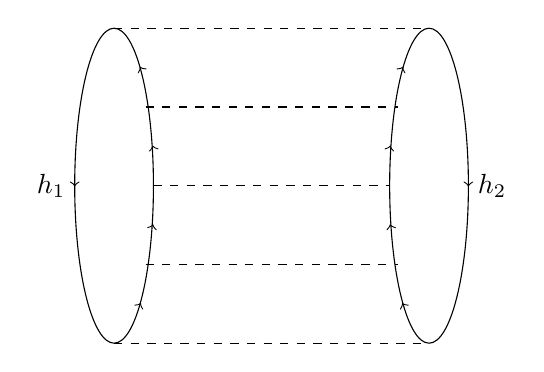
\begin{tikzpicture}
        \draw[-] (0,2) ellipse [x radius=0.5, y radius=2];
        \draw[-] (4,2) ellipse [x radius=0.5, y radius=2];
        \draw[dashed] (0,0)--(4,0);
        \draw[dashed] (0.4,1)--(3.6,1);
        \draw[dashed] (0.5,2)--(3.5,2);
        \draw[dashed] (0.4,3)--(3.6,3);
        \draw[dashed] (0,4)--(4,4);
        \draw[->] (-0.5,2.01)--(-0.5,1.99);
        \draw[->] (4.5,2.01)--(4.5,1.99);
        \draw[->] (0.33,0.49)--(0.34,0.51);
        \draw[->] (0.34,3.49)--(0.33,3.51);
        \draw[->] (3.67,0.49)--(3.66,0.51);
        \draw[->] (3.66,3.49)--(3.67,3.51);
        \draw[->] (0.49,1.49)--(0.495,1.51);
        \draw[->] (0.495,2.49)--(0.49,2.51);
        \draw[->] (3.51,1.49)--(3.505,1.51);
        \draw[->] (3.505,2.49)--(3.51,2.51);
        \node at (-0.8,2) {$h_1$};
        \node at (4.8,2) {$h_2$};
    \end{tikzpicture}
    \caption{\label{fig:csmbpt-5th}闭壳 MBPT 的五阶图,所有中间态都是 $2p2h$。}
\end{figure}

\section{$\hat{Q}$-box}
MBPT 得到有效相互作用与之前讨论的 MBPT 不同,没有参考态的说法。有效相互作用公式推导的核心是相似变换后的哈密顿量 $\mathcal{H}$ 如果满足 $Q\mathcal{H}P=0$,就能保证 $P\mathcal{H}P$ 的本征值与最初的 $H$ 相同。从 $Q\mathcal{H}P=0$ 出发,以 Lee-Suzuki 相似变换进行化简,也会出现 $QHQ$ 这样的项。从数学角度来看,相似变换后使 $Q\mathcal{H}P=0$,只对 $QHP$ 进行操作是不可能完成的,一定要同时操作 $QHQ$。从物理角度来看,退耦合 $P$ 与 $Q$ 空间的态,会不可避免地涉及到 $Q$ 空间内部的耦合,这也是之前提及的组态间的关联嵌套的体现。

除了微扰导致关联考虑不全的问题之外,$\hat{Q}$-box 有效相互作用还有一个问题,就是之前提到的 valence cluster expansion(VCE)。因为 MBPT 实际操作的都是组态相互作用的矩阵,但对于核芯上填 $A_v$ 个粒子的体系,应该存在一条,两条乃至 $A_v$ 条外腿的图。这些图全部纳入计算的难度太大了,因此 VCE 的思想是计算核芯上填充一个与两个核子的情况,此时只用计算一条与两条外腿的图。对一价核子与二价核子体系退耦合,得到适用于这些核的有效相互作用后,认为这个有效相互作用适用于整个壳,这就是 $\hat{Q}$-box 这种多体方法的截断。

随着核子数的增多,这么做从直觉上来看就不合适。少价核子体系的有效相互作用与更多核子体系的不应该相同,看上去很显然,但还不够有说服力。回顾具体求解过程,先对一核子体系求解 $\hat{S}$-box,得到有效相互作用的单体部分,再对二价核子体系求解 $\hat{Q}$-box,此时得到的 $P\mathcal{H}P$ 是二价核子体系的组态空间哈密顿量,并不是 Fock 空间的有效相互作用,需要从中减去单体部分才能得到有效相互作用的两体部分。如果继续考虑三价核子体系,需要减去单体与两体部分得到有效相互作用的三体部分。可以发现 $A_v$ 价核子体系的单体、两体直至 $A_v-1$ 体就是通过更少价核子体系获得的,求解 $A_v$ 价核子体系只是为了更新 $A_v$ 体部分。也就是说,在 $\hat{Q}$-box 的理论框架下,壳中其他原子核的单体和两体部分就等于只包含到两体图的有效相互作用。问题在于更多体部分直接缺失掉了。如果想包含这部分的影响,最直接的方式当然是使用能直接考虑三体部分的壳模型,退而求其次的方法是将这部分等效考虑进一体与二体,比如算二阶三体图 \cite{2019ma,2020coraggio-2vbetabeta,2020coraggio-ca,2022coraggio}。

VCE 导致关联缺失,所以结果算不准是显然的。也可以回归到有效相互作用理论的出发点看看 VCE 带来了什么。VCE 会导致退耦不干净,进而使模型空间的组态相互作用对角化与 FCI 产生偏差。这是因为对于大于两价核子的原子核,使用包含到两体图的有效相互作用,等价于这个相似变换没有清空 $Q\mathcal{H}P$,因为能清空 $Q\mathcal{H}P$ 的相似变换必然使 $P\mathcal{H}P$ 出现三体项,如果没有,耦合就没有完全退去。此外,阶数的截断也会导致 $Q\mathcal{H}P$ 不能完全清空。

\section{VS-IMSRG}
\subsection{退耦方式}
相比 MBPT,VS-IMSRG 直接操作 Fock 空间的哈密顿量。Fock 空间是所有粒子数的 Hilbert 空间的张量积。VS-IMSRG 的核心思想是,通过连续的相似变换将 Fock 空间的哈密顿量非对角元压低至 0,非对角元可以任意选取,这正是 IMSRG 直接推广到 VS-IMSRG 的方便之处。VS-IMSRG 选取的非对角元正是指标中涉及到模型空间外的态的矩阵元。这样做的好处是,用相似变换后的 Fock 空间哈密顿量 $H(s\to\infty)$ 写出组态空间哈密顿量 $\mathcal{H}$ 时,$Q\mathcal{H}P$ 块为 0,因为 $H(s\to\infty)$ 的矩阵元中涉及 $P$ 与 $Q$ 轨道耦合的项全都被演化为 0 了,自然就能保证 $P\mathcal{H}P$ 对角化与 FCI 得到一样的结果。

非对角元的选取不能太任意,出于计算考虑,非对角元选取过于广泛的话会导致对易中诱导出大量的三体算符,IMSRG(2) 截断失效 \cite{2017hergert}。这里先讨论退耦是怎么实现的。$Q\mathcal{H}P$ 的矩阵元可以用图 \ref{fig:imsrg-QHP} 的两体组态空间的矩阵元代表,更多粒子的组态空间相当于在此基础上添加旁观粒子,而单粒子组态空间则是去掉一个旁观粒子,都不影响这五种矩阵元的表达式。只需要将组成这五个组态空间的矩阵元的 Fock 空间非对角元演化为 0,就能保证 $Q\mathcal{H}P=0$。这里直接给出结果:

\begin{equation}
    H^{\mathrm{od}}=\{f_{ph},f_{pp^{\prime}},f_{hh^{\prime}},\Gamma_{pp^{\prime}hh^{\prime}},\Gamma_{pp^{\prime}vh},\Gamma_{pqvv^{\prime}}\}+\mathrm{H.c.}.\label{eqs:imsrg-Hod1}
\end{equation}

\begin{figure}[htbp]
  \centering
  \includegraphics[width=0.9\textwidth]{figure/imsrg-QHP.png}
  \caption{VS-IMSRG 退耦合的 $Q\mathcal{H}P$ 矩阵元,图取自 \cite{2017hergert}。}
  \label{fig:imsrg-QHP}
\end{figure}

注意这些需要压低的非对角元全是 normal order 后的矩阵元。
接下来用没有 normal order 的组态相互作用的公式推导这五类矩阵元,来得到需要压低的 Fock 空间非对角元。从下面的推导中可以看出,用没有 normal order 的哈密顿量进行推导,五种矩阵元有一系列的求和,形式比较复杂,如果把所有出现在求和中的非对角元全部压低为 0 会很麻烦。不过这些求和都能用 normal order 的哈密顿量简单地表示,所以直接压低 normal order 的非对角元更加容易。这也是 IMSRG 选择在 normal order 的公式形式下工作的另一个原因,首要原因自然是为了包含三体力。

直接使用最简洁的组态相互作用公式 \ref{eqs:ci-0},\ref{eqs:ci-1} 与 \ref{eqs:ci-2}。
在接下来的推导中,考虑价核子与核芯的存在,将组态写为 $|D\rangle=\prod_{i=1}^{m}a_{v_i}^\dagger\prod_{j=1}^{n}a_{c_j}^\dagger|0\rangle$,有 $m$ 个价核子,核芯有 $n$ 个核子,并不局限于两价核子空间。

第一类矩阵元是一个价核子由价空间轨道 $v_a$ 到价空间之外的 $q_b$,其他价核子都旁观,也就是 
\begin{equation}
    |D_f\rangle = \prod_{i\ne a} a_{v_i}^\dagger a_{q_b}^\dagger\prod_{j=1}^{n}a_{c_j}^\dagger|0\rangle,
\end{equation}
因此 
\begin{equation}
    \langle D_f|H|D_i\rangle_\mathrm{I} = (-1)^{\mathrm{permute}(v_a,q_b)}\left(h_{q_bv_a}+\sum_{k=1}^nV_{q_bc_kv_ac_k}+\sum_{l\ne a}V_{q_bv_lv_av_l}\right),
\end{equation}
$c_k$ 是对 hole 的求和,因此 
\begin{equation}
    h_{q_bv_a}+\sum_{k=1}^nV_{q_bc_kv_ac_k}=f_{q_bv_a},
\end{equation}
对核芯进行 normal order 时,$n_k=\theta(\epsilon_\mathrm{F}-\epsilon_k)$,也就是占据数只能为 0 或 1,前两项之和就变成了 normal order 后的单体项,这一项形如 $f_{qv}$,但对应非对角元的 $f_{pp'}$。而第三项形如 $\Gamma_{vqv'v''}$,但非对角元的选取是 $\Gamma_{pqvv'}$,这么定义是为了同时使第二类矩阵元也为 0。因为第三项是两体相互作用,应该出现在第二类矩阵元的图中,这是因为第一类矩阵元是用差 1 个轨道的组态相互作用公式计算的,也会包含差 2 个轨道的退化情况。

第二类矩阵元是两个价核子的轨道都改变了,至少有一个从 $v_a$ 到了 $q_c$,而另一个只要改变就可以,不一定非要离开价空间,假设从 $v_b$ 到了 $p_d$,$p=v$ 或 $q$,即
\begin{equation}
    |D_f\rangle=\prod_{i\ne a,b}a_{v_i}^\dagger a_{q_c}^\dagger a_{p_d}^\dagger \prod_{j=1}^na_{c_j}^\dagger|0\rangle,
\end{equation}
因此 
\begin{equation}
    \langle D_f|H|D_i\rangle_\mathrm{II} = (-1)^{\mathrm{permute}(v_a,v_b)+\mathrm{permute}(q_c,p_d)}V_{q_cp_dv_av_b},
\end{equation}
这也对应 $\Gamma_{pqvv'}$。

第三类矩阵元是价核子全都旁观,核芯中的一个核子从 $c_a$ 到任意 $p_b$,即
\begin{equation}
    |D_f\rangle=\prod_{i=1}^ma_{v_i}^\dagger a_{p_b}^\dagger\prod_{j\ne a}a_{c_j}^\dagger|0\rangle,
\end{equation}
因此
\begin{equation}
    \langle D_f|H|D_i\rangle_\mathrm{III} = (-1)^{\mathrm{permute}(c_a,p_b)}\left(h_{p_bc_a}+\sum_{k\ne a}V_{p_bc_kc_ac_k}+\sum_{l=1}^mV_{p_bv_lc_av_l}\right),
\end{equation}
一二项之和就是 $f_{p_bc_a}$,因为 $V_{p_bc_ac_ac_a}=0$,$k\ne a$ 的限制并不会引入额外的项。这对应非对角元的 $f_{ph}$。而第三项形如 $\Gamma_{pv'hv}$,对应非对角元的 $\Gamma_{pp'vh}$。同样第三项也是第四类矩阵元差 1 个轨道的特殊情况。

第四类矩阵元是核芯中的一个核子从 $c_a$ 到 $p_c$,一个价核子从 $v_b$ 到 $p_d$,即 
\begin{equation}
    |D_f\rangle = \prod_{i\ne b}a_{v_i}^\dagger a_{p_c}^\dagger a_{p_d}^\dagger\prod_{j\ne a}a_{c_j}^\dagger|0\rangle,
\end{equation}
因此 
\begin{equation}
    \langle D_f|H|D_i\rangle_\mathrm{IV} = (-1)^{\mathrm{permute}(c_a,v_b)+\mathrm{permute}(p_c,p_d)}V_{p_cp_dc_av_b},
\end{equation}
对应 $\Gamma_{pp'vh}$。

第五类矩阵元是核芯中两个核子从 $c_a,c_b$ 到 $p_c,p_d$,价核子全部旁观,即
\begin{equation}
    |D_f\rangle=\prod_{i=1}^ma_{v_i}^\dagger a_{p_c}^\dagger a_{p_d}^\dagger \prod_{j\ne a,b}a_{c_j}^\dagger|0\rangle,
\end{equation}
因此
\begin{equation}
    \langle D_f|H|D_i\rangle_\mathrm{V} = (-1)^{\mathrm{permute}(c_a,c_b)+\mathrm{permute}(p_c,p_d)}V_{p_cp_dc_ac_b},
\end{equation}
对应非对角元的 $\Gamma_{pp'hh'}$。

需要注意的是,经过上述讨论得到的非对角元实际上是
\begin{equation}
    H^{\mathrm{od}}_1=\{f_{ph},f_{qv},\Gamma_{pp'hh'},\Gamma_{pp'(vh\;\text{or}\;hv)},\Gamma_{(pq\;\text{or}\;qp)vv'}\}+\mathrm{H.c.},
\end{equation}
比 \ref{eqs:imsrg-Hod1} 少。为了使单体部分对角化,还可以额外添加单体非对角元,
\begin{equation}
    H^{\mathrm{od}}_2=\{f_{pp'},f_{hh'},H^{\mathrm{od}}_1\},
\end{equation}
这就与 \ref{eqs:imsrg-Hod1} 相同了。两体矩阵元下标的顺序,比如 $vh$ 或 $hv$ 的区别实际上只是一个相位。

由于最终的有效相互作用是对核芯而言的,因此实际上 VS-IMSRG 进行了两次退耦合,第一次对于分数填充的目标原子核进行,然后将算符写回真空态,再对核芯 normal order,进行第二次退耦合。但这里有个小问题,这五类矩阵元在第一步退耦合中是什么含义呢?在分数填充的参考态上填充两个粒子应该怎么算矩阵元呢?这需要打一个问号。在目前的公式体系中,第一步退耦合是通过修改流方程的占据数为分数来直接实现的,但这五类矩阵元公式是相对闭壳核推导出来的,分数填充时可能不一样(当然也有可能一样),有可能第一步退耦合无法把 $Q\mathcal{H}P$ 清空。但这个问题不严重,因为第二步退耦合肯定是能清空的。可以认为第一步退耦合就是为了考虑剩余三体力的影响才做的。

VS-IMSRG 在 Fock 空间中将非对角元演化为 0,这保证了价空间内所有原子核对应的组态空间哈密顿量都满足解耦条件。不过 VS-IMSRG 的重点并不在解耦条件上,而是在于相似变换。需要注意,相似变换的对象是 Fock 空间的 $H(s)$,但之前提到的解耦条件是对于组态空间哈密顿量而言的。Fock 空间哈密顿量的相似变换是否对应组态空间的相似变换?这并不是一个平凡的问题,但用组态相互作用的公式推了一下感觉没什么问题。

\subsection{正规序}
VS-IMSRG 完全在 normal order 的公式形式中工作,而 $\hat{Q}$-box 虽然也进行了 normal order,把三体力影响考虑进零体、一体与两体,但接着又把算符写回了真空态,最终是在非 normal order 的公式下推导的。


\subsection{核芯能量}
壳模型求出的本征值一定是相对于核芯的能量而不是总能量,这是因为壳模型中的组态其实是没有核芯轨道的,只有价空间的轨道,但多体方法必须对核心能量做出特殊处理,否则输出的有效相互作用就不对。

$\hat{Q}$-box 核芯能量的分离之前已经讨论过了,VS-IMSRG 则是将最终得到的有效相互作用减去 normal order 哈密顿量的零体项。可以看出,$\hat{Q}$-box 是在每一步推导中(无论是能量分母还是 Goldstone 图)都减去了核芯能量,而 VS-IMSRG 是在最后统一减去核芯能量,这个核芯能量是退耦合后的。



% MBPT 与 VS-IMSRG 虽然分别是在组态空间与 Fock 空间的两种方法,也有不做与做 normal order 的区别,但 \underline{核芯能量的分离与 normal order 没有任何关系}。尽管 VS-IMSRG 输出的 normal order 后的有效相互作用看上去总感觉多了对核芯轨道的求和,但这两套理论各自都是自洽的,所以这个问题没必要深究。

\subsection{截断}
接下来讨论截断方案,MBPT 的阶数截断以及 VCE 会导致 $Q\mathcal{H}P$ 不能完全清空,而 VS-IMSRG 的设计必定能清空壳内任意原子核的 $Q\mathcal{H}P$。这样的话 VS-IMSRG 不就完美无缺了吗?当然不是,VS-IMSRG(2) 截断了算符对易过程中诱导出的大于两体的算符,这带来的影响是,流方程不再严格相等,也就是说相似变换不再严格成立,这是 VS-IMSRG(2) 算不准的原因。

从这个角度看,非要讨论 VS-IMSRG(2) 丢失了哪些关联实属没事找事,因为 VS-IMSRG 与组态空间中的方法根本就不是一个理论体系,可以认为这就是个纯数学的变换。不过可以通过对流方程积分,看看对应 MBPT 的哪些图。


\part{Gamow 壳模型}

\chapter{Berggren 基矢}
\label{chap:berggren}

\section{复对称矩阵}
\label{sec:complex-symmetric-mat}

在 Berggren 基矢下,Gamow 壳模型的哈密顿量是复对称矩阵。在具体讨论 Gamow 壳模型的求解之前,先讨论复对称矩阵的性质。复对称矩阵 \(\bm{A}\) 满足 \(\bm{A}=\bm{A}^T\),并非厄米矩阵,因此并不一定能对角化,本征值也不一定是实数而是复数。

对于厄米矩阵 \(bm{H}\),本征方程
\begin{equation}
    \bm{H}\bm{v}=\lambda\bm{v},
\end{equation}
\(\lambda\) 为实数。两侧取厄米共轭得到
\begin{equation}
    \bm{v}^\dagger\bm{H}=\lambda\bm{v}^\dagger,
\end{equation}
同时右乘 \(\bm{v}\),
\begin{equation}
    \bm{v}^\dagger\bm{H}\bm{v}=\lambda\bm{v}^\dagger\bm{v},
\end{equation}
可以看出应该将本征矢量 \(\bm{v}\) 的归一化关系取为 \(\bm{v}^\dagger\bm{v}=1\)。以上讨论并非来自于线性代数的推导,但得出的结论与熟知的公式都是自洽的。对于复对称矩阵 \(\bm{A}\),重复以上流程,只是把取厄米共轭改为转置,归一化关系应为 \(\bm{v}^T\bm{v}=1\)。

对于 Dirac 记号,右矢仍为 \(\ket{\alpha}\),但左矢应记为 \(\bra{\tilde{\alpha}}=(\bra{\alpha})^*\),因为 Dirac 的 bra 符号默认是厄米共轭的。因此 Berggren 基矢的正交归一关系为
\begin{equation}
    \braket{\tilde{\alpha}}{\beta}=\delta_{\alpha\beta}.
\end{equation}
可观测量算符 \(\hat{O}\) 的矩阵元为
\begin{equation}
    O_{\alpha\beta}=\mel{\tilde{\alpha}}{\hat{O}}{\beta}.
\end{equation}


\chapter{Gamow 壳模型对角化}
\label{chap:gamow-diag}
Gamow 壳模型使用的 Berggren 基矢包含三种类型的单粒子态:束缚态,共振态与非共振散射态。而实验上能观测到的原子核的多体态是束缚态与宽度窄的共振态,散射态只是为满足基矢的完备性而被考虑,对角化想得到的多体态并不包含散射态。因此,Gamow 壳模型哈密顿量的对角化必须通过特殊的设计直接获得束缚态与共振态。

在讨论 Gamow 壳模型哈密顿量的对角化之前,先介绍厄米矩阵对角化使用的 Lanczos 算法。一般的壳模型是实对称矩阵,可通过 Lanczos 算法得到极端本征值及本征矢量。Lanczos 算法适合大规模稀疏矩阵的对角化,是因为只需要进行矩阵与向量的乘法,而不需要存储整个矩阵。对于稀疏矩阵,可以设计算法使得矩阵与向量相乘非常高效。




\part{全组态相互作用量子蒙特卡洛}

\chapter{FCIQMC 的理论框架}
\label{chap:fciqmc-frame}
\section{理论推导}
量子蒙特卡洛大致可以分为两类,一类是变分蒙特卡洛(VMC),其基础是变分法,从试探波函数出发,通过对波函数的变分优化寻找体系的基态,计算能量期望值的过程需要计算高维积分,VMC 用蒙特卡洛模拟的方式计算高维积分。另一类是投影量子蒙特卡洛,包括扩散蒙特卡洛(DMC),格林函数蒙特卡洛(GFMC),辅助场蒙特卡洛等,投影的本质就是解薛定谔方程。

全组态相互作用量子蒙特卡洛(FCIQMC)也是投影量子蒙特卡洛方法,出发点是虚时薛定谔方程,虽然将虚时间 $\tau$ 定义为 $it$,然而虚时薛定谔方程的本质是原本薛定谔方程的 Wick 转动,在转动之后虚时间也是实数。虚时薛定谔方程为
\begin{equation}
    \frac{\partial}{\partial\tau}\psi(\tau) = -H\psi(\tau),
\end{equation}
通过 Wick 转动变为虚时演化的目的在于,将 $e^{-iHt}$ 因子导致的振荡变为形如 $e^{-\tau H}$ 的指数衰减。这样就能够通过指数衰减将演化初始波函数中的非基态成分去掉,只留下基态。虚时薛定谔方程的解是
\begin{equation}
    \psi(\tau)=e^{-\tau H}\psi(\tau=0),
\end{equation}
虽然这里写的是等于,但因为波函数总是可以添加相因子的,因此其实可以写为
\begin{equation}
    \psi(\tau)\propto e^{-\tau H}\psi(\tau=0),
\end{equation}
在后面也会额外添加相因子,不过目前还是先从等于的这个式子出发,这样才能更好地理解后面添加相因子的意义。考虑 $H$ 的本征方程
\begin{equation}
    H\Psi_n=E_n\Psi_n,
\end{equation}
将虚时为 0 时的任意初始波函数用这组基矢展开,
\begin{equation}
    \psi(\tau=0)=\sum_nc_n\Psi_n,
\end{equation}
因此
\begin{equation}
    \psi(\tau)=e^{-\tau H}\sum_nc_n\Psi_n=\sum_nc_ne^{-\tau E_n}\Psi_n,
\end{equation}
虚时演化到 $\tau\to\infty$,因为 $E_0<E_1<E_2<\ldots$,
\begin{equation}
    e^{-\tau E_n}/e^{-\tau E_0}=e^{-\tau(E_n-E_0)}\to0,\quad n>0,
\end{equation}
此时主导的一定是基态波函数的系数,也即
\begin{equation}
    \lim_{\tau\to\infty}\psi(\tau)=c_0e^{-\tau E_0}\Psi_0.
\end{equation}
这还不完全是想要的基态波函数 $\Psi_0$,$c_0$ 可以直接归一化,但需要注意 $c_0\ne0$,也就是选取的演化初始波函数必须包含基态的成分,与基态完全正交显然是演化不出基态的。另外多出的 $e^{-\tau E_0}$ 因子也可以在虚时演化算符的定义中将其去掉,也就是前面提到的,可以把虚时薛定谔方程的解添加相因子,写为
\begin{equation}
    \psi(\tau)=e^{-\tau(H-E_0)}\psi(\tau=0),
\end{equation}
这种写法等价于如下虚时薛定谔方程
\begin{equation}
    -\odv{}{\tau}\psi(\tau)=(H-E_0)\psi(\tau).
\end{equation}

接下来在组态空间中进行虚时演化。组态空间的基矢是 Slater 行列式 \(\ket{D_i}\),将 $\psi(\tau)$ 在组态空间展开为
\begin{equation}
    \psi(\tau)=\sum_iC_i(\tau)\ket{D_i},
\end{equation}
代入虚时薛定谔方程得到
\begin{equation}
    -\odv{}{\tau}C_i(\tau)=\sum_j(H_{ij}-S\delta_{ij})C_j(\tau), 
\end{equation}
由于并不能在计算之前就知道 \(E_0\) 是多少,因此在实际计算时需要把 \(E_0\) 换为一个自适应调节的位移参数 \(S\)。

由于展开系数 \(C_i\) 有正也有负,无法将其分布情况转换为概率分布,因此 FCIQMC 将 \(N_i\) 个 walker 放在组态 \(\ket{D_i}\) 上,这些 walker 是带有符号的,因此可以表示负的展开系数。要求 walker 数目 \(N_i\) 与 \(C_i\) 成正比,因此 \(N_i\) 满足的演化方程离散化为
\begin{equation}
    -\adv{N_i}{\tau}=\sum_j(H_{ij}-S\delta_{ij})N_j,\label{eqs:fciqmc-master1}
\end{equation}
问题的关键就变成了设计一套算法,使 \(N_i\) 按照 \ref{eqs:fciqmc-master1} 演化。可以将 \ref{eqs:fciqmc-master1} 拆分为非对角项与对角项两部分,即
\begin{equation}
    -\adv{N_i}{\tau}=(H_{ii}-S)N_i+\sum_{j\ne i}H_{ij}N_j.\label{eqs:fciqmc-master2}
\end{equation}

先看非对角部分。对于每个 \(\ket{D_i}\),都有一系列 \(\ket{D_j}\) 与其相连,在 FCI 计算中这样的行列式非常多,不可能全纳入计算。这里就是 FCIQMC 的随机性的体现:通过蒙特卡洛方法采样波函数,保留重要的组态,以大幅度降低波函数的维数。简单来说,对于组态 \(\ket{D_i}\) 上的每个 walker,将其以一定的概率激发到某个与之相连的组态 \(\ket{D_j}\) 上,即在 \(\ket{D_j}\) 上以一定的概率生成 walker。这种表述与 \ref{eqs:fciqmc-master2} 的 \(i,j\) 记号其实是反着的,但 \cite{2009booth} 等文献都是把公式写为 \ref{eqs:fciqmc-master2},在语言表述中也是反过来。FCIQMC walkers 随机游走的详细过程是,目前演化到虚时间 \(\tau\),全空间的 walkers 分布为 \(\bm{N}(\tau)\),对每个有占据的行列式 \(\ket{D_i}\) 上的 \(N_i\) 个 walkers 中的每一个,将其以一定的概率激发到与 \(\ket{D_i}\) 相连的 \(\ket{D_j}\) 上,这个过程写为
\begin{equation}
    \Delta N_{j\gets i}=p_\text{spawn}(j|i)=\frac{\Delta
    \tau|H_{ji}|}{p_\text{gen}(j|i)},
\end{equation}
在确定性的对角化方法中,\(\ket{D_i}\) 的波函数系数 \(C_i\) 对所有其他的 \(C_j\) 都有贡献,贡献的强度由 \(H_{ij}\) 衡量。而在随机算法中,用 walker 数目 \(N_i\) 随机采样波函数的系数,目标是在每次演化中投影出重要的组态,以控制内存。因此不能在一步演化中完整考虑与 \(\ket{D_i}\) 相连的每一个 \(\ket{D_j}\),而是对 \(N_i\) 个 walkers 中的每个进行随机激发,就能在多步演化之后,从统计意义上达到 FCI 的效果。从 \(\ket{D_i}\) 激发到 \(\ket{D_j}\) 的概率为 \(p_\text{gen}(j|i)\),一种最简单的计算方法就是按照轨道占据等概率激发,当然还有更高效的激发算法,这会在后续讨论。激发概率出现在分母上相当于条件概率,walker 先选择激发到哪个 \(\ket{D_j}\),再按照 \ref{eqs:fciqmc-master2} 的要求于 \(\ket{D_j}\) 上生成对应数量的 walker。以上过程称为 spawning,实际计算中需要对 \(\bm{N}(\tau)\) 的每个行列式上的每个 walker 都进行以上的 spawning。

再看对角部分。这意味着在 \(\tau\to\tau+\Delta\tau\) 的演化中,\(\ket{D_i}\) 上的 \(N_i\) 个 walker 以
\begin{equation}
    p_\text{death}(i)=\Delta\tau(H_{ii}-S)
\end{equation}
的概率死亡。如果 \(p_\text{death}(i)<0\),则是以 \(-p_\text{death}(i)\) 的概率复制。由于以上演化全是在 \(\ket{D_i}\) 上进行的,只涉及 \(\ket{D_i}\) 上的 walkers,因此 \(N_i\) 死亡或克隆的数量就是
\begin{equation}
    \Delta N_i=-(H_{ii}-S)N_i\Delta\tau.
\end{equation}
这个过程称为 diagonal death/cloning。

这两个过程完成之后,得到了 \(\tau+\Delta\tau\) 时刻的一组新 walkers 分布。由于 walkers 都是自带符号的,接下来进行 annihilation 过程把符号相反的 walker 湮灭掉。该步骤是为了控制 walkers 的总数,也是 FCIQMC 方法处理费米子符号问题的关键步骤。

\section{计算步骤}
\subsection{预热}
FCIQMC 计算本质是对某个波函数虚时投影,提取出基态成分。也就是说需要将一定数量的 walkers 放在 \(\psi(\tau=0)\) 上作为计算的起点。


\section{费米子符号问题}
QMC 的本质是用概率分布模拟波函数。但量子力学玻恩的概率波诠释是波函数振幅(概率幅)的模方表示概率。然而 QMC 直接处理的是波函数的概率幅本身,对于费米子,由于需满足交换反对称性,波函数的概率幅一定是有正有负的(甚至还可能是复数),这就会导致 QMC 计算可观测量的平均值时,
\begin{equation}
    \expval{O}=\frac{\sum_i w_iO_i}{\sum_i w_i},
\end{equation}
权重 \(w_i\) 只采样了一部分概率幅,所以可能使分母的正负相抵,统计时平均值出现剧烈振荡,或者说统计噪声。另外,费米子符号问题还有另一种表现形式,投影量子蒙特卡洛方法求解的是薛定谔方程,但如果像 DMC 那样不在反对称化的空间中进行求解,可能无法保证费米子波函数的符号结构,导致投影出哈密顿量的无节点的最低能量解,该最低能量波函数不满足费米子的反对称性,这称为“Boson catastrophe”,也是费米子符号问题的一种体现。

通常解决费米子符号问题的方式是固定节点近似或约束路径方法,这些方法都需要比较好的试探波函数(或称为指导波函数)对波函数的节点结构进行限制,也是系统误差的主要来源。

而 FCIQMC 在反对称化的子空间,也就是组态空间进行,能够避免计算出玻色子基态。但仅仅如此并不能完全避免符号问题,因为即使在组态空间计算也有负的概率幅。在此基础上,符号相反的 walker 湮灭有助于提高体系的信噪比 \cite{2009booth},进一步压制符号问题;湮灭操作并非 FCIQMC 的首创,但相比在连续空间的 GFMC 与 DMC walker 的湮灭,离散的组态进行湮灭非常简单与自然。

然而费米子符号问题也没有被 FCIQMC 完全解决。最原始的 FCIQMC 算法存在的问题是,需要 walker 数目达到一定值才能稳定地收敛到基态。虚时演化收敛需要的最小 walker 数目与 Hilbert 空间的维数成比例,这会导致 FCIQMC 需要的计算量并不比 FCI 小多少。FCIQMC 虚时演化收敛需要的 walker 数目很大,这是费米子符号问题在 FCIQMC 这个方法中的表现形式。FCIQMC 演化收敛需要相当数量的 walkers,这是因为 \(\ket{\Psi_0}\) 与 \(-\ket{\Psi_0}\) 都是体系允许的基态波函数,然而在随机游走的过程中,可能会激发出属于 \(-\ket{\Psi_0}\) 的 walkers,导致大部分 walkers 是 \(\ket{\Psi_0}\) 的,而小部分 walkers 是 \(-\ket{\Psi_0}\) 的。这两部分 walkers 对基态波函数贡献的符号相反,且这种差别会通过指数的投影算符继续向后传播,导致随机产生的少数属于 \(-\ket{\Psi_0}\) 的 walkers 的效应被迅速放大,演化难以收敛。

\section{起始子近似}
体系波函数只有小部分的主导组态的概率幅绝对值比较大,绝大部分组态都是少占据或不占据的。在随机游走中,如果某个 walker spawn 到不被占据的行列式上,这个新 walker 的符号就完全由原来的 walker 决定,这就会出现符号波动,且会被指数投影迅速向之后的演化传播。也就是说,为了压制符号问题,限制可能符号不对的行列式上的 walkers 向未占据的行列式上 spawning 是一个直接的思路,这就是 initiator-FCIQMC(\textit{i}-FCIQMC)。

将 walker 数目大于给定阈值 \(n_a\) 的行列式称为 initiator 行列式,这些行列式的 walker 数目多,因此可认为符号是正确的,这些是 initiator 的 walkers 可以向未占据的行列式激发。不是 initiator 的 walkers 则不能向未占据的行列式激发,这能防止某个符号错误的 walker 主导与其相连的行列式的符号,并将错误的符号继续传播下去;非 initiator 的 walker 可以激发到已经有占据的行列式上,这些行列式上已经存在的 walkers 能够把这个符号错误的 walker 湮灭掉,阻止统计噪声的出现。

公式

已经证明 \textit{i}-FCIQMC 在任意的 walker 数目下都能实现稳定的演化 \cite{2019ghanem-as},但这是以引入系统误差为代价的。显然 initiator 近似相当于对真实的哈密顿量施加了截断

\subsection{Adaptive shift FCIQMC}
需要注意的是,adaptive shift 方法并不是必须要进行的,如果计算能力足够将所研究的体系用 \textit{i}-FCIQMC 算到对 walker 数收敛,系统误差就会被消除。也就是说 initiator 近似引入的系统误差并不是方法本身的缺陷。Adaptive shift 方法是计算能力不足以算收敛时引入的一种改进方法,其本质是用微扰将丢掉的部分补回来。

\chapter{FCIQMC 的计算实践}
\label{chap:fciqmc-practice}
作为一种新引入核物理的方法,FCIQMC 有大量的计算细节还不明确怎么处理是最好的,需要在测试中探索最合适的计算范式。本章结合计算结果,讨论的问题包括:对简单模型的基准测试,计算的参数如何设置,计算的收敛性如何,结果应该如何统计分析等。

\section{基准测试}
FCI 计算能精确对角化的小空间体系自然可以作为 FCIQMC 的基准测试。除此之外,量子化学对 FCIQMC 的测试,研究 FCIQMC 的行为与特征很多不是对真实的电子体系进行计算,而是使用 Hubbard 模型,Heisenberg 模型等。这些模型虽然不是都有严格解,但其物理图像简单,有物理意义明确的可调参数,并且用其他高精度方法计算也很简单。接下来对这些模型的哈密顿量进行简要介绍。
\subsection{Richardson pairing 模型}


\subsection{Hubbard 模型}

\section{计算设置}
原则上第一性原理计算是不需要引入额外参数的,但实际计算中一些需要手动调整的量或设置也是必不可少的,比如核力的 \(\hbar\omega\) 与 \(e_\text{max}\),模型空间,以及 FCIQMC 计算中会设置的虚时间步长 \(\dd\tau\),演化步数,walker 数目 \(N_w\),以及单激发、双激发概率,非整数 walker 数目截断阈值等很多细节的设置。虽然 \textit{ab initio} 计算不愿意称之为参数,但貌似也没有更合适的代替名词。不过这里还是将其广泛地称为“计算设置”,因为至少选模型空间轨道的这种设置不太能用某个“数”概括。
\subsection{虚时演化步长 \(\dd\tau\)}

\subsection{虚时演化步数}
投影量子蒙特卡洛方法对体系进行随机的虚时演化,并不能得到能量或波函数的确定值,只能在不同的虚时间下进行采样得到一批数据,需要对这些数据进行统计处理。以能量的计算为例,任何演化都不会在一开始就达到平衡或稳定,在稳定演化之前的波函数还混杂了大量非基态的成分。进行一定时间的虚时演化之后,波函数会调整为正确的基态波函数,能量也会在真实的基态能量附近上下波动,对这些稳定演化的数据进行采样与统计平均,才是正确的。

在 FCIQMC 中,演化步数需要在计算前进行设置。步数的设置既需要保证演化能够稳定,也需要在稳定后保证有足够的数据进行统计分析,同时为了节约计算时间,也不宜过多。图 \ref{fig:o16-evol-140k} 演化了 14 万步发现,增大演化步数并不会显著改善结果的统计误差,只要演化稳定了,能量的波动就在一个确定的范围内,并没有出现演化步数越多标准差越小的现象,要想提高统计精度,更应该增大 walker 数目 \(N_w\)。

\begin{figure}[!htbp]
  \centering
  \includegraphics[width=0.5\textwidth]{figure/fciqmc/O16_evol_140k.png}
  \caption{\ce{^16O} 虚时演化了 14 万步的过程。}
  \label{fig:o16-evol-140k}
\end{figure}

那演化步数应该取多少呢?在能接受的计算时间内自然是步数越多越安全,不过这也不是个过于重要的问题,因为 \(E(\tau)\) 的波动本身就不大,用几千个数据点统计分析已经足够了。这段讨论只是为了说明,更多的演化步数并不会改善结果的统计误差,只要不会少到影响统计分析即可。演化步数对统计分析的影响将会在后文进一步讨论。


\section{收敛性}
\subsection{虚时演化的稳定性}
如前所述,虚时演化的步数设置必须保证演化稳定。因此如何判断什么时刻进入稳定演化,以及哪些数据是可用的就成为了重要问题。最简单的做法就是画出 \(E\) 随着 \(\tau\) 的演化图,观察进入稳定演化的位置。但在 FCIQMC 中,使用热浴采样(heat-bath sampling)后能量会在演化的一开始就很稳定,很难看出在什么时刻演化变得稳定。不过在 FCIQMC 中还存在一个自适应调整的位移 \(S\) 用于控制 walker 数目 \(N_w\),在演化稳定之后 \(S\) 也会调整到基态能量附近,这样才能使 \(N_w\) 与 \(E\) 均稳定。由于 \(S(\tau)\) 的波动是比 \(E(\tau)\) 大的,因此 \(S(\tau)\) 也许是一个更好的判断演化何时稳定的标志。

用 N\(^2\)LO\(_{\text{opt}}\) 核力,\(e_\text{max}=8\),\(\hbar\omega=16\) MeV,以 adaptive-shift 方法,取 \(n_a=3,\Delta=0.5E_0\) 计算了 \ce{^16O},改变 \(N_w\) 数目,虚时演化如图 \ref{fig:o16-evol-nw} 所示。可以看出,\(S(\tau)\) 的波动确实比 \(E(\tau)\) 大,而且随着 \(N_w\) 的增加,两个量的波动都变小。这也是很好解释的,walker 数目越多,对基态能量有贡献的重要组态就能被更充分地包含进基态波函数中,\(S\) 与 \(E\) 自然会更加稳定。图 \ref{fig:o16-evol-nw} 未画 \(N_w<10^6\) 的结果,因为 walker 数目过少时 \(S(\tau)\) 的波动非常大。 
\begin{figure}[!htbp]
  \centering
  \includegraphics[width=1.0\textwidth]{figure/fciqmc/O16_evol_Nw.png}
  \caption{不同 \(N_w\) 下 \ce{^16O} 的虚时演化 20000 步的过程。}
  \label{fig:o16-evol-nw}
\end{figure}

\(E(\tau)\) 的演化比较稳定,没有很明显的波动,只是在演化初期有明显地下降,下降到一平台后就会围绕该平台稳定地波动。而 \(S(\tau)\) 则会先下降到低于基态能量,再调整到基态能量附近,围绕基态能量波动。相比 \(E(\tau)\),\(S(\tau)\) 稳定的位置更容易看出来,可以作为判断虚时演化稳定的指标。

从以上的计算中还可以看出 \(N_w\) 越大,\(S(\tau)\) 稳定所需要的步数越多。图 \ref{fig:o16-evol-nw} 中 \(N_w=10^6\) 经过 1500 步演化 \(S(\tau)\) 即稳定了,而 \(N_w=5\times10^6\) 则需要大约 3000 步才能稳定,增大到 \(N_w=10^7\) 则需要大约 5000 步才能稳定。

不过在实际计算中,使用更大的 \(N_w\) 得到的结果才能更好地降低系统误差,此时要想得到稳定的演化就需要更多的步数,比如 \(N_w=10^8\) 时演化 4000 步,\(S\) 还是显著低于 \(E\) 的,并未达到平台。但 \(N_w\) 越大,每一步的计算时间也越长。对此提出两种可能的解决方案。一种比较简单的做法是考虑到 \(N_w\) 较大时 \(E(\tau)\) 的波动本身就比较小,比如图 \ref{fig:o16-evol-nw} 中 \(N_w=10^7\) 时演化到 1500 步时就看不到 \(E(\tau)\) 在演化初期的下降了。这种做法比较简单,但让人担忧的是还是确定不了 \(E(\tau)\) 到底有没有真的稳定。因此另一种方案的设想是先用较小的 \(N_w\) 进行预演化,待 \(S(\tau)\) 稳定后以该波函数为初始波函数,用较大的 \(N_w\) 再次演化,这么做有可能用更少的步数就使得大 \(N_w\) 下的 \(S(\tau)\) 进入稳定阶段。

\section{块分析}




\appendix
\chapter{角动量耦合的公式}
\section{CG 系数}
\subsection{幺正性}
\begin{align}
  \sum_{J(M)}C_{j_1m_1j_2m_2}^{JM}C_{j_1m_1'j_2m_2'}^{JM}&=\delta_{m_1m_1'}\delta_{m_2m_2'}\label{app:cg-unitary-sumJM}\\
  \sum_{m_1m_2}C_{j_1m_1j_2m_2}^{JM}C_{j_1m_1j_2m_2}^{J'M'}&=\delta_{JJ'}\delta_{MM'}\label{app:cg-unitary-summ1m2}
\end{align}
注意在幺正性中,参与耦合的两个角动量 $j_1,j_2$ 是固定的,不存在对它们的求和。\ref{app:cg-unitary-sumJM} 的 $M$ 求和加括号是因为 $m_1,m_2$ 固定,$M$ 其实也固定了。一个方便的记忆方法是求和的量是一样的,求和上面等式右边 $\delta$ 的指标就是下面的量,反之亦然。

\subsection{对称性(“换底公式”)}
\begin{align}
  C_{j_1m_1j_2m_2}^{j_3m_3}&=(-1)^{j_1+j_2-j_3}C_{j_1-m_1j_2-m_2}^{j_3-m_3}=(-1)^{j_1+j_2-j_3}C_{j_2m_2j_1m_1}^{j_3m_3}\label{app:cg-changej1j2}\\
  &=(-1)^{j_1-m_1}\hat{j}_3\hat{j}_2^{-1}C_{j_3m_3j_1-m_1}^{j_2m_2}=(-1)^{j_2+m_2}\hat{j}_3\hat{j}_1^{-1}C_{j_2-m_2j_3m_3}^{j_1m_1}\\
  &=(-1)^{j_1-m_1}\hat{j}_3\hat{j}_2^{-1}C_{j_1m_1j_3-m_3}^{j_2-m_2}=(-1)^{j_2+m_2}\hat{j}_3\hat{j}_1^{-1}C_{j_3-m_3j_2m_2}^{j_1-m_1}\label{app:cg-changej1j2j3}
\end{align}
\ref{app:cg-changej1j2j3} 可以把在 CG 系数上下的角动量位置交换,因此我将其类比为“换底公式”。

\section{Wigner-3$j$ 符号}
$3j$ 符号顾名思义有三个角动量,分别是耦合前的两个与耦合后的一个,因此 $3j$ 符号与 CG 系数表达的物理一致,就是两个角动量的耦合。
\subsection{基本性质}
按顺序轮换列不变 \cite{book-zeng1}
\begin{equation}
  \begin{pmatrix}
    j_1&j_2&j_3\\m_1&m_2&m_3
  \end{pmatrix}=
  \begin{pmatrix}
    j_2&j_3&j_1\\m_2&m_3&m_1
  \end{pmatrix}=
  \begin{pmatrix}
    j_3&j_1&j_2\\m_3&m_1&m_2
  \end{pmatrix}\label{app:3j-loop}
\end{equation}

交换两列
\begin{equation}
  \begin{pmatrix}
    j_1&j_2&j_3\\m_1&m_2&m_3
  \end{pmatrix}
  =(-1)^{j_1+j_2+j_3}
  \begin{pmatrix}
    j_2&j_1&j_3\\m_2&m_1&m_3
  \end{pmatrix}\label{app:3j-change-column}
\end{equation}

\subsection{$3j$ 符号与 CG 系数的关系}
$3j$ 符号转 CG 系数 \cite{book-zeng1}
\begin{equation}
  \begin{pmatrix}
    j_1&j_2&j_3\\m_1&m_2&m_3
  \end{pmatrix}
  =(-1)^{j_1-j_2-m_3}\hat{j}_3^{-1}C_{j_1m_1j_2m_2}^{j_3-m_3}\label{app:3j-to-cg}
\end{equation}

CG 系数转 $3j$ 符号 
\begin{equation}
  C_{j_1m_1j_2m_2}^{j_3m_3}=(-1)^{j_1-j_2+m_3}\hat{j}_3  \begin{pmatrix}
    j_1&j_2&j_3\\m_1&m_2&-m_3
  \end{pmatrix}\label{app:cg-to-3j}
\end{equation}

\subsection{$3j$ 符号正交性}
\begin{align}
  \sum_{j_3m_3}\hat{j}_3^2
  \begin{pmatrix}
    j_1&j_2&j_3\\m_1&m_2&m_3
  \end{pmatrix}
  \begin{pmatrix}
    j_1&j_2&j_3\\m_1'&m_2'&m_3
  \end{pmatrix}
  &=\delta_{m_1m_1'}\delta_{m_2m_2'}\label{app:3j-ortho-sumjm}\\
  \sum_{m_1m_2}
  \begin{pmatrix}
    j_1&j_2&j_3\\m_1&m_2&m_3
  \end{pmatrix}
  \begin{pmatrix}
    j_1&j_2&j_3'\\m_1&m_2&m_3'
  \end{pmatrix}
  &=\hat{j}_3^{-2}\delta_{j_3j_3'}\delta_{m_3m_3'}\delta(j_1j_2j_3)\label{app:3j-ortho-summ1m2}
\end{align}
这里的 $\delta(j_1j_2j_3)$ 含义是判断 $j_1,j_2,j_3$ 能否满足角动量耦合的三角关系,满足时为 1,不满足时为 0。\ref{app:3j-ortho-summ1m2} 还有一种等价的写法是
\begin{equation}
  \sum_{m_1m_2m_3}
  \begin{pmatrix}
    j_1&j_2&j_3\\m_1&m_2&m_3
  \end{pmatrix}
  \begin{pmatrix}
    j_1&j_2&j_3'\\m_1&m_2&m_3'
  \end{pmatrix}
  =\delta_{j_3j_3'}\delta_{m_3m_3'}\delta(j_1j_2j_3)\label{app:3j-ortho-summ1m2m3}
\end{equation}
\ref{app:3j-ortho-summ1m2m3} 在 \ref{eqs:w-e-reverse-3j1} 推出 \ref{eqs:w-e-reverse-3j2} 中用到。虽然左侧的 $m_1+m_2+m_3=0$ 的限制存在,取定 $m_1$ 与 $m_2$ 后,$m_3$ 已经被取定,左侧对 $m_3$ 求和额外加上的所有东西都是 0,但右侧对 $m_3$ 求和就是乘上 $2j_3+1$,因此 \ref{app:3j-ortho-summ1m2m3} 成立。

\section{Wigner-6$j$ 符号}
$6j$ 符号则是有六个角动量,表达的物理是三个角动量的耦合,不过需注意 $j_1$ 与 $j_2$ 先耦合为 $j_{12}$ 再与 $j_3$ 耦合,这与 $j_2$ 先与 $j_3$ 耦合为 $j_{23}$ 再与 $j_1$ 耦合是不一样的。

\subsection{基本性质}
三列可以任意排序 \cite{book-zeng2}
\begin{equation}
  \begin{Bmatrix}
    j_1&j_2&j_3\\j_1'&j_2'&j_3'
  \end{Bmatrix}
  =\begin{Bmatrix}
    j_a&j_b&j_c\\j_a'&j_b'&j_c'
  \end{Bmatrix}
\end{equation}

上行中的任意两个数可以与下行的对应数对换
\begin{equation}
  \begin{Bmatrix}
    j_1&j_2&j_3\\j_1'&j_2'&j_3'
  \end{Bmatrix}
  =\begin{Bmatrix}
    j_1'&j_2'&j_3\\j_1&j_2&j_3'
  \end{Bmatrix}
\end{equation}

\subsection{CG 系数与 $6j$ 符号的关系}
\begin{align}
  &\sum C_{j_1m_1j_2m_2}^{j_{12}m_{12}}C_{j_{12}m_{12}j_3m_3}^{jm}C_{j_2m_2j_3m_3}^{j_{23}m_{23}}C_{j_1m_1j_{23}m_{23}}^{j'm'}\notag\\
  ={}&\delta_{jj'}\delta_{mm'}(-1)^{j_1+j_2+j_3+j}\hat{j}_{12}\hat{j}_{23}
  \begin{Bmatrix}
    j_1&j_2&j_{12}\\j_3&j&j_{23}
  \end{Bmatrix}\label{app:cg-to-6j}
\end{align}
求和是对 $m_1,m_2,m_3,m_{12},m_{23}$ 进行的,$m,m'$ 固定。这个公式在使用时一个方便的方法是,寻找两种角动量耦合的顺序,一个是 $j_1$ 与 $j_2$ 先耦合为 $j_{12}$,再与 $j_3$ 耦合为 $j$,另一个是 $j_2$ 与 $j_3$ 先耦合为 $j_{23}$,再与 $j_1$ 耦合为 $j'$,根据这个顺序替换公式里的记号就方便了。

\subsection{$6j$ 符号有一个数为 0}
\begin{equation}
  \begin{Bmatrix}
    j_1&j_2&j_3\\j_4&j_5&0
  \end{Bmatrix}
  =\frac{(-1)^{j_1+j_2+j_3}\delta_{j_1j_5}\delta_{j_2j_4}}{\sqrt{(2j_1+1)(2j_2+1)}}\label{app:6j-onej-0}
\end{equation}

\section{Wigner $9j$ 符号}
$9j$ 符号表达的是四个角动量的耦合,另外在 \cite{jin-goldstone} 中会用到归一化的 $9j$ 符号,定义为
\begin{equation}
  \begin{bmatrix}
    j_1&j_2&j_{12}\\
    j_3&j_4&j_{34}\\
    j_{13}&j_{24}&J
  \end{bmatrix}=\hat{j}_{12}\hat{j}_{13}\hat{j}_{23}\hat{j}_{24}
  \begin{Bmatrix}
    j_1&j_2&j_{12}\\
    j_3&j_4&j_{34}\\
    j_{13}&j_{24}&J
  \end{Bmatrix}.
\end{equation}

\subsection{$9j$ 符号有一个数为 0}
\begin{equation}
  \begin{Bmatrix}
    j_1&j_2&j_{12}\\
    j_3&j_4&j_{34}\\
    j_{13}&j_{24}&J
  \end{Bmatrix}=\frac{(-1)^{j_2+j_3+j_{12}+j_{13}}\delta_{j_{12}j_{34}}\delta_{j_{13}j_{24}}}{\sqrt{(2j_{12}+1)(2j_{13}+1)}}
  \begin{Bmatrix}
    j_1&j_2&j_{12}\\
    j_4&j_3&j_{13}
  \end{Bmatrix}.
\end{equation}

\chapter{跃迁密度矩阵}
由于在正文中 OBTD 与 TBTD 的推导并没有用 \cite{brown} 引入张量积算符的做法,为了保持正文的简洁,将 \cite{brown} 的做法放在此处。

\section{OBTD}
使用 Wigner-Eckart 定理 \ref{eqs:w-e-3j},将算符矩阵元约化
\begin{equation}
  \langle \alpha|\hat{O}^\lambda_\mu|\beta\rangle =  (-1)^{j_\alpha - m_\alpha} \mqty(j_\alpha&\lambda&j_\beta\\-m_\alpha&\mu&m_\beta) \langle k_\alpha||\hat{O}^\lambda||k_\beta\rangle,
\end{equation}
下面处理产生湮灭算符,这是两个算符的乘积,需要使用球张量算符的张量积公式 \cite{2007suhonen},用秩为 \(L_1\) 与 \(L_2\) 的球张量算符 \(\hat{T}^{L_1}\) 与 \(\hat{T}^{L_2}\) 构造秩为 \(L\) 的球张量算符,
\begin{equation}
  \hat{T}^L_M=\sum_{M_1M_2}C_{L_1M_1L_2M_2}^{LM}\hat{T}^{L_1}_{M_1}\hat{T}^{L_2}_{M_2}\equiv[\hat{T}^{L_1}\otimes \hat{T}^{L_2}]^L_M,\label{eqs:tensor-op-prod}
\end{equation}
另外,秩为 \(L\) 的张量算符 \(\hat{T}^L_M\),其厄米共轭 \((\hat{T}^L_M)^\dag\) 并不是秩为 \(L\) 的张量算符。存在关系 \cite{2007suhonen}
\begin{equation}
  (\hat{T}^L_M)^\dag = (-1)^{M}\hat{T}^L_{-M},
\end{equation}
因此 
\begin{equation}
  \tilde{\hat{T}}^L_M \equiv (-1)^{p+M}(\hat{T}^L_{-M})^\dag\label{eqs:tilde-tensor-op}
\end{equation}
是球张量算符。根据 \cite{brown} 的说法,\(p\) 可任意选择,当秩 \(L\) 为整数时可以取 \(p=0\),为半整数时可以取 \(p=L\),以保证相位为实数。对于产生湮灭算符,\(a^\dag=a^\dag_{km}\) 是秩为 \(j\) 的球张量算符,为半整数,因此湮灭算符变为球张量算符的变换取为
\begin{equation}
  \tilde{a}_{km} =(-1)^{j+m}(a^\dag_{k,-m})^\dag=(-1)^{j+m} a_{k,-m},
\end{equation}
由此可得
\begin{equation}
  a_{km}=(-1)^{j-m}\tilde{a}_{k,-m}.
\end{equation}

将湮灭算符换为球张量算符,另外为了与 \ref{eqs:tensor-op-prod} 的形式一致,用 \ref{app:3j-to-cg} 将 \(3j\) 系数符号换为 CG 系数,得到
\begin{align}
  \hat{O}^\lambda_\mu &=\sum_{\alpha\beta}(-1)^{j_\alpha - m_\alpha}(-1)^{j_\alpha+j_\beta+\lambda}\mqty(j_\alpha&j_\beta&\lambda\\-m_\alpha&m_\beta&\mu)\langle k_\alpha||\hat{O}^\lambda||k_\beta\rangle a^\dag_\alpha a_\beta\notag\\
  &=\sum_{k_\alpha k_\beta}\langle k_\alpha||\hat{O}^\lambda||k_\beta\rangle\sum_{m_\alpha m_\beta}(-1)^{j_\alpha-m_\alpha+\lambda-\mu+1}\hat{\lambda}^{-1}C_{j_\alpha -m_\alpha j_\beta m_\beta}^{\lambda -\mu}a^\dag_\alpha a_\beta\notag\\
  &=\sum_{k_\alpha k_\beta}\langle k_\alpha||\hat{O}^\lambda||k_\beta\rangle\sum_{m_\alpha m_\beta}(-1)^{j_\beta + m_\beta+1}\hat{\lambda}^{-1}C_{j_\alpha m_\alpha j_\beta -m_\beta}^{\lambda\mu}a^\dag_{k_\alpha m_\alpha} (-1)^{j_\beta - m_\beta}\tilde{a}_{k_\beta -m_\beta}\notag\\
  &=\sum_{k_\alpha k_\beta}\langle k_\alpha||\hat{O}^\lambda||k_\beta\rangle \hat{\lambda}^{-1}\sum_{m_\alpha m_\beta}C_{j_\alpha m_\alpha j_\beta -m_\beta}^{\lambda\mu} a^\dag_{k_\alpha m_\alpha}\tilde{a}_{k_\beta -m_\beta}\notag\\
  &=\sum_{k_\alpha k_\beta}\langle k_\alpha||\hat{O}^\lambda||k_\beta\rangle \hat{\lambda}^{-1}[a^\dag_{k_\alpha}\otimes \tilde{a}_{k_\beta}]^\lambda_\mu.\label{eqs:ob-op-to-tensor-prod}
\end{align}
由此计算初态 \(\ket{\Psi_i}\) 与末态 \(\ket{\Psi_f}\) 之间的约化跃迁矩阵元
\begin{equation}
  \langle \Psi_f||\hat{O}^\lambda||\Psi_i\rangle = \sum_{k_\alpha k_\beta}\langle k_\alpha||\hat{O}^\lambda||k_\beta\rangle \hat{\lambda}^{-1}\langle \Psi_f||[a^\dag_{k_\alpha}\otimes \tilde{a}_{k_\beta}]^\lambda||\Psi_i\rangle.
\end{equation}
定义 OBTD 为 
\begin{equation}
  \text{OBTD}(fik_\alpha k_\beta\lambda) \equiv \hat{\lambda}^{-1}\langle \Psi_f||[a^\dag_{k_\alpha}\otimes \tilde{a}_{k_\beta}]^\lambda||\Psi_i\rangle,
\end{equation}
因此约化跃迁矩阵元的计算就简化为了
\begin{equation}
  \langle \Psi_f||\hat{O}^\lambda||\Psi_i\rangle = \sum_{k_\alpha k_\beta}\langle k_\alpha||\hat{O}^\lambda||k_\beta\rangle\;\text{OBTD}(fik_\alpha k_\beta\lambda).
\end{equation}

不过多体计算得到的波函数通常是 \(m\)-scheme 的,因此还需要通过 \(m\)-scheme 的波函数计算出 OBTD。使用 \ref{eqs:wigner-eckart} 得到
\begin{equation}
  \langle \Psi_f||[a^\dag_{k_\alpha}\otimes \tilde{a}_{k_\beta}]^\lambda||\Psi_i\rangle = \frac{\langle \Psi_f|[a^\dag_{k_\alpha}\otimes \tilde{a}_{k_\beta}]^\lambda_\mu|\Psi_i\rangle}{(-1)^{J_f - M_f} \mqty(J_f&\lambda&J_i\\-M_f&\mu&M_i)},
\end{equation}
\cite{brown} 的这个公式应该是写错了,分母的 \(3j\) 符号第一列写的是 \(J_f\) 与 \(M_f\),不知道原因。而 KSHELL 代码中写的公式则是用 \ref{eqs:w-e-cg1} 与 \ref{app:cg-changej1j2j3} 将 OBTD 换为单线矩阵元,这样才能在 \(m\)-scheme 下计算,即 
\begin{equation}
  \text{OBTD}(fik_\alpha k_\beta\lambda)=\hat{\lambda}^{-1}\frac{\langle \Psi_f|[a^\dag_{k_\alpha}\otimes \tilde{a}_{k_\beta}]^\lambda_\mu|\Psi_i\rangle}{\hat{\lambda}^{-1}(-1)^{J_i-M_i}C_{J_iM_iJ_f-M_f}^{\lambda-\mu}}=\frac{(-1)^{J_i-M_i}}{C_{J_iM_iJ_f-M_f}^{\lambda-\mu}}\langle \Psi_f|[a^\dag_{k_\alpha}\otimes \tilde{a}_{k_\beta}]^\lambda_\mu|\Psi_i\rangle,
\end{equation}
接下来再把 OBTD 中的张量积用 \ref{eqs:tensor-op-prod} 展开,得到
\begin{equation}
  \langle \Psi_f|[a^\dag_{k_\alpha}\otimes \tilde{a}_{k_\beta}]^\lambda_\mu|\Psi_i\rangle = \sum_{m_\alpha m_\beta}(-1)^{j_\beta-m_\beta}C_{j_\alpha m_\alpha j_\beta -m_\beta}^{\lambda\mu} \langle \Psi_f|a^\dag_\alpha a_\beta|\Psi_i\rangle.
\end{equation}

\section{TBTD}
两体算符
\begin{equation}
  \hat{T}^\lambda_\mu=\frac{1}{4}\sum_{\alpha\beta\gamma\delta}\langle \alpha\beta|\hat{T}^\lambda_\mu|\gamma\delta\rangle a_\alpha^\dag a_\beta^\dag a_\delta a_\gamma,
\end{equation}
先将算符的矩阵元转到角动量耦合表象下,
\begin{align}
  \hat{T}^\lambda_\mu ={}& \frac14\sum_{k_\alpha k_\beta k_\gamma k_\delta}\sum_{m_\alpha m_\beta m_\gamma m_\delta}\mel{k_\alpha m_\alpha k_\beta m_\beta}{\hat{T}^\lambda_\mu}{k_\gamma m_\gamma k_\delta m_\delta}a^\dag_{k_\alpha m_\alpha} a^\dag_{k_\beta m_\beta} a_{k_\delta m_\delta} a_{k_\gamma m_\gamma}\notag\\
  ={}&\frac14\sum_{k_\alpha k_\beta k_\gamma k_\delta}\sum_{JMJ'M'}\frac1{N_{k_\alpha k_\beta}N_{k_\gamma k_\delta}}\mel{k_\alpha k_\beta JM}{\hat{T}^\lambda_\mu}{k_\gamma k_\delta J'M'}\notag\\
  &\times\sum_{m_\alpha m_\beta m_\gamma m_\delta}C_{j_\alpha m_\alpha j_\beta m_\beta}^{JM}C_{j_\gamma m_\gamma j_\delta m_\delta}^{J'M'}a^\dag_{k_\alpha m_\alpha} a^\dag_{k_\beta m_\beta} a_{k_\delta m_\delta} a_{k_\gamma m_\gamma},
\end{align}
单体算符的推导中先用 \ref{eqs:tensor-op-prod} 将产生湮灭算符的乘积耦合为张量积,再逆用 \ref{eqs:tensor-op-prod} 以在 \(m\)-scheme 下计算矩阵元。这么做是因为只有张量积算符才能用 Wigner-Eckart 定理,进而才能定义出 \(j\)-scheme 下的 OBTD。但是因为波函数是 \(m\)-scheme 的,所以还要再倒回去。但是对两个产生算符与两个湮灭算符,怎么定义球张量算符与张量积是一个问题。\cite{brown} 的做法是考虑耦合的两体态 \(\ket{k_\alpha k_\beta JM}\),将其视为一个产生算符 \(A^\dag\) 作用于真空态的产物,
\begin{equation}
  A^\dag(k_\alpha k_\beta JM)\ket{0}\equiv \ket{k_\alpha k_\beta JM},
\end{equation}
因此 
\begin{equation}
  A^\dag(k_\alpha k_\beta JM)=N_{k_\alpha k_\beta}\sum_{m_\alpha m_\beta}C_{j_\alpha m_\alpha j_\beta m_\beta}^{JM}a^\dag_{k_\beta m_\beta}a^\dag_{k_\alpha m_\alpha},
\end{equation}
这其实就可以直接使用 \ref{eqs:tensor-op-prod} 得到
\begin{equation}
  A^\dag(k_\alpha k_\beta JM)=-N_{k_\alpha k_\beta}[a^\dag_{k_\alpha}\otimes a^\dag_{k_\beta}]^J_M.
\end{equation}
湮灭算符为
\begin{equation}
  A(k_\alpha k_\beta JM)=\{A^\dag(k_\alpha k_\beta JM)\}^\dag=N_{k_\alpha k_\beta}\sum_{m_\alpha m_\beta}C_{j_\alpha m_\alpha j_\beta m_\beta}^{JM}a_{k_\alpha m_\alpha} a_{k_\beta m_\beta},
\end{equation}
同样变为球张量算符
\begin{align}
  \tilde{A}(k_\alpha k_\beta JM) &= (-1)^{J+M}\{A^\dag(k_\alpha k_\beta J,-M)\}^\dag\notag\\
  &= N_{k_\alpha k_\beta}(-1)^{J+M}\sum_{m_\alpha m_\beta}C_{j_\alpha m_\alpha j_\beta m_\beta}^{J -M} a_{k_\alpha m_\alpha} a_{k_\beta m_\beta}\notag\\
  &= N_{k_\alpha k_\beta} (-1)^{J+M}\sum_{m_\alpha m_\beta}(-1)^{j_\alpha+j_\beta-J}C_{j_\alpha -m_\alpha j_\beta -m_\beta}^{J M}(-1)^{j_\alpha - m_\alpha} \tilde{a}_{k_\alpha -m_\alpha} (-1)^{j_\beta - m_\beta} \tilde{a}_{k_\beta -m_\beta}\notag\\
  &=N_{k_\alpha k_\beta}[\tilde{a}_{k_\alpha}\otimes \tilde{a}_{k_\beta}]^J_M,
\end{align}
推导中用了 \(-M=m_\alpha+m_\beta\),以及默认 \(J\) 为整数,将 \((-1)^M\) 换为了 \((-1)^{-M}\)。我并不确定这是不是来自于 \ref{eqs:tilde-tensor-op} 中的相位约定,虽然 \cite{brown,book-zeng2} 写的都是 \((-1)^{p+M}\),但 \cite{brown} 在这个公式的推导中又把 \(+M\) 偷偷换为了 \(-M\)。不过在两体态的情况肯定是可以的。关于这个符号约定 \cite{book-zeng2} 也并未提 \(p\) 任取的事情,而是直接取了算符的秩 \(L\);而 \cite{brown} 虽然说秩为整数时取 \(p=0\),但在这个推导反而取了 \(p=L\) 的形式。看上去只有这么取,一些不想要的负号才能消失。

定义好耦合表象两体态的产生湮灭算符之后,\(\hat{T}^\lambda_\mu\) 可以写为
\begin{align}
  \hat{T}^\lambda_\mu = \frac14\sum_{k_\alpha k_\beta k_\gamma k_\delta}\sum_{JMJ'M'}\frac1{N_{k_\alpha k_\beta}^2N_{k_\gamma k_\delta}^2}\mel{k_\alpha k_\beta JM}{\hat{T}^\lambda_\mu}{k_\gamma k_\delta J'M'}A^\dag(k_\alpha k_\beta JM)A(k_\gamma k_\delta J'M'),
\end{align}
为了与二次量子化的四个单粒子产生湮灭算符的顺序相对应,在换为两体态的产生湮灭算符时交换顺序各自产生一个负号,消去了。接下来就可以将湮灭算符换为球张量算符并使用 \ref{eqs:tensor-op-prod},因为此时两体态的产生湮灭算符形式上与单粒子没有任何区别,角动量从半整数变为整数也不会额外产生相位,因此这个推导完全重复 \ref{eqs:ob-op-to-tensor-prod} 的过程,直接写出
\begin{align}
  \hat{T}^\lambda_\mu ={}& \frac14\sum_{k_\alpha k_\beta k_\gamma k_\delta JJ'}\frac1{N_{k_\alpha k_\beta}^2{N_{k_\gamma k_\delta}^2}}\langle k_\alpha k_\beta J||\hat{T}^\lambda||k_\gamma k_\delta J'\rangle \hat{\lambda}^{-1}[A^\dag(k_\alpha k_\beta J)\otimes \tilde{A}(k_\gamma k_\delta J')]^\lambda_\mu\notag\\
  ={}& \sum_{k_\alpha\le k_\beta, k_\gamma\le k_\delta}\sum_{JJ'}\langle k_\alpha k_\beta J||\hat{T}^\lambda||k_\gamma k_\delta J'\rangle \hat{\lambda}^{-1}[A^\dag(k_\alpha k_\beta J)\otimes \tilde{A}(k_\gamma k_\delta J')]^\lambda_\mu.\label{eqs:tb-op-to-tensor-prod}
\end{align}

同样计算初态 \(\ket{\Psi_i}\) 与末态 \(\ket{\Psi_f}\) 之间的约化跃迁矩阵元
\begin{equation}
  \mel{\Psi_f}{\hat{T}^\lambda_\mu}{\Psi_i} = \sum_{k_\alpha\le k_\beta, k_\gamma\le k_\delta}\sum_{JJ'}\langle k_\alpha k_\beta J||\hat{T}^\lambda||k_\gamma k_\delta J'\rangle \hat{\lambda}^{-1}\langle \Psi_f||[A^\dag(k_\alpha k_\beta J)\otimes \tilde{A}(k_\gamma k_\delta J')]^\lambda||\Psi_i\rangle,
\end{equation}
并定义 TBTD 
\begin{equation}
  \text{TBTD}(fikJJ'\lambda)\equiv \hat{\lambda}^{-1}\langle \Psi_f||[A^\dag(k_\alpha k_\beta J)\otimes \tilde{A}(k_\gamma k_\delta J')]^\lambda||\Psi_i\rangle,
\end{equation}
将 TBTD 的 \(k_\alpha,k_\beta,k_\gamma,k_\delta\) 依赖简记为 \(k\),因此两体算符的约化跃迁矩阵元为
\begin{equation}
  \langle \Psi_f||\hat{T}^\lambda||\Psi_i\rangle = \sum_{k_\alpha\le k_\beta, k_\gamma\le k_\delta}\sum_{JJ'}\langle k_\alpha k_\beta J||\hat{T}^\lambda||k_\gamma k_\delta J'\rangle\;\text{TBTD}(fikJJ'\lambda).
\end{equation}

TBTD 换回单线矩阵元
\begin{equation}
  \text{TBTD}(fikJJ'\lambda)=\frac{(-1)^{J_i-M_i}}{C_{J_iM_iJ_f-M_f}^{\lambda-\mu}}\langle \Psi_f|[A^\dag(k_\alpha k_\beta J)\otimes \tilde{A}(k_\gamma k_\delta J')]^\lambda_\mu|\Psi_i\rangle,
\end{equation}
并在 \(m\)-scheme 下计算,
\begin{align}
  \langle \Psi_f|[A^\dag(k_\alpha k_\beta J)\otimes \tilde{A}(k_\gamma k_\delta J')]^\lambda_\mu|\Psi_i\rangle ={}&\sum_{MM'}(-1)^{J'-M'}C_{JM J'-M'}^{\lambda\mu}\notag\\
  &\times\langle \Psi_f|A^\dag(k_\alpha k_\beta JM)A(k_\gamma k_\delta J'M')|\Psi_i\rangle\notag\\
  ={}& N_{k_\alpha k_\beta} N_{k_\gamma k_\delta}\sum_{MM'}(-1)^{J'-M'}C_{JM J'-M'}^{\lambda\mu}\notag\\
  &\times\sum_{m_\alpha m_\beta m_\gamma m_\delta}C_{j_\alpha m_\alpha j_\beta m_\beta}^{JM}C_{j_\gamma m_\gamma j_\delta m_\delta}^{J'M'}\mel{\Psi_f}{a^\dag_\alpha a^\dag_\beta a_\delta a_\gamma}{\Psi_i}.
\end{align}

\bibliography{bib/many_body.bib}

\end{document}